% ---------------------------------------------------------------------------------
% Main tex file
% $Id: Thesis.tex,v 1.55 2012/07/23 16:36:02 matsch Exp $

\documentclass[
twoside=true,
headsepline,     % Line under page header
headings=normal,
open=right,
numbers=noenddot, % Otherwise there will be a dot after the chapter numbering in case letters are used somewhere e.g. in the appendix
a4paper,
11pt
]{scrreprt} %report scrreprt
\addtolength{\topmargin}{-0.2cm}
\setlength{\textwidth}{15cm}
\setlength{\textheight}{22.4cm}
\setlength{\oddsidemargin}{0cm}
\setlength{\evensidemargin}{0.85cm} 

\usepackage[automark,headsepline]{scrpage2}
\pagestyle{scrheadings}
\clearscrheadfoot
\ihead{\headmark}
\ohead{\pagemark}
\cfoot{}
\setcounter{secnumdepth}{3}
\setcounter{tocdepth}{3}



% Alter some LaTeX defaults for better treatment of figures,
% from http://mintaka.sdsu.edu/GF/bibliog/latex/floats.html
% See p.105 of "TeX Unbound" for suggested values.
% See pp. 199-200 of Lamport's "LaTeX" book for details.
% General parameters, for ALL pages:
\renewcommand{\topfraction}{0.9}	% max fraction of floats at top
\renewcommand{\bottomfraction}{0.8}	% max fraction of floats at bottom
% Parameters for TEXT pages (not float pages):
%\setcounter{topnumber}{2}
%\setcounter{bottomnumber}{2}
%\setcounter{totalnumber}{4}     % 2 may work better
%\setcounter{dbltopnumber}{2}    % for 2-column pages
\renewcommand{\dbltopfraction}{0.9}	% fit big float above 2-col. text
\renewcommand{\textfraction}{0.07}	% allow minimal text w. figs
% Parameters for FLOAT pages (not text pages):
\renewcommand{\floatpagefraction}{0.7}	% require fuller float pages
% N.B.: floatpagefraction MUST be less than topfraction !!
\renewcommand{\dblfloatpagefraction}{0.7}	% require fuller float pages
% remember to use [htp] or [htpb] for placement

\usepackage{scrhack}
\usepackage{afterpage}
\usepackage{caption}
\usepackage{subcaption}
\usepackage{amsfonts}
\usepackage{pifont}
\usepackage{amsmath}  % Correct size switching in mathmode when using \text{} instead of \textrm{}
\usepackage{amssymb} 
\usepackage{amstext} 
\usepackage{cite}
\usepackage{graphicx}
\usepackage{booktabs}
\usepackage{tabularx}
\usepackage{multirow}
\usepackage{setspace}
\usepackage{rotating}
\usepackage{float}
\usepackage{afterpage}
\usepackage{verbatim}
\usepackage{textcomp,gensymb}
\usepackage[bottom]{footmisc}
\usepackage{makecell}
\usepackage{pdflscape}
\usepackage{hvfloat}
\usepackage[makeroom]{cancel}
\usepackage{enumerate}
\usepackage[]{placeins}
\usepackage[]{units}
\usepackage[super]{nth}
\usepackage{fixmath}
\usepackage{lineno}
\usepackage{seqsplit}
\usepackage{amsmath,amssymb}
\usepackage{slashed}
\usepackage{bbm}

% \usepackage{subfigure}
% \usepackage{subfig}
%\usepackage{hepnames}
% \usepackage{ptdr-definitions}
%
%\usepackage{setspace}
%\doublespacing

\hyphenation{Super-sym-me-try}
\hyphenation{maximum-like-li-hood}
\hyphenation{brems-strahl-ung}
\hyphenation{PFMET-no-Mu}

% ---------------------------------------------------------------------------------
% Collection of user-defined commands
% $Id: definitions.tex,v 1.46 2012/07/23 16:36:01 matsch Exp $

\usepackage{amsmath}
\usepackage{xspace}

\newcommand{\figmultican}[1]{
  \centering
  \includegraphics[width=0.85\textwidth]{figures/#1}
}
\newcommand{\figone}[1]{
  \centering
  \includegraphics[width=0.49\textwidth]{figures/#1}
}
\newcommand{\figtwo}[2]{
  \centering
  \begin{tabular}{@{}c@{}p{0.02\textwidth}@{}c@{}}
    \includegraphics[width=0.49\textwidth]{figures/#1} & &
    \includegraphics[width=0.49\textwidth]{figures/#2} \\
  \end{tabular}
}
\newcommand{\figthree}[3]{
  \centering
  \begin{tabular}{@{}c@{}p{0.02\textwidth}@{}c@{}}
    \includegraphics[width=0.49\textwidth]{figures/#1} & &
    \includegraphics[width=0.49\textwidth]{figures/#2} \\
    \includegraphics[width=0.49\textwidth]{figures/#3} & & \\
  \end{tabular}
}
\newcommand{\figfour}[4]{
  \centering
  \begin{tabular}{@{}c@{}p{0.02\textwidth}@{}c@{}}
    \includegraphics[width=0.49\textwidth]{figures/#1} & &
    \includegraphics[width=0.49\textwidth]{figures/#2} \\
    \includegraphics[width=0.49\textwidth]{figures/#3} & &
    \includegraphics[width=0.49\textwidth]{figures/#4} \\
  \end{tabular}
}
\newcommand{\figfive}[5]{
  \centering
  \begin{tabular}{@{}c@{}p{0.2\textwidth}@{}c@{}}
    \includegraphics[width=0.4\textwidth]{figures/#1} & &
    \includegraphics[width=0.4\textwidth]{figures/#2} \\
    \includegraphics[width=0.4\textwidth]{figures/#3} & &
    \includegraphics[width=0.4\textwidth]{figures/#4} \\
    \includegraphics[width=0.4\textwidth]{figures/#5} & & \\
  \end{tabular}
}
\newcommand{\figsix}[6]{
  \centering
  \begin{tabular}{@{}c@{}p{0.1\textwidth}@{}c@{}}
    \includegraphics[width=0.4\textwidth]{figures/#1} & &
    \includegraphics[width=0.4\textwidth]{figures/#2} \\
    \includegraphics[width=0.4\textwidth]{figures/#3} & &
    \includegraphics[width=0.4\textwidth]{figures/#4} \\
    \includegraphics[width=0.4\textwidth]{figures/#5} & &
    \includegraphics[width=0.4\textwidth]{figures/#6}  \\
  \end{tabular}
}


\newcommand{\emptybox}[1]{\parbox[c][#1]{0pt}{}}

%\newcommand{\tobechecked}{\textcolor{red}{\textbf{(to be checked)}}}
%\newcommand{\alreadydefined}[1]{\textcolor{red}{\textbf{(#1 already defined?)}}}
%\newcommand{\todo}[1]{\textcolor{blue}{{\textbf{TODO: }\textit{#1}}}}
%\newcommand{\fixme}[1]{\textcolor{red}{{\textbf{FIXME: }\textit{#1}}}}
%\newcommand{\addref}{\textcolor{blue}{ADD REFERENCE}}
%\newcommand{\addfig}[1]{\textcolor{red}{\textbf{ADD FIGURE: }\textit{#1}}}

% Sectioning
\newcommand{\qsec}[1]{Section~\ref{#1}}
\newcommand{\qsecs}[2]{Sections~\ref{#1} and~\ref{#2}}
\newcommand{\qsectosec}[2]{Sections~\ref{#1} to~\ref{#2}}
\newcommand{\cfqsec}[1]{cf.\ Section~\ref{#1}}
\newcommand{\figs}{Figs.}
\newcommand{\qfig}[1]{Fig.~\ref{#1}}
\newcommand{\qfigs}[2]{Figs.~\ref{#1} and~\ref{#2}}
\newcommand{\qfigtofig}[2]{Figs.~\ref{#1} to~\ref{#2}}
\newcommand{\cfqfig}[1]{cf.\ Fig.~\ref{#1}}
\newcommand{\qsubfig}[2]{Fig.~\ref{#1}~(\textit{#2})}
\newcommand{\qtab}[1]{Table~\ref{#1}}
\newcommand{\qtabs}[2]{Tables~\ref{#1} and~\ref{#2}}
\newcommand{\qtabtotab}[2]{Tables~\ref{#1} to~\ref{#2}}
\newcommand{\cfqtab}[1]{cf.\ Table~\ref{#1}}
\newcommand{\qeq}[1]{Eq.~\eqref{#1}}

% Units
\newcommand{\tev}{\ensuremath{\,\text{Te}\kern-0.06667em\text{V}}\xspace}
\newcommand{\gev}{\ensuremath{\,\text{Ge}\kern-0.06667em\text{V}}\xspace}
\newcommand{\mev}{\ensuremath{\,\text{Me}\kern-0.06667em\text{V}}\xspace}
\newcommand{\kev}{\ensuremath{\,\text{ke}\kern-0.06667em\text{V}}\xspace}
\newcommand{\ev}{\ensuremath{\,\text{e}\kern-0.06667em\text{V}}\xspace}
\newcommand{\tevnospace}{\ensuremath{\text{Te}\kern-0.06667em\text{V}}\xspace}
\newcommand{\gevnospace}{\ensuremath{\text{Ge}\kern-0.06667em\text{V}}\xspace}
\newcommand{\mevnospace}{\ensuremath{\text{Me}\kern-0.06667em\text{V}}\xspace}
\newcommand{\kevnospace}{\ensuremath{\text{ke}\kern-0.06667em\text{V}}\xspace}
\newcommand{\evnospace}{\ensuremath{\text{e}\kern-0.06667em\text{V}}\xspace}
\newcommand{\km}{\ensuremath{\,\text{km}}\xspace}
\newcommand{\m}{\ensuremath{\,\text{m}}\xspace}
\newcommand{\cm}{\ensuremath{\,\text{cm}}\xspace}
\newcommand{\mm}{\ensuremath{\,\text{mm}}\xspace}
\newcommand{\mum}{\ensuremath{\,\mu\text{m}}\xspace}
\newcommand{\second}{\ensuremath{\,\text{s}}\xspace}
\newcommand{\ns}{\ensuremath{\,\text{ns}}\xspace}
\newcommand{\kg}{\ensuremath{\,\text{kg}}\xspace}
\newcommand{\tons}{\ensuremath{\,\text{t}}\xspace}
\newcommand{\tesla}{\ensuremath{\,\text{T}}\xspace}
\newcommand{\kelvin}{\ensuremath{\,\text{K}}\xspace}
\newcommand{\mb}{\ensuremath{\,\text{mb}}\xspace}
\newcommand{\pb}{\ensuremath{\,\text{pb}}\xspace}
\newcommand{\nbinv}{\ensuremath{\,\text{nb}^{-1}}\xspace}
\newcommand{\pbinv}{\ensuremath{\,\text{pb}^{-1}}\xspace}
\newcommand{\pbinvnospace}{\ensuremath{\text{pb}^{-1}}\xspace}
\newcommand{\fbinv}{\ensuremath{\,\text{fb}^{-1}}\xspace}
\newcommand{\hz}{\ensuremath{\,\text{Hz}}\xspace}
\newcommand{\khz}{\ensuremath{\,\text{kHz}}\xspace}
\newcommand{\mhz}{\ensuremath{\,\text{MHz}}\xspace}
\newcommand{\dgrc}{\ensuremath{^{\circ}\text{C}}\xspace}

% Quantities
% NEW
\newcommand{\ecalo}{\ensuremath{E^{\Delta R<0.5}_{\text{calo}}}\xspace}
\newcommand{\pttrk}{\ensuremath{p_{\text{T}}^{\text{trk}}}\xspace}
\newcommand{\ptfirstjet}{\ensuremath{p_{\text{T}}^{\text{1.\,jet}}}\xspace}
\newcommand{\nhits}{\ensuremath{N_{\text{hits}}}\xspace}
\newcommand{\ias}{\ensuremath{I_{\text{as}}}\xspace}
\newcommand{\ihtwo}{\ensuremath{I_{\text{h2}}}\xspace}
\newcommand{\dedxfrac}{\ensuremath{\frac{dE}{dx}}\xspace}
\newcommand{\dedx}{\ensuremath{dE/dx}\xspace}
\newcommand{\ctau}{\ensuremath{\text{c}\tau}\xspace}
\newcommand{\chipm}{\ensuremath{\tilde{\chi}^{\pm}_{1}}\xspace}
\newcommand{\chimp}{\ensuremath{\tilde{\chi}^{\mp}_{1}}\xspace}
\newcommand{\chiO}{\ensuremath{\tilde{\chi}^{0}_{1}}\xspace}
\newcommand{\mpv}{\ensuremath{\,\text{MPV}}\xspace}

\newcommand{\et}{\ensuremath{E_{\text{T}}}\xspace}
\newcommand{\met}{\ensuremath{\slash\mkern-12mu{E}_{\text{T}}}\xspace}
\newcommand{\metvec}{\ensuremath{\slash\mkern-12mu{\vec{E}}_{\text{T}}}\xspace}
\newcommand{\HT}{\ensuremath{H_{\text{T}}}\xspace}
\newcommand{\HTvec}{\ensuremath{\vec{H}_{\text{T}}}\xspace}
\newcommand{\HThlt}{\ensuremath{H^{\text{HLT}}_{\text{T}}}\xspace}
\newcommand{\HTlone}{\ensuremath{H^{\text{L1}}_{\text{T}}}\xspace}
\newcommand{\MHT}{\ensuremath{\slash\mkern-12mu{H}_{\text{T}}}\xspace}
\newcommand{\MHTvec}{\ensuremath{\slash\mkern-12mu{\vec{H}}_{\text{T}}}\xspace}
\newcommand{\MHThlt}{\ensuremath{\slash\mkern-12mu{H}^{\text{HLT}}_{\text{T}}}\xspace}
\newcommand{\pt}{\ensuremath{p_{\text{T}}}\xspace}
\newcommand{\ptvec}{\ensuremath{\vec{p}_{\text{T}}}\xspace}
\newcommand{\pti}[1]{\ensuremath{p_{\text{T},#1}}\xspace}
\newcommand{\ptivec}[1]{\ensuremath{\vec{p}_{\text{T},#1}}\xspace}
\newcommand{\ptsub}[1]{\ensuremath{p_{\text{T},#1}}\xspace}
\newcommand{\ptvecsub}[1]{\ensuremath{\vec{p}_{\text{T},#1}}\xspace}
\newcommand{\ptdijet}{\ensuremath{p^{\text{dijet}}_{\text{T}}}\xspace}
\newcommand{\ptave}{\ensuremath{p^{\text{ave}}_{\text{T}}}\xspace}
\newcommand{\ptavei}[1]{\ensuremath{p^{\text{ave}}_{\text{T,#1}}}\xspace}
\newcommand{\ptavemin}{\ensuremath{p^{\text{ave}}_{\text{T,min}}}\xspace}
\newcommand{\ptavemax}{\ensuremath{p^{\text{ave}}_{\text{T,max}}}\xspace}
\newcommand{\ptgen}{\ensuremath{p^{\text{gen}}_{\text{T}}}\xspace}
\newcommand{\ptgenave}{\ensuremath{p^{\text{gen,ave}}_{\text{T}}}\xspace}
\newcommand{\ptgeni}[1]{\ensuremath{p^{\text{gen}}_{\text{T},#1}}\xspace}
\newcommand{\ptgenivec}[1]{\ensuremath{\vec{p}^{\;\text{gen}}_{\text{T},#1}}\xspace}
\newcommand{\pthat}{\ensuremath{\hat{p}_{\text{T}}}\xspace}
\newcommand{\pthatmin}{\ensuremath{\hat{p}^{\text{min}}_{\text{T}}}\xspace}
\newcommand{\pthatmax}{\ensuremath{\hat{p}^{\text{max}}_{\text{T}}}\xspace}
\newcommand{\pttrue}{\ensuremath{p^{\text{true}_{}}_{\text{T}}}\xspace}
\newcommand{\pttruei}[1]{\ensuremath{p^{\text{true}_{}}_{\text{T,}#1}}\xspace}
\newcommand{\ptreco}{\ensuremath{p^{\text{reco}_{}}_{\text{T}}}\xspace}
\newcommand{\ptmin}{\ensuremath{p^{\text{min}_{}}_{\text{T}}}\xspace}
\newcommand{\ptmax}{\ensuremath{p^{\text{max}_{}}_{\text{T}}}\xspace}
\newcommand{\ptparticle}{\ensuremath{p^{\text{particle}_{}}_{\text{T}}}\xspace}
\newcommand{\ptparton}{\ensuremath{p^{\text{parton}_{}}_{\text{T}}}\xspace}
\newcommand{\ptref}{\ensuremath{p^{\text{ref}_{}}_{\text{T}}}\xspace}
\newcommand{\ptavehlt}{\ensuremath{p^{\text{ave}}_{\text{T,HLT}}}\xspace}
\newcommand{\ptlone}{\ensuremath{p^{\text{L1}}_{\text{T}}}\xspace}
\newcommand{\ppgen}{\ensuremath{p^{\text{gen}}_{||}}\xspace}
\newcommand{\ppgeni}[1]{\ensuremath{p^{\text{gen}}_{||,#1}}\xspace}
\newcommand{\ppi}[1]{\ensuremath{p_{||,#1}}\xspace}
\newcommand{\ptimbal}{\ensuremath{p^{\text{imbal}}_{\text{T}}}\xspace}
\newcommand{\ptimbalrel}{\ensuremath{\alpha^{\text{imbal}}}\xspace}
\newcommand{\etamin}{\ensuremath{\eta^{\text{min}}}\xspace}
\newcommand{\etamax}{\ensuremath{\eta^{\text{max}}}\xspace}
\newcommand{\etagen}{\ensuremath{\eta^{\text{gen}}}\xspace}
\newcommand{\alphat}{\ensuremath{\alpha_{\text{T}}}\xspace}
\newcommand{\planckscl}{\ensuremath{\Lambda_{\text{P}}}\xspace}
\newcommand{\xtrue}{\ensuremath{p^{\text{true}}_{\text{T}}}\xspace}
\newcommand{\meanxtrue}{\ensuremath{\bar{p}^{\text{true}}_{\text{T}}}\xspace}
\newcommand{\xmeasi}[1]{\pti{#1}}
\newcommand{\xave}{\ptave}
\newcommand{\npu}{\ensuremath{N_{\text{PU}}}\xspace}
\newcommand{\nvtx}{\ensuremath{N_{\text{Vtx}}}\xspace}
\newcommand{\dex}{\ensuremath{\delta\sigma_{\text{ex}}}\xspace}
\newcommand{\ptrel}{\ensuremath{\alpha}\xspace}
\newcommand{\ptrelmax}{\ensuremath{\alpha_{\text{max}}}\xspace}
\newcommand{\ptrelmaxi}[1]{\ensuremath{\alpha_{\text{max,#1}}}\xspace}
\newcommand{\ptrelthres}[1]{\mbox{$\ptrel < #1$}\xspace}
\newcommand{\ptgenrel}{\ensuremath{\alpha^{\text{gen}}}\xspace}
\newcommand{\ptgenrelmax}{\ensuremath{\alpha^{\text{gen}}_{\text{max}}}\xspace}

% Symbols
\newcommand{\dif}[1]{\ensuremath{\text{d}#1}\xspace}
\newcommand{\e}{\,\text{e}}
\newcommand{\nup}[1]{$^{\text{\scriptsize #1}}$}
\newcommand{\dgr}{\ensuremath{^{\circ}}\xspace}
\newcommand{\mean}[1]{\ensuremath{\langle#1\rangle}}
\newcommand{\gqq}[1]{\ensuremath{\glqq#1\grqq}}
\newcommand{\rarr}{\ensuremath{\rightarrow}\xspace}
\newcommand{\ket}[1]{\ensuremath{\left|#1\right>}\xspace}
\newcommand{\bra}[1]{\ensuremath{\left<#1\right|}\xspace}
\newcommand{\bracket}[2]{\ensuremath{\left<#2\right|#1\left|#2\right>}\xspace}

% Particles and forces
\newcommand{\lel}{\ensuremath{e}\xspace}
\newcommand{\lelr}{\ensuremath{e_{R}}\xspace}
\newcommand{\lmu}{\ensuremath{\mu}\xspace}
\newcommand{\ltau}{\ensuremath{\tau}\xspace}
\newcommand{\nue}{\ensuremath{\nu_{e}}\xspace}
\newcommand{\nuer}{\ensuremath{\nu_{e,R}}\xspace}
\newcommand{\numu}{\ensuremath{\nu_{\mu}}\xspace}
\newcommand{\nutau}{\ensuremath{\nu_{\tau}}\xspace}
\newcommand{\qu}{\ensuremath{u}\xspace}
\newcommand{\qd}{\ensuremath{d}\xspace}
\newcommand{\qc}{\ensuremath{c}\xspace}
\newcommand{\qs}{\ensuremath{s}\xspace}
\newcommand{\qt}{\ensuremath{t}\xspace}
\newcommand{\qb}{\ensuremath{b}\xspace}
\newcommand{\photon}{\ensuremath{\gamma}\xspace}
\newcommand{\Z}{\ensuremath{Z}\xspace}
\newcommand{\W}{\ensuremath{W}\xspace}
\newcommand{\Wpm}{\ensuremath{W^{\pm}}\xspace}
\newcommand{\Wp}{\ensuremath{W^{+}}\xspace}
\newcommand{\Wm}{\ensuremath{W^{-}}\xspace}
\newcommand{\Hi}{\ensuremath{H}\xspace}
\newcommand{\alphaem}{\ensuremath{\alpha_{\text{em}}}\xspace}
\newcommand{\alphas}{\ensuremath{\alpha_{\text{s}}}\xspace}
\newcommand{\renosc}{\ensuremath{\mu_{R}}\xspace}
\newcommand{\lambdaqcd}{\ensuremath{\Lambda_{\text{QCD}}}\xspace}

% Processes
\newcommand{\ZInv}{\ensuremath{Z\rightarrow\nu\bar{\nu}}\xspace}
\newcommand{\ZInvJets}{\ensuremath{Z\rightarrow\nu\bar{\nu}\,+\,\text{jets}}\xspace}
\newcommand{\Zlep}{\ensuremath{Z\rightarrow\ell\bar{\ell}}\xspace}
\newcommand{\ZlepJets}{\ensuremath{Z\rightarrow\ell\bar{\ell}\,+\,\text{jets}}\xspace}
\newcommand{\ttbar}{\ensuremath{t\bar{t}}\xspace}
\newcommand{\ttbarJets}{\ensuremath{t\bar{t}\,+\,\text{jets}}\xspace}
\newcommand{\WJets}{\ensuremath{W+\text{jets}}\xspace}
\newcommand{\photonJet}{\ensuremath{\text{photon}+\text{jet}}\xspace}
\newcommand{\photonJets}{\ensuremath{\text{photon}+\text{jets}}\xspace}
\newcommand{\ZJet}{\ensuremath{Z+\text{jet}}\xspace}
\newcommand{\ZJets}{\ensuremath{Z+\text{jets}}\xspace}
\newcommand{\photonZJet}{\ensuremath{\text{photon}/Z+\text{jet}}\xspace}

% Programmes
\newcommand{\isajet}{\textsc{IsaJet}\xspace}
\newcommand{\madgraph}{\textsc{Madgraph}\xspace}
\newcommand{\prospino}{\textsc{Prospino}\xspace}
\newcommand{\pythia}{\textsc{Pythia}\xspace}
\newcommand{\herwig}{\textsc{Herwig++}\xspace}
\newcommand{\geant}{\textsc{GEANT4}\xspace}
\newcommand{\lvmini}{\textsc{LVMINI}\xspace}
\newcommand{\minuit}{\textsc{MINUIT}\xspace}

% Experiments, facilities, and collaborations
\newcommand{\cern}{CERN\xspace}
\newcommand{\desy}{DESY\xspace}
\newcommand{\tevatron}{Tevatron\xspace}
\newcommand{\lhc}{LHC\xspace}
\newcommand{\hera}{HERA\xspace}
\newcommand{\lep}{LEP\xspace}
\newcommand{\atlas}{ATLAS\xspace}
\newcommand{\cms}{CMS\xspace}
\newcommand{\lhcb}{LHCb\xspace}
\newcommand{\alice}{ALICE\xspace}
\newcommand{\dzero}{D\O\xspace}
\newcommand{\cteq}{CTEQ\xspace}

% SUSY related
\newcommand{\susy}{SUSY\xspace}
\newcommand{\mssm}{MSSM\xspace}
\newcommand{\cmssm}{CMSSM\xspace}
\newcommand{\lsp}{LSP\xspace}
\newcommand{\mzero}{\ensuremath{m_{0}}\xspace}
\newcommand{\monehalf}{\ensuremath{m_{1/2}}\xspace}
\newcommand{\msquark}{\ensuremath{m_{\tilde{q}}}\xspace}
\newcommand{\mgluino}{\ensuremath{m_{\tilde{g}}}\xspace}
\newcommand{\tanbeta}{\ensuremath{\tan\beta}\xspace}

% Other words and characters
\newcommand{\sm}{SM\xspace}
\newcommand{\dm}{DM\xspace}
\newcommand{\de}{DE\xspace}
\newcommand{\CLs}{\ensuremath{\text{CL}_{s}}\xspace}
\newcommand{\CL}{\ensuremath{\text{CL}}\xspace}
\newcommand{\cp}{CP\xspace}
\newcommand{\ratwo}{jets\,+\;\MHT}
\newcommand{\hadtau}{hadronic-$\tau$\xspace}
\newcommand{\lostlep}{lost-lepton\xspace}
\newcommand{\PF}{PF\xspace}
\newcommand{\calo}{Calo\xspace}
\newcommand{\jpt}{JPT\xspace}
\newcommand{\pf}{PF\xspace}
\newcommand{\antikt}{anti-$k_{T}$\xspace}
\newcommand{\resp}{\ensuremath{\mathcal{R}}\xspace}
\newcommand{\asym}{\ensuremath{\mathcal{A}}\xspace}
\newcommand{\datasimratio}{\ensuremath{\rho}\xspace}
\newcommand{\coreratio}{\ensuremath{\rho_{\text{res}}}\xspace}
\newcommand{\RS}{R+S\xspace}%{\ensuremath{\text{R}+\text{S}}\xspace}

% Symbols for tail studies
\newcommand{\dfex}{\ensuremath{\delta f_{\text{ex}}}\xspace}
\newcommand{\sigac}{\ensuremath{\sigma_{c}}\xspace}
\newcommand{\asymmc}{\ensuremath{\mathcal{A}_{\text{MC}}}\xspace}
\newcommand{\asymdata}{\ensuremath{\mathcal{A}_{\text{data}}}\xspace}
\newcommand{\asymtail}{\ensuremath{\mathcal{A}_{\text{tail}}}\xspace}
\newcommand{\asymtaileff}{\ensuremath{\hat{\mathcal{A}}_{\text{tail}}}\xspace}
\newcommand{\fasym}{\ensuremath{f_{\text{asym}}}\xspace}
\newcommand{\fasymdata}{\ensuremath{f^{\text{data}}_{\text{asym}}}\xspace}
\newcommand{\fasymmc}{\ensuremath{f^{\text{mc}}_{\text{asym}}}\xspace}
\newcommand{\fasymtoy}{\ensuremath{f^{\text{toy}}_{\text{asym}}}\xspace}
\newcommand{\fasymgauss}{\ensuremath{f^{\text{gauss}}_{\text{asym}}}\xspace}
\newcommand{\fresp}{\ensuremath{f_{\text{resp}}}\xspace}
\newcommand{\frespdata}{\ensuremath{f^{\text{data}}_{\text{resp}}}\xspace}
\newcommand{\frespmc}{\ensuremath{f^{\text{mc}}_{\text{resp}}}\xspace}
\newcommand{\fresptoy}{\ensuremath{f^{\text{toy}}_{\text{resp}}}\xspace}
\newcommand{\tailborder}[1]{\mbox{$\asymtail = #1\,\sigac$}\xspace}
\newcommand{\tailbordernum}[1]{\mbox{$#1\,\sigac$}\xspace}
\newcommand{\tailratio}{\ensuremath{\rho_{\text{tail}}}\xspace}

% Abbrevations
\newcommand{\etc}{e.\,t.\,c.\ }
\newcommand{\wrt}{with respect to\ }%{w.\,r.\,t.\ }
\newcommand{\cf}{cf.\ }
\newcommand{\ie}{i.\,e.\ }
\newcommand{\siehe}{s.\ }
\newcommand{\zb}{z.\,B.\ }
\newcommand{\ca}{ca.\ }
\newcommand{\eg}{e.\,g.\ }
\newcommand{\vs}{vs.\ }

% Constants
\newcommand{\lumiratwo}{\ensuremath{4.98\fbinv}\xspace}
\newcommand{\lumirescore}{\ensuremath{855\pbinv}\xspace}
\newcommand{\lumirestail}{\ensuremath{4.90\fbinv}\xspace}





\author{Teresa Lenz}

% pdflatex packages
\usepackage[pdftex]{hyperref}
% to get hyperrefs right
% \hypersetup{
%         %bookmarks=false,         % show bookmarks bar?
%         unicode=true,          % non-Latin characters in Acrobat's bookmarks
%         pdftoolbar=true,        % show Acrobat's toolbar?
%         pdfmenubar=true,        % show Acrobat's menu?
%         pdffitwindow=true,     % window fit to page when opened
%         pdfstartview={FitV},    % fits the height of the page to the window:  or fits the width of the page to the window  FitH
%         pdftitle={My title},    % title
%         pdfauthor={Author},     % author
%         pdfsubject={Subject},   % subject of the document
%         pdfcreator={Creator},   % creator of the document
%         pdfproducer={Producer}, % producer of the document
%         pdfkeywords={keyword1} {key2} {key3}, % list of keywords
%         pdfnewwindow=true,      % links in new window
%         colorlinks=true,       % false: boxed links; true: colored links
%         linkcolor=black,          % color of internal links (change box color with linkbordercolor)
%         citecolor=black,        % color of links to bibliography
%         filecolor=black,      % color of file links
%         urlcolor=black,          % color of external links
%         hypertexnames=false
% }
% \hypersetup{bookmarks=true}
\hypersetup{pdfmenubar=true}
\hypersetup{pdffitwindow=true}
\hypersetup{unicode=true}
\hypersetup{colorlinks=true,%
  citecolor=black,%
  filecolor=black,%
  linkcolor=black,%
  urlcolor=black}
\hypersetup{pdftitle={A search for for highly ionising short tracks and a measurement of the jet transverse-momentum resolution at the CMS detector}}
\hypersetup{pdfauthor={Teresa Lenz}}

%%%%%%%%%%%%%%%%%%%%%%%%%%%%% NEWNEWNEW %%%%%%%%%%%%%%%%%%%%%%%%%%%%%%%%%%%%%%%%
% The next three command 
% replace the section title by the chapter title on even pages
\automark[section]{chapter}
% replace the chapter title by the part title on odd pages
\automark[chapter]{part}
% Display also the header on pages where a chapter starts
\renewcommand*\chapterpagestyle{scrheadings}
% make no page break when a new chapter starts
\usepackage{etoolbox}
\makeatletter
\patchcmd{\chapter}{\if@openright\cleardoublepage\else\clearpage\fi}{}{}{}
\makeatother
% Line spacing
\onehalfspacing
% Line numbers
\linenumbers
% Don't skip paragraphs with equations in line numbering
\newcommand*\patchAmsMathEnvironmentForLineno[1]{%
  \expandafter\let\csname old#1\expandafter\endcsname\csname #1\endcsname
  \expandafter\let\csname oldend#1\expandafter\endcsname\csname end#1\endcsname
  \renewenvironment{#1}%
     {\linenomath\csname old#1\endcsname}%
     {\csname oldend#1\endcsname\endlinenomath}}% 
\newcommand*\patchBothAmsMathEnvironmentsForLineno[1]{%
  \patchAmsMathEnvironmentForLineno{#1}%
  \patchAmsMathEnvironmentForLineno{#1*}}%
\AtBeginDocument{%
\patchBothAmsMathEnvironmentsForLineno{equation}%
\patchBothAmsMathEnvironmentsForLineno{align}%
\patchBothAmsMathEnvironmentsForLineno{flalign}%
\patchBothAmsMathEnvironmentsForLineno{alignat}%
\patchBothAmsMathEnvironmentsForLineno{gather}%
\patchBothAmsMathEnvironmentsForLineno{multline}%
}
% Short equal sign
\makeatletter
\newcommand{\shorteq}{%
  \settowidth{\@tempdima}{-}% Width of hyphen
  \resizebox{\@tempdima}{\height}{=}%
}
\makeatother

% This makes the counting of parts within chapters
\usepackage{chngcntr}
\usepackage{tocloft}
\counterwithin{chapter}{part}
\setlength{\cftchapnumwidth}{3em}
\setlength{\cftsecnumwidth}{4em}
\setlength{\cftsubsecnumwidth}{4em}
\setlength{\cftsubsubsecnumwidth}{5em}
% arabic numbers for parts
\renewcommand\thepart{\arabic{part}}
% %%%%%%%%%%%%%%%%%%%%%%%%%%%%% NEWNEWNEW %%%%%%%%%%%%%%%%%%%%%%%%%%%%%%%%%%%%%%%%

\begin{document}

\pagenumbering{roman}
% ----- Title page ----------------------------------------------------- 
% \begin{titlepage}
%   \begin{center}
%     \thispagestyle{empty}
%     \vspace*{1cm}
%     \begin{doublespace} 
%       \textbf{\huge A search for for highly ionizing short tracks and a measurement of the jet transverse-momentum resolution at the CMS detector}\\
% %       \textbf{\huge short tracks at the CMS detector}\\
% %       \textbf{\huge and}\\
% %       \textbf{\huge jet energy resolution measurement} \\
%       \vskip1.5cm
%       \begin{Large} 
%         \textbf{Dissertation\\
%           zur Erlangung des Doktorgrades\\
%           des Fachbereichs Physik\\
%           der Universit\"{a}t Hamburg\\}
%       \end{Large}
%       \vskip2cm
%       \begin{large}
%         vorgelegt von\\
%         {\bf Teresa Lenz\\
%         aus Zweibr\"{u}cken}
%         \vfill
%         \noindent{Hamburg\\2016}
%       \end{large}
%     \end{doublespace} 
%   \end{center}
% \end{titlepage}
% 
% 
% \newpage 
% \thispagestyle{empty}
% \quad 
% \newpage
% \thispagestyle{empty}
% 
% \quad
% \vfill
% \noindent{
% \begin{tabular}{ll}
% Gutachter der Dissertation:                & Prof.\ Dr.\ Peter Schleper\\ 
%                                            & Dr.\ Isabell-Alissandra Melzer-Pellmann\\
%                                            & Prof.\ Dr.\ Volker B\"uscher \\
%                                            & \\
% Gutachter der Disputation:                 & Prof.\ Dr.\ Robert Klanner\\ 
%                                            & Prof.\ Dr.\ Christian Sander\\
%                                            & \\
% Datum der Disputation:                     & 13. Juli 2012\\
%                                            & \\
% Vorsitzender des Pr\"{u}fungsausschusses:  & Dr.\ Georg Steinbr\"uck\\
%                                            & \\
% Vorsitzender des Promotionsausschusses:    & Prof.\ Dr.\ Peter Hauschildt\\ 
%                                            & \\
% Leiterin des Fachbereichs Physik:          & Prof.\ Dr.\ Daniela Pfannkuche \\
%                                            & \\
% Dekan der Fakult\"{a}t f\"{u}r Mathematik, & \\
% \quad Informatik und Naturwissenschaften:  & Prof.\ Dr.\ Heinrich Graener \\
% \end{tabular}
% }
% 
% 
% \newpage 
% \thispagestyle{empty}
% \quad 
% \newpage
% % \input{Abstract.tex}
% 
% 
% \newpage 
% \thispagestyle{empty}
% \quad 
% 
% \newpage
\tableofcontents \cleardoublepage


\pagenumbering{arabic}		
\setcounter{page}{1}

% \part{Introduction}  \label{part:Introduction}
% \noindent With the discovery of the Higgs boson at the LHC in the year 2012, the last missing piece of the Standard Model of particle physics was found~\cite{bib:Theory:CMS:HiggsObservation,bib:Theory:Atlas:HiggsObservation}.
Thus, all particles contained in the Standard Model are discovered and all of its parameters are measured, many of them with accuracies at the per-mille level.
Up to now,  the Standard Model has been tested at many particle physics experiments and has proven its ability to explain -~and even predict~- experimental results in a remarkable way.


Nonetheless, there are strong reasons to believe that the Standard Model is not the ultimate theory of particle physics.
Experimental observations as well as theoretical considerations have led to the belief that there exists physics beyond the Standard Model.
For instance, the observation of Dark Matter cannot be explained within the Standard Model since no suitable Dark Matter candidate is contained.
From a theoretical point of view, a major concern is related to the occurrence of quadratic divergencies in the calculation of the Higgs boson mass at higher radiative orders.
The Higgs boson mass is measured at a value of around 125\gev\footnote{Throughout this thesis, natural units ($\hbar = c = 1$) are used.}, which is considered very low regarding the huge radiative corrections at the Planck scale ($\sim 10^{19}\gev$). 
This raises the question of what kind of mechanism is responsible for the stabilisation of the Higgs boson mass at the electroweak scale. 
Among others, these shortcomings of the Standard Model have led to strong efforts to develop theories that go beyond the Standard Model of particle physics. 

One of these theories is able to solve the above mentioned problems by imposing a new symmetry into the Lagrangian formulation of particle physics, a so-called supersymmetry (SUSY).
This symmetry relates bosons and fermions by new fermionic generators and leads to the prediction of a supersymmetric partner particle for each of the particles contained in the Standard Model.
This could have drastic implications for the phenomenology of particle physics, since a doubling of the particle content is predicted.
Therefore, a variety of searches for supersymmetric particles has been performed at many particle physics experiments.\\

This PhD thesis presents a search for supersymmetric particles in 19.7 \fbinv of data, taken in the year 2012 at a centre-of-mass energy of 8\tev at the CMS detector. 
The search is motivated by supersymmetric models with nearly mass-degenerate lightest (\chiO) and next-to-lightest (\chipm) supersymmetric particles that have not yet been targeted by existing SUSY searches.
A small mass splitting between the two particles can lead to a long lifetime of the next-to-lightest supersymmetric particle \chipm because of phase space suppression.
The charged \chipm can therefore appear as a reconstructed track in the inner tracking system of the CMS detector.
At rather low \chipm lifetimes, the \chipm potentially decays inside the tracker and the reconstructed track can be very short.  
Furthermore, since the masses of supersymmetric particles are in general higher than their Standard Model partners, \chipm can be heavy and can therefore deposit much higher energies in the tracker compared to minimally ionising Standard Model particles.
Therefore, the analysis strategy of the here presented analysis is to search for highly ionising, short tracks.
It is the first analysis at CMS that incorporates tracks with down to three measurement and that makes use of the energy information of the silicon pixel tracker, which has been subject to an energy calibration within this thesis.\\

The second research objective of this thesis is a measurement of the jet transverse-momentum resolution at a centre-of-mass energy of 8\tev at CMS.
The knowledge of the jet \pt resolution is a crucial ingredient for many analyses at CMS, \eg the measurement of the dijet cross section~\cite{bib:CMS:QCD_measurements} and searches for physics beyond the Standard Model that rely on a good understanding of missing energy originating from wrongly measured jets~\cite{bib:CMS:RA2_8TeV}.

In order to exploit the good energy resolution of the electromagnetic calorimeter at the CMS experiment, the measurement is performed using \GAMJET events.
Due to the transverse momentum balance of \GAMJET events in the absence of further jet activity, the photon energy can be used as a measure for the true jet transverse momentum.
The applied method is based on earlier measurements~\cite{bib:CMS:JERCPaper_2011,CMS:PAS:JETResolution_7TeV} but is further developed within this thesis in order to consistently account for the influence of additional jet activity on the jet transverse-momentum response.\\

\noindent The thesis is structured into six main parts.
\begin{description} 
%\setlength\itemsep{1em}
\item \textbf{\hyperref[part:Theory]{Part~2:}} This part summarises the theoretical foundations, comprising an introduction to the Standard Model of particle physics as well as to its supersymmetric extensions. A special focus is on the theoretical description and phenomenology of long-lived particles in supersymmetric models. 
\item \textbf{\hyperref[part:Experiment]{Part~3:}} Within this part, the experimental setup is  presented, including an introduction to the Large Hadron Collider and the CMS experiment as well as a description of the algorithms used for event reconstruction and particle identification at CMS. Finally, a short introduction into the techniques of event simulation is given.
\item \textbf{\hyperref[part:analysis]{Part~4:}}  In this part, the search for highly ionising, short tracks is presented. It starts with a motivation and an outline of the general search strategy. Afterwards, the calibration of the silicon pixel tracker is described and its impact on the search is discussed. Subsequently, the event selection is described and the background estimation methods are introduced. Finally, the results are presented and interpreted in the context of supersymmetric models with long-lived \chipm. The last chapter of this part is devoted to a conclusion and discussion of the most important findings.
\item \textbf{\hyperref[part:resolution]{Part~5:}} This part presents the measurement of the jet transverse-momentum resolution in \GAMJET events recorded at CMS at $\sqrt{s}=8\tev$. It starts with a motivation and a presentation of the general approach of the measurement. The introduction of the event selection is followed by a thorough description of the methodology. Afterwards, the systematic uncertainties are discussed. Finally, the results are presented, followed by a conclusion and discussion.
\item \textbf{\hyperref[part:Summary]{Part~6:}} This part concludes and summarises the most important results of this thesis. 
\end{description}


 
% \part{The standard model of particle physics and supersymmetric extensions} \label{part:Theory}
%\part{Theoretical foundations} \label{part:Theory}
% \part{The Standard Model and its supersymmetric extensions} \label{part:Theory}
% %%%%%%%%%%%%%%%%%%%%%%%%%%%%%%%%%%%%%%%%%%%%%%%%%%%%%%%%%%%%%%%%%%%%%%%%%%%%%%%%%%%%%%%%%%%%%%%%%%%%%%%%%%%%%%%%%%%%%%%%%%%%%%%%%%%%%%%%%%%%%%%%%%%%%%%%%%%%%%%%%%%%%%%%%%%%%%%%%%%%%%%%%%%%%%%%%%%%%%%%%%%%%%%%%%%%%%%%%%%%%%%%%%%
\chapter{The Standard Model of particle physics}

%With the formulation of a relativistic quantum field theory and of spontaneous supersymmetry breaking by the Higgs mechanism, it was made possible to explain almost all observations of particle physics up to today.
The formulation of a relativistic quantum field theory and of spontaneous symmetry breaking (SSB) by the Brout-Englert-Higgs mechanism, allowed to build a theory which is capable of explaining almost all observations of particle physics at colliders until today. %~\cite{bib:Theory:GFitter}.
This theory is known as the Standard Model (SM) of particle physics.
Its last missing piece, the Higgs boson, was found at the LHC in the year 2012~\cite{bib:Theory:CMS:HiggsObservation,bib:Theory:Atlas:HiggsObservation}.

The Standard Model is a $SU(3)_C  \times SU(2)_L \times U(1)_Y$ non-abelian gauge theory.
``After'' spontaneous symmetry breaking, its symmetries are reduced to $SU(3)_C \times U(1)_{EM}$.
All particles that were found until today are contained in it\footnote{One can argue, that the right-handed neutrino, which is proven to exist, is not contained. But as at least the left-handed neutrino is embedded, we want to ignore that for a moment.}.
Furthermore, it is able to describe three of the four fundamental forces: the strong, weak and electromagnetic force.\\

Despite its great success, there are many open questions that cannot be addressed within the Standard Model.
These ``shortcomings'' of the Standard Model will be discussed in Section~\ref{sec:Limitations}.
Before, however, a small introduction to the theory (Sections~\ref{sec:ParticleContent_SM}-\ref{sec:HiggsMechanism}) of the Standard Model is given.
It is not meant as a complete description.
For a thorough and extensive introduction, the reader is referred to~\cite{bib:SM_book_Peskin,bib:SM_book_Ryder,bib:SM_book_Griffiths}. 

\section{The particle content}
\label{sec:ParticleContent_SM}
%First, it should be noted, that since the Standard Model is a quantum field theory, every particle corresponds to a field (to be more precise to one degree of freedom of a field) and vice versa.
First, it should be noted, that since the Standard Model is a quantum field theory, each type of field corresponds to a different particle type and vice versa.


The Standard Model of particle physics contains three different particle types, or three different types of fields.
First, there are the so-called ``matter particles'', which are all spin\,1/2 particles in the SM.
Second, the forces are described by spin\,1 vector bosons.
And finally, in order to give masses to all particles, the Standard Model embeds the Higgs boson, a scalar spin~0 particle.

\subsection*{Fermions in the Standard Model}
The fermionic content can be further subdivided into leptons and quarks.
In contrast to quarks, leptons are not strongly interacting, thus they only couple weakly and - in case they carry a non-zero charge - electromagnetically to other particles.
Both, the quarks and the leptons are ordered into three different families.
Across these families, all quantum numbers are conserved.
They only differ by their mass.

All left-handed particles of each family form a $SU(2)_L$ doublet, which causes the coupling via the weak force.
The right-handed partners form $SU(2)$ singlets, thus, don't couple via the weak interaction.
As quarks carry one further quantum number, the colour, they are additionally grouped into $SU(3)_C$ triplets.
%All fermions form singlets under $U(1)_Y$ with different hypercharges.

\subsection*{Vector bosons in the Standard Model}
As mentioned before, the vector bosons describe three of the four fundamental forces.
There is one gauge boson corresponding to every generator of the above mentioned gauge groups.
For $U(1)_Y$, it is the $B$-boson, for $SU(2)_L$, there are three gauge bosons $W^{1,2,3}$ and finally eight gauge bosons $G^{1...8}$ for $SU(3)_C$, which are called gluons.
As the $B$-field and the neutral $W^3$-field can mix, a change in the basis is possible ``after'' SSB and leads to the well known photon and $Z$-boson.

\subsection*{The Higgs boson}
The Higgs boson which was already predicted 50 years ago by Peter Higgs~\cite{bib:Higgs_Prediction,bib:Higgs_Prediction_2} and was found by the LHC experiments CMS and ATLAS in 2012~\cite{bib:Theory:CMS:HiggsObservation,bib:Theory:Atlas:HiggsObservation} plays a somehow extraordinary role.
This particle is a consequence of spontaneous symmetry breaking after rotating three of the four degrees of freedom of the Higgs field to the longitudinal components of the $W$-and $Z$-bosons.
It is the only known fundamental scalar particle.\\


An overview of all Standard Model particles and their transformation properties are shown in Table~\ref{tab:ParticleContent_SM}.
For the $SU(3)_C$ and $SU(2)_L$ gauge groups, the corresponding representations are given for each of the particle types.
For the $U(1)_Y$ gauge group, the corresponding quantum number, the so-called hypercharge, is depicted.
If particles transform as singlets under $SU(2)_L$ or $SU(3)_C$, they don't couple via the corresponding force.
The hypercharges $Y$ are determined by $Q=Y+I_3$, where $Q$ is the electric charge and $I_3$ is the third component of the weak isospin with $I^a = \sigma^a/2$, $\sigma^a$ being the Pauli matrices. 

\renewcommand{\arraystretch}{1.4}
\begin{table}[!h]
\centering
\caption{All particles contained in the Standard Model and their transformation properties under $SU(3)_C  \times SU(2)_L \times U(1)_Y$. 
         For the gauge groups $SU(3)_C$ and $SU(2)_L$, the representations are listed whereas for $U(1)_Y$ the hypercharge is given.}
\label{tab:ParticleContent_SM}
\makebox[0.99\textwidth]{
\begin{tabular}{llll}
\multicolumn{4}{c}{} \\
\toprule
                              & $SU(3)_C$         & $SU(2)_L$    & $U(1)_Y$            \\
\midrule
Fermions:                     &                   &              &                     \\
\midrule
$\left( \nu_L , e_L \right)^T$ & \textbf{1}         & \textbf{2}            & $-1$ \\
$e_R$                          & \textbf{1}        & \textbf{1}             & $-2$ \\ 
$\left( u_L , d_L \right)^T$   & \textbf{3}         & \textbf{2}              & $+\frac{1}{3}$ \\
$u_R$                          & \textbf{3}        & \textbf{1}             & $+\frac{4}{3}$ \\ 
$d_R$                          & \textbf{3}        & \textbf{1}             & $-\frac{2}{3}$ \\ 
\midrule
 Vector bosons:                &        &          &             \\
\midrule
$B_{\mu}$                       & \textbf{1}        & \textbf{1}             & 0 \\ 
$W_{\mu}^{a}$                    & \textbf{1}        & \textbf{3}             & 0 \\ 
$G_{\mu}^{a}$                    & \textbf{8}        & \textbf{1}             & 0 \\ 
\midrule

Higgs boson: $H$            &  \textbf{1}        & \textbf{2}             & $-1$ \\ 
\bottomrule
\multicolumn{4}{c}{} \\
\end{tabular}}
\end{table}  


\section{The Lagrangian density}
In particle physics, the dynamics of a particle system is described by the Lagrangian density.
The Lagrangian density of the Standard Model is the most general set of Lagrangian terms, that are renormalisable and contain all up to date known particles as well as the above mentioned symmetries.
The full SM Lagrangian density reads as follows:
\begin{equation}
\begin{split}
 \mathcal{L} =& \left( D_{\mu} \Phi \right)^{\dagger} \left( D^{\mu} \Phi \right) -\mu^2\Phi^{\dagger} \Phi -\frac{\lambda}{4} \left( \Phi^{\dagger} \Phi \right)^2\\
 & + \bar{L}^L_i i \slashed{D} L^{L}_i + \bar{e}^{R}_i i \slashed{D} e^{R}_i +  \bar{Q}^L_{i\,b} i \slashed{D} Q^L_{i\,b} + \bar{u}^{R}_{i\,b} i \slashed{D} u^{R}_{i\,b} +
\bar{d}^{R}_{i\,b} i \slashed{D} d^{R}_{i\,b}\\
& - \left( Y^e_{ij} \bar{L}^L_i \Phi e^R_j + Y^u_{ij} \bar{Q}^L_{i\,b} \Phi^c u^R_{j\,b} + Y^d_{ij} \bar{Q}^L_{i\,b} \Phi d^R_{j\,b} + h.c. \right)\\
& - \frac{1}{4} \left( B_{\mu\nu}  B^{\mu\nu} +  W^a_{\mu\nu} W^{a\,\mu\nu} +  G^a_{\mu\nu} G^{a\,\mu\nu}    \right),
\end{split}
\label{eq:LagrangianDensity}
\end{equation}
with $\slashed{D} = \gamma_{\mu} D^{\mu}$ and the covariant derivative $D^{\mu}=\partial^{\mu} + i g' Y_W B^{\mu} - i g C_1  I^a W_a^{\mu}  - i g_S C_2 T^a G_a^{\mu}$ including the three gauge couplings $g$, $g'$ and $g_S$.
$I^a$ and $T^a$ denote the generators of the $SU(2)_L$ and $SU(3)_C$, respectively.
They are connected to the three Pauli matrices and the eight Gell-Mann matrices by $I^a = \frac{\sigma^a}{2}$ and $T^a = \frac{\lambda^a}{2}$.
The sum of the hypercharge $Y_W$ and the third component of the weak isospin yields the electrical charge $Q=Y_W + I_3$.
Furthermore, it is $C_1=1 $ for doublets and $C_1=0$ for singlets under $SU(2)_L$, $C_2=1$ for triplets and $C_2=0 $ for singlets under $SU(3)_C$.  

The first line in Eq.~\eqref{eq:LagrangianDensity} corresponds to the kinetic term of the Higgs field and its potential.
Via this Higgs field, it is possible to give masses to the $Z$-and $W^{\pm}$-bosons as well as the fermions.
This will be explained in detail in the following Section~\ref{sec:HiggsMechanism}.
The second line describes the kinetic terms of the leptons and quarks.
The index $i$ represents the three different families ($i=1,2,3$).
Since they are spin\,1/2 particles, they can be described with the help of Dirac spinors.
The left-handed leptons and quarks are described as $SU(2)_L$ doublets, $L_I^L = \left( \nu_{e\,L},e_L\right)_i$, $Q_I^L = \left( u_{L},d_L\right)_i$,  the right-handed as singlets under $SU(2)_L$ $e_i^R$, $u_i^R$, $d_i^R$.
Quarks carry a further quantum number, the colour, which is indicated by the index $b$ with $b=1,2,3$.
Quarks transform as triplets under the $SU(3)_C$ gauge group.
The third line contains the interaction terms between the fermions and the Higgs boson, called Yukawa interactions.
After SSB, these terms lead to the fermion mass terms as can be seen later.
The last line correspond to the kinetic terms of the gauge fields.
These are connected to the field strength tensors by
\begin{equation}
 \begin{split}
  B^{\mu\nu} \equiv &\ \partial^{\mu} B^{\nu} - \partial^{\nu} B^{\mu}\\  
  W^{\mu\nu} \equiv &\ \partial^{\mu} W^{\nu} - \partial^{\nu} W^{\mu} -i g \left[W^{\mu}, W^{\nu} \right]\\
             =& \left( \partial^{\mu} W_i^{\nu} -\partial^{\nu} W_i^{\mu} + g\, \epsilon_{ijk} W_j^{\mu} W_k^{\nu}  \right) \frac{\sigma_i}{2} \equiv \frac{\sigma_i}{2} W_a^{\mu\nu}\\
  G^{\mu\nu} \equiv &\ \partial^{\mu} G^{\nu} - \partial^{\nu} G^{\mu} - i g_S \left[G^{\mu}, G^{\nu} \right] \\
            =& \left( \partial^{\mu} G_a^{\nu} -\partial^{\nu} G_a^{\mu} + g_S f_{abc} G_b^{\mu} G_b^{\nu}  \right) \frac{\lambda_a}{2} \equiv \frac{\lambda_a}{2} G_a^{\mu\nu}.\\
 \end{split}
\end{equation}
The factors $\epsilon_{ijk}$ and $f_{abc}$ are the structure constants of the corresponding Lie groups.
The notation implies a summation over all indices that appear twice.

\section{The Brout-Englert-Higgs mechanism}
\label{sec:HiggsMechanism}
An essential ingredient of the Standard Model is the Brout-Englert-Higgs mechanism (BEH mechanism), earlier also called Higgs mechanism.
It was developed by Peter Higgs, Robert Brout and Fran\c{c}ois Englert in the 1960s~\cite{bib:HiggsMechanism_Brout_Englert,bib:Higgs_Prediction,bib:Higgs_Prediction_2,bib:HiggsMechanism_Guralnik_Hagen_Kibble,bib:HiggsMechanism_Higgs_1966,bib:HiggsMechanism_Kibble_1967}. Based on work from Sheldon Glashow~\cite{bib:HiggsMechanism_Glashow_1961}, it was later applied by Steven Weinberg and Abdus Salam to a $SU(2) \times U(1)$ gauge theory~\cite{bib:HiggsMechanism_Weinberg_1967,bib:HiggsMechanism_Salam_1968}.
By this, a renormalisable theory of the weak and the electromagnetic interactions was born.
%Together with the theory of strong interaction, quantum chromodynamics, the formulation of the Standard Model was thus complete by the early 1970s.

\subsection*{Mass terms of the gauge bosons}
Due to the BEH mechanism, it is possible to give masses to the $W^{\pm}$-and Z-bosons.
A scalar field $\Phi$ (Higgs field) is required, which has a non-zero vacuum expectation value.
This is possible, if the mass parameter $\mu$ in front of the bilinear term in line one of Eq.~\eqref{eq:LagrangianDensity} is smaller than zero and $\lambda>0$ at the same time.

The resulting potential of the Higgs field is then the famous ``Mexican hat'' potential.
Expanding the Lagrangian density around the minimum of $\Phi = \left( 0,v \right)$, the gauge symmetries of $SU(2)_L \times U(1)_Y$ are spontaneously broken and only the electrical charge conserving symmetry $U(1)_{EM}$ remains.
After a unitary transformation, three of the four degrees of freedom of the Higgs field are absorbed by the gauge fields.
Thus, ``after'' SSB, the part of the Lagrangian containing the scalar field is as follows
\begin{equation}
\begin{split}
\mathcal{L}_{\text{Higgs}} =& \frac{1}{2} \left( \partial_{\mu} h^0 \right)^{\dagger} \left( \partial^{\mu} h^0 \right) - \mu^2 \left(h^0\right)^2 + \frac{1}{2} v^2 g^2 W_{\mu}^- W^{+\,\mu}
                    + \frac{1}{4} v^2 \left(g^2 + g'^2  \right)  Z_{\mu} Z^{\mu}\\
  &+ \text{interaction terms}
\end{split}
\label{eq:LHiggs}
\end{equation}
One kinetic and one mass term for one of the degrees of freedom of the Higgs fields remains, which is the Higgs boson ($h^0$).
Furthermore, three of the four gauge bosons acquire a mass.
The remaining gauge boson, the photon, remains massless because of the conserved $U(1)_{EM}$ gauge symmetry.

The mass eigenstates of the gauge bosons in Eq.~\eqref{eq:LHiggs} are obviously different to the interaction eigenstates in Eq.~\eqref{eq:LagrangianDensity}.
The diagonalisation of the neutral mass matrices is described by the Weinberg angle $\theta_W$
\begin{equation}
 \begin{pmatrix} A_{\mu} \\ Z_{\mu} \end{pmatrix} = 
   \begin{pmatrix} \cos \theta_W & - \sin \theta_W \\ \sin \theta_W  & \cos \theta_W \end{pmatrix} \begin{pmatrix} B_{\mu} \\ W^3_{\mu} \end{pmatrix}.
\end{equation}
For the charged gauge bosons, the relation between $W_{1,2}$ and $W^{\pm}$ is the following
\begin{equation}
 W_{\mu}^{\pm}= \frac{1}{\sqrt{2}} \left[ W_{\mu}^1 \mp W_{\mu}^2  \right].
\end{equation}
Consequently, the masses of the gauge bosons are the following (with $\sin{\theta_W} = \frac{g'}{\sqrt{g^2 + g'^2}}$)
\begin{equation}
 \begin{split}
  M_H =\,&  \sqrt{2} \mu\\
  M_W =\,& \frac{g}{\sqrt{2}}\, v\\
  M_Z =\,& \frac{1}{\sqrt{2}}\, v \sqrt{g^2 + g'^2}\\
  M_{\gamma} =\,& 0.
 \end{split}
\end{equation}
The first direct observation of the $Z$-and $W^{\pm}$-bosons was made in $p\overline{p}$-collisions in the year 1983 at the Super Proton Synchrotron (SPS) at CERN~\cite{bib:W_discovery,bib:Z_discovery}.
The experimental values of the masses are $m_{Z}=91.1876\pm0.0021\gev$ and $m_{W^{\pm}}=80.385\pm0.015\gev$~\cite{bib:PDG_2014}.
Finally, as mentioned several times before, the Higgs boson was found at the LHC in the year 2012~\cite{bib:Theory:CMS:HiggsObservation,bib:Theory:Atlas:HiggsObservation}.
The mass is measured to $m_{h^0}=125.09 \pm 0.21\text{(stat.)} \pm 0.11\text{(sys.)}\gev$~\cite{bib:HiggsMass}.

\subsection*{Mass terms of the fermions}
Fermion mass terms cannot be easily inserted into the Lagrangian density in Eq.~\eqref{eq:LagrangianDensity}, since they would violate the imposed gauge symmetries.
With the help of the BEH mechanism it is possible to generate fermion mass terms via the Yukawa interaction terms (line three of Eq.~\eqref{eq:LagrangianDensity}).
After spontaneous symmetry breaking, the Yukawa interactions lead to the following mass terms (colour indices are suppressed)
\begin{equation}
 \begin{split}
  \mathcal{L}_{\text{Yukawa}} = & - \left( Y^e_{ij}\, v\, \bar{e}^L_i  e^R_j + Y^u_{ij}\, v\, \bar{u}^L_i  u^R_j 
+ Y^d_{ij}\, v\, \bar{d}^L_i  d^R_j + h.c. \right) \\
    &+ \text{interaction terms}
 \end{split}
\end{equation}
The fermion masses are thus described by the following mass matrices
\begin{align}
 M_{ij}^e = Y_{ij}^e \, v && M_{ij}^u =  Y_{ij}^u \, v && M_{ij}^d =  Y_{ij}^d \, v 
\end{align}
Since the Standard Model does not contain right-handed neutrinos, there are no gauge invariant Yukawa interactions, that could produce mass terms for neutrinos.

%As said before, the Standard Model contains nine different massive fermions, three leptons and six quarks.
%The leptonic masses are measured to the following values~\cite{bib:PDG_2014}
%\begin{equation}
%\begin{split}
%m_e     &= 0.510998929 \pm 0.000000011\mev  \\
%m_{\mu}  &= 105.6583715 \pm 0.0000035\mev  \\
%m_{\tau} &=  1776.82 \pm 0.16 \mev 
%\end{split}
%\end{equation}

%Since quarks cannot exists freely, because of the strong interaction, the definition of mass is a problematic concept for quarks.
%In the $\overline{MS}$ scheme, the values are the following~\cite{bib:PDG_2014}
%\begin{equation}
%\begin{split}
%m_u     &=  2.3^{+0.7}_{-0.5}\mev   \\
%m_d     &=  4.8^{+0.5}_{-0.3}\mev   \\
%m_s     &=  95 \pm 5 \mev        \\
%m_c     &=  1.275 \pm 0.025 \gev \\
%m_b     &=  4.18 \pm 0.03 \gev   \\
%m_t     &=  160^{+5}_{-4} \gev.
%\end{split}
%\end{equation}
%The last fermion that was discovered in the year xxx is the top quark, 

\section{Limitations of the Standard Model}
\label{sec:Limitations}
Despite the great success of the Standard Model, there remain observations and theoretical considerations that cannot be answered within the SM.
In the following, the most important of such ``limitations'' shall be reviewed.\\

First of all, the Standard Model suffers from the so-called hierarchy problem.
It is caused by the occurrence of quadratic divergencies in the calculation of the Higgs mass.
The appearance of infinities is not uncommon in higher order calculations and happens for all particles. 
Still, for scalar particles the infinite term is quadratically divergent, which makes a huge difference compared to the logarithmic divergencies for fermion self-energies. 
When considering the Standard Model valid up to the Planck scale, an extraordinary fine-tuning would be needed to cancel a large bare mass with large counter terms 
\begin{equation}
 m^{\text{ren}\,2}_{h^0} = m_{h^0}^{\text{bare}\,2} + \Delta m^2_{h^0}
\end{equation}
to end up with a Higgs mass of about 125\gev.
Thus, this renormalisation procedure, even if mathematically possible, is regarded as highly unnatural.
This raises the question why the Higgs mass is so small, despite the presence of such massive radiative corrections to the bare bass.
A formulation of naturalness was given by t'Hooft in 1977~\cite{bib:Naturalness_tHooft}. 
He stated, that a small parameter can only be regarded natural, if the symmetries of the theory are enhanced by setting this parameter to zero.
In the Standard Model, though, there is no enhancement of the symmetries of the Lagrangian by setting $\mu=0$.
Thus, the small mass of the Higgs boson compared to the Planck scale is considered as highly unnatural.


%The question to solve ois thus, why is the higgs mass so small, 
%In particle physics, a parameter is regarded as natural 
%Among particle physisists, 
%Naturalness was inter alia defined by 
%The deeper reason for having a quadraticaaly divergent term for scalar particles is founded symmetry explanation.
%A good definition for naturalnbess was given by ..., who defined it as ""
%the higgs mass is not protected from getting large radiative corrections to the bare mass ($m_{h^0}^{\text{bare}\,2}$).
%The bare mass refers to the parameter of the higgs mass in the Lagrangian density.
%It becomes infinite when calculating higher oder contributions to the measured mass.
%The appearance of infinities, on the other hand, is not unusual in particle physics and can be mathematically be handeld by the concept of renormalisation.
%Still, in particle physics ...
%look it up at home!


 


A further and probably the most striking shortcoming of the Standard Model is the missing fourth fundamental force, the gravitational force.
Within the SM, it is not possible to add renormalisable terms, that can describe the gravitational force.
Although, gravity is not important for particle physics at energies that are accessible at current particle colliders (it only becomes important at the Planck scale $\sim 10^{19}\gev$), the fact that it cannot be embedded into the Standard Model leads to an understanding of the SM as an effective theory, only valid for low energies.
Thus, it is obviously not an ultimate theory and something must be beyond.

Furthermore, in particle physics there is always the wish to describe nature with a theory as simple as possible.
This usually implies the effort to embed the Standard Model into a higher symmetry group.
To achieve a simplification by unifying the three fundamental forces is usually done within so-called Grand-Unified-Theories (GUTs).
Calculating the running of the coupling constants in the Standard Model, the couplings seem to meet at a scale of $M_{\text{GUT}} \sim 10^{15}\gev$.
Unfortunately, they don't meet exactly.
Therefore, a unification is not achievable in the Standard Model under the assumption that there are no new particles up to the GUT scale.


Finally, there is experimental evidence that cannot be explained within the Standard Model.
Astrophysical observations suggest that there is a large amount of dark matter (DM) in the universe, that cannot be explained with the particle content of the Standard Model.
Measurements of the velocity curves of galaxies, \eg M33~\cite{bib:DM:RotationCurves} show discrepancies between the observed velocities and the predicted velocities by the visible matter.
Furthermore, observations of the cosmic microwave background~\cite{FIXME} as well as Supernova red shifts~\cite{FIXME} and baryon acoustic oscillations~\cite{FIXME} strongly suggests the existence of Dark Matter.
The share of non-visible matter to the total amount of matter in the universe is estimated to be $~84\%$~\cite{bib:Planck_2015}.
Unfortunately, there is no suitable (only weakly interacting) candidate within the SM, that can make up the full DM contribution.\\

%Finally, the different abundance of baryonic and antibaryonic matter~\cite{bib:PDG_2014}, the so-called baryon-antibaryon asymmetry is not explainable within the SM.
%In the Standard Model,the only source for CP-violation, which is needed to give rise to a matter-antimatter asymmetry is contained in the CKM matrix, which appears in the SM due to the weak interaction in the quark sector.
%The complex phase in this matrix is however to small to explain the full asymmetry~\cite{bib:Matter_Antimatter}.\\


%There are far more open questions, not all addressed here.
%The reader is referred to~\cite{} to get a more detailed overview about the limitations of the SM.

In the following Chapter~\ref{ch:Supersymmetry}, a theory is introduced, that can address most of the above mentioned problems.
This theory is called supersymmetry.


\chapter{Supersymmetry}
\label{ch:Supersymmetry}

As noted in the last chapter, the Higgs boson mass suffers from quadratic divergencies through radiative corrections.
The reason for the quadratic divergencies is due to the fact, that the Lagrangian density does not contain further symmetries for $\mu\rightarrow 0 $.
This behaviour is typical for scalar particles.
For fermions, on the other hand, there is a further symmetry for $m_f=0$. 
The Lagrangian density becomes invariant under chiral transformations of the form $\Psi \rightarrow e^{i\vec{\alpha}\frac{\vec{\sigma}}{2} \gamma_5} \Psi$.
Although the mass terms of the fermions break this symmetry, it protects the fermions against large radiative corrections.

Due to these considerations, it seems natural to transfer the mechanism of protecting fermion masses by a chiral symmetry to scalar masses as well.
This can only be done by connecting fermions with bosons and vice versa.
In the 1970s, exactly this linking between the different particle types was achieved.
A work from Golfand and Likhtman in the year 1971 stated that an extension of the Poincar\'e  algebra is possible via fermionic generators~\cite{bib:Golfand_Likhtman_1971}.
R.~Haag, J.~Lopuszanski and M.~Sohnius finalised these considerations by showing that with the help of fermionic generators a connection between space-time symmetries and internal symmetries is possible~\cite{bib:Haag_1974}.
The extensions of a symmetry group by fermionic generators is called supersymmetry (SUSY).
These were the foundation of supersymmetric theories.\\

In the following, the most important aspects of supersymmetric theories are discussed.
For a detailed introduction the reader is referred to~\cite{bib:Drees_1996,bib:Aitchison_2005,bib:Drees_2004}.

In the subsequent sections, the description is restricted to the case of $\mathcal{N}=1$ supersymmetry, \ie there is only one supersymmetric generator and thus only one supersymmetric partner for every particle.
A supersymmetric transformation transfers every bosonic state into a fermionic state and vice versa  
\begin{equation}
\begin{split}
 Q\, |\text{boson}\rangle  &= |\text{fermion}\rangle\\ 
 Q\, |\text{fermion}\rangle  &= |\text{boson}\rangle.
\end{split}
\end{equation}
The most important (anti-) commutation relations for SUSY algebra with fermionic generators Q are
\begin{align}
\label{eq:SUSYal}
 \{Q_{\alpha},Q_{\beta} \} &=  \{Q^{\dagger}_{\dot{\alpha}},Q^{\dagger}_{\dot{\beta}} \} = 0,\nonumber \\
   [Q_{\alpha} , P_{\mu}] &=  [Q^{\dagger}_{\dot{\alpha}}, P_{\mu}] = 0 ,\\
\{Q_{\alpha},  Q^{\dagger}_{\dot{\alpha}}\} &= 2 \sigma_{\alpha\dot{\alpha}}^{\mu} P_{\mu} \nonumber.
\end{align}
Here, $P_{\mu}$ denotes the four component generator of translations and $\sigma^{\mu} = \left( \mathbbm{1}, \sigma_i  \right)$ with the Pauli matrices $\sigma_i$.
From the second relation in~\eqref{eq:SUSYal} follows
\begin{align}
\label{eq:Massen}
 [Q_{\alpha} , P^2] &=  [Q^{\dagger}_{\dot{\alpha}}, P^2] = 0.
\end{align}
Equation~\ref{eq:Massen} implies, that particles that are transformed into each other with the generator $Q$ need to have the same eigenvalues of $P^2$, thus, also the same masses.
This obviously imposes a problem, since no ``scalar electron'' was ever found with a mass of 0.51\mev.
Therefore, SUSY must be broken.
There are many ideas how the breaking can actually happen.
However, since up to now, only little is known about the breaking mechanism, usually further terms which break SUSY explicitly, are added by hand to the Lagrangian density.
These terms can parametrise SUSY breaking without any knowledge about the breaking mechanism.
One condition is however imposed on the supersymmetry breaking terms: they should not spoil the naturalness of the new theory, \ie no new quadratic divergencies shall occur due to these terms.
Therefore, they are called soft-breaking terms.
How they actually look, will be explained in the Section~\ref{sec:MSSM}.\\

Finally, it shall be discussed how a supersymmetric extension of the Standard Model can give possible answers to the shortcomings of the Standard Model, discussed in Section~\ref{sec:Limitations}.

Radiative corrections by fermions always have a factor $-1$ compared to bosonic corrections.
Thus, calculating radiative corrections of the Higgs boson mass in a supersymmetric theory leads in addition to the corrections by SM particles to further corrections by SUSY particles.
If SUSY were exact, the quadratic divergencies $\Delta m^2_{h^0}$ would exactly cancel. 
However, as argued, SUSY must be broken.
The cancellation of quadratic divergencies can therefore only be assured, if the breaking is not too drastic and only logarithmic divergencies remain.
%To avoid a new source of fine-tuning, the soft-breaking parameters should be of the order $M_{\rm soft} \sim 100\gev - 1000\gev$.

Embedding gravity into a four dimensional quantum field theory proves difficult because of the non-renormalisability of the resulting theory.
A possible answer, beyond quantum field theory, are string theories~\cite{bib:Strings_1974}, where the existence of a fundamental length - that of the strings - regularises the ultraviolet behaviour and allows for a quantum description of objects in curved space.
Yet, the only known procedure to incorporate fermions within a string Lagrangian density consists in adding supersymmetry as a condition. 
Supersymmetry thus appears as a fundamental ingredient for a description of quantum gravity. % and it might be partially preserved at low energy (close to the TeV scale).

%It is not possible to implement gravity within a renormalisable $\mathcal{N}=1$ supersymmetric extension of the Standard Model.
%However, so-called string theories are able to incorporate quantum gravity and, furthermore, string theories that allow for bosons and fermions are based on supersymmetry.
%Therefore, supersymmetry is considered as a crucial ingredient for the description of a quantum field theory of gravity.


The renormalisation group equations change under a supersymmetric extension of the Standard Model.
By this, a unification of the gauge couplings at a GUT scale of about $10^{16}\gev$ is possible, as can be seen in Fig.~\ref{fig:Unification}.
It can be nicely seen, that all three gauge couplings cross each other within the uncertainties.
\begin{figure}[!t]
  \centering
      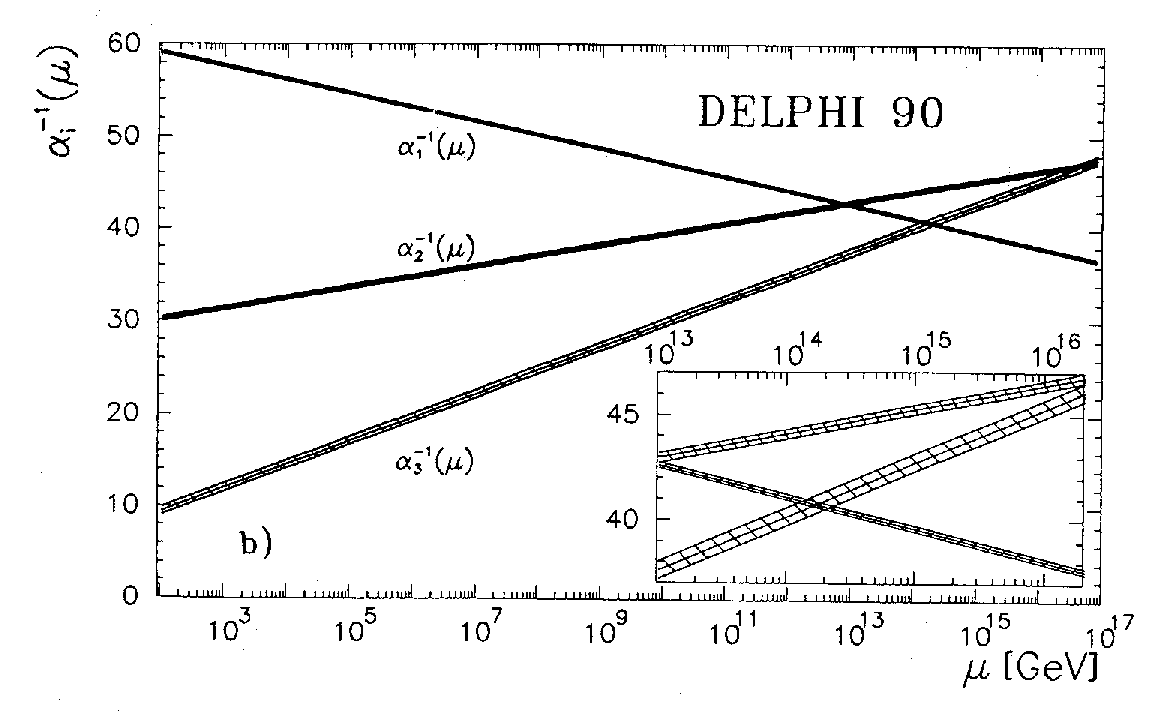
\includegraphics[width=0.49\textwidth]{figures/theory/running_couplings_SM}
      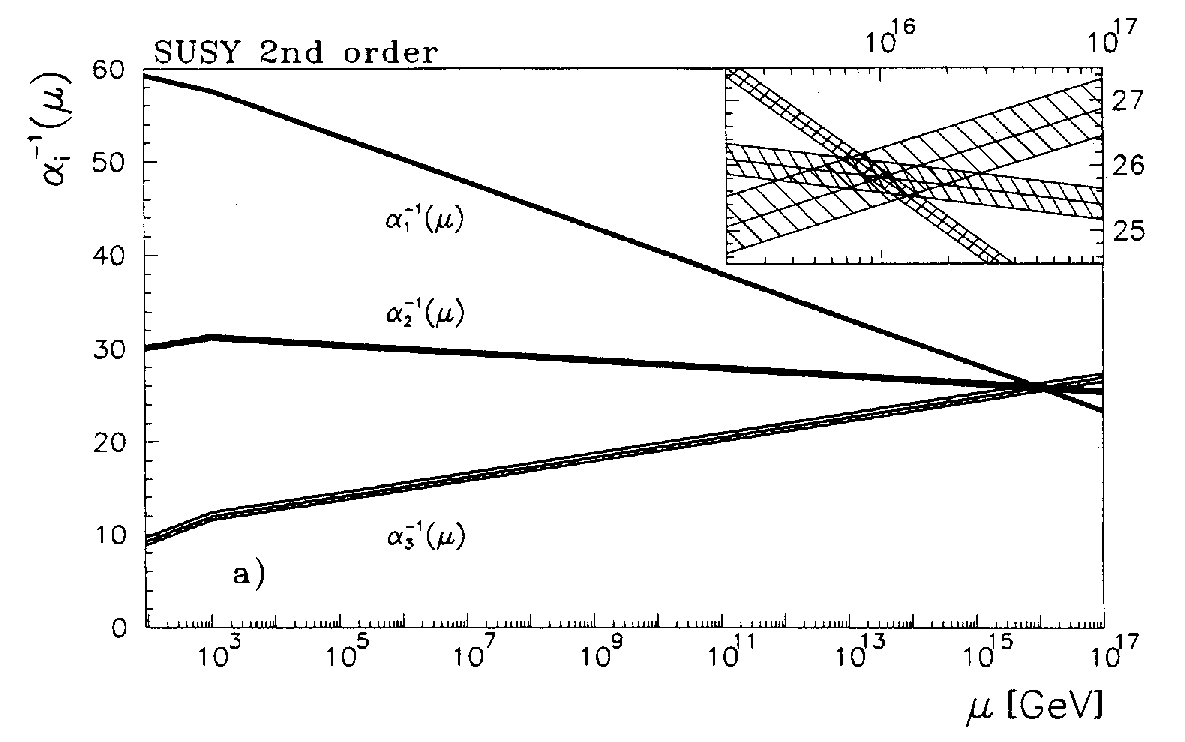
\includegraphics[width=0.49\textwidth]{figures/theory/running_couplings_MSSM}
  \caption{The running of the gauge couplings in the Standard Model (left) and in the minimal supersymmetric extension of the SM (right). Taken from~\cite{bib:Unification}.}  
  \label{fig:Unification}
\end{figure}

Besides these arguments, SUSY can also provide an answer to the problem of non-visible matter in the universe.
If the conservation of the so-called R-parity is required, the lightest supersymmetric particle (LSP) is stable.
If this particle is only weakly interacting, it can serve as a good candidate to explain fully or partially the sources of the relic density. 
R-parity is a multiplicative quantum number with 
\begin{equation}
\begin{aligned}
P_R & =  1 \qquad &&\text{SM particles}\\
P_R & = -1 &&\text{SUSY particles}.
\end{aligned}
\end{equation}
If R-parity is conserved, only terms are allowed in the Lagrangian density, that contain an even number of supersymmetric particles.
Therefore, no single SUSY particle can decay into only SM particles and thus, the LSP is stable.
The following discussions are restricted to R-parity conserving supersymmetric models.



\section{The MSSM}
\label{sec:MSSM}
The supersymmetric extension of the Standard Model with a minimal particle content is called the Minimal Supersymmetric Standard Model (MSSM).
In the following section, the particle content of the MSSM is introduced.

\subsection{The particle content of the MSSM}
In $\mathcal{N}=1$ supersymmetry, every SM particle has exactly one supersymmetric partner particle, which leads to a doubling of the particle content in the MSSM with respect to the SM\footnote{The supersymmetric partner particles of the fermions are called sfermions, whereas the partner particles of the gauge (Higgs) bosons are referred to as gauginos (higgsinos).}.
Additionally, it is necessary to introduce a second Higgs doublet to ensure the holomorphicity of the superpotential in the presence of mass terms for the up-type particles.
Furthermore, the MSSM only stays free from anomalies if there is a further Higgs doublet~\cite{bib:SUSYPrimer}.
This leads to the fact, that in the MSSM, there are five Higgs bosons instead of only one as in the SM.

\renewcommand{\arraystretch}{1.5}
\begin{table}[!b]
\centering
\caption{Chiral supermultiplets in the MSSM.}
\label{tab:chiral_multiplets}
\makebox[0.99\textwidth]{
\begin{tabular}{l|c|c|c}
\multicolumn{4}{c}{} \\
\toprule
                     &   spin 0                                     & spin $\frac{1}{2}$              & $SU(3)_C,\ SU(2)_L,\ U(1)_Y$\\ 
\midrule
   squarks/quarks    & $\left(\tilde{u}_L,\tilde{d}_L \right)$      & $\left(u_L,d_L\right)$           & $\mathbf{3},\ \mathbf{2},\ +\frac{1}{3}$\\ \cline{2-4}  
                     & $\tilde{\bar{u}}_L = \tilde{u}_R^{\dagger} $   & $\bar{u}_L = (u_R)^c$            & $\mathbf{\bar{3}},\ \mathbf{1},\ -\frac{4}{3}$\\ \cline{2-4}  
                     & $\tilde{\bar{d}}_L = \tilde{d}_R^{\dagger}$    & $\bar{d}_L = (d_R)^c$            & $\mathbf{\bar{3}},\ \mathbf{1},\ +\frac{2}{3}$\\ 
\midrule
   sleptons/leptons  & $\left(\tilde{\nu}_{eL},\tilde{e}_L\right)$   & $\left(\nu_{eL},e_L\right)$      & $\mathbf{1},\ \mathbf{2},\ -1$\\ \cline{2-4} 
                     & $\tilde{\bar{e}}_L = \tilde{e}_R^{\dagger}$    & $\bar{e}_L = (e_R)^c$            & $\mathbf{\bar{1}},\ \mathbf{1},\ +2$\\ 
\midrule
   Higgs/higgsinos   & $\left(H_u^+,H_u^0\right)$        & $\left(\tilde{H}_u^+,\tilde{H}_u^0\right)$   & $\mathbf{1},\ \mathbf{2},\ +1$\\ \cline{2-4}
                     & $\left(H_d^0,H_d^-\right)$        & $\left(\tilde{H}_d^0,\tilde{H}_d^-\right)$   & $\mathbf{1},\ \mathbf{2},\ -1$ \\ 
\bottomrule
\multicolumn{4}{c}{} 
\end{tabular}}
\end{table}  
\renewcommand{\arraystretch}{1.5}
\begin{table}[!b]
\centering
\caption{Vector supermultiplets in the MSSM.}
\label{tab:vector_multiplets}
\makebox[0.99\textwidth]{
\begin{tabular}{l|c|c|c}
\multicolumn{4}{c}{} \\
\toprule
                      &   spin $\frac{1}{2}$                                  & spin 1                 & $SU(3)_C,\ SU(2)_L,\ U(1)_Y$\\ 
\midrule
   gluinos/gluons     & $\tilde{g}$                       & $g$                 & $\mathbf{8},\ \mathbf{1},\ 0$\\ 
\midrule
   winos/$W$-bosons   & $\tilde{W}^{\pm},\ \tilde{W}^0$  & $W^{\pm},\ W^0$     & $\mathbf{1},\ \mathbf{3},\ 0$\\
\midrule
   bino/$B$-boson     & $\tilde{B}$                      & $B$                 & $\mathbf{1},\ \mathbf{1},\ 0$ \\  
\bottomrule
\multicolumn{4}{c}{}
\end{tabular}}
\end{table} 
In supersymmetry, all particles and their partner particles are described by so-called supermultiplets.
Since the generators of the gauge group commute with the generators of supersymmetry, all particles within one supermultiplet have same quantum numbers, besides the spin.
In a renormalisable theory, there are two different types of supermultiplets: chiral multiplets, which contain a two-component Weyl spinor describing the fermionic degrees of freedom and a complex scalar field for the bosonic degrees of freedom; vector multiplets containing a vector field and a two-component Weyl spinor.
The complete particle content of the MSSM is depicted in Tables~\ref{tab:chiral_multiplets} and~\ref{tab:vector_multiplets}. 
Since in supersymmetric theories only left-handed Weyl spinors appear in the Lagrangian density, the right-handed particles are described as charge conjugated spinors of the left-handed spinors.





\subsection{The Lagrangian density of the MSSM}
\label{sec:Lagrange_MSSM}
In the following, only the most important parts of the MSSM Lagrangian density will be described.
For a complete description of the Lagrangian density, the reader is again referred to~\cite{bib:Drees_2004}.

\subsubsection*{The superpotential}
The superpotential of the MSSM contains the self interaction terms of the Higgs bosons and generates the interaction terms of the Higgs bosons with the fermions and their superpartners.
As already noted, it is very common to assume R-parity conservation.
Hence, no terms appear in the Lagrangian that would violate lepton or baryon number conservation and the lightest supersymmetric particle is stable.
Thus, all possible terms are
\begin{equation}
\label{eq:SPMSSM}
 W_{\text{MSSM}} = \mu H_u \cdot H_d - Y_u^{ij} H_u \cdot Q_L^i u_R^{c\,j} + Y_d^{ij} H_d \cdot Q_L^i d_R^{\,c\,j} + Y_e^{ij} H_d \cdot L_L^i e_R^{c\,j},
\end{equation}
with the dot product defined as in~\cite{bib:Aitchison_2005} 
\begin{equation}
 A \cdot B = \epsilon^{\alpha\beta} A_{\alpha} B_{\beta} = A_1 B_2 - A_2 B_1.
\end{equation}

\subsubsection*{The soft-breaking Lagrangian density}
Since supersymmetry is broken, explicit SUSY breaking terms are added to the Lagrangian density.
In order not to introduce new sources of quadratic divergencies, only bilinear and trilinear terms appear in the soft-breaking Lagrangian
\begin{equation}
 \begin{split}
  - \mathcal{L}^{MSSM}_{soft} =\,& m_{H_u}^2 H_u^{\dagger} \cdot H_u +m_{H_d}^2 H_d^{\dagger} \cdot H_d + \left(B\mu\, H_u \cdot H_d + h.c.\right) \\
  & + m_{\tilde{Q}\,ij}^2 \tilde{Q}_{L\,i}^{\dagger} \cdot \tilde{Q}_{L\,j}+ m_{\tilde{u}\,ij}^2 \tilde{u}_{R\,i}^{c\,\dagger} \cdot \tilde{u}_{R\,j}^c
+ m_{\tilde{d}\,ij}^2 \tilde{d}_{R\,i}^{\,c\,\dagger} \cdot \tilde{d}_{R\,j}^{\,c}\\
& + m_{\tilde{L}\,ij}^2 \tilde{L}_{L\,i}^{\dagger} \cdot \tilde{L}_{L\,j}+ m_{\tilde{e}\,ij}^2 \tilde{e}_{R\,i}^{\,c\,\dagger} \cdot \tilde{e}_{R\,j}^{\,c}\\
& +\left(- \left( A_u Y_u \right)_{ij} H_u \cdot \tilde{Q}_{L\,i} \tilde{u}_{R\,j}^c +\left( A_d Y_d \right)_{ij} H_d \cdot \tilde{Q}_{L\,i} \tilde{d}_{R\,j}^{\,c} \right.\\
& \left. +\left( A_e Y_e \right)_{ij} H_d \cdot \tilde{L}_{L\,i} \tilde{e}_{R\,j}^{\,c} + h.c. \right)\\
& + \left(M_1 \tilde{B} \tilde{B} + M_2 \tilde{W}_a \tilde{W}_a + M_3 \tilde{g}_i \tilde{g}_i + h.c \right)
 \end{split}
\label{eq:SoftTerms}
\end{equation}
The first line contains mass terms for the Higgs bosons, the second and third line for the sfermions.
In the fourth and fifth line the trilinear couplings between the Higgs bosons and the sfermions appear.
Finally, the last line gives rise to mass terms for the gauginos (gluinos, winos, bino).

Because of the soft-breaking terms, the MSSM contains more than 100 free parameters.
Constraining the MSSM is thus a difficult task and usually in experimental particle physics, constrained versions of the MSSM or assumptions at the GUT scale are used to report the impact of searches on SUSY. 
In the following a short introduction of the phenomenological MSSM is given.
With its reduced parameter space, it allows to elaborate on long-lived particles in the MSSM in a much easier way.

\subsection{The phenomenological MSSM}
\label{subsec:pMSSM}
The phenomenological MSSM (pMSSM) imposes constraints that are reasonable in the sense that the pMSSM fulfils current observations and still keeps the phenomenological variety of the MSSM~\cite{bib:pMSSM}.
The following assumptions are imposed (in~\cite{bib:pMSSM} more detailed information about these assumptions can be found):
\begin{itemize}
\item No new sources of CP violation,
\item No flavour changing neutral currents,
\item First and second generation universality.
\end{itemize}
These assumption reduce the number of SUSY parameters to only 19.
The remaining free parameters are the following:
\begin{itemize}
\item $\tan \beta$ (the ratio of the vacuum expectation values of the two Higgs doublets)
\item $M_A$ (the mass of the pseudo-scalar Higgs boson)  
\item $\mu$ (the Higgs mass parameter)
\item $M_1$,$M_2$,$M_3$ (bino, wino and gluino mass parameters, respectively)
\item $m_{\tilde{q}}$, $m_{\tilde{l}}$, $m_{\tilde{u}}$, $m_{\tilde{d}}$ and $m_{\tilde{e}}$ (the first and second generation mass parameters)
\item  $m_{\tilde{Q}}$, $m_{\tilde{L}}$, $m_{\tilde{t}}$, $m_{\tilde{b}}$ and $m_{\tilde{\tau}}$ (the third generation mass parameters)
\item $A_t$, $A_b$ and $A_{\tau}$ (third generation trilinear couplings).
\end{itemize}

\section{Supersymmetry breaking}
As already noted, the mechanism of supersymmetry breaking is unknown.
There exist, however, several ideas how to spontaneously break supersymmetry.
All mechanisms have in common that they need to happen at high energies in a hidden sector.
``Messenger'' particles are introduced which mediate the breaking to the TeV scale.
This, however, implies that supersymmetry breaking is a question of extraordinary high energies and one can parametrise the breaking by the soft breaking terms introduced in Section~\ref{sec:Lagrange_MSSM}.

The most popular breaking mediation mechanisms are gravity-mediated supersymmetry breaking~\cite{bib:GravityMediation} and gauge-mediated supersymmetry breaking~\cite{bib:GaugeMediation}.

\chapter{Long-lived particles in the MSSM}
\label{ch:Longlived_Particles}
There are various mechanisms how particles can be long-lived, such as small couplings or (almost) conserved quantum numbers.
For a comprehensive review, the reader is referred to~\cite{bib:LonglivedParticles_Overview}.

In this thesis, the focus is set on particles that have a long lifetime due to a small decay phase space. 
A phase space suppression is possible when the mass splitting between the decaying particle and one of the decay products is very small.
In Part~\ref{part:analysis}, a search for highly ionising, short tracks is presented.
This search is motivated by long-lived charginos, that are nearly mass-degenerate with the lightest supersymmetric particle, the neutralino.
The underlying mechanism of this mass-degeneracy in the MSSM will be addressed in the next paragraphs.

In the MSSM, the lightest chargino (\chipm) and the lightest neutralino (\chiO) can be almost mass-degenerate, if the wino mass parameter ($M_2$) is smaller than the bino ($M_1$) and higgsino ($\mu$) mass parameters.
This can be seen from the chargino and neutralino mass matrices.
The chargino mass matrix in the basis $\Psi^+_i= \left(-i \tilde{W}^+,\tilde{h}_u^+  \right)$ and \mbox{$\Psi^-_i= \left(-i \tilde{W}^-,\tilde{h}_d^-  \right)$} is given by 
\begin{flalign}
\label{eq:CharginoMassMatrix}
\mathcal{M}_{\Psi^{\pm}} = 
\begin{pmatrix} 
M_2    & g v_d                    \\
g v_u  & \mu                  
\end{pmatrix}.
\end{flalign} 
The mass eigenstates can be deduced with the help of orthogonal matrices $V$ and $U$, \mbox{$\chi^+_i=V_{ij}\Psi^+_j$} and \mbox{$\chi^-_i = U_{ij} \Psi^-_j$}.

The neutralino mass matrix in the basis  $\Psi_i^0= \left(-i\tilde{B},-i\tilde{W}^0,\tilde{h}_u^0,\tilde{h}_d^0\right)$ is
\begin{flalign}
\label{eq:NeutralinoMassMatrix}
\mathcal{M}_{\Psi^0} = 
\begin{pmatrix} 
M_1                     & 0                       & \frac{g'v_u}{\sqrt{2}}  & -\frac{g'v_d}{\sqrt{2}}  \\
0                       & M_2                     & -\frac{g v_u}{\sqrt{2}} & \frac{g v_d}{\sqrt{2}}   \\
\frac{g'v_u}{\sqrt{2}}  & -\frac{g v_u}{\sqrt{2}} & 0                       & -\mu                     \\
-\frac{g'v_d}{\sqrt{2}} & \frac{g v_d}{\sqrt{2}}  & -\mu                    &  0                      
\end{pmatrix}.
\end{flalign}
The mass matrix can be diagonalised with an orthogonal matrix $N$ leading to four different mass eigenstates of $\tilde{\chi}^0_i = N_{ij} \Psi_j^0  $.

It can be easily seen from the mass matrices~\eqref{eq:CharginoMassMatrix} and~\eqref{eq:NeutralinoMassMatrix}, that in first order approximation - neglecting the off-diagonal elements which are of electroweak strength - the lightest chargino and the lightest neutralino are both wino-like for $M_2 < M_1,\mu$ with a mass of $m_\chi \simeq M_2$. 
Thus, the mass difference between \chipm and \chiO is only determined by higher order corrections: radiative corrections as well as tree-level mixing with other states.\\

%The following expressions are approximate neutralino and chargino mass terms for $M_2 \mu > m_W^2 \sin 2\beta$ and $|M_2 \pm \mu|$, $|M_1 \pm \mu| \gg m_Z$ (taken from~\cite{bib:PAS:CMS:pMSSM_2013})
%\begin{align}
%\label{eq:gaugino_masses}
%\begin{split}
%m_{\tilde{B}}    &\simeq  M_1   + \frac{m_Z^2 \left( M_1 + \mu \sin 2\beta  \right) \sin^2 \theta_W}{M_1^2 - \mu^2} \\
%m_{\tilde{W}}    &\simeq  M_2   + \frac{m_Z^2 \left( M_2 + \mu \sin 2\beta  \right) \cos^2 \theta_W}{M_2^2 - \mu^2} \\
%m_{\tilde{H}_1^0} &\simeq  |\mu| + \frac{m_Z^2 \left( 1 - \sin 2\beta \right) \left( \mu + M_2 \sin^2 \theta_W + M_1 \cos^2 \theta_W \right) sqn\left(\mu \right)}{2 \left(\mu +M_2 \right)\left(\mu +M_1 \right)} \\
%m_{\tilde{H}_2^0} &\simeq  |\mu| + \frac{m_Z^2 \left( 1 + \sin 2\beta \right) \left( \mu - M_2 \sin^2 \theta_W - M_1 \cos^2 \theta_W \right) sqn\left(\mu \right)}{2 \left(\mu -M_2 \right)\left(\mu -M_1 \right)} 
%\end{split}
%\end{align}
%\begin{align}
%\label{eq:chargino_masses}
%\begin{split}
%m_{\tilde{W}^{\pm}} &\simeq  M_2  + m_W^2 \left[ \frac{M_2 + \mu \sin 2\beta}{M_2^2 - \mu^2} \right]\\
%m_{\tilde{H^{\pm}}} &\simeq  |\mu|  + m_W^2 sgn\left( \mu \right) \left[ \frac{\mu + M_2 \sin 2\beta}{\mu^2 - M_2^2} \right]
%\end{split}
%\end{align}
%It is obvious from Eqs.~\ref{eq:gaugino_masses} and~\ref{eq:chargino_masses}, that if $M_2 < M_1,\, |\mu|$, the lightest neutralino state is wino-like and is fully mass-degenerate on tree level with the lightest chargino.


Furthermore, recent analyses of the pMSSM parameter space~\cite{bib:pMSSMScan_2013,bib:pMSSMScan_2012} show, that models with almost pure wino-like neutralinos as LSPs mostly come along with wino-like charginos being the next-to lightest supersymmetric particle (NLSP).
In~\cite{bib:pMSSMScan_2013}, a parameter scan in the pMSSM parameter space is performed, flat in the 19 different SUSY parameters.
Afterwards, the generated 3 million pMSSM models are confronted with theoretical constraints as well as experimental observations.
Theoretical constraints are \eg requiring stable vacua and no colour- or charge breaking minima.
Furthermore, the agreement with precision electroweak data, heavy flavour physics and collider results from LEP, Tevatron and LHC is required.
The accordance with relic density data is only implemented as an upper bound.
Phenomenological MSSM models that survive these constraints and have a wino-like neutralino as lightest supersymmetric particle, do frequently contain  a metastable chargino.
In a fraction of $\sim 25\%$ of these models, the metastable chargino decays inside the tracker, calorimeter or muon chamber.
The mass splitting between chargino and neutralino in these scenarios is typically of the order of $\sim160\mev$~\cite{bib:pMSSMScan_2013}.

Furthermore, a study has been performed within~\cite{bib:CMS:DT_8TeV} which interpretes the results of various beyond Standard Model searches in terms of the fraction of excluded parameter points in the pMSSM.
This study shows, that lifetimes between $1\cm \lesssim c\tau \lesssim 30\cm$ could not yet been accessed by any of the existing searches (cf. Fig.~\ref{fig:pMSSMplot} in Section~\ref{sec:Motivation}).



\section{Previous searches and constraints from indirect searches}

Several previous searches are sensitive on SUSY scenarios with almost mass-degenerate wino-like charginos and neutralinos.
In the following an overview about these previous searches will be given.

\subsection*{Searches at LEP}
Several searches at LEP were hunting for almost mass-degenerate neutralino-chargino scenarios~\cite{bib:PreviousSearches_ALEPH,bib:PreviousSearches_OPAL,bib:PreviousSearches_DELPHI_2003,bib:PreviousSearches_DELPHI}.
These searches were looking for events with a high-energetic initial state radiated photon leading to missing energy in events with chargino-pair production and invisible decay products.
The excluded parameter regions by these searches can be found in~\cite{bib:LEP:SUSY_results} and are depicted in Fig.~\ref{fig:LEP}.
The searches were interpreted for $M_1$ and $M_2$ almost degenerate and with a large unified scalar mass $m_0$ leading to sneutrino masses larger than 500\gev. 
Charginos are excluded up to a mass of 92.4\gev~\cite{bib:LEP:SUSY_results}.
\begin{figure}[!h]
  \centering
      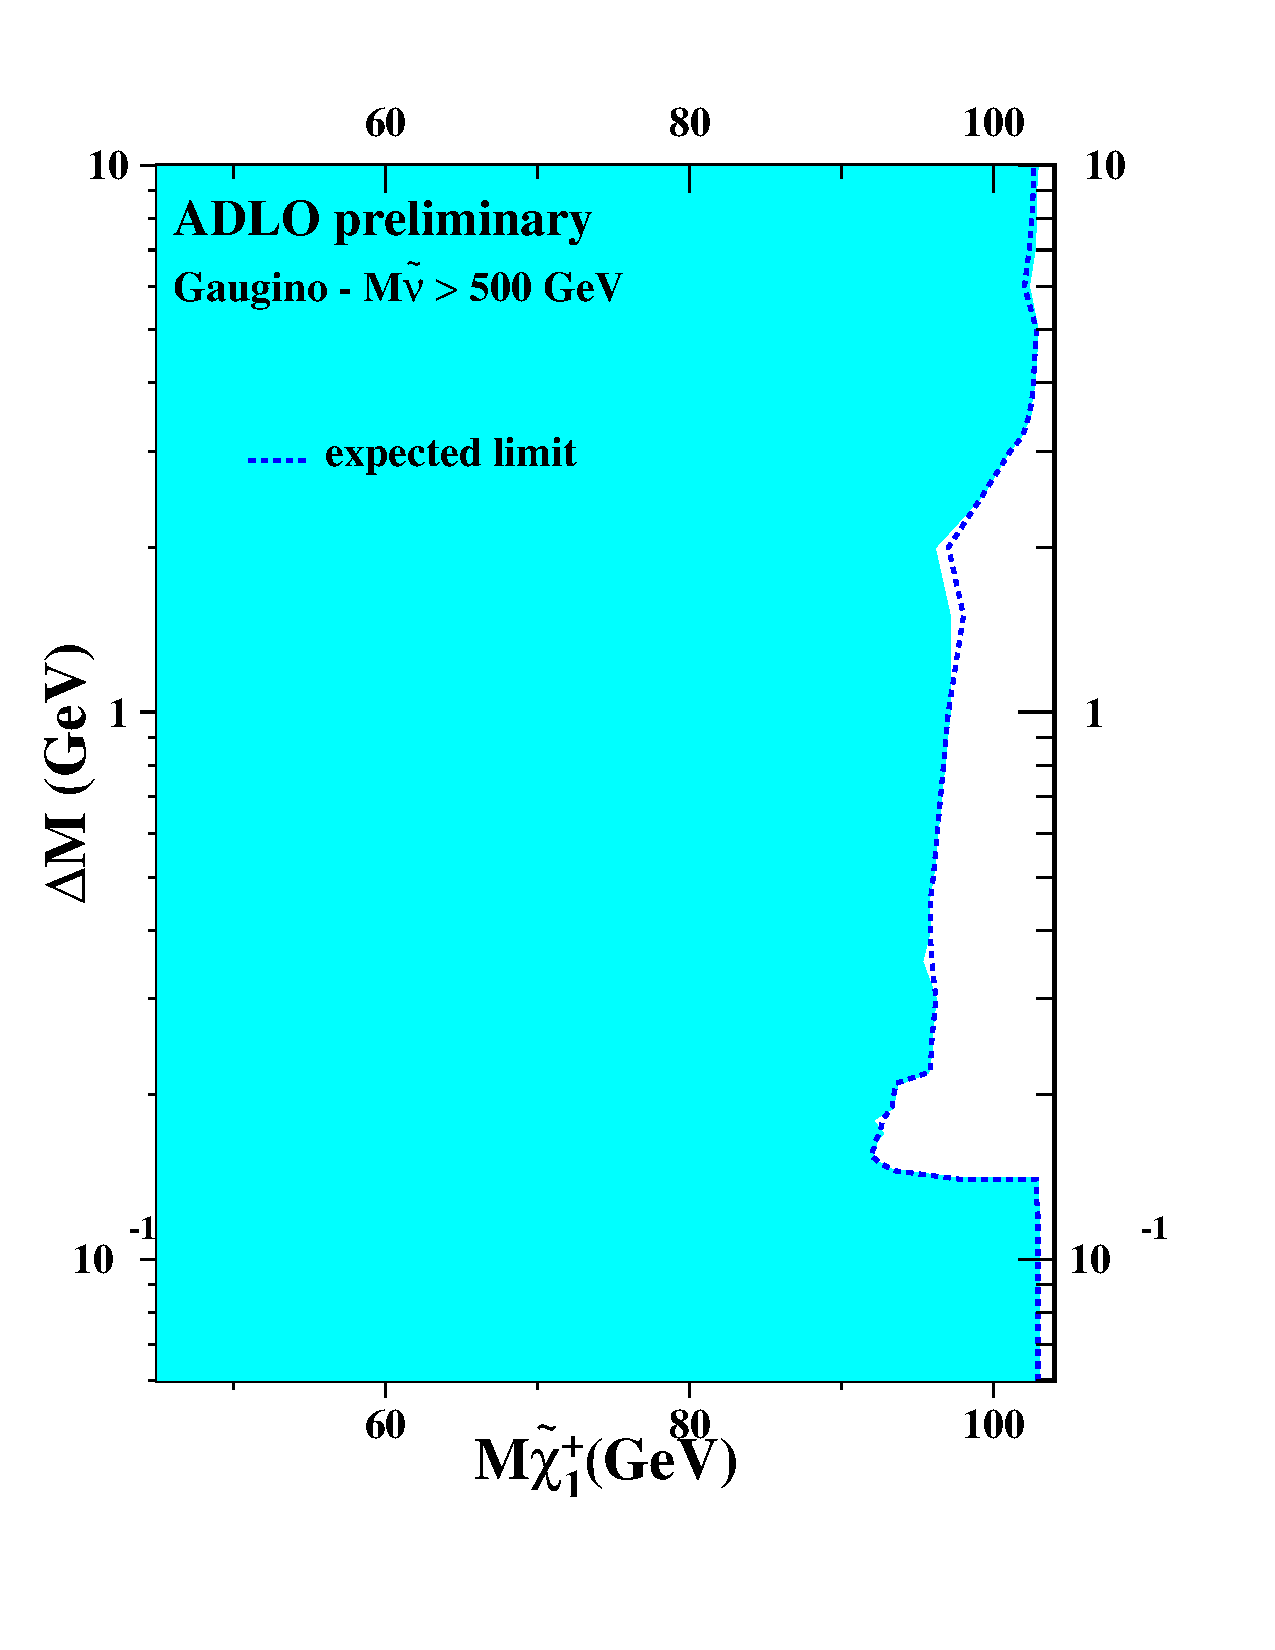
\includegraphics[width=0.45\textwidth]{figures/theory/mass_adlo_gaug_1.pdf}
  \caption{Observed and expected exclusion limits by LEP searches in the $m_{\chipm}-\Delta m \left( \chipm, \chiO \right)$ plane for almost degenerate $M_1$ and $M_2$ and a large unified scalar mass $m_0$. Taken from~\cite{bib:LEP:SUSY_results}.}  
  \label{fig:LEP}
\end{figure}

\subsection*{Searches at ATLAS at 7 and 8\tev}
At the ATLAS experiment at the LHC, searches for events with a disappearing track signature were performed at $\sqrt{s}=7\tev$~\cite{bib:PreviousSearches_Atlas_DT_7TeV} as well as at $\sqrt{s}=8\tev$~\cite{bib:PreviousSearches_Atlas_DT_8TeV}. 
Furthermore, a search for metastable particles with high ionisation losses was performed with $\sqrt{s}=8\tev$ data~\cite{bib:PreviousSearches_ATLAS_DEDX}.
These searches were interpreted within an anomaly-mediated supersymmetry breaking model~\cite{bib:Theory_AMSB_1998} with $\tan\beta=5$ and $\mu>0$.
The excluded parameter space by these searches is shown in Fig.~\ref{fig:ATLAS}.
Models with charginos down to lifetimes of 0.06\ns could be excluded.


\subsection*{Searches at CMS at 7 and 8\tev}
There are several searches at the CMS experiment at the LHC that are sensitive to long-lived wino-like charginos.
Among them is the search for long-lived charged particles~\cite{bib:CMS:HSCP_8TeV}, which searched for heavy particles with large energy deposits in the tracker at $\sqrt{s}=7\tev$  and $\sqrt{s}=8\tev$.
Furthermore, there is the search for disappearing tracks~\cite{bib:CMS:DT_8TeV} which analysed events with disappearing tracks in the tracker with respect to wino-like charginos almost mass-degenerate with the lightest neutralino.
This search was performed at the CMS experiment at a centre-of mass energy of $\sqrt{s}=8\tev$.
Since the latter search is more sensitive to shorter lifetime, only the exclusion limits derived by this search are shown in Fig.~\ref{fig:CMS}.
The disappearing track search by CMS shows a very similar sensitivity as the searches done at the ATLAS experiment.

\begin{figure}[!h]
  \centering
      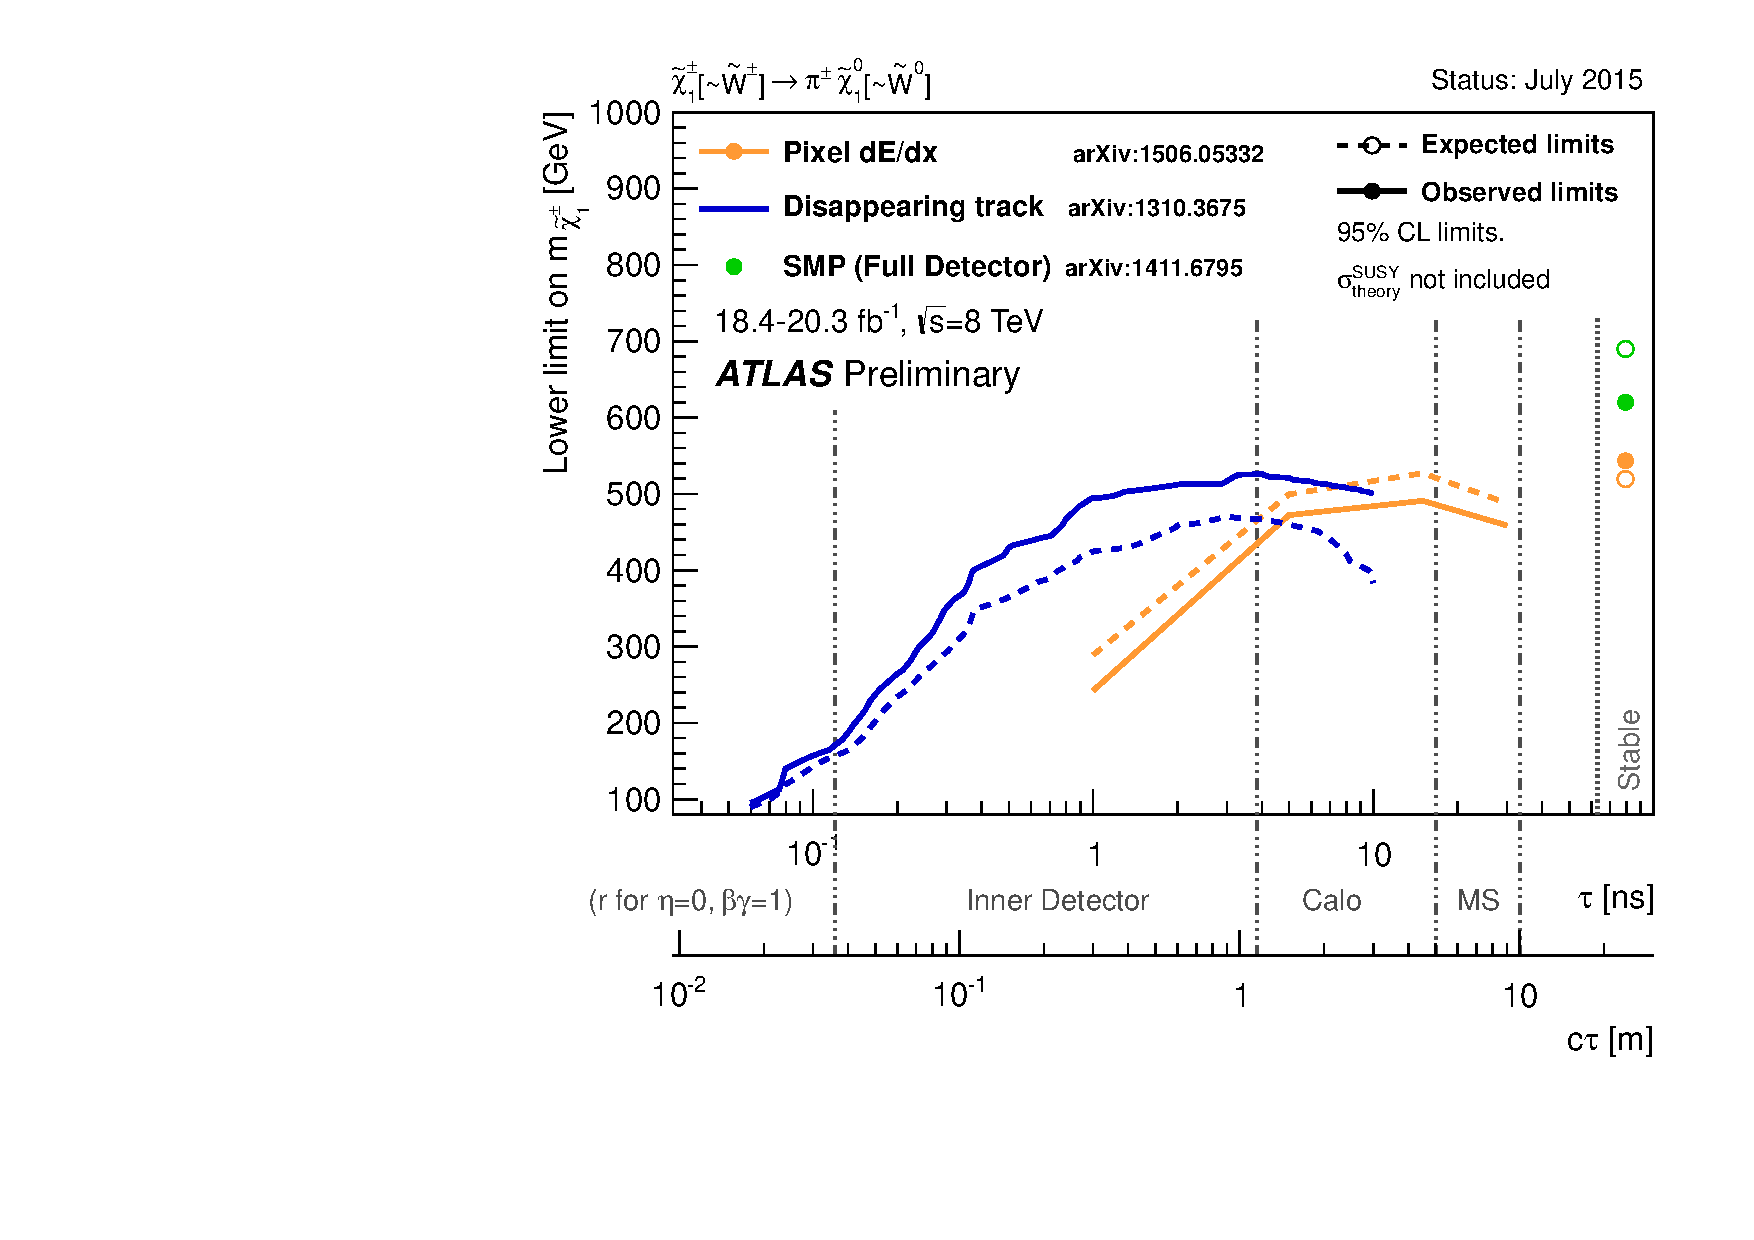
\includegraphics[width=0.54\textwidth]{figures/theory/ATLAS_SUSY_LLPChargino.pdf}
  \caption{Excluded parameter space by ATLAS searches in the $m_{\chipm}-\tau_{\chipm}$ plane for an AMSB model with $\tan\beta=5$ and $\mu>0$. Only chargino pair production is taken into account. The area below the curves is excluded. Taken from~\cite{bib:ATLAS_SUMMARYPLOTS}.}  
  \label{fig:ATLAS}
\end{figure}
\begin{figure}[!h]
  \centering
      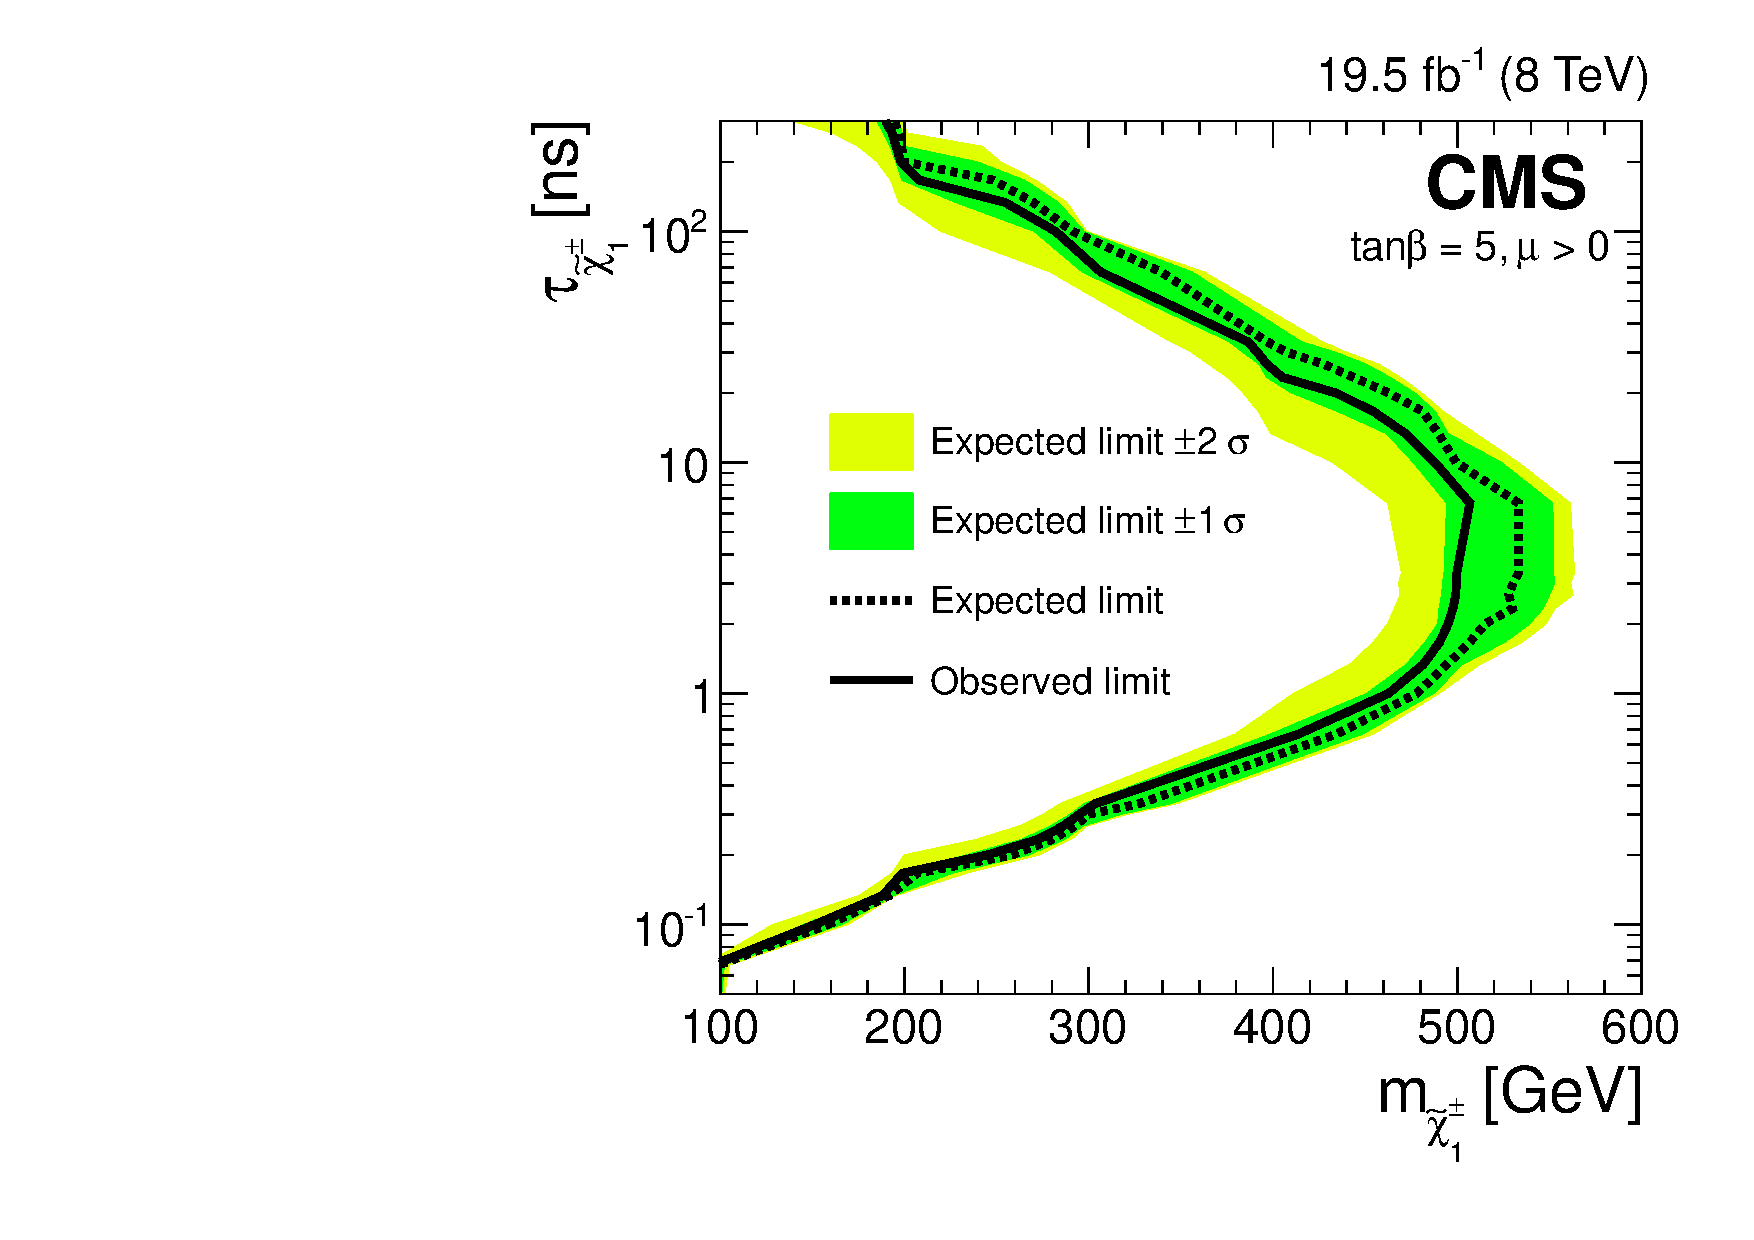
\includegraphics[width=0.54\textwidth]{figures/theory/lifetimeNs_vs_mass.pdf}
  \caption{Excluded parameter space by the Disappearing track search of CMS in the $\tau_{\chipm}-m_{\chipm}$ plane for wino-like charginos. The region left to the curve is excluded. Taken from~\cite{bib:CMS:DT_8TeV}.}  
  \label{fig:CMS}
\end{figure}

\subsection*{Indirect searches}
Finally, also results from indirect dark matter searches constrain the parameter region of SUSY models with wino-like charginos and neutralinos.
The most stringent limits are due to results by the Fermi Gamma-Ray Space Telescope (Fermi)~\cite{bib:Fermi} and the High Energy Spectroscopic System (H.E.S.S.)~\cite{bib:HESS}.

By the comparison of the observed gamma-ray signal to the theoretical prediction, Fermi sets upper limits on the dark matter annihilation cross-section considering six different decay channels~\cite{bib:Fermi_DM}.

H.E.S.S. sets upper limits on the DM annihilation cross section by the observation of the $\gamma$-ray line which is expected near the DM mass~\cite{bib:HESS_DM}.

Recent interpretations of the Fermi and H.E.S.S. data~\cite{bib:IndirectSearches_Fan_2013,bib:IndirectSearches_Cohen_2013,bib:IndirectSearches_Hryczuk_2014,bib:IndirectSearches_Beneke_2015} show that thermally produced wino-like neutralinos can only account for the full relic density for $\sim3.1\tev$~\cite{bib:IndirectSearches_Cohen_2013}, while DM masses between $1.6-3.0\tev$ are excluded by Fermi and H.E.S.S. observations.
Lower masses are still allowed, however, the neutralino cannot make up the full relic density.
%For scenarios with non-thermally produced neutralinos, the full mass region up to 3.1\tev is ruled out for scenarios where the wino-like neutralino is the only source of dark matter~\cite{bib:IndirectSearches_Cohen_2013}. 




% \part{Experimental setup/ Experiment and ... Experimental Setup: Collider, detector and algorithms } \label{part:Detector}
% \part{Experimental setup/ Experiment and ... Experimental Setup: Collider, detector and algorithms } \label{part:Detector}
\part{Experimental setup: Collider, detector and algorithms } \label{part:Experiment}
%%%%%%%%%%%%%%%%%%%%%%%%%%%%%%%%%%%%%%%%%%%%%%%%%%%%%%%%%%%%%%%%%%%%%%%%%%%%%%%%%%%%%%%%%%%%%%%%%%%%%%%%%%%%%%%%%%%%%%%%%%%%%%%%%%%%%%%%%%%%%%%%%%%%%%%%%%%%%%%%%%%%%%%%%%%%%%%%%%%%%%%%%%%%%%%%%%%%%%%%%%%%%%%%%%%%%%%%%%%%%%%%%%%
%%%%%%%%%%%%%%%%%%%%%%%%%%%%%%%%%%%%%%%%%%%%%%%%%%%%%%%%%%%%%%%%%%%%%%%%%%%%%%%%%%%%%%%%%%%%%%%%%%%%%%%%%%%%%%%%%%%%%%%%%%%%%%%%%%%%%%%%%%%%%%%%%%%%%%%%%%%%%%%%%%%%%%%%%%%%%%%%%%%%%%%%%%%%%%%%%%%%%%%%%%%%%%%%%%%%%%%%%%%%%%%%%%%
%%%%%%%%%%%%%%%%%%%%%%%%%%%%%%%%%%%%%%%%%%%%%%%%%%%%%%%%%%%%%%%%%%%%%%%%%%%%%%%%%%%%%%%%%%%%%%%%%%%%%%%%%%%%%%%%%%%%%%%%%%%%%%%%%%%%%%%%%%%%%%%%%%%%%%%%%%%%%%%%%%%%%%%%%%%%%%%%%%%%%%%%%%%%%%%%%%%%%%%%%%%%%%%%%%%%%%%%%%%%%%%%%%%
\chapter{The Large Hadron Collider}

The Large Hadron Collider (LHC)~\cite{bib:LHC_machine_2008,bib:LHC_2004} is a particle accelerator installed in the former LEP~\cite{bib:LEP_design_1984} tunnel at CERN~\cite{bib:CERN:web}.
It is 26.7\km in circumference and consists of two separate rings, which are, in periods of operation, inhabited by two counter-circulating beams.
At the interaction points of the two beams, either proton-proton collisions or heavy ion collisions take place.
In this thesis, only $pp$-collision data from the year 2012 is analysed.
Thus, all machine values cited in the following chapters and paragraphs refer to the setup for $pp$-collisions in 2012 if not stated otherwise.

The beams are separated into bunches which rotate with a bunch spacing of 50\ns corresponding to a collision frequency of 20\mhz.
Before the bunches are actually filled into the LHC ring they are pre-accelerated in other accelerators, which are in the order they are actually passed by the protons: Linac2, Proton  Synchrotron Booster (PSB), Proton Synchrotron (PS), Super Proton Synchrotron (SPS).
The injector chain and the LHC ring with its experiments is visualised in Fig~\ref{fig:LHC}.
\begin{figure}[!b]
  \centering
      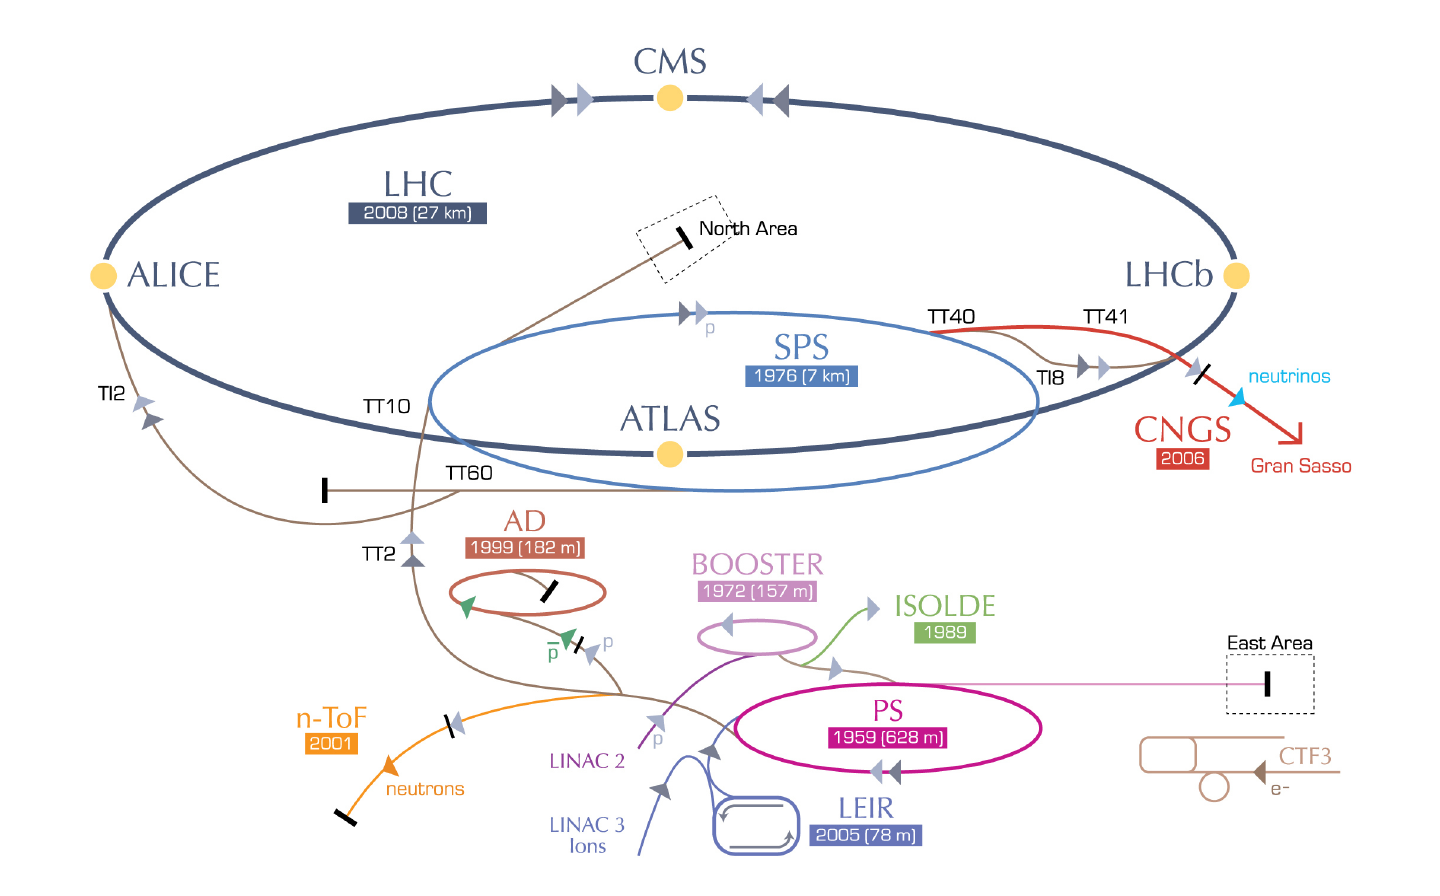
\includegraphics[width=0.90\textwidth]{figures/experiment/LHC/LHC_small.png}
  \caption{Visualisation of the LHC with its experiments and the injector chain. Taken from~\cite{bib:CERNBrochure}.}  
  \label{fig:LHC}
\end{figure}

In the LHC, the beams are kept on their circular path with the help of a magnetic field of 4.76\tesla.
Further quadrupole and sextupole magnets squeeze and focus the bunches resulting in a bunch spread of roughly 8\cm length and a Gaussian shape radius of 20\mum RMS at the interaction point.
The number of protons contained in each bunch is of the order $10^{11}$.
The LHC hosts four main particle physics experiments: the CMS, ATLAS, LHCb and ALICE experiments.
CMS~\cite{bib:CMS:experiment,bib:CMS:TDR} and ATLAS~\cite{bib:ATLAS:experiment,bib:ATLAS:TDR_1,bib:ATLAS:TDR_2} are so-called ``general purpose experiments'', that are used for a variety of different physics analyses.
In contrast, the LHCb~\cite{bib:LHCb:experiment} and ALICE~\cite{bib:ALICE:experiment} experiments are designed with an emphasis on CP-violation measurements and heavy ion collisions, respectively.
Each experiment is thus interested in different processes that happen at the beam collision points.

The number of expected events for a given process can be expressed in terms of the corresponding cross section $\sigma$ times the integrated luminosity
\begin{equation}
N = L \cdot \sigma,
\end{equation}
with an integrated luminosity of $L=\int \mathcal{L}\, dt$, where $\mathcal{L}$ is the instantaneous luminosity.
The instantaneous luminosity $\mathcal{L}$ depends on several machine parameters, such as the collision frequency $f$, the number of particles in the bunches $n_1$ and $n_2$,
the spread in the transverse plane of the bunches $\sigma_x$ and $\sigma_y$, and a geometrical correction parameter $F$ due to the crossing angle of the two bunches at the interaction point:
\begin{equation}
\mathcal{L} = \frac{f n_1 n_2 }{4 \pi \sigma_x \sigma_y} \cdot F.
\end{equation}
In 2012, the peak luminosity was $7.7 \cdot 10^{33} \frac{1}{\text{cm}^2\,\text{s}}$.
The total integrated luminosity of $pp$-collisions over time recorded at the CMS experiment is shown in Fig.~\ref{fig:Lumi}.
\begin{figure}[!b]
  \centering
      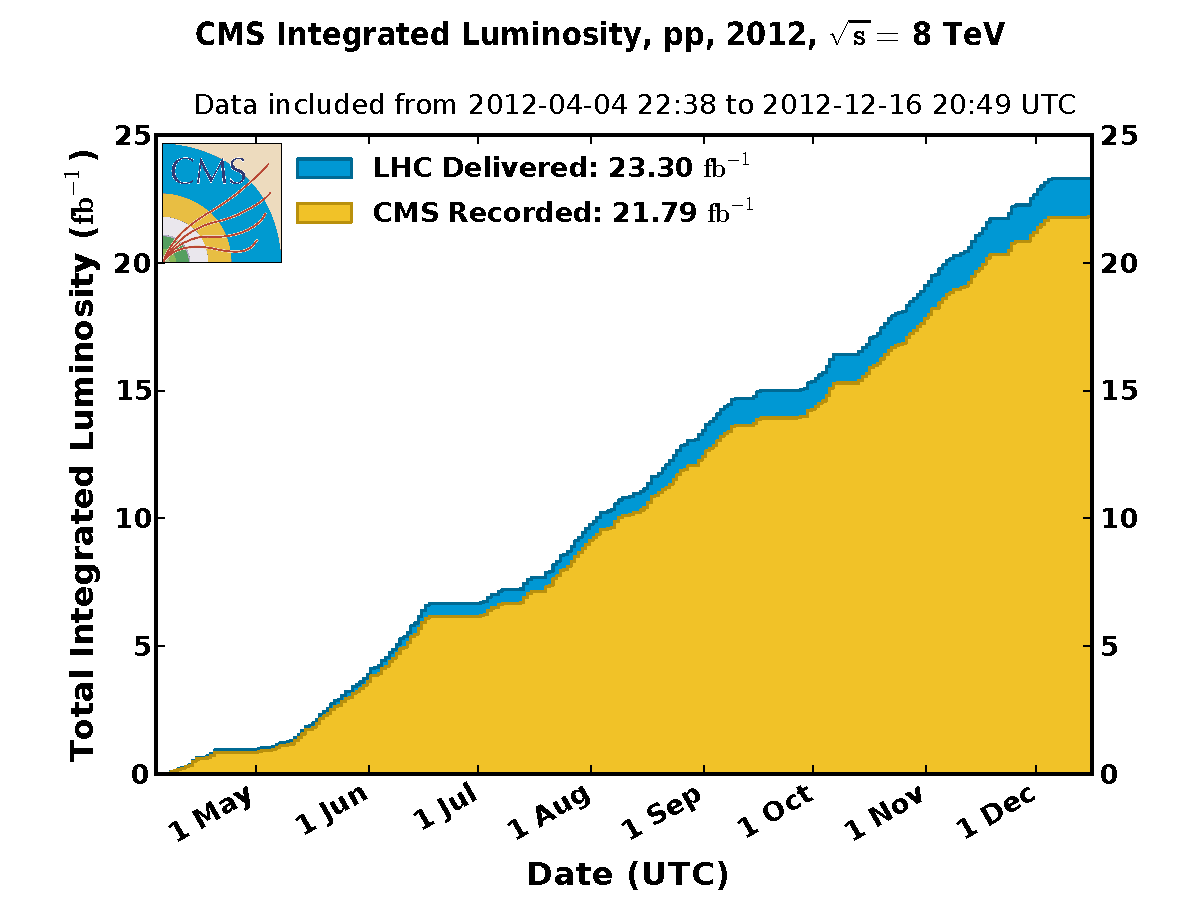
\includegraphics[width=0.55\textwidth]{figures/experiment/LHC/int_lumi_per_day_cumulative_pp_2012.pdf}
  \caption{Integrated luminosity delivered by LHC (blue) and recorded by CMS (orange) in the year 2012. Taken from~\cite{bib:LumiWiki}.}  
  \label{fig:Lumi}
\end{figure}

%%%%%%%%%%%%%%%%%%%%%%%%%%%%%%%%%%%%%%%%%%%%%%%%%%%%%%%%%%%%%%%%%%%%%%%%%%%%%%%%%%%%%%%%%%%%%%%%%%%%%%%%%%%%%%%%%%%%%%%%%%%%%%%%%%%%%%%%%%%%%%%%%%%%%%%%%%%%%%%%%%%%%%%%%%%%%%%%%%%%%%%%%%%%%%%%%%%%%%%%%%%%%%%%%%%%%%%%%%%%%%%%%%%
%%%%%%%%%%%%%%%%%%%%%%%%%%%%%%%%%%%%%%%%%%%%%%%%%%%%%%%%%%%%%%%%%%%%%%%%%%%%%%%%%%%%%%%%%%%%%%%%%%%%%%%%%%%%%%%%%%%%%%%%%%%%%%%%%%%%%%%%%%%%%%%%%%%%%%%%%%%%%%%%%%%%%%%%%%%%%%%%%%%%%%%%%%%%%%%%%%%%%%%%%%%%%%%%%%%%%%%%%%%%%%%%%%%
%%%%%%%%%%%%%%%%%%%%%%%%%%%%%%%%%%%%%%%%%%%%%%%%%%%%%%%%%%%%%%%%%%%%%%%%%%%%%%%%%%%%%%%%%%%%%%%%%%%%%%%%%%%%%%%%%%%%%%%%%%%%%%%%%%%%%%%%%%%%%%%%%%%%%%%%%%%%%%%%%%%%%%%%%%%%%%%%%%%%%%%%%%%%%%%%%%%%%%%%%%%%%%%%%%%%%%%%%%%%%%%%%%%
\FloatBarrier
\chapter{The CMS detector}
The Compact Muon Solenoid (CMS) detector~\cite{bib:CMS:experiment,bib:CMS:TDR} is a general purpose detector, designed to explore particle physics phenomena up to the multi-TeV scale.
The detector concept is an onion-like structure of different layers, each one made up of a different type of detector. 
The CMS detector measures 21.6\m in length and 14.6\m in diameter with a total weight of 12\,500\,tons.
In Fig.~\ref{fig:CMSdetector}, a perspective view of the CMS detector is depicted. 
\begin{figure}[!b]
  \centering
      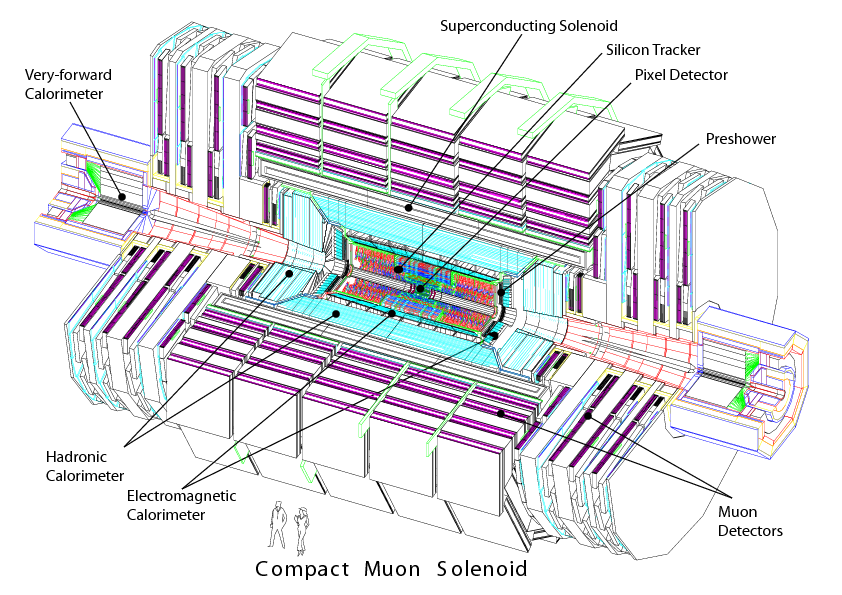
\includegraphics[width=0.89\textwidth]{figures/experiment/CMS/cms_complete_labelled.png}
  \caption{A perspective view of the CMS detector. Taken from~\cite{bib:CMS:experiment}}  
  \label{fig:CMSdetector}
\end{figure}

The coordinate system used at CMS consists of the pseudorapidity $\eta = -\ln \tan{\frac{\theta}{2}}$ and the azimuthal angle $\phi$.
The advantage of the pseudorapidity $\eta$ is the Lorentz invariance with respect to the z-axis (beam axis).
The angle $\phi$ covers the direction in the $x-y$ plane (orthogonal to the beam axis).

In order to measure the momentum of charged particles a superconducting solenoid is incorporated between the calorimeter system and the muon system providing a uniform axial magnet field of 3.8\tesla.
Iron yokes contained within the muon system ensure the return of the magnetic flux. 

In the following, the various detector components of the CMS detector from the inside to the outside as well as the trigger system will be explained.
%%%%%%%%%%%%%%%%%%%%%%%%%%%%%%%%%%%%%%%%%%%%%%%%%%%%%%%%%%%%%%%%%%%%%%%%%%%%%%%%%%%%%%%%%%%%%%%%%%%%%%%%%%%%%%%%%%%%%%%%%%%%%%%%%%%%%%%%%%%%%%%%%%%%%%%%%%%%%%%%%%%%%%%%%%%%%%%%%%%%%%%%%%%%%%%%%%%%%%%%%%%%%%%%%%%%%%%%%%%%%%%%%%%
\FloatBarrier
\section{The tracking system}
The tracking detector~\cite{bib:CMS:TDR_2006,bib:CMS:Tracker_1997,bib:CMS:Tracker_2000} is the innermost detector at CMS. 
It is a silicon semiconductor detector and is included for the tasks of vertex and track reconstruction by the measurement of particles' energy losses.
A schematic sketch of the tracker at CMS is depicted in Fig.~\ref{fig:Tracker}.
\begin{figure}[!b]
  \centering
      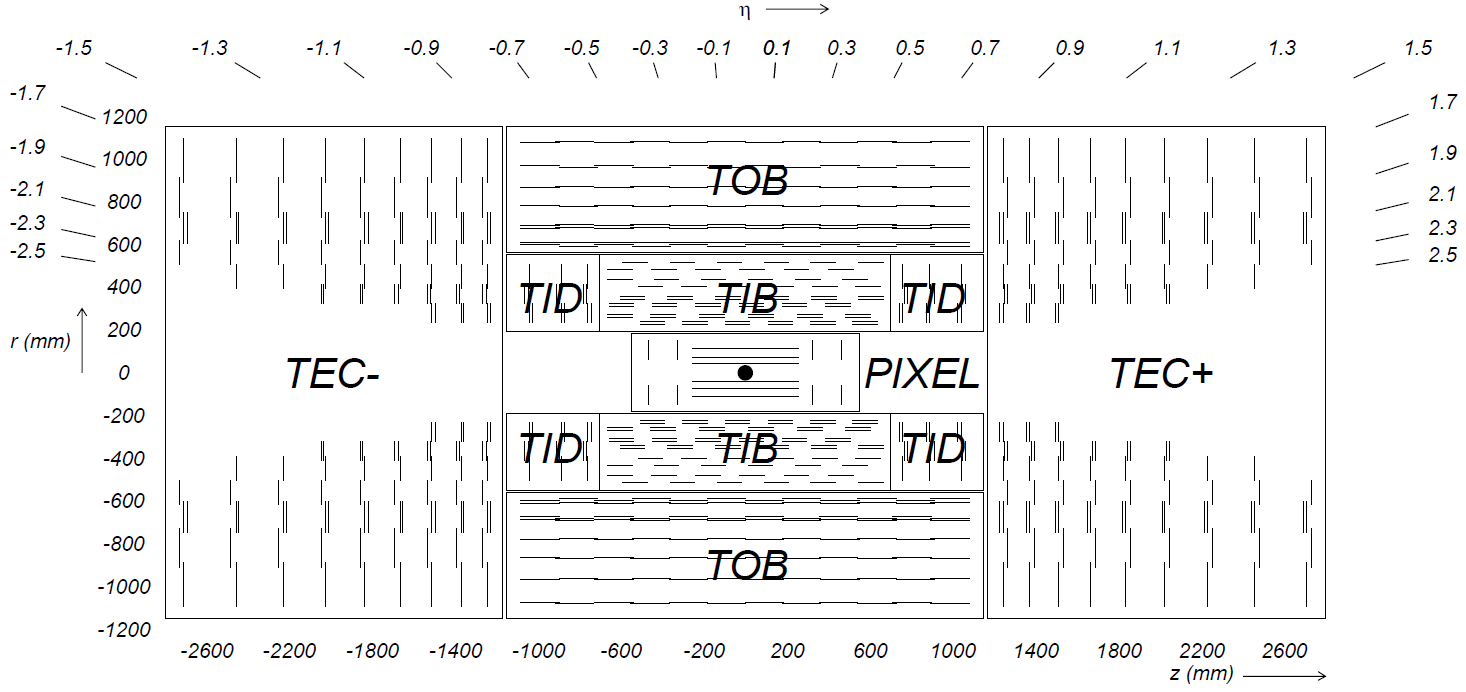
\includegraphics[width=0.99\textwidth]{figures/experiment/CMS/Figures_Experimental_Apparatus_Tracker.png}
  \caption{Schematic sketch of the silicon tracker at CMS in the $z - \phi$ plane including the silicon pixel detector (PIXEL) as well as the different components of the silicon strip detector: tracker inner barrel (TIB), tracker outer barrel (TOB), tracker endcap (TEC), and tracker inner disk (TID). Taken from~\cite{bib:CMS:tracking_8TeV}.
           }  
  \label{fig:Tracker}
\end{figure}
The tracking system is divided into two parts: the innermost tracker is a silicon pixel detector surrounded by a silicon strip detector.
Both parts will be explained in detail in the upcoming sections, followed by a short description of how the energy of a traversing particle is measured with the silicon sensors.
As a calibration of the silicon pixel detector was performed within this PhD thesis (see Section~\ref{sec:EnergyCalibration}), an emphasis will be put on the pixel detector.


%%%%%%%%%%%%%%%%%%%%%%%%%%%%%%%%%%%%%%%%%%%%%%%%%%%%%%%%%%%%%%%%%%%%%%%%%%%%%%%%%%%%%%%%%%%%%%%%%%%%%%%%%%%%%%%%%%%%%%%%%%%%%%%%%%%%%%%%%%%%%%%%%%%%%%%%%%%%%%%%%%%%%%%%%%%%%%%%%%%%%%%%%%%%%%%%%%%%%%%%%%%%%%%%%%%%%%%%%%%%%%%%%%%
\subsection*{The silicon pixel tracker}
The silicon pixel detector consists of three different cylindrical layers in the barrel region at radii of 4.4\cm, 7.3\cm and 10.2\cm and two discs in the endcaps at $z$-distances of 34.5\cm and 46.5\cm.
It is made up of 1440 modules in total (barrel + endcaps), each module comprising 8 or 16 read-out-chips (ROCs).
The read-out-chips are bump bonded~\cite{Thesis_Jenny} to a pixel system of $52\times80$ pixels, which are read out in double columns (see~\cite{Thesis_Jenny} on detailed information of the readout electronics).
A visualisation of a part of a pixel module is shown in Fig.~\ref{fig:PixelTracker}.
\begin{figure}[!b]
  \centering
      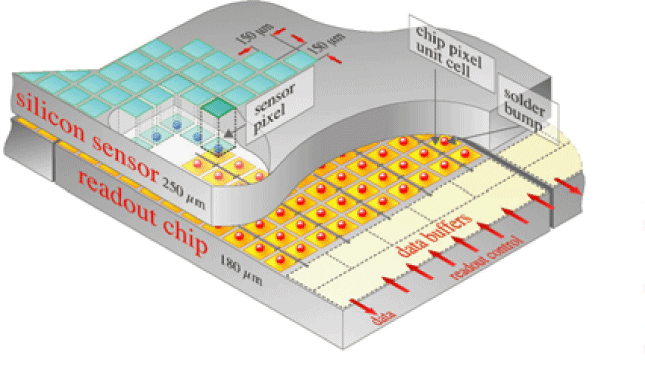
\includegraphics[width=0.90\textwidth]{figures/experiment/CMS/Pixelement.png}
  \caption{Schematic sketch of a part of a silicon pixel tracker module including the silicon sensors and the read-out-chip (ROC). Taken from~\cite{bib:CMS:tracking_8TeV}.}  
  \label{fig:PixelTracker}
\end{figure}
In total, there are 65 million pixels comprised in the pixel detector.
The large number of pixels and their small size ensure a low occupancy close to the vertex of around $0.002 - 0.02$\%~\cite{bib:CMS:tracking_8TeV} and a high hit efficiency of around 99\%~\cite{bib:CMS:PixelSpatialResolution}. 

The silicon pixel detector is very important for the reconstruction of primary and secondary vertices as well as the reconstruction of particle tracks.
Therefore, a high spatial resolution is needed.
This is achieved by the small size of the pixels ($ 150 \times 100 \mum^2$) and the exploitation of the spread of the energy deposition across several pixels (in average the energy is deposited across 3-5 pixels~\cite{bib:TWIKI:PixelClusterSize}).
Exploiting the energy spread across pixels, a spatial resolution in the barrel region of 9.4\mum in the $r - \phi$ plane and - dependent on the incident angle of a track - a hit resolution between $20-45\mum$ in the z-direction is achieved~\cite{bib:CMS:tracking_8TeV}. 
%The high spatial resolution makes the pixel detector perfectly suited for the reconstruction of vertices and tracks.
The spatial resolution of the primary vertex depends on the number of tracks taken into account for the reconstruction of the primary vertex.
For more than 50 tracks originating from the primary vertex the spatial resolution is around $10-12\mum$ for each of the three spatial dimensions~\cite{bib:CMS:tracking_8TeV}.
The reconstruction efficiency of primary vertices is close to 100\% if more than two tracks are used for the vertex reconstruction~\cite{bib:CMS:tracking_8TeV}.

\subsection*{The silicon strip tracker}
The silicon strip tracker is the next-to innermost detector of the CMS detector and ranges up to a radius of 1.1\m.
The barrel region consists of a tracker inner barrel (TIB) and a tracker outer barrel (TOB).
The TIB has four layers with two layers equipped with stereo modules to measure the hit position additionally in the $r-z$ plane.
The silicon sensors in the TIB are of 320\mum thickness with a strip pitch varying between $80-120\mum$.
The TOB has six different layers (two layers of stereo modules) with silicon sensors of 500\mum thickness and strip pitches between 120 and 180\mum. 

The endcaps are subdivided into a tracker endcap (TEC) and a tracker inner disk (TID).
They ensure a coverage of a pseudorapidity up to $|\eta|=2.5$.
In each TEC, 9 disks between a z-position of $120\cm < z < 280\cm$ are contained.
Each of the TID comprises three disks between $60\cm < z < 110\cm$.

In the barrel region, a single-point resolution between $23 - 52\mum$ in the $r-\phi$ plane and $230 - 530\mum$  in the z-direction is achieved.
%FIXME: What about momentum resolution

\subsection*{Energy measurements in the tracking system}
A charged particle traversing the above mentioned silicon detectors produces electron-hole pairs in the semiconducting material along its trajectory, thus loosing energy due to ionisation.
For silicon, the mean energy to create an electron-hole pair is 3.61\ev at $-10\degree$C.
Minimally ionising particles produce an average of 22\,000 electron-hole pairs in silicon sensors~\cite{Thesis_Jenny}.
Electrons that are subject to a hard collision with the incoming particle (so-called delta-rays), produce further ionisation and can thus lead to much higher energy deposits in the silicon.
Because of the applied bias voltage at the sensors (for the creation of a depletion zone), the released electrons (holes) travel to the n-contacts (p-contacts), thereby inducing a current which is measured by the readout electronics. 
A more detailed description of the energy measurement in silicon sensors can be found in~\cite{Thesis_Jenny}.

%%%%%%%%%%%%%%%%%%%%%%%%%%%%%%%%%%%%%%%%%%%%%%%%%%%%%%%%%%%%%%%%%%%%%%%%%%%%%%%%%%%%%%%%%%%%%%%%%%%%%%%%%%%%%%%%%%%%%%%%%%%%%%%%%%%%%%%%%%%%%%%%%%%%%%%%%%%%%%%%%%%%%%%%%%%%%%%%%%%%%%%%%%%%%%%%%%%%%%%%%%%%%%%%%%%%%%%%%%%%%%%%%%%
\section{The electromagnetic calorimeter}
The electromagnetic calorimeter (ECAL)~\cite{bib:CMS:TDR_2006,bib:CMS:TDR_ECAL} encloses the tracking system and starts at a radius of 129\cm in the barrel region.
It is divided into a barrel part and two endcaps, which are at a distance of 314\cm from the vertex.
Figure~\ref{fig:ECAL} depicts a schematic sketch of the electromagnetic calorimeter system in the transverse plane.
\begin{figure}[!ht]
  \centering
      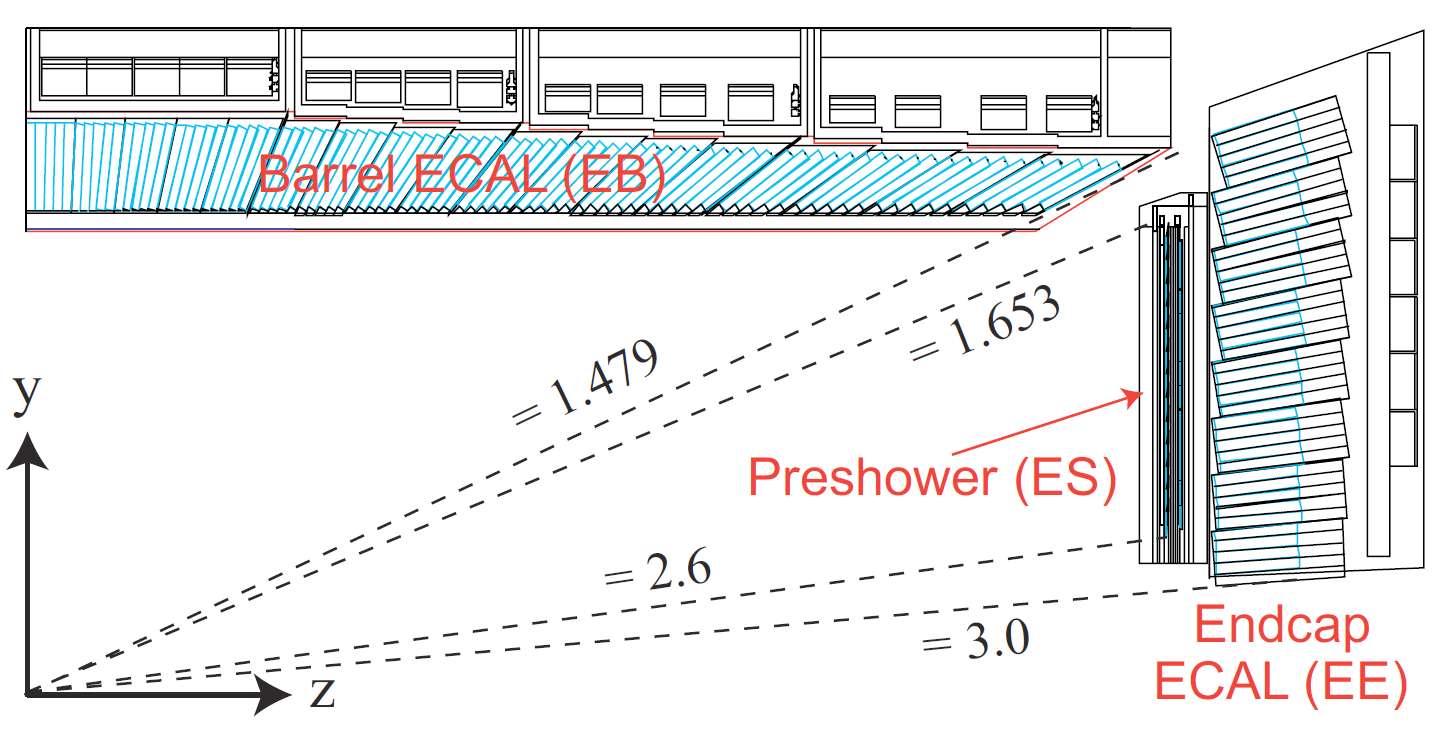
\includegraphics[width=0.89\textwidth]{figures/experiment/CMS/Figures_Experimental_Apparatus_ECALRapidity.png}
  \caption{A quarter section of the ECAL in a transverse view. Taken from~\cite{bib:CMS:TDR_2006}.}  
  \label{fig:ECAL}
\end{figure}
It can be seen, that the ECAL barrel~(EB) covers a pseudorapidity region up to $|\eta|=1.479$.
The ECAL endcaps~(EE) start at $|\eta|=1.653$ and reach up to $|\eta|=3.0$.
Before the endcaps, a preshower detector ($1.653<|\eta|<2.6$) is installed with the main task to identify neutral pions in the endcaps.
It additionally improves the position measurement of electrons and photons.

The EB and EE consist of lead tungstate (PbWO$_4$) scintillating crystals, 61200 in the barrel region and 7324 in the endcaps. 
Their advantage is the short radiation length (X$_0$=0.89\cm) and a small Moli\`ere radius (2.2\cm).
Thus, particles deposit their energy on rather short distances and a compact design is possible.
To detect the rather low light yield (30$\gamma$/\mev) of a traversing particle, silicon avalanche photodiodes (APDs) are used in the barrel region and vacuum  phototriodes (VPTs) in the endcaps.
For information on the readout electronics, the reader is referred to~\cite{bib:CMS:TDR_2006}.

The resolution of an energy measurement in the calorimeter can be expressed by 
\begin{equation}
\label{eq:CaloResolution}
\left( \frac{\sigma}{E} \right)^2 = \left( \frac{S}{\sqrt{E}} \right)^2 + \left( \frac{N}{E} \right)^2 +C^2,
\end{equation}
with $S$ referring to the stochastic term, $N$ to the noise term, and $C$ to a constant term.
For the ECAL the parameters of Eq.~\eqref{eq:CaloResolution} are measured to $S=3.63\sqrt{\text{GeV}}$, $N=0.124\gev$, and $C=0.26$~\cite{bib:CMS:TDR_2006}. 
These numbers lead to an energy resolution of around 0.4\% for an electron with $E \approx 200\gev$ and around 0.6\% for an electron with $E \approx 50\gev$.

%%%%%%%%%%%%%%%%%%%%%%%%%%%%%%%%%%%%%%%%%%%%%%%%%%%%%%%%%%%%%%%%%%%%%%%%%%%%%%%%%%%%%%%%%%%%%%%%%%%%%%%%%%%%%%%%%%%%%%%%%%%%%%%%%%%%%%%%%%%%%%%%%%%%%%%%%%%%%%%%%%%%%%%%%%%%%%%%%%%%%%%%%%%%%%%%%%%%%%%%%%%%%%%%%%%%%%%%%%%%%%%%%%
\section{The hadronic calorimeter}
The hadronic calorimeter (HCAL)~\cite{bib:CMS:TDR_2006,bib:CMS:TDR_HCAL} of the CMS detector is splitted into four different detector modules: the hadron barrel (HB), the hadron outer (HO), the hadron endcap (HE) and the hadron forward (HF) calorimeters.
A schematic sketch is depicted in Fig.~\ref{fig:HCAL}.
\begin{figure}[!ht]
  \centering
      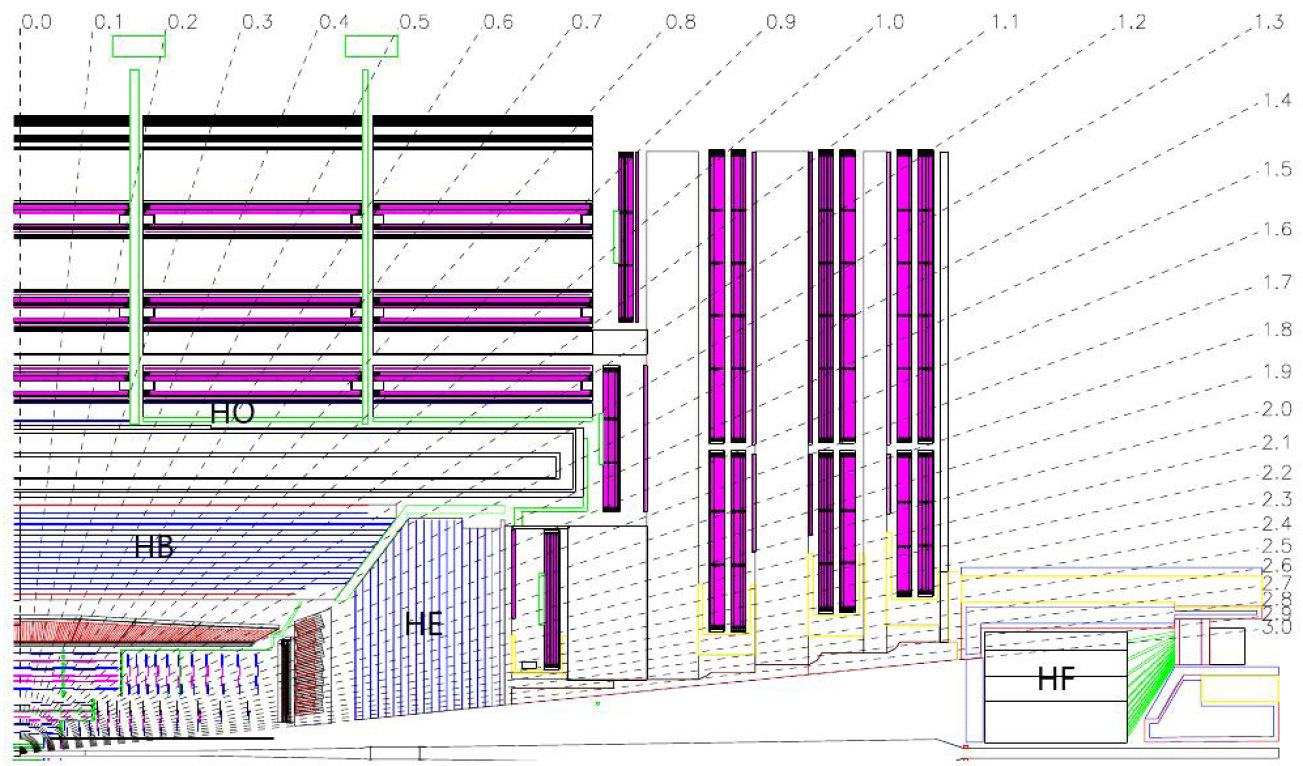
\includegraphics[width=0.79\textwidth]{figures/experiment/CMS/fig_HCALdiagram.png}
  \caption{A quarter section of the HCAL in a transverse view. Taken from~\cite{bib:CMS:HCAL_Performance_2009}.}  
  \label{fig:HCAL}
\end{figure}

The HCAL is dedicated to measuring the energy of hadrons as well as providing a good estimate of the missing energy in the event.
The latter one is achieved by the high pseudorapidity coverage ($|\eta|<5.0$) that assures the detection of most of the visible particles.

The HCAL is a so-called sampling calorimeter which consists of brass absorber material, initiating the hadronic shower, as well as active plastic scintillators.
The emitted photons are read out with wavelength-shifting (WLS) fibres which are embedded into the scintillators.
These in turn are connected to clear fibres that transfer the light to the readout system.

The hadron barrel (HB) covers the pseudorapidity range between $-1.4 < \eta < 1.4$.
It is composed of 17 layers of absorber material (15 brass and 2 steel layers) interleaved with scintillator layers.
The scintillator layers are divided into 2304 towers with a size of $\Delta \eta \times \Delta \phi = 0.087 \times 0.087$.

The hadron outer (HO) covers a pseudorapidity range up to $|\eta|=1.26$ and is divided into sectors which match the $\phi$ segmentation of the drift-tube chambers of the muon system (see Section~\ref{sec:MuonSystem}).
It is located between the solenoid and the barrel detector of the muon system.
The HO is dedicated to measuring the energy of the shower leakage of hadrons.
Its thickness corresponds to over ten interaction lengths.

The hadron endcap (HE) extends the pseudorapidity coverage of the HCAL up to $|\eta|=3.0$ and starts at $|\eta|=1.3$.
It consists of 2304 towers in total, which vary in size between $5-10\degree$ in the $\phi$ direction and $0.087-0.35$ in $\eta$ direction.

Finally, the hadron forward (HF) calorimeter extends the pseudorapidity range up to $|\eta|=5.0$, starting from $|\eta|=3.0$.
It is build out of steel plates, which contain $1\mm^2$ grooves containing quartz fibres.
The emitted light by the quartz fibres is transferred to photomultipliers.
The HF is divided into 13 towers where almost all towers have a spread of $\Delta \eta \approx 0.175$ in $\eta$ direction and $\sim 10\degree$ in $\phi$ direction.
 
%%%%%%%%%%%%%%%%%%%%%%%%%%%%%%%%%%%%%%%%%%%%%%%%%%%%%%%%%%%%%%%%%%%%%%%%%%%%%%%%%%%%%%%%%%%%%%%%%%%%%%%%%%%%%%%%%%%%%%%%%%%%%%%%%%%%%%%%%%%%%%%%%%%%%%%%%%%%%%%%%%%%%%%%%%%%%%%%%%%%%%%%%%%%%%%%%%%%%%%%%%%%%%%%%%%%%%%%%%%%%%%%%%
\section{The muon system}
\label{sec:MuonSystem}
The muon system~\cite{bib:CMS:TDR_2006,bib:CMS:TDR_MuonSystem} is the outermost detector component at CMS.
It comprises three different types of gaseous detectors, mounted into the iron return yokes: drift tube (DT) chambers in the barrel region ($|\eta|<1.2$), cathode strip chambers (CSC) in the endcap region ($1.04<|\eta|<2.4$) and resistive plate chambers (RPC) in the barrel as well as the endcap region ($|\eta|<1.6$) (see Fig.~\ref{fig:MuonSystem} for a schematic sketch of the muon system).
\begin{figure}[!b]
  \centering
      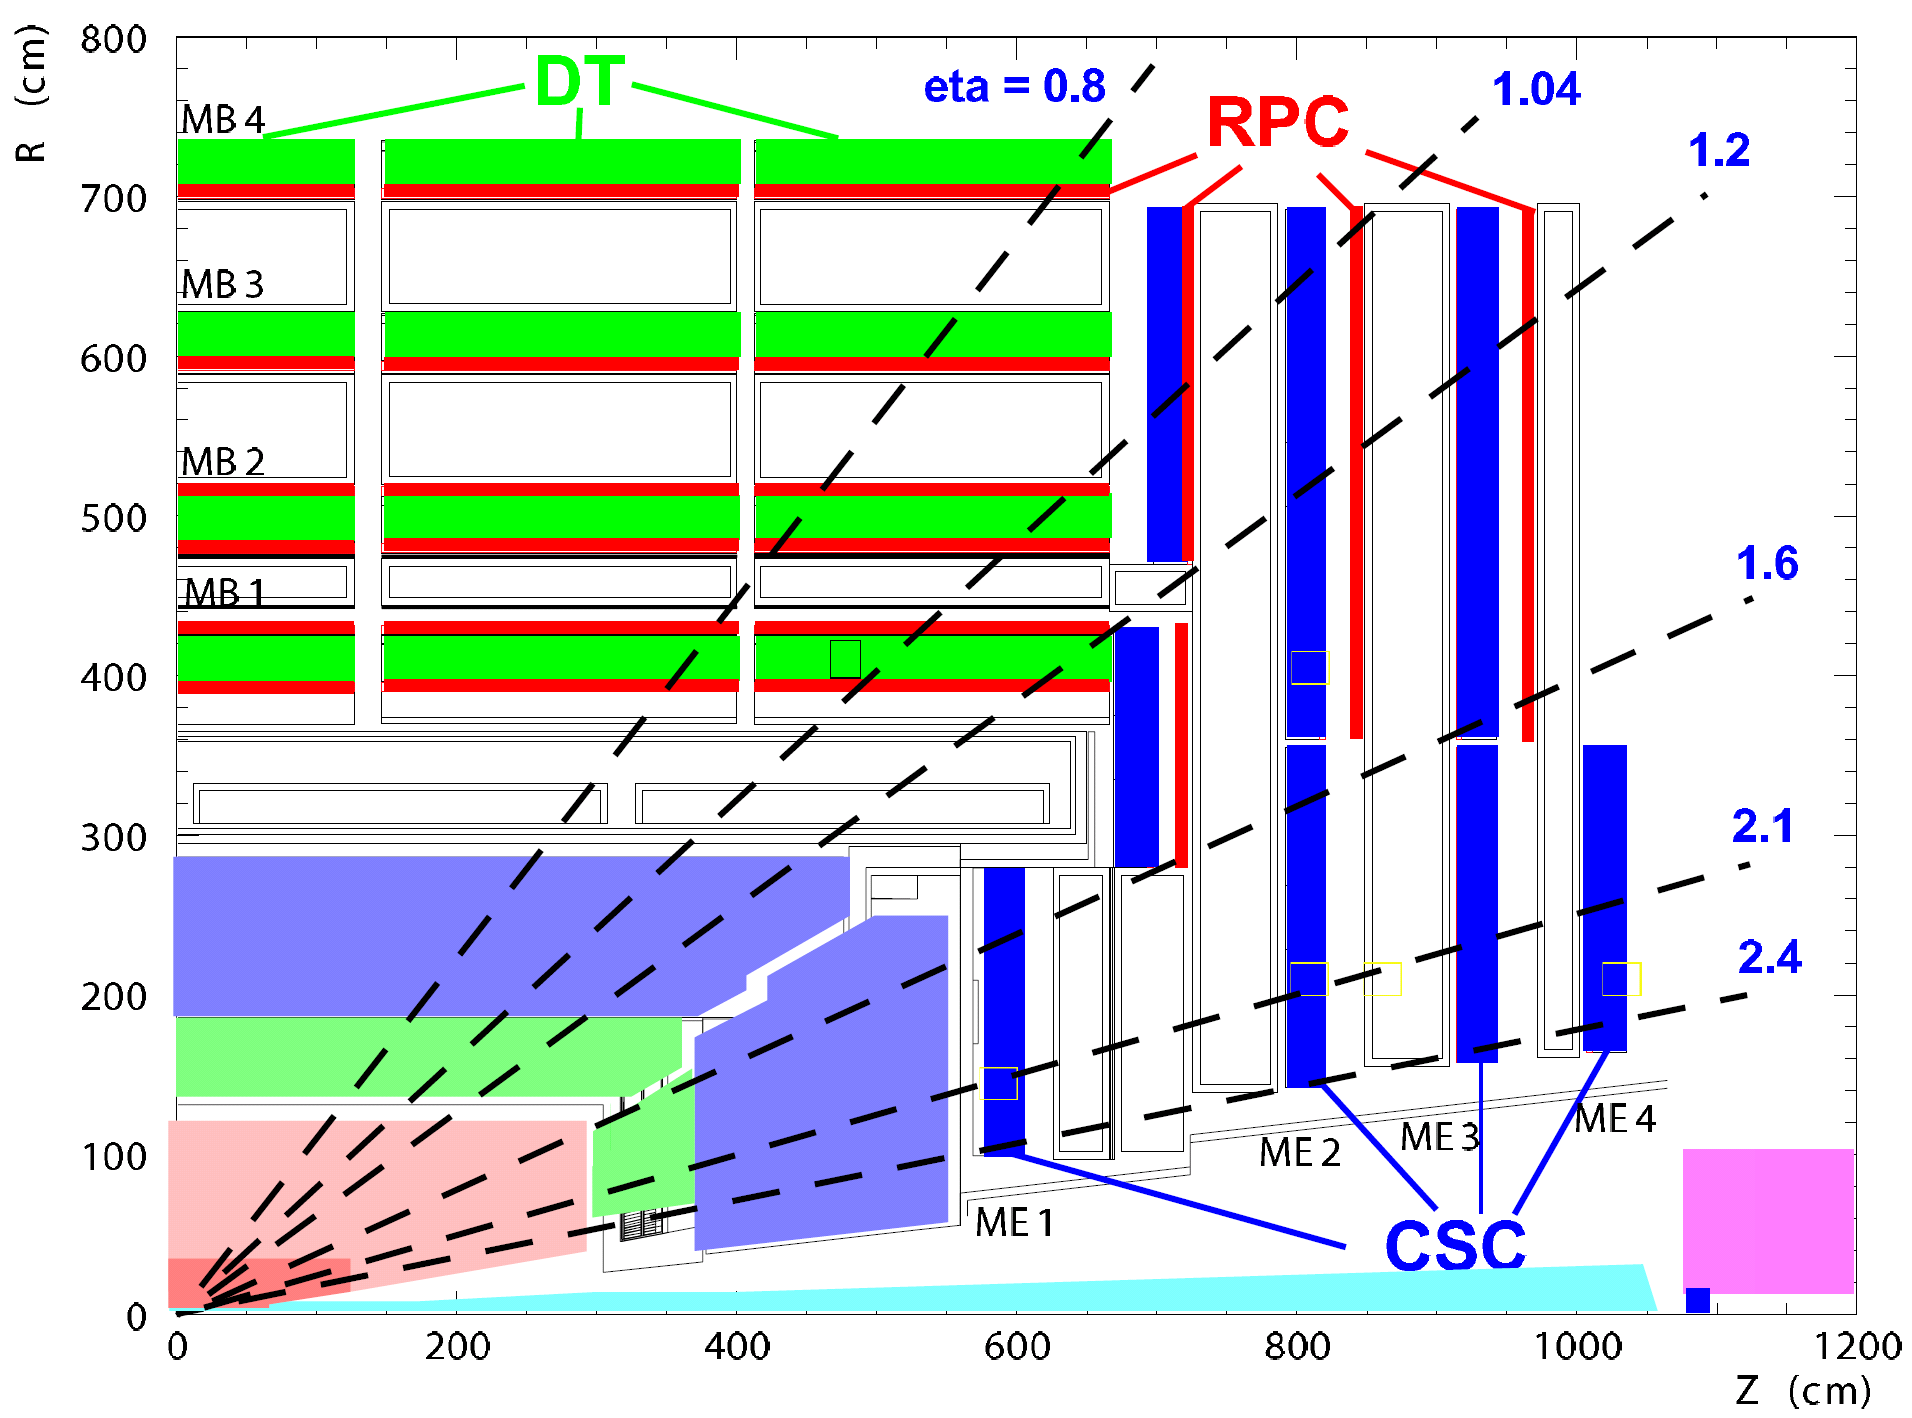
\includegraphics[width=0.69\textwidth]{figures/experiment/CMS/Figures_Experimental_Apparatus_MuonDetector.png}
  \caption{A quarter section of the CMS detector in the transverse plane with a detailed view on the muon system. Taken from~\cite{bib:CMS:TDR_2006}.}  
  \label{fig:MuonSystem}
\end{figure}
In the barrel part of the muon system, four layers (so-called stations) of drift-tube chambers are assembled inside the iron return yoke layers at radii of 4.0, 4.9, 5.9 and 7.0\m from the beam axis.
The position of a muon traversing these layers can be measured with a precision of $\approx 100\mum$ in radial direction and $\approx 1\,$mrad in $\phi$ direction. 

The four endcap disks are made up of 468 cathode strip chambers in total.
By measuring the centre-of-gravity, they achieve a spatial resolution of $\approx 100-200\mum$ and an angular resolution of $\approx 10\,$mrad in $\phi$ direction.
They are designed in order to cope with a high particle flux of about 1kHz/cm$^2$ and a non-uniform magnetic field.
As signals can be transferred very fast, they are used for the level-1 trigger system.

Finally, the resistive plate chambers cover the barrel as well as the endcap region up to a pseudorapidity of $\eta=1.6$. 
They provide a fast response with a good time resolution enabling the exact identification of the respective bunch-crossing.
It is used for the level-1 trigger system as well.
%%%%%%%%%%%%%%%%%%%%%%%%%%%%%%%%%%%%%%%%%%%%%%%%%%%%%%%%%%%%%%%%%%%%%%%%%%%%%%%%%%%%%%%%%%%%%%%%%%%%%%%%%%%%%%%%%%%%%%%%%%%%%%%%%%%%%%%%%%%%%%%%%%%%%%%%%%%%%%%%%%%%%%%%%%%%%%%%%%%%%%%%%%%%%%%%%%%%%%%%%%%%%%%%%%%%%%%%%%%%%%%%%%
\section{The trigger system}
Because of the impossibility of storing each event occurring at the CMS experiment, a multistage trigger system~\cite{bib:CMS:TDR_2006} is used to achieve a drastic reduction of recorded events by nearly six orders of magnitude.
It comprises two main parts: a so-called level-1 (L1) trigger system and a high-level trigger (HLT) system.

The L1 triggers need to provide a very fast decision (3.2\mus, where around 1\mus is allocated to the actual L1 trigger calculations) whether an event shall be recorded or not.
During this time, the recorded event data is held in buffers located close to the single detector components.
Information from the muon system and the calorimeters is used for the L1-trigger decisions.
Objects used for these decisions are so-called ``trigger primitive'' objects: photons, electrons, muons, jets above certain \et and \pt thresholds and global variables like missing transverse energy, \met. 
The design value of the number of events per second that pass this trigger stage is 100\khz.

After a time of 3.2\mus, the stored data in the buffers close to the single detector components are transferred to the front-end readout buffers in case the event passed the L1-trigger requirements.
By partial event reconstruction and the use of various trigger levels (calorimeter, muon information followed by pixel information and full event reconstruction), higher event objects can be used to check whether HLT-trigger requirements are fulfilled.
On HLT level, the decision time amounts to 50\ms and a reduction from 100\khz to 100\hz of event recording is achieved.

%%%%%%%%%%%%%%%%%%%%%%%%%%%%%%%%%%%%%%%%%%%%%%%%%%%%%%%%%%%%%%%%%%%%%%%%%%%%%%%%%%%%%%%%%%%%%%%%%%%%%%%%%%%%%%%%%%%%%%%%%%%%%%%%%%%%%%%%%%%%%%%%%%%%%%%%%%%%%%%%%%%%%%%%%%%%%%%%%%%%%%%%%%%%%%%%%%%%%%%%%%%%%%%%%%%%%%%%%%%%%%%%%%%
%%%%%%%%%%%%%%%%%%%%%%%%%%%%%%%%%%%%%%%%%%%%%%%%%%%%%%%%%%%%%%%%%%%%%%%%%%%%%%%%%%%%%%%%%%%%%%%%%%%%%%%%%%%%%%%%%%%%%%%%%%%%%%%%%%%%%%%%%%%%%%%%%%%%%%%%%%%%%%%%%%%%%%%%%%%%%%%%%%%%%%%%%%%%%%%%%%%%%%%%%%%%%%%%%%%%%%%%%%%%%%%%%%%
%%%%%%%%%%%%%%%%%%%%%%%%%%%%%%%%%%%%%%%%%%%%%%%%%%%%%%%%%%%%%%%%%%%%%%%%%%%%%%%%%%%%%%%%%%%%%%%%%%%%%%%%%%%%%%%%%%%%%%%%%%%%%%%%%%%%%%%%%%%%%%%%%%%%%%%%%%%%%%%%%%%%%%%%%%%%%%%%%%%%%%%%%%%%%%%%%%%%%%%%%%%%%%%%%%%%%%%%%%%%%%%%%%%
\FloatBarrier
\chapter{Event reconstruction and particle identification}
A crucial ingredient of data analysis at the CMS experiment, is the translation of the energy measurements in the various sub-detector components into physical objects, like muons, electrons, \etc.
For this translation, \ie particle identification, information from all detector components are used.
This is know as the particle-flow event reconstruction algorithm~\cite{CMS-PAS-PFT-09-001}.
In Fig.~\ref{fig:CMSslice}, a slice through the CMS detector is shown with the signatures of different particles indicated as coloured lines.

In the next section an introduction into this algorithm is given, followed by the definition and classification of physics objects at the CMS experiment.

\begin{figure}[!ht]
  \centering
      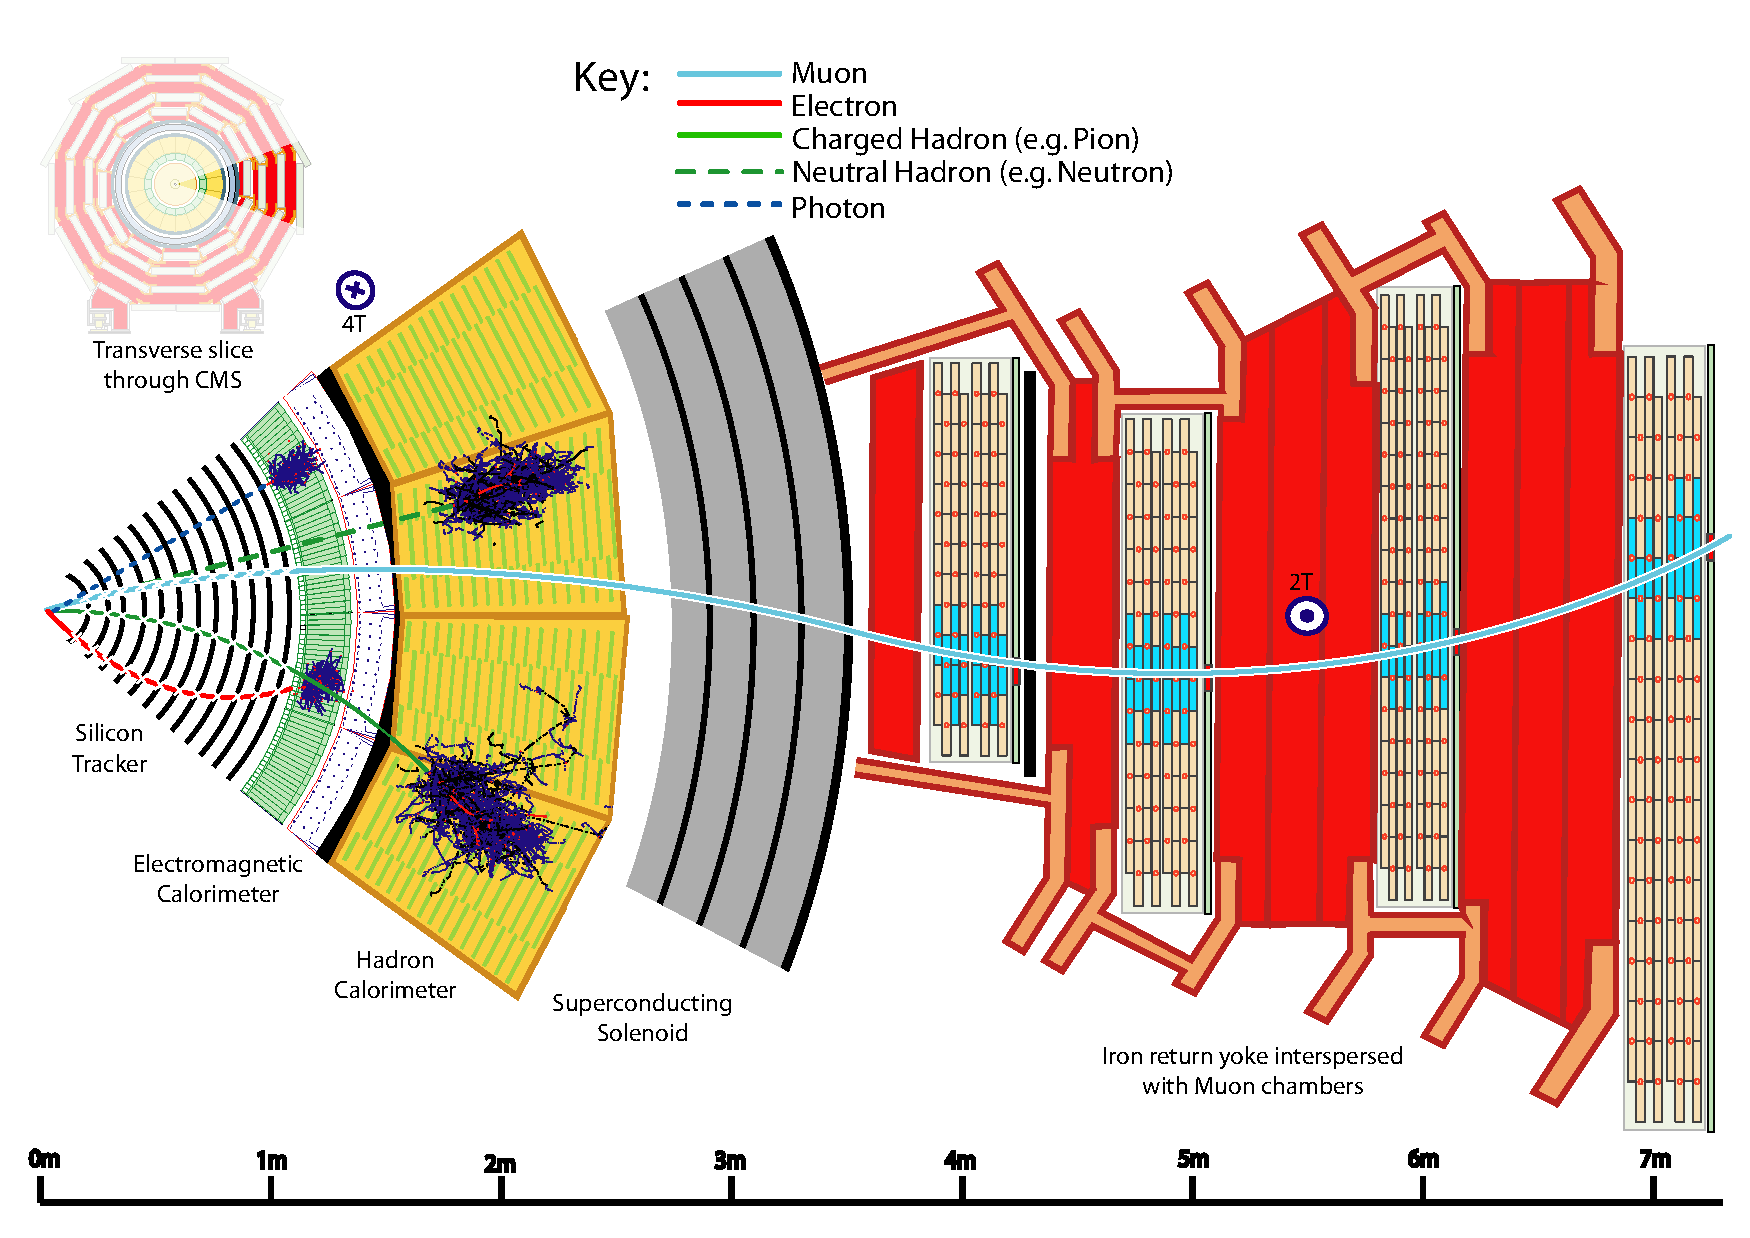
\includegraphics[width=0.99\textwidth]{figures/experiment/ObjectReconstruction/slice_white.pdf}
  \caption{A radial slice through the CMS detector with several particle signatures indicated as coloured lines.}  
  \label{fig:CMSslice}
\end{figure}

%This is done by defining what kind of energy deposits are necessary in order to classify signals during an event as a muon, \etc.
%For this classification, a certain catalogue is set up, which specifies when to classify energy signals as a certain particle.

\section{The particle-flow algorithm}
\label{sec:PFalgorithm}
The particle-flow (PF) event description~\cite{CMS-PAS-PFT-09-001} aims at optimising particle identification by the usage of all sub-detector components of the CMS detector.
There are three main building bricks used for the global event description: reconstructed charged-particle tracks, calorimeter clusters, and muon tracks.
The main requirements for these building bricks is a high reconstruction efficiency as well as a small fake rate.
Therefore, a special emphasis was put on developing a very efficient tracking algorithm (see Section~\ref{sec:ObjectReconstruction}) and a well performing calorimeter clustering algorithm~\cite{CMS-PAS-PFT-09-001}. 

The particle-flow algorithm proceeds as follows in an event (the following steps are a bit simplistic, the reader is referred to~\cite{CMS-PAS-PFT-09-001} for a detailed discussion):
\begin{enumerate}
\item For each pair of detected building bricks, a distance in the $\eta-\phi$ plane is calculated in order to quantify the quality of their link (whether the two building bricks stem from the same particle). 
\item ``Blocks'' are produced from the building bricks that are linked together (with a typical number of one, two or three building bricks contained in a block).
\item For each block the following steps are performed:
\begin{enumerate}
\item Each global muon (hits detected in the tracker as well as in the muon system) where the \pt measured in both sub-detectors is compatible with the tracker measurement only is defined as particle-flow muon and the track in both sub-detectors is removed from the event.
\item Electron reconstruction and identification follows using blocks with tracker hits and ECAL clusters. 
      For an identified particle-flow electron, the corresponding tracker hits and the ECAL clusters (including energy deposits from Bremsstrahlung photons) are removed. 
\item Tighter tracker quality criteria are applied.
\item The compatibility of the remaining ECAL and HCAL energy deposits to transverse momentum of the reconstructed tracks within a block is checked. 
      This allows for the identification of particle-flow charged hadrons with a momentum estimate using tracker and calorimeter information. 
      Only, if the energy deposits in the ECAL or HCAL are much larger than the corresponding track \pt, it gives rise to a particle-flow photon or particle-flow neutral hadron. 
      All used ECAL and HCAL clusters used for the identification as well as the reconstructed tracks are removed from the event.
\item Finally, the remaining HCAL and ECAL clusters (which are all not linked to any other building block) give rise to particle-flow photons or particle-flow neutral hadrons.
\end{enumerate}
\end{enumerate}
These identified particle-flow objects are used to identify further objects in the event, \eg the missing transverse-energy or decay products of a tau lepton.

\section{Object reconstruction}
\label{sec:ObjectReconstruction}
In this section, an overview about the required criteria for the identification of particles and other physics object is given.
\subsection*{Reconstruction of tracks}
The reconstruction of tracks aims at linking several hits in the tracking system to one reconstructed track that matches with a high probability the original trajectory of the particle.
With the track reconstruction an estimate of the particle's momentum as well as the position can be achieved.
The challenge arise due to the high combinatorial complexity because of the large number of hits detected in each event, especially in the layers close to the interaction vertex.
In the following an overview about the tracking algorithm used at CMS is given.
The reader is referred to~\cite{bib:CMS:tracking_8TeV} for a thorough description of the reconstruction of tracks at CMS.

The developed tracking software used at CMS is usually referred to as the Combinatorial Track Finder (CTF).
It grounds on the so-called combinatorial Kalman filter~\cite{bib:TrackAlgorithm_1989,bib:TrackAlgorithm_1990,bib:TrackAlgorithm_1997}, which is mathematically equivalent to a global least square minimisation for linear models with Gaussian noise.

The basic idea of the tracking algorithm at CMS is to not apply the combinatorial Kalman filter on all hits in one step but to reduce the level of complexity by an iterative procedure (called iterative tracking).
A reduction of complexity can be achieved by reconstructing tracks in the first step that are easy to identify because of \eg a high \pt. 
These tracks are removed afterwards and the remaining tracker hits are subject to further reconstruction iterations.
%In the following, the various iteration steps are described.
%These were in place in the year 2011.
%Adjustment in the algorithm were applied due to higher pileup conditions in the year 2012.
%However, the principle structure of the tracking algorithm remained.
The following iterations are performed:
\begin{itemize}
\item Iteration 0: Tracks near to the $pp$ interaction point that have three pixel hits and a $\pt>0.8\gev$ are reconstructed.
\item Iteration 1: Tracks with only two pixel hits and $\pt>0.8\gev$ are recovered.
\item Iteration 2: Low \pt tracks from the $pp$ interaction point are reconstructed.
\item Iteration 3-5: Reconstruction of tracks that are not originating from the primary vertex and recovering of tracks not found by previous iterations
\end{itemize}
Within these iterations, the reconstruction is subdivided into four different steps:
\begin{itemize}
\item Seed generation: Only 2-3 hits are used to define track candidates.
\item Extrapolation: Based on expected flight path, additional hits are assigned to the candidate track (use of Kalman filter)
\item Parameter estimates: With the usage of the Kalman filter and a smoother the trajectory parameters are determined
\item Setting of quality flags: Quality flags are assigned to all tracks and tracks that fail certain quality criteria are discarded.
\end{itemize}
The configuration of the first and the fourth step differ across the different iterations.  

\subsection*{Reconstruction of jets} 
The reconstruction of jets is done by a anti-kt method at CMS.
\begin{itemize}
\item Clustering methods: anti kt method
\item jet energy corrections
\end{itemize}

\subsection{Reconstruction of muons}
There are three different muon definitions at CMS~\cite{bib:CMS:muon_recoEff}: global muons (correspond to particle-flow muons), tracker muons, and standalone muons.
They have all in common that they require energy deposits in the muon system.
The reconstruction of each of the three muon types is explained in the following.
\begin{description}
\item \textbf{Standalone muons:} For the reconstruction of standalone muons, all reconstructed segments in the muon system are utilised. Similar to the track reconstruction in the tracking system, Kalman filter techniques~\cite{bib:KalmanFilter_1987} are exploited to reconstruct muon trajectories in the muon chambers.
A compatibility to the interaction point is imposed to reconstruct only muons produced at the LHC (no cosmic muons).
Further details about the reconstruction of standalone muons can be found in~\cite{bib:StandaloneMuonReconstruction,bib:CMS:TDR_2006} 
\item \textbf{Tracker muons:} To reconstruct so-called tracker muons, all tracker tracks with a $\pt>0.5\gev$ and $p>2.5\gev$ are extrapolated to the muon system. If at least one muon segment is matched to a reconstructed track within certain quality criteria, the trajectory is considered as a tracker muon (see~\cite{bib:CMS:muon_recoEff} for more detailed information).
\item \textbf{Global muons:} For the reconstruction of global muons an outside-in approach is utilised. For each reconstructed standalone muon, the compatibility to the reconstructed tracks in the tracking system is checked. If compatible, a global muon track is reconstructed using Kalman filter techniques. For high-\pt muons, the momentum resolution can be increased compared to the momentum estimated using tracker information only~\cite{bib:CMS:muon_recoEff}.
\end{description}

\subsection{Reconstruction of electrons}
The reconstruction of electrons at the CMS experiment is based on a mixture of the particle-flow algorithm explained in Section~\ref{sec:PFalgorithm} and a standalone approach~\cite{bib:StandaloneElectronReconstruction}.
Thus, it is a very complex procedure and a complete description would go beyond the scope of this thesis.
Therefore, only the rough idea of the electron reconstruction shall be reviewed here.
The reader is referred to~\cite{bib:CMS:elec_recoEff} for a complete description of the reconstruction procedure.

The difficulty of the electron reconstruction lies in the possibly large energy losses due to bremsstrahlung.
This can change the direction of the electron significantly and lead to a reduced efficiency of the standard track reconstruction used for tracker tracks.
Therefore, an optimised track reconstruction for electrons is performed in order to account for direction changes due to the radiation of photons.
Because the dedicated electron track reconstruction can be very time consuming, a seeding of tracker hits rely already on ECAL information to reduce the number of candidate tracks.


\subsection*{Reconstruction of taus}
\subsection*{Reconstruction of missing transverse energy}
\section*{Event cleaning}




%%%%%%%%%%%%%%%%%%%%%%%%%%%%%%%%%%%%%%%%%%%%%%%%%%%%%%%%%%%%%%%%%%%%%%%%%%%%%%%%%%%%%%%%%%%%%%%%%%%%%%%%%%%%%%%%%%%%%%%%%%%%%%%%%%%%%%%%%%%%%%%%%%%%%%%%%%%%%%%%%%%%%%%%%%%%%%%%%%%%%%%%%%%%%%%%%%%%%%%%%%%%%%%%%%%%%%%%%%%%%%%%%%%
%%%%%%%%%%%%%%%%%%%%%%%%%%%%%%%%%%%%%%%%%%%%%%%%%%%%%%%%%%%%%%%%%%%%%%%%%%%%%%%%%%%%%%%%%%%%%%%%%%%%%%%%%%%%%%%%%%%%%%%%%%%%%%%%%%%%%%%%%%%%%%%%%%%%%%%%%%%%%%%%%%%%%%%%%%%%%%%%%%%%%%%%%%%%%%%%%%%%%%%%%%%%%%%%%%%%%%%%%%%%%%%%%%%
%%%%%%%%%%%%%%%%%%%%%%%%%%%%%%%%%%%%%%%%%%%%%%%%%%%%%%%%%%%%%%%%%%%%%%%%%%%%%%%%%%%%%%%%%%%%%%%%%%%%%%%%%%%%%%%%%%%%%%%%%%%%%%%%%%%%%%%%%%%%%%%%%%%%%%%%%%%%%%%%%%%%%%%%%%%%%%%%%%%%%%%%%%%%%%%%%%%%%%%%%%%%%%%%%%%%%%%%%%%%%%%%%%%
\FloatBarrier
\chapter{Event simulation}

Needed:
\begin{itemize}
\item Some information on simulation
\item PDF !
\end{itemize}

3-4 pages


%  \part{A search for highly ionising, short tracks at the CMS detector}  \label{part:analysis}
%  %%%%%%%%%%%%%%%%%%%%%%%%%%%%%%%%%%%%%%%%%%%%%%%%%%%%%%%%%%%%%%%%%%%%%%%%%%%%%%%%%%%%%%%%%%%%%%%%%%%%%%%%%%%%%%%%%%%%%%%%%%%%%%%%%%%%%%%%%%%%%%%%%%%%%%%%%%%%%%%%%%%%%%%%%%%%%%%%%%%%
%%%%%%%%%%%%%%%%%%%%%%%%%%%%%%%%%%%%%%%%%%%%%%%%%%%%%%%%%%%%%%%%%%%%%%%%%%%%%%%%%%%%%%%%%%%%%%%%%%%%%%%%%%%%%%%%%%%%%%%%%%%%%%%%%%%%%%%%%%%%%%%%%%%%%%%%%%%%%%%%%%%%%%%%%%%%%%%%%%%%
\FloatBarrier
\chapter{Motivation}
\label{sec:Motivation}
R-parity conserving supersymmetric models are able to offer solutions to many unexplained phenomena in astrophysics and can solve many of the shortcomings of the Standard Model of particle physics (see Section~\ref{ch:Supersymmetry}).
While supersymmetric models, especially the Minimal Supersymmetric Standard Model (MSSM) (Section~\ref{sec:MSSM}), have been studied at previous particle colliders including Tevatron and LEP~\cite{bib:Tevatron:SUSY_results,bib:LEP:SUSY_results}, the LHC with its high centre-of-mass energy offers a unique opportunity to investigate SUSY models with high particle masses that were not accessible in previous experiments.

Therefore, a variety of searches were hunting for SUSY during Run\,I of the LHC from 2010 to 2012.
Proton-proton collision data from the CMS and ATLAS experiments were analysed with a strong focus on the search for SUSY in production channels via the strong interaction (\eg~\cite{bib:CMS:RA2_8TeV,bib:CMS:MT2_8TeV,bib:ATLAS:JetPlusMET_8TeV}).
As a consequence, wide, previously unexplored regions of the MSSM parameter space are already excluded.
However, due to the unknown mechanism of supersymmetry breaking, the most general parametrisation of the MSSM introduces over 100 new parameters and thus opens up an incredibly large phenomenological space. 
Therefore, SUSY models can lead to a plethora of possible signatures at particle colliders, many of which could not - or not fully - be explored. \\

%Among more ``exotic'' SUSY scenarios are models with compressed spectra, where two or more particles are nearly mass-degenerate.
%Especially scenarios with a nearly mass-degenerate lightest chargino (\chipm) and lightest neutralino (\chiO) are very interesting from a theoretical and cosmological perspective as they can help to explain the sources of the relic den%sity~\cite{bib:Moroi:DarkMatter_1999,bib:Hisano:DarkMatter_2005,bib:Ibe:DarkMatter_2015}.
%While it is not possible to explain the full relic density with thermally produced neutralinos for m$_{\chiO}\lesssim 2.9\tev$~\cite{bib:Moroi:DarkMatter_2013}, neutralinos can still be the dominant part if they are non-thermally produ%ced via the decay of a long-lived particle such as a wino-like chargino.
%The enhanced annihilation cross section (called Sommerfeld enhancement) into $WW$- , $ZZ$- or $ff$-pairs for a wino-like dark matter candidate leads to an underprediction of the relic density if the neutralino and chargino masses are t%oo small~\cite{bib:Hisano:DarkMatter_2003}.
%This underprediction can be cured, however, if there is an additional non-thermal production of dark matter that is caused by the decay of a long-lived chargino.


%Among more ``exotic'' SUSY scenarios are models with compressed spectra, where two or more particles are nearly mass-degenerate.
%Especially scenarios with a wino-like 
%Especially scenarios with a nearly mass-degenerate lightest chargino (\chipm) and lightest neutralino (\chiO) are very interesting from a theoretical and cosmological perspective as they can help to explain the sources of the relic den%sity~\cite{bib:Moroi:DarkMatter_1999,bib:Hisano:DarkMatter_2005,bib:Ibe:DarkMatter_2015}.
%While it is not possible to explain the full relic density with thermally produced neutralinos for m$_{\chiO}\lesssim 2.9\tev$~\cite{bib:Moroi:DarkMatter_2013}, neutralinos can still be the dominant part if they are non-thermally produ%ced via the decay of a long-lived particle such as a wino-like chargino.
%The enhanced annihilation cross section (called Sommerfeld enhancement) into $WW$- , $ZZ$- or $ff$-pairs for a wino-like dark matter candidate leads to an underprediction of the relic density if the neutralino and chargino masses are t%oo small~\cite{bib:Hisano:DarkMatter_2003}.
%This underprediction can be cured, however, if there is an additional non-thermal production of dark matter that is caused by the decay of a long-lived chargino.

A very interesting signature occurs when particles live long enough to travel through a part or the whole detector before decaying.
This is possible for SUSY models with compressed spectra, in which a particle can be long-lived because of phase-space suppression.
In the MSSM, such a mass-degeneracy naturally occurs if the wino mass parameter ($M_2$) is smaller than the bino ($M_1$) and higgsino ($\mu$) mass parameters.
In this case, the lightest chargino (\chipm) and the lightest neutralino (\chiO) are both wino-like and their mass gap is fully determined by higher order corrections (see Section~\ref{ch:Longlived_Particles}). 
Therefore, they are almost mass-degenerate and the chargino is long-lived.

Such scenarios can be very interesting from a cosmological perspective as the wino-like lightest supersymmetric particle, the neutralino \chiO, can serve as a plausible Dark Matter candidate~\cite{bib:Ibe:DarkMatter_2015,bib:Hisano:DarkMatter_2005}.
While it is not possible to explain the full relic density with thermally produced wino-like neutralinos for m$_{\chiO}\lesssim 3\tev$~\cite{bib:IndirectSearches_Cohen_2013}, neutralinos can still be the dominant part if they are non-thermally produced via the decay of an almost decoupled particle~\cite{bib:Moroi:DarkMatter_1999,bib:Moroi:DarkMatter_2013}.
%Even if the wino-like neutralino is not able to explain the full relic density, it remains theoretically motivated as long as it does not leave excessive relics.

Additionally, explorations of the MSSM parameter space reveal that many models that are consistent with current observations and theoretical constraints and that offer a neutralino as Dark Matter candidate include a metastable chargino with a mass gap of the order of~$\sim160\mev$ with respect to the neutralino~\cite{bib:pMSSMScan_2013}.\\

%Additionally, these scenarios are well motivated by Supersymmetric models with anomaly-mediated SUSY breaking (AMSB)~\cite{bib:Theory_AMSB_1998,bib:Theory_AMSB_1999}, where the LSP is almost always the wino-like lightest neutralino and the mass gap between the neutralino and chargino is typically between 140\mev and 200\mev~\cite{bib:Theory_MassGap_2014}.\\
%The enhanced annihilation cross section (called Sommerfeld enhancement) into $WW$- , $ZZ$- or $ff$-pairs for a wino-like dark matter candidate leads to an underprediction of the relic density if the neutralino mass is too small~\cite{bib:Hisano:DarkMatter_2003}.
%This underprediction can be cured, however, if there is an additional non-thermal production of dark matter as explained before.

SUSY scenarios with nearly mass-degenerate particles have two distinctive phenomenological properties that require a very different search strategy compared to general SUSY searches. 
First, because of the mass-degeneracy, the remaining decay product (\eg a pion) is very soft in \pt, making it hard to detect.
Since the other decay product, the neutralino, is only weakly interacting, it is very difficult to identify charginos via their decay products. 
% makes the detection of the chargino by the decay products a challenging task. 
%First, if the chargino and the neutralino are almost mass-degenerate, the remaining decay product (\eg a pion) is very soft in \pt, making it hard to detect.
Second, as the chargino is long-lived, it may traverse several detector layers before decaying.
Thus, there is the possibility of reconstructing the chargino itself, \eg as a reconstructed track in the tracker system.\\
%However, how the chargino is reconstructed is highly dependent on its concrete lifetime.
%However, depending on the concrete lifetime of the chargino, the reconstruction of the chargino this reconstruction can require very different tools compared to the reconstruction of Standard Model particles.

%Even though supersymmetric models with nearly mass-degenerate \chipm and \chiO lead to exotic signatures with long-lived charginos and soft decay products, current CMS searches are already sensitive over a very broad range of lifetimes.

Despite the exotic signatures of supersymmetric models with nearly mass-degenerate \chipm and \chiO, current CMS searches are already sensitive to a very broad range of lifetimes.
The exclusion power of existing SUSY searches can be assessed by interpreting their results in terms of the fraction of excluded parameter points in the phenomenological MSSM (see Section~\ref{subsec:pMSSM} for an introduction to the pMSSM). 
The results of such a study which has been performed in \cite{bib:CMS:DT_8TeV} are shown in Figure~\ref{fig:pMSSMplot}. 
\begin{figure}[!t]
\vspace{20pt}
  \centering 
  \begin{tabular}{c}
    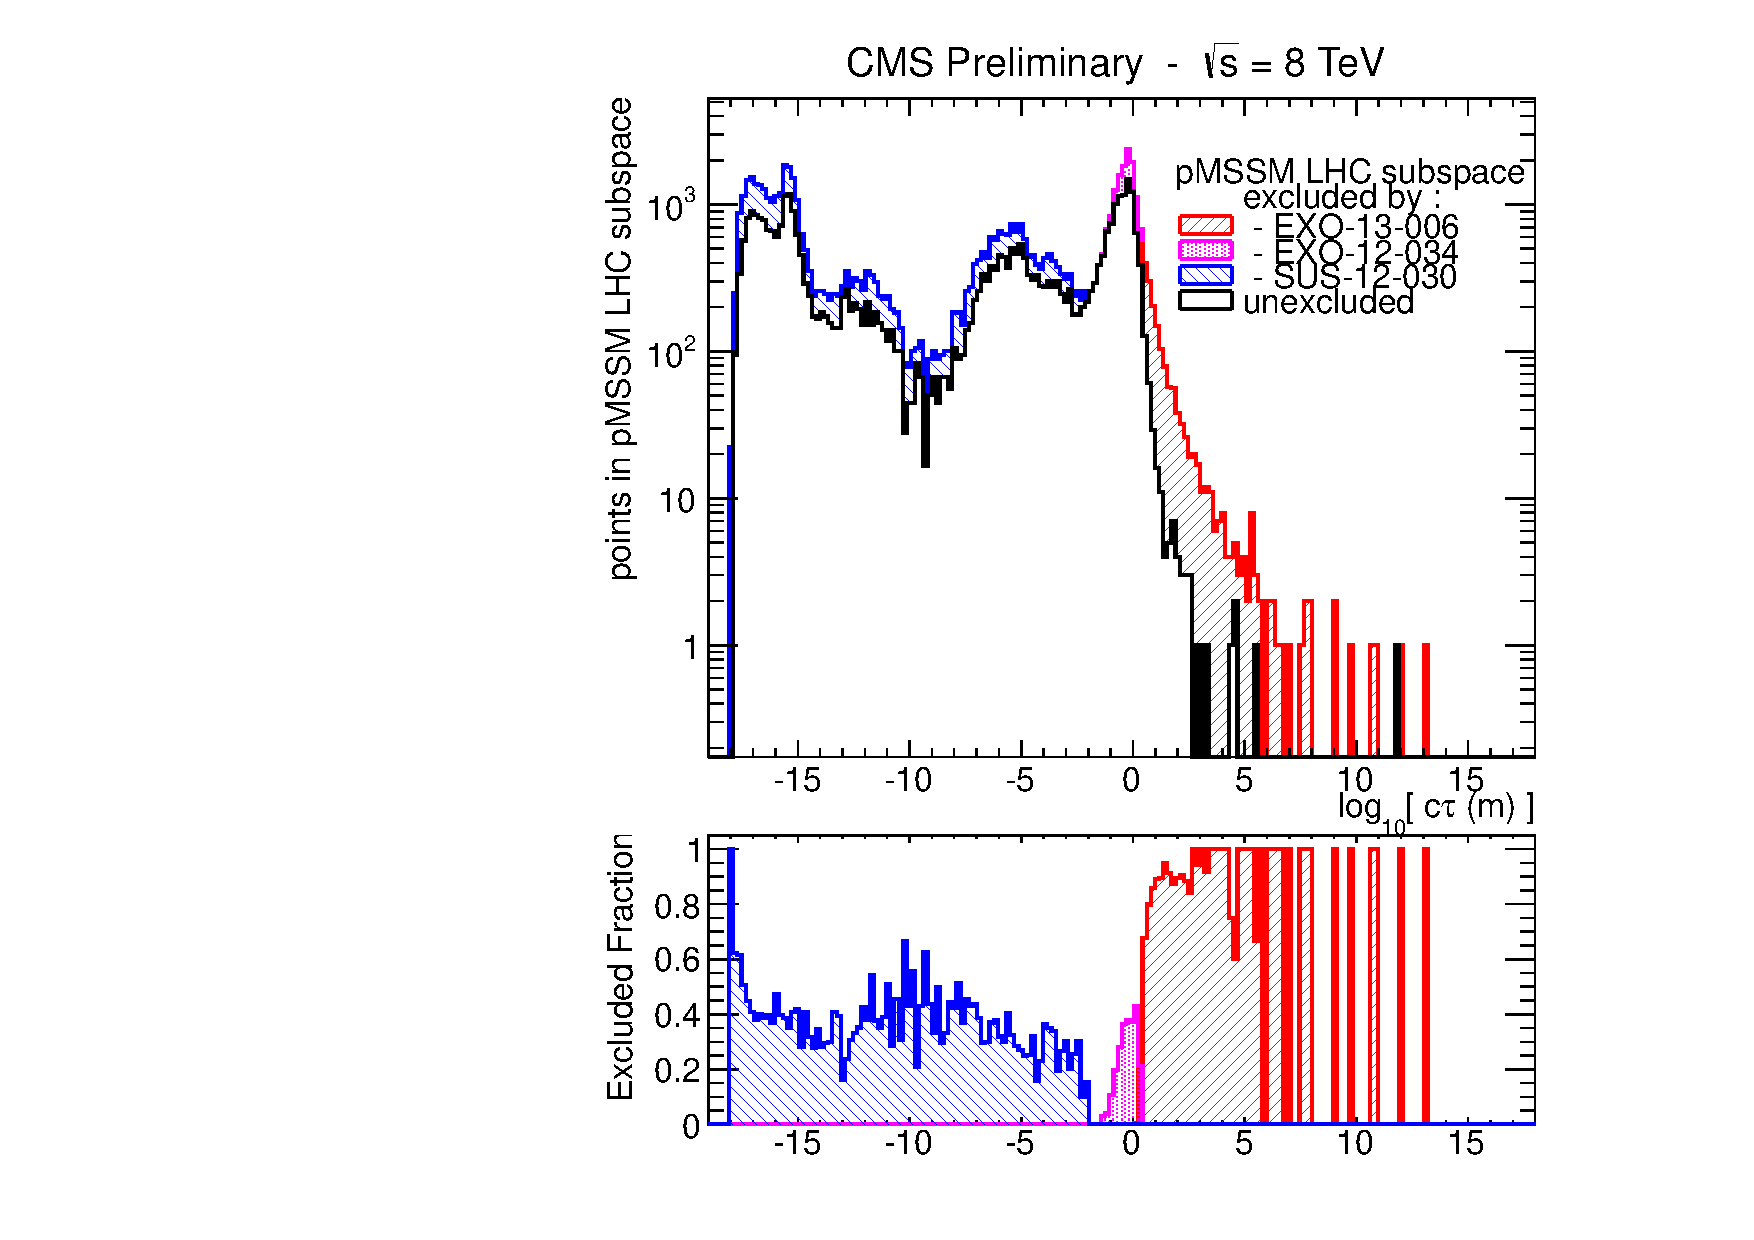
\includegraphics[width=0.75\textwidth]{figures/analysis/pMSSM_vs_ctau.pdf}
  \end{tabular}
  \caption{The number of excluded pMSSM points at 95\% C.L. (upper part) and the fraction of excluded pMSSM points (bottom part) vs. the chargino lifetime for different CMS searches.
           Red area: the search for long-lived charged particles \cite{bib:CMS:HSCP_8TeV},
           Purple area: the search for disappearing tracks  \cite{bib:CMS:DT_8TeV},
           Blue area: a collection of various general SUSY searches \cite{bib:CMS:pMSSMinterpretation_7TeV_PAS}
           The black line indicates the unexcluded pMSSM parameter points.
           The sampling of the parameter space points was done according to a prior probability density function which takes pre-LHC data and results from indirect SUSY searches into account (see \cite{bib:CMS:HSCPReinterpreation_PAS} for further details).
           Taken from: \cite{bib:pMSSMplot_source_from_DT}.}
  \label{fig:pMSSMplot}
\vspace{20pt}
\end{figure}
It can be seen that general SUSY searches (blue area) are sensitive to shorter chargino lifetimes ($c\tau \lesssim 1\cm$).\footnote{Since the pMSSM interpretation relied on the use of fast simulation techniques which are not capable of simulating charginos with lifetimes $\ctau>1\cm$, the general SUSY searches were never interpreted in the context of SUSY models with longer chargino lifetimes.} 
%Due to technical reasons\footnote{The pMSSM interpretation relied on the use of fast simulation techniques which are not capable of simulating charginos with lifetimes $\ctau>1\cm$.}, the general SUSY searches were never interpreted in the context of SUSY models with longer chargino lifetimes. 
Two existing searches, the search for long-lived charged particles~\cite{bib:CMS:HSCP_8TeV} and the search for disappearing tracks~\cite{bib:CMS:DT_8TeV} focus on long and intermediate chargino lifetimes, respectively. 
These two searches (purple and red areas) are sensitive to chargino lifetimes of $\ctau \gtrsim 10\cm$.
Taken together, the existing searches exclude a large fraction of pMSSM points at different chargino lifetimes. 
However, there is a gap between the general SUSY searches and the search for disappearing tracks that is not accessible by any of the existing searches.\\

The here presented analysis aims at targeting this gap by optimising the search strategy for charginos with intermediate lifetimes of $1\cm \lesssim c\tau \lesssim 30\cm$. 
The targeted optimisation strategy is a combination of the strategies used in the search for long-lived charged particles~\cite{bib:CMS:HSCP_8TeV} and the search for disappearing tracks~\cite{bib:CMS:DT_8TeV}.
While in~\cite{bib:CMS:HSCP_8TeV}, the high ionisation losses of hypothetical new massive particles is exploited, it does not take into account whether its reconstructed track is disappearing.
In~\cite{bib:CMS:DT_8TeV}, the disappearance of the track is utilised but it does not incorporate the large ionisation losses into the search.
Additionally, neither of the search does take into account the possibly very short tracks of early decaying charginos.\\

Thus, the here presented search is the first analysis at CMS combining the two signature properties that are highly distinctive for charginos with intermediate lifetimes: 
first, the characteristically high ionisation losses of heavy charginos;
second, short reconstructed tracks due to chargino decays early in the detector. \\

The associated challenges and the general search strategy of this analysis will be presented in the next section.

%%%%%%%%%%%%%%%%%%%%%%%%%%%%%%%%%%%%%%%%%%%%%%%%%%%%%%%%%%%%%%%%%%%%%%%%%%%%%%%%%%%%%%%%%%%%%%%%%%%%%%%%%%%%%%%%%%%%%%%%%%%%%%%%%%%%%%%%%%%%%%%%%%%%%%%%%%%%%%%%%%%%%%%%%%%%%%%%%%%%
%%%%%%%%%%%%%%%%%%%%%%%%%%%%%%%%%%%%%%%%%%%%%%%%%%%%%%%%%%%%%%%%%%%%%%%%%%%%%%%%%%%%%%%%%%%%%%%%%%%%%%%%%%%%%%%%%%%%%%%%%%%%%%%%%%%%%%%%%%%%%%%%%%%%%%%%%%%%%%%%%%%%%%%%%%%%%%%%%%%%

%  %%%%%%%%%%%%%%%%%%%%%%%%%%%%%%%%%%%%%%%%%%%%%%%%%%%%%%%%%%%%%%%%%%%%%%%%%%%%%%%%%%%%%%%%%%%%%%%%%%%%%%%%%%%%%%%%%%%%%%%%%%%%%%%%%%%%%%%%%%%%%%%%%%%%%%%%%%%%%%%%%%%%%%%%%%%%%%%%%%%%
%%%%%%%%%%%%%%%%%%%%%%%%%%%%%%%%%%%%%%%%%%%%%%%%%%%%%%%%%%%%%%%%%%%%%%%%%%%%%%%%%%%%%%%%%%%%%%%%%%%%%%%%%%%%%%%%%%%%%%%%%%%%%%%%%%%%%%%%%%%%%%%%%%%%%%%%%%%%%%%%%%%%%%%%%%%%%%%%%%%%
%%%%%%%%%%%%%%%%%%%%%%%%%%%%%%%%%%%%%%%%%%%%%%%%%%%%%%%%%%%%%%%%%%%%%%%%%%%%%%%%%%%%%%%%%%%%%%%%%%%%%%%%%%%%%%%%%%%%%%%%%%%%%%%%%%%%%%%%%%%%%%%%%%%%%%%%%%%%%%%%%%%%%%%%%%%%%%%%%%%%
\FloatBarrier
\chapter{General search strategy}
\label{sec:GeneralSearchStrategy}

At the LHC, there are several possible chargino production channels. 
Chargino pairs can be produced through a photon or a $Z$-boson exchange. 
The chargino then decays via a virtual $W$-boson to the lightest neutralino and a fermion pair (\eg a pion). 
This process is illustrated in the Feynman diagram in Fig.~\ref{fig:FeynmanDiagram}.
Other possible chargino pair production channels include the exchange of a supersymmetric Higgs boson or a t-channel squark exchange (Fig.~\ref{fig:FeynmanDiagramProductionCharginoPair}).

Apart from pair production, charginos can be produced via the chargino-neutralino channel. 
On tree-level, there exist two production mechanisms: the s-channel $W$-boson exchange and the t-channel squark exchange (Fig.~\ref{fig:FeynmanDiagramProductionCharginoNeutralino}).
\begin{figure}[!b]
  \centering 
  \begin{tabular}{c}
    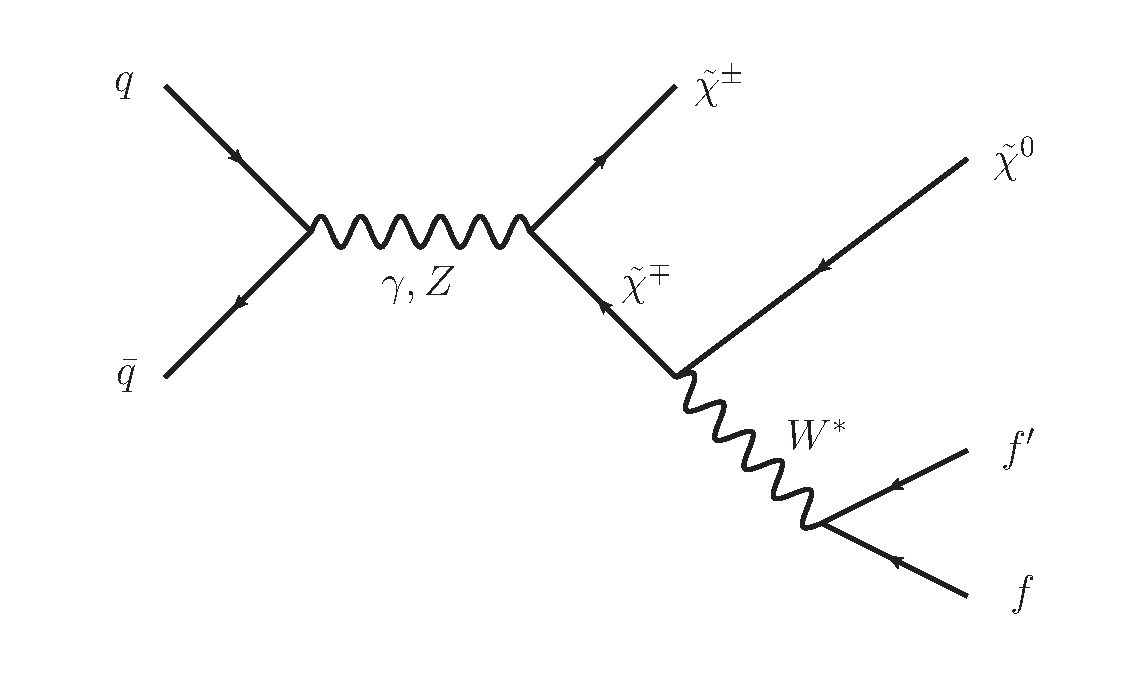
\includegraphics[width=0.75\textwidth]{figures/analysis/ChiChi_ProductionAndDecay.pdf}
  \end{tabular}
  \caption{Feynman diagram of chargino pair production via gamma or $Z$-boson exchange and the subsequent decay via a virtual $W$-boson.}
  \label{fig:FeynmanDiagram}
\end{figure}

\begin{figure}[!h]
  \centering 
  \begin{tabular}{c}
    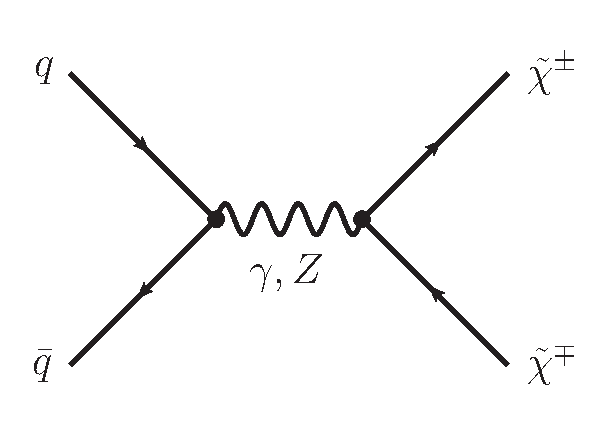
\includegraphics[width=0.33\textwidth]{figures/analysis/ChiChi_GammaZ.pdf}
    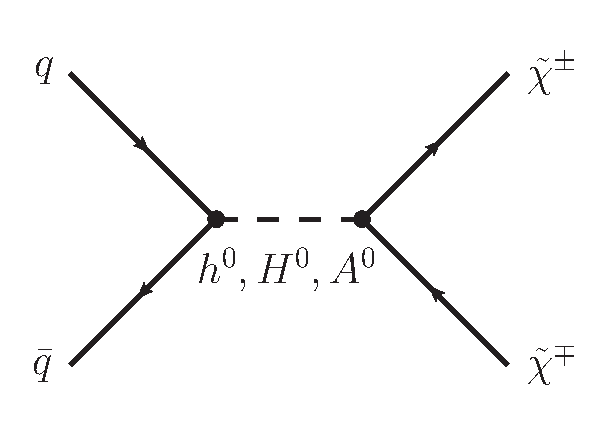
\includegraphics[width=0.33\textwidth]{figures/analysis/ChiChi_Scalar.pdf}
    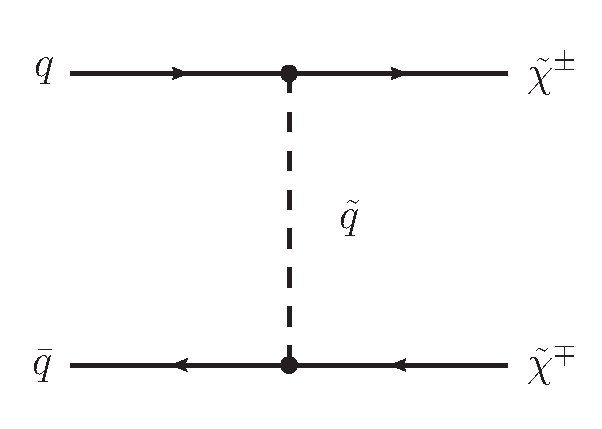
\includegraphics[width=0.33\textwidth]{figures/analysis/ChiChi_Squark.pdf}
  \end{tabular}
  \caption{Main tree-level diagrams for chargino pair production.}
  \label{fig:FeynmanDiagramProductionCharginoPair}
\end{figure}

\begin{figure}[!h]
  \centering 
  \begin{tabular}{c}
    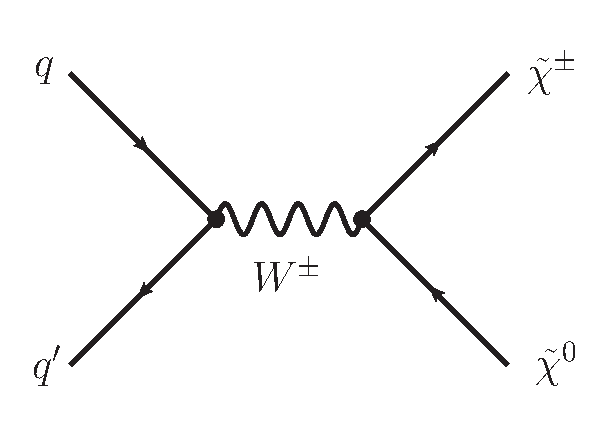
\includegraphics[width=0.33\textwidth]{figures/analysis/ChiChi0_WBoson.pdf}
    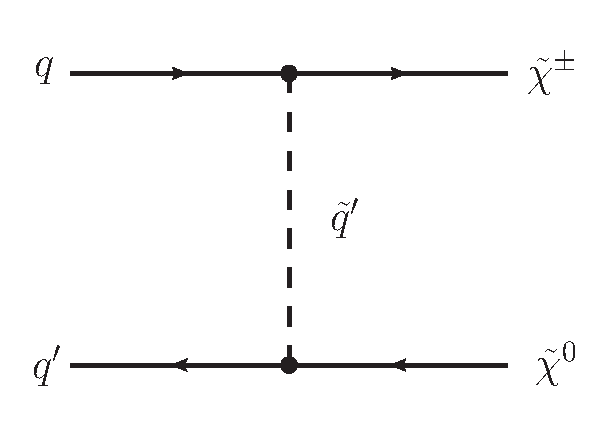
\includegraphics[width=0.33\textwidth]{figures/analysis/ChiChi0_Squark.pdf}
  \end{tabular}
  \caption{Main tree-level diagrams for chargino neutralino production.}
  \label{fig:FeynmanDiagramProductionCharginoNeutralino}
\end{figure}
Alternatively, charginos can be produced via strong production modes, \ie in cascade decays of new heavy particles, such as gluinos or squarks.
In the here presented search, the focus is, however, put on the electroweak production channels: chargino pair and chargino-neutralino production.\\


When searching for supersymmetric models with long-lived \chipm, the strategy is of course highly dependent on the actual lifetime of the chargino. 
For long lifetimes, the chargino can reach the muon chambers and can be reconstructed as a muon even despite a longer time-of-flight~\cite{bib:CMS:HSCP_7TeV}. 
For lower lifetimes, the chargino can already decay inside the detector (\eg the tracker), and hence can not be reconstructed as a muon but leads to an isolated, potentially disappearing track in the tracker. 
The detector signatures of these two scenarios are visualised in Fig.~\ref{fig:CharginoPaiEventDisplay}, where simulated chargino-chargino events are shown in a cross-sectional view of the CMS detector.
\begin{figure}[!t]
  \centering 
  \begin{tabular}{c}
  \begin{subfigure}{0.31\textwidth}
    \frame{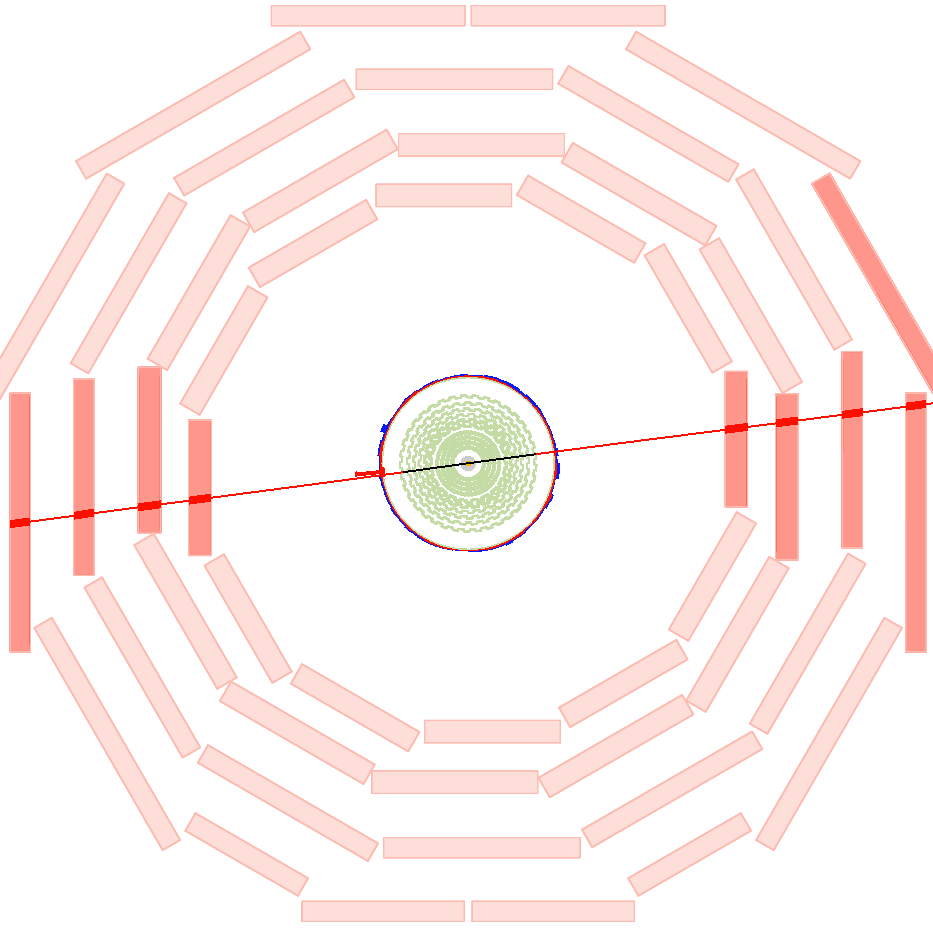
\includegraphics[width=0.99\textwidth]{figures/analysis/MotivationAndGeneralSearchStrategy/CharginoPairEvent_ctau_10000cm_lumi_1_event_12015.png}}
      \caption{}
  \end{subfigure} 
  \begin{subfigure}{0.31\textwidth}
    \frame{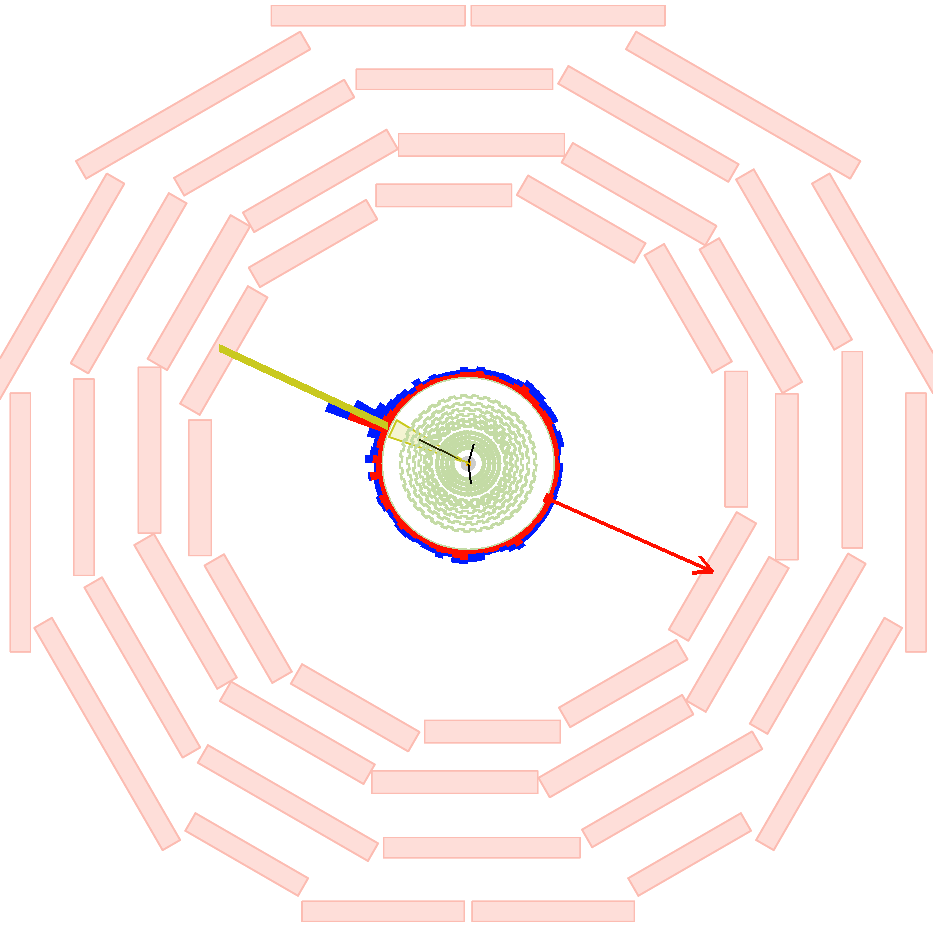
\includegraphics[width=0.99\textwidth]{figures/analysis/MotivationAndGeneralSearchStrategy/CharginoPairEvent_ctau_50cm_lumi_1_event_11024.png}}
      \caption{}
  \end{subfigure} 
  \begin{subfigure}{0.31\textwidth}
      \frame{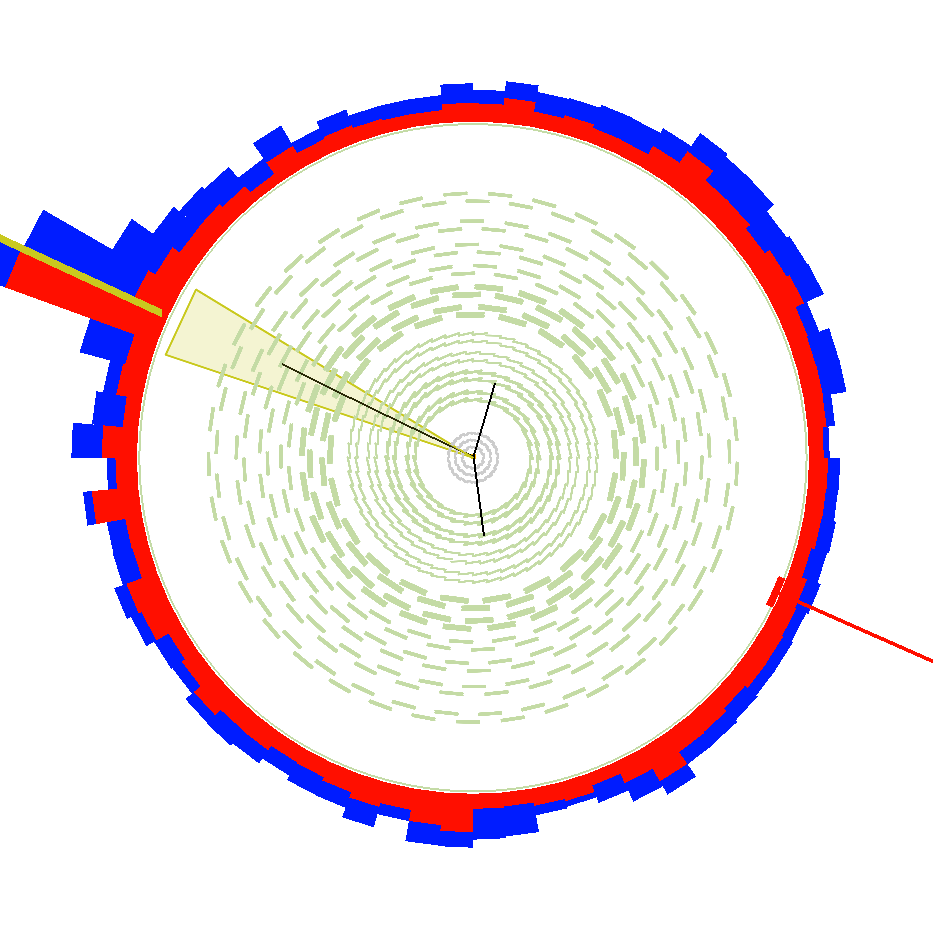
\includegraphics[width=0.99\textwidth]{figures/analysis/MotivationAndGeneralSearchStrategy/CharginoPairEvent_ctau_50cm_lumi_1_event_11024_Zoom.png}}
      \caption{}
  \end{subfigure} 
  \end{tabular}
  \caption{Visualisation of possible signatures of a chargino pair produced with a lifetime of $\ctau = 10\,\text{m}$ (a) and a lifetime of $\ctau = 0.5\,\text{m}$ (b and c). 
           The muon chambers are the outer layers of the detector and are depicted as red boxes.
           The black lines represent the reconstructed chargino tracks.
           The right picture (c) is a zoom of the middle picture (b). 
           Here, only the cross-section of the tracker (green wavy lines for the strip and grey lines for the pixel) is displayed. The red arrow shows the missing transverse energy in the event.
           The red (blue) towers correspond to the energy deposition in the ECAL (HCAL).
           The ISR jet in the middle and right picture is indicated as a yellow line.} 
  \label{fig:CharginoPaiEventDisplay}
\end{figure}
In the left picture of Fig.~\ref{fig:CharginoPaiEventDisplay}, both charginos are reconstructed as muons, which can be seen by the energy deposition in the muon chambers.
In the middle and right pictures both charginos have a lower lifetime of $\ctau=0.5\,$m and thus are only visible as tracks in the tracker, where both trajectories end inside the silicon strip tracker (by coincidence the tracks are equally long).
Since this analysis targets a search for Supersymmetry with charginos of lifetimes between $\ctau \approx 1\,\text{cm} - 10\,\text{cm}$, the charginos decay rather early in the detector, possibly even in the inner layers of the tracker.
%Thus, the signature of chargino events consists of isolated, short tracks that have large ionisation losses due to high chargino masses and the signatures of the decay products, \ie of a neutralino and a fermion pair. 
Thus, the signature of chargino events consists of isolated, short tracks and the signatures of the decay products, \ie of a neutralino and a fermion pair. 

In case of R-parity conservation, one of the chargino decay products, the neutralino, is stable and weakly interacting, thus traversing the detector without leaving any further signature.
%The missing transverse energy of the neutralino is balanced by the missing transverse energy of the second produced SUSY particle.
%This is either a neutralino or the decay products of the chargino in events with chargino pairs. 

The signature of the other decay product, the fermion pair, can in principle be used to select chargino events. 
However, for mass-degenerate charginos, it can be very hard or even impossible to detect these fermions as will be explained in detail in the next paragraph.

First of all, the fermionic decay product (\eg a pion) can usually not be reconstructed because it does not originate from the primary vertex.
Secondly, it is very low in momentum because of the mass-degeneracy between \chipm and \chiO.
The typical momentum of a pion originating from a chargino to neutralino decay in the \chipm rest frame is of the order 
\begin{equation}
p_{\pi}\sim \sqrt{ \left( m_{\chipm} - m_{\chiO} \right)^2 - m_{\pi}^2}.
\end{equation}
%As the \chipm is rather slow for higher masses this is a good approximation also in the detector rest frame.
For a mass gap between \chipm and \chiO of 150\mev, the \pt distribution of the resulting pion peaks \mbox{at $\sim$ 100\,\mev} and ends at \mbox{\pt $\sim 400\,$\mev} in the laboratory frame (Fig.~\ref{fig:ptOfPions}).
\begin{figure}[!t]
  \centering 
 \vspace{10pt}
  \begin{tabular}{c}
    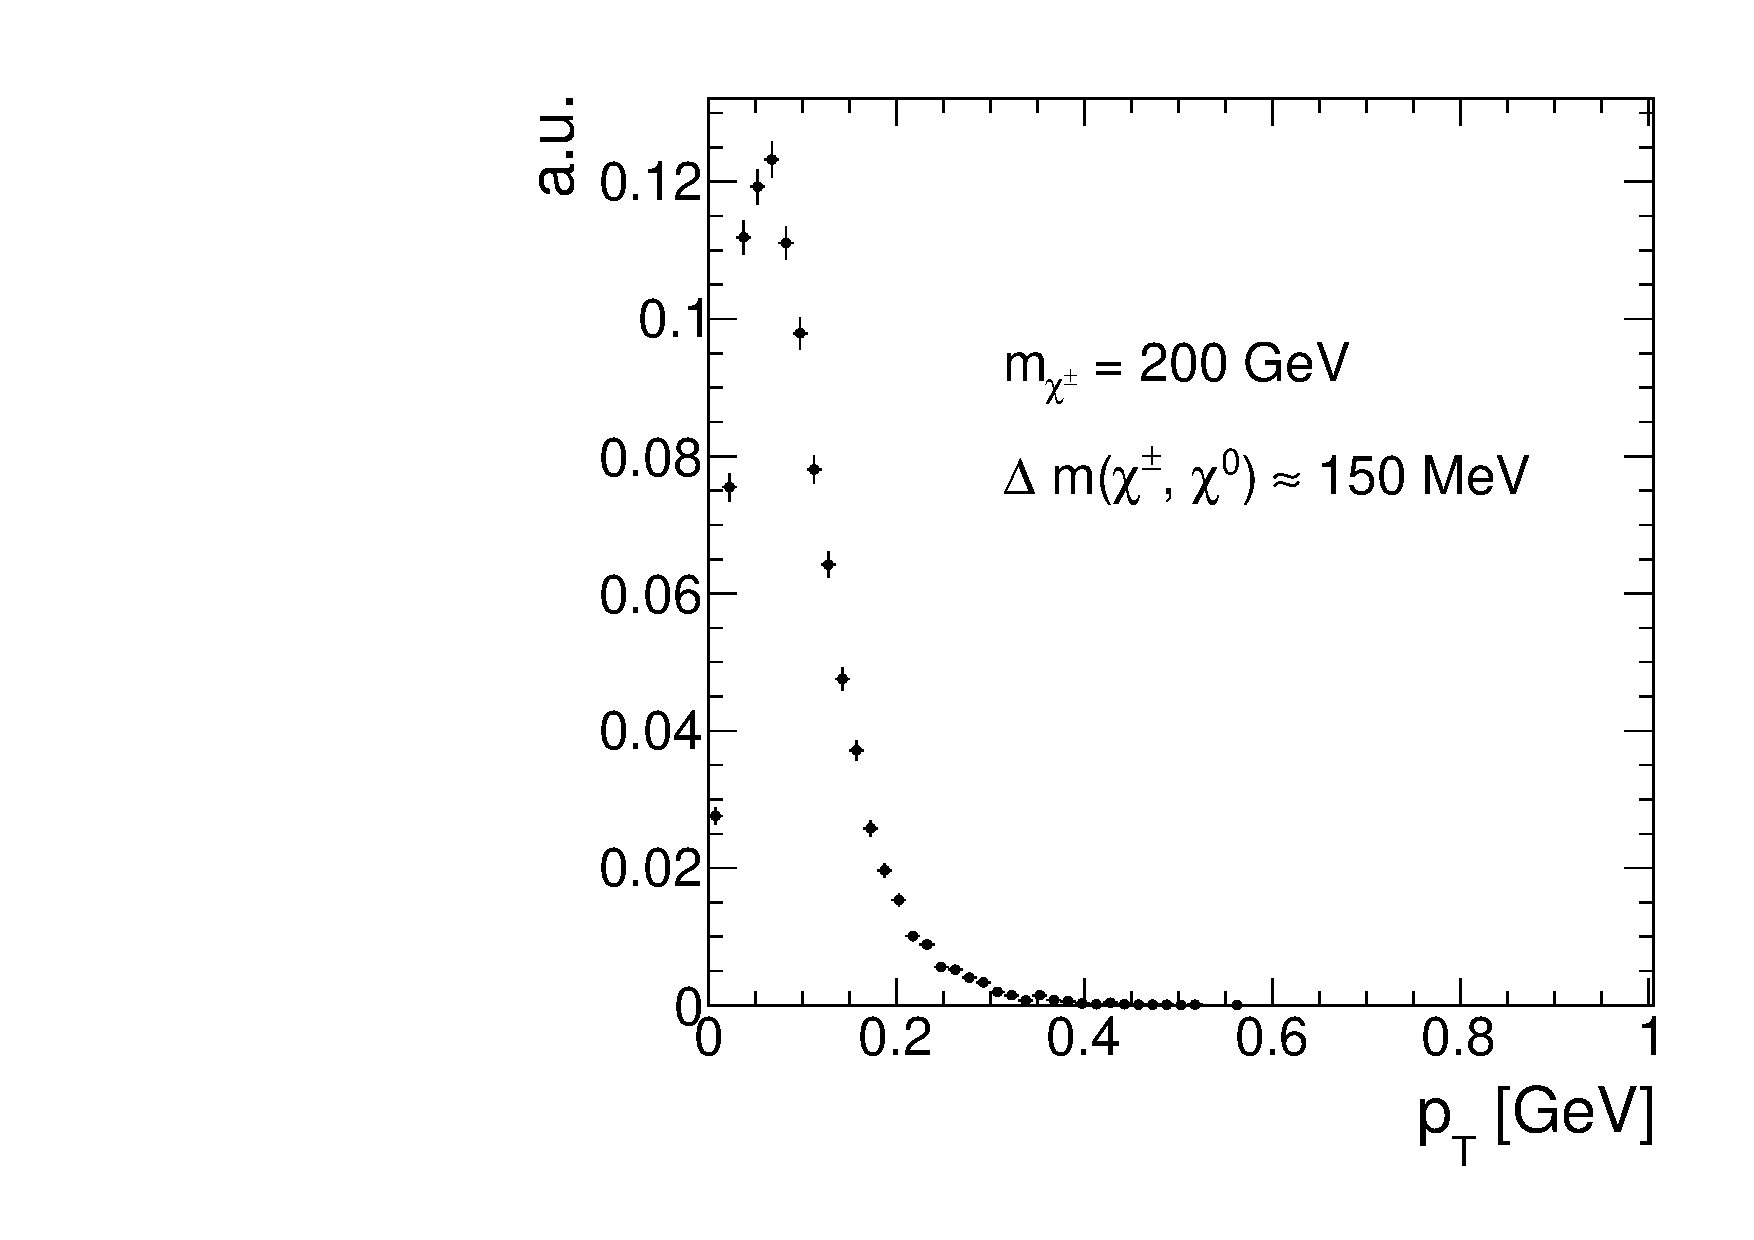
\includegraphics[width=0.49\textwidth]{figures/analysis/PtOfPions.pdf}
  \end{tabular}
  \caption{Transverse momentum distribution of pions coming from charginos decay into a neutralino with a mass gap of 150\mev.}
  \label{fig:ptOfPions}
\vspace{80pt}
\end{figure} 

If the transverse momentum of a particle is very low, the particle trajectory is much more bended compared to a particle with higher \pt (see Fig.~\ref{fig:KinkedTrack} for illustration).
Due to this bending, the track reconstruction efficiency of particles with a transverse momentum below 1\gev decreases rapidly, reaching around 40\% for isolated pions with a \pt of 100\mev~\cite{bib:CMS:tracking_8TeV}. 
Furthermore, for pions that are not produced in the primary vertex, this reconstruction efficiency will be even smaller.
It is therefore impossible to rely on a reconstruction of the fermionic chargino decay products in this analysis.
\begin{figure}[!b]
  \centering 
  \begin{tabular}{c}
    \frame{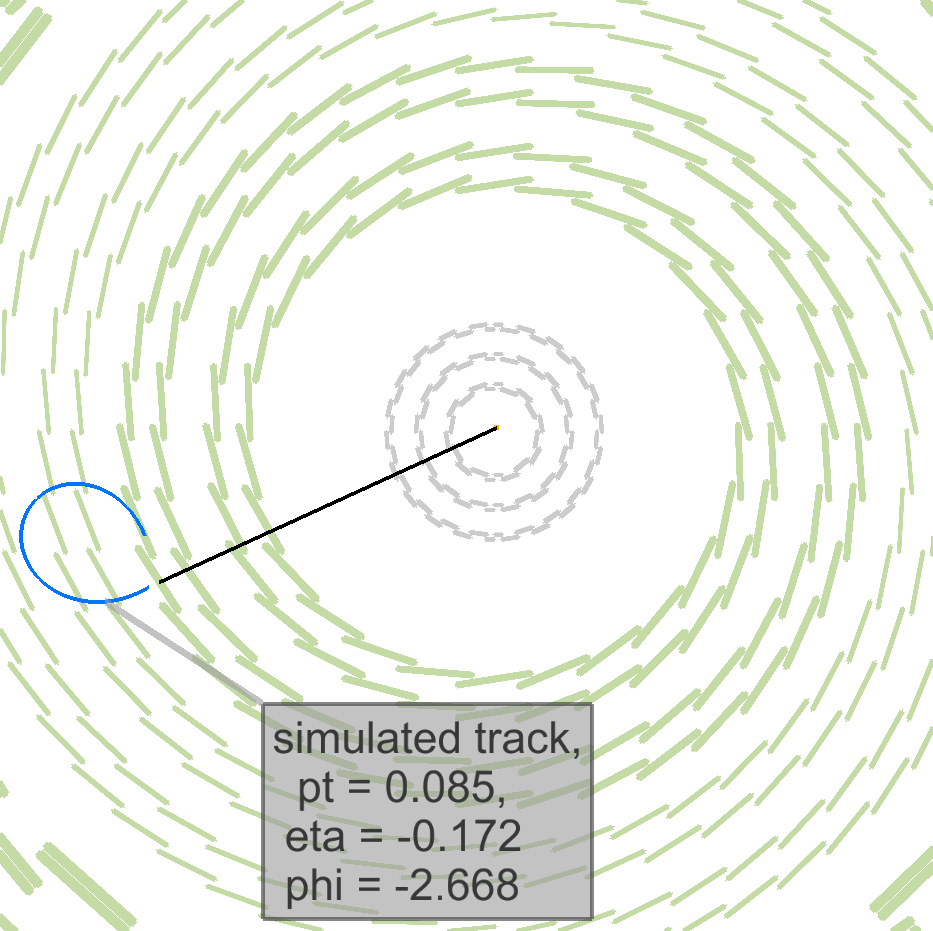
\includegraphics[width=0.4\textwidth]{figures/analysis/MotivationAndGeneralSearchStrategy/BendedPionTrack.png}}
    %\frame{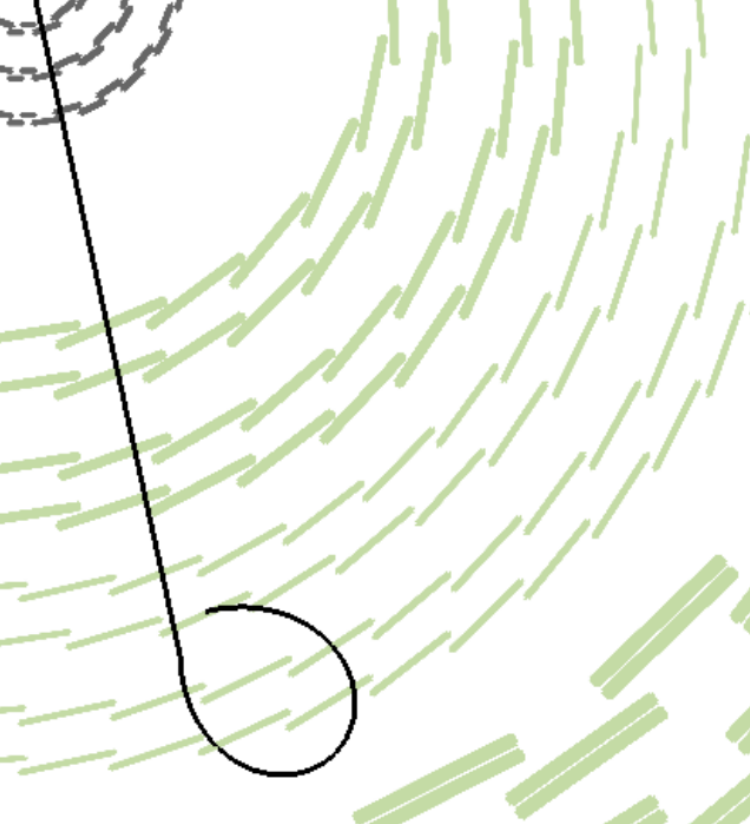
\includegraphics[width=0.30\textwidth]{figures/analysis/KinkedTrackZoom_Quadrat.png}}
  \end{tabular}
  \caption{Cross-sectional view of the silicon strip tracker (green lines) and silicon pixel tracker (grey lines). A simulated chargino track (black line) decays to a pion (bended blue line) with a \pt of $\sim 85\mev$ and a neutralino (not visible).}
  \label{fig:KinkedTrack}
\end{figure} 

In summary, since an early decaying chargino is not reconstructed as a PF particle, the event signature of a chargino-pair or a chargino-neutralino event consists only of one (or two) - potentially - disappearing track. 
Such a signature is very difficult to detect, especially since CMS doesn't offer a dedicated track trigger so that triggering on the chargino track is impossible.


In order to search for such signatures, one therefore needs to trigger on other, less obvious properties of chargino events. 
This analysis takes advantage of higher order contributions to the Feynman diagrams shown in Figs.~\ref{fig:FeynmanDiagramProductionCharginoPair} and~\ref{fig:FeynmanDiagramProductionCharginoNeutralino}, resulting in initial state radiation (ISR).
If the initial quarks radiate a high \pt gluon, the resulting jet can be detected and can offer a possibility to search for events with - apart from the ISR jet - nothing more than isolated tracks.
Furthermore, the non-detection of the chargino's decay products plus a high \pt ISR jet leads to missing transverse energy (MET) in the event. 
Exploiting these two circumstances, it is possible to detect chargino-pair or chargino-neutralino events with the help of Jet+MET triggers.

Since Jet+MET triggers are not very specific for chargino events, it is important to identify further track properties that can be used to select chargino candidates.
One distinctive property of charginos compared to SM particles is their high mass. 
Therefore, charginos can be identified by selecting high \pt tracks. 
Furthermore, the energy loss per path length (\dedx) depends quadratically on the particle's mass for low velocities ($0.2<\beta\gamma<0.9$):
\begin{equation}
\langle\frac{dE}{dx}\rangle = K \frac{m^2}{p^2} +C
\end{equation}
Therefore, \dedx constitutes a very nice discriminating variable for massive particles like charginos against SM particles.
The selection of chargino events in this analysis thus relies on the selection of isolated high \pt tracks with high \dedx values. 

If the chargino decays before it has crossed the full pixel and strip detector, the associated track is disappearing. 
For low lifetimes, the tracks can be very short and can have only a few hits in the detector. 
In order to reconstruct a particle's trajectory, a minimum of three hits are required since defining a helical path requires five parameters (see~\cite{bib:CMS:tracking_8TeV}). 
A specific challenge for this analysis is hence the combination of searching for short tracks and utilising the measurement of the energy deposition of the chargino. 
For very short tracks, eventually only passing the first couple of layers of the whole tracker system, the pixel tracker information becomes very important. 
Therefore, an accurate energy measurement in the pixel system is of great importance to this analysis. 
However, no other CMS analysis has used the energy information of the pixel tracker so far.
This analysis thus requires a thorough study of the quality of the pixel energy calibration and, potentially, a recalibration in case the pixel energy calibration is not sufficient.



\section{Comparison to earlier searches}
As already mentioned before, there are two analyses at CMS at $\sqrt{s}=8\,\tev$ with 20\fbinv data that search for intermediate lifetime charginos: the search for long-lived charged particles~\cite{bib:CMS:HSCP_8TeV} and the search for disappearing tracks~\cite{bib:CMS:DT_8TeV}.
The here presented analysis aims at achieving an increase in sensitivity towards shorter lifetimes compared to the earlier analyses in a twofold way.
First, the selection is optimised for the inclusion of very short tracks.
Second, the inclusion of the variable \dedx is used to increase the search sensitivity compared to~\cite{bib:CMS:DT_8TeV}.\\

In~\cite{bib:CMS:HSCP_8TeV}, a minimum number of eight hits were required for every track, whereas~\cite{bib:CMS:DT_8TeV} required a minimum of seven hits.
This can be very inefficient for shorter lifetimes, where most of the charginos already decay shortly after the pixel tracker.
In Fig.~\ref{fig:NHits_2Signal_noSelection_normalized} (left), the normalised distribution of the number of measurements (\nhits) of chargino tracks is shown. 
\begin{figure}[!b]
  \centering 
  \begin{tabular}{c}
  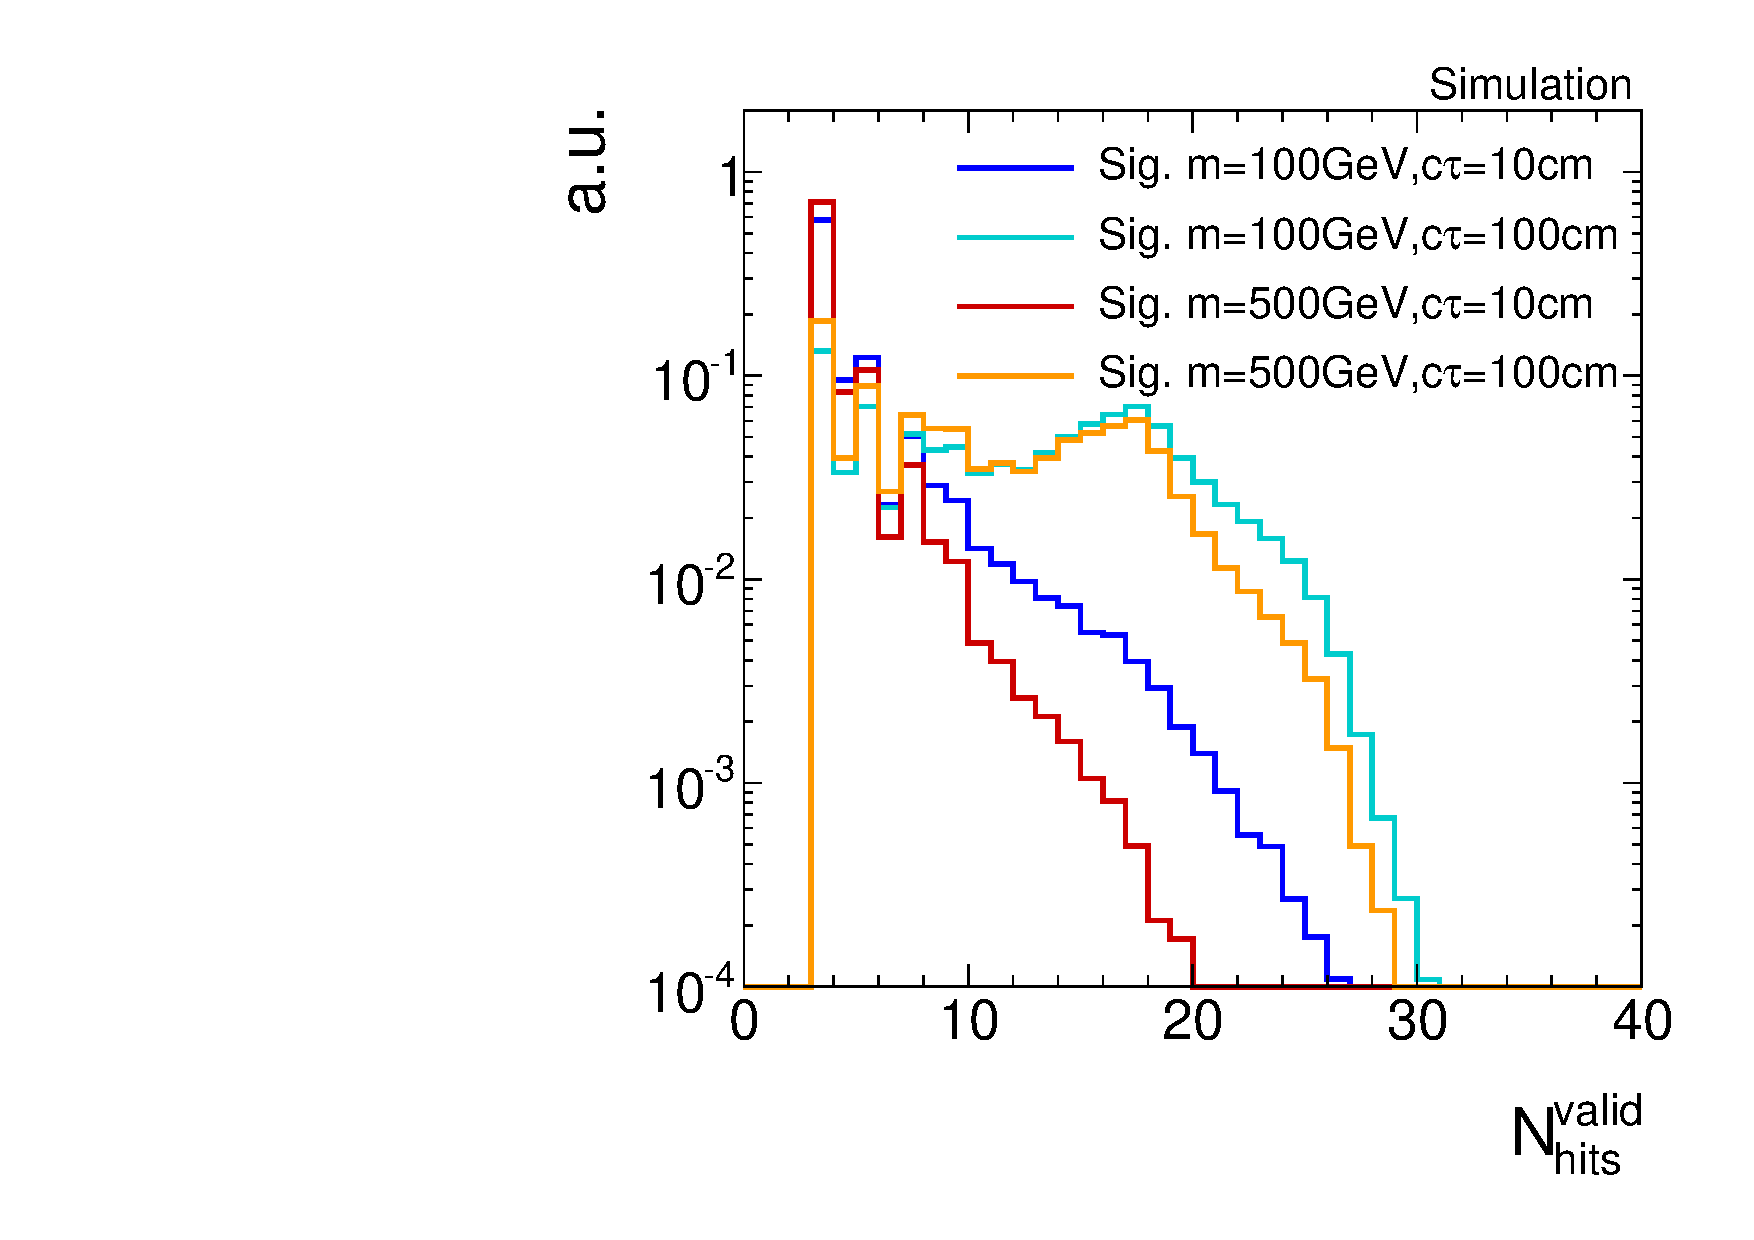
\includegraphics[width=0.49\textwidth]{figures/analysis_2/MotivationAndGeneralSearchStrategy/htrackNValid_log_chiTracksnoSelection.pdf}
  \includegraphics[width=0.49\textwidth]{figures/analysis_2/MotivationAndGeneralSearchStrategy/RecoEffTracksZoom.pdf}
  \end{tabular}
  \caption{Left: Number of measurements in the tracker system \nhits for four different signal lifetimes.
           Right: Probability to reconstruct a track (z) in dependency of the chargino's decay point (x and y).
           More information on the generation of the simulated signal samples can be found in Section~\ref{sec:SignalSamples}.} 
  \label{fig:NHits_2Signal_noSelection_normalized}
\end{figure}
It can be seen, that \nhits peaks at the minimal possible value needed for track reconstruction of $\nhits=3$ for lower lifetimes.
%For higher lifetimes ($\ctau=50\cm$) the distribution shifts to higher values with a second peak at $\nhits\sim17$.
For a lifetime of $\ctau=100\cm$, a second peak at $\sim$17 hits appears corresponding to the number of measurements when crossing all pixel barrel (3) and strip inner and outer barrel (6 from stereo and 8 from normal) layers.
However, a notable fraction of $\sim$ 40\% of chargino tracks still has a number of measurements of $\nhits<8$. 

It should also be mentioned that the track reconstruction efficiency is sufficient for short chargino tracks so that loosening the \nhits requirement is expected to really improve the signal acceptance. 
The track reconstruction efficiency for different chargino decay points is depicted in Fig.~\ref{fig:NHits_2Signal_noSelection_normalized} (right).
For very short tracks ($\nhits=3$) the efficiency is still around 20\%.



Additionally, the search for disappearing tracks which targets models with charginos decaying inside the tracker did not make use of the high energy deposition of heavy particles. 
Although this variable was indeed used in the search for long-lived charged particles, this search was not optimised for intermediate lifetimes (\eg no explicit muon veto on the selected tracks was required). 
Thus, it shows less sensitivity compared to the disappearing track search in the lifetime region between $10\,\text{cm} \lesssim c\tau \lesssim 100\,\text{cm}$ (see Fig.~\ref{fig:pMSSMplot}).\\

To conclude, the general search strategy of the here presented analysis is to unite the strategies of~\cite{bib:CMS:HSCP_8TeV} and~\cite{bib:CMS:DT_8TeV} and to lower the strong selection on the number of hits in these analyses in order to get an optimised selection for lifetimes around $1\,\text{cm} \lesssim c\tau \lesssim  30\,\text{cm}$.

%%%%%%%%%%%%%%%%%%%%%%%%%%%%%%%%%%%%%%%%%%%%%%%%%%%%%%%%%%%%%%%%%%%%%%%%%%%%%%%%%%%%%%%%%%%%%%%%%%%%%%%%%%%%%%%%%%%%%%%%%%%%%%%%%%%%%%%%%%%%%%%%%%%%%%%%%%%%%%%%%%%%%%%%%%%%%%%%%%%%
%%%%%%%%%%%%%%%%%%%%%%%%%%%%%%%%%%%%%%%%%%%%%%%%%%%%%%%%%%%%%%%%%%%%%%%%%%%%%%%%%%%%%%%%%%%%%%%%%%%%%%%%%%%%%%%%%%%%%%%%%%%%%%%%%%%%%%%%%%%%%%%%%%%%%%%%%%%%%%%%%%%%%%%%%%%%%%%%%%%%

%  %%%%%%%%%%%%%%%%%%%%%%%%%%%%%%%%%%%%%%%%%%%%%%%%%%%%%%%%%%%%%%%%%%%%%%%%%%%%%%%%%%%%%%%%%%%%%%%%%%%%%%%%%%%%%%%%%%%%%%%%%%%%%%%%%%%%%%%%%%%%%%%%%%%%%%%%%%%%%%%%%%%%%%%%%%%%%%%%%%%%
%%%%%%%%%%%%%%%%%%%%%%%%%%%%%%%%%%%%%%%%%%%%%%%%%%%%%%%%%%%%%%%%%%%%%%%%%%%%%%%%%%%%%%%%%%%%%%%%%%%%%%%%%%%%%%%%%%%%%%%%%%%%%%%%%%%%%%%%%%%%%%%%%%%%%%%%%%%%%%%%%%%%%%%%%%%%%%%%%%%%
%%%%%%%%%%%%%%%%%%%%%%%%%%%%%%%%%%%%%%%%%%%%%%%%%%%%%%%%%%%%%%%%%%%%%%%%%%%%%%%%%%%%%%%%%%%%%%%%%%%%%%%%%%%%%%%%%%%%%%%%%%%%%%%%%%%%%%%%%%%%%%%%%%%%%%%%%%%%%%%%%%%%%%%%%%%%%%%%%%%%
\FloatBarrier
\chapter{Improved dE/dx measurement for short tracks}
\label{sec:DeDxMeasurement}
As already pointed out in the previous chapter, the inclusion of the pixel energy measurements can increase the sensitivity when searching for short and highly ionising tracks.
While the energy measurements in the silicon strip detector have already been calibrated as part of the search for long-lived charged particles \cite{bib:CMS:HSCP_8TeV}, no complete calibration has been done for the pixel silicon tracker so far.
To increase the discrimination power of \dedx for short tracks, such a calibration procedure has therefore been performed within this PhD thesis.\\

The CMS tracker system provides a measurement of the particle's energy loss for each hit in the tracker.
This is done by the detection of the number of electrons produced by the ionisation of the silicon.
A detailed introduction to the CMS tracker system and the energy measurement can be found in Section~\ref{FIXME}.

How to combine the single energy measurements for each tracker hit into one track \dedx estimator that can be used for analysis purposes will be explained in the following Section~\ref{sec:sub:MeasuringDeDx}.
The pixel energy calibration is then described in Section~\ref{sec:EnergyCalibration}. 
How to discriminate SM particles and beyond SM particles with the help of a \dedx measurement is discussed in Section~\ref{sec:Ias}, followed by an exploration of how the inclusion of the pixel energy measurements in the \dedx estimates leads to a better discrimination between Standard Model particles and long-lived charginos (Section~\ref{sec:DiscriminationImprovements}).

%The CMS tracker system does not only allow for the precise measurement of particle tracks and primary and secondary vertices but also the measurement of a particle's mean energy loss per path length.
%This is done by the detection of the number of electrons produced by the ionisation of the particle during its passage through the silicon tracker.
%A detailed introduction to the CMS tracker system and the energy measurement can be found in Section~\ref{FIXME}.

%It was already pointed out that the inclusion of the pixel energy measurements can increase the sensitivity when searching for short and highly ionising tracks.
%While the silicon strip detector has already been calibrated as part of the search for long-lived charged particles \cite{bib:CMS:HSCP_8TeV}, no complete calibration has been done for the pixel silicon tracker so far.
%To increase the discrimination power of \dedx for short tracks, such a calibration procedure is therefore conducted within this PHD thesis.


\section{Estimation of the ionisation loss of charged particles}
\label{sec:sub:MeasuringDeDx}
Energy losses for moderately relativistic charged particles travelling through matter are mostly caused by ionisation effects.
The mean energy loss per path length can be described with the Bethe formula \cite{bib:Bethe_1930}:
\begin{equation}
\langle \frac{dE}{dx} \rangle = Kz^2\frac{Z}{A}\frac{1}{\beta^2} [ \frac{1}{2} \ln{\frac{2m_e c^2 \beta^2 \gamma^2 T_{\text{max}}}{I^2}} - \beta^2 - \frac{\delta( \beta \gamma )}{2} ].
\end{equation}
It is a function of the atomic number ($Z$), the atomic mass ($A$) of the absorber, and the mean excitation energy ($I$) which is 173\,eV for silicon~\cite{bib:NIST}.  
$T_{\text{max}}$ represents the maximum energy transfer in a single collision.
The relevant particle's properties are the velocity ($\beta$), the Lorentz factor ($\gamma$) and the charge (z) of the incident particle.
The density correction $\delta( \beta \gamma )$ reduces the mean energy loss at high energies because of polarisation effects of the material. 
%The constant factor K is $4\pi N_A r_e^2 m_e^2 c^2$ with $N_A$ being the Avogadro constant, $m_e$ the electron mass and $r_e$ the classical electron radius of 2.8\,fm.
The factor K is constant and is 0.307 in units of $\mev\,$mol$^{-1}$cm$^2$.
The Bethe formula is valid if the main energy loss originates from ionisation effects, \ie in a region between $0.1\lesssim\beta\gamma\lesssim 1000$.


Even if widely used, the mean energy loss is a quantity which is ``ill-defined experimentally and is not useful for describing energy loss by single particles'' \cite{bib:PDG_2014}.
The problem is caused by the underlying probability distribution of one single \dedx measurement (this will be named $\Delta E/ \Delta x $ throughout the following sections), which can be parametrised by a Landau distribution \cite{bib:Landau_1944}
\begin{equation}
p(x) = \frac{1}{\pi} \int_0^\infty\! e^{-t \log t - x t} \sin(\pi t)\, dt.
\end{equation}
The Landau distribution has no free parameters. Its most probable value is around 0.222.
However, it is possible to introduce artificially a different most probable value and a width (at half maximum) with $x \rightarrow \frac{x-\text{MPV}}{\sigma}-0.222$.
The Landau distribution is a highly asymmetric distribution with a long tail towards large $x$ values (see Fig.~\ref{fig:landau}).
\begin{figure}[!t]
  \centering 
  \begin{tabular}{c}
  \includegraphics[width=0.49\textwidth]{figures/analysis/PixelCalibration/Landau.pdf}
  \end{tabular}
  \caption{Illustration of the shape of a Landau distribution. Parameters were chosen as $\mu=200$ and $\sigma=20$.} 
  \label{fig:landau}
\end{figure}
Theoretically it extends to infinite energies, however in nature the maximal deposited energy is of course limited by the particle's full energy.
%The mean and the variance of a landau distribution are not defined.

Because of its strong asymmetry, measurements of the mean energy loss per path length $\langle \dedx \rangle$ with only a few single measurements are easily fluctuating towards high values.
This makes the use of the mean energy loss described by the Bethe formula for the discrimination of new heavy particles problematic, because fluctuations to high values reduce the discrimination power against massive particles which release in general higher amounts of energy in matter.
%This is again different for a (limited) measurment, as there it is always possible to calucalute a mean.
%Still, this leads to the fact that the definition of the mean energy loss per path length is a problematic and unstable concept.


A much better observable is the most probable value (MPV) of the Landau distribution.
The MPV is much more stable compared to the mean and is not subject (FIXME) to high \dedx fluctuations. 
The most probable energy loss of a charged particle, $\Delta_p$, can be described by the Landau-Vavilov-Bichsel equation \cite{bib:Bichsel:MPV_1988}:
\begin{equation}
\Delta_p = \xi \left[ \ln \frac{2m_e c^2\beta^2\gamma^2}{I}  + \ln\frac{\xi}{I} + j - \beta^2 - \delta(\beta\gamma)  \right],
\label{eq:Landau_Vavilov_Bichsel}
\end{equation}
with $\xi=(K/Z)\langle Z/A \rangle (x/\beta^2)$. 
The thickness of the absorber $x$ appears explicitly in the Landau-Vavilov-Bichsel equation making the most probable energy loss per path \mbox{length $\Delta_p/dx$} logarithmically dependent on $x$.
A comparison between the Bethe mean energy loss $\langle \dedx \rangle$ and the most probable energy loss $\Delta_p/dx$ for muons is shown in Fig.~\ref{fig:dEdx_Bethe_Landau}.

%However, it is difficult to determine the most probable value for tracks with only a few energy measurements available.
%Large fluctuations can still lead to a bias towards higher value of the most probable \dedx.

Particles such as  muons are minimally ionising in silicon for $\beta\gamma \sim 3-4$. 
For higher momenta the deposited energies increase again reaching a plateau at around $\beta\gamma\sim100$. 
However, new heavy charged particles would mainly be unrelativistic because of their high mass and would therefore deposit much higher energies in the detector.
This makes \dedx  a very well discriminating variable.
%\begin{figure}[!bt]
%  \centering 
%  \begin{tabular}{c}
%  \includegraphics[width=0.6\textwidth]{figures/analysis/dEdx_Landau_Silicon.png}
%  \end{tabular}
%  \caption{Most probable energy loss in silicon, scaled to the mean loss of a minimally ionising particle (388 eV/$\mu$m) for different absorber thicknesses. Taken from \cite{bib:PDG_2014}.} 
%  \label{fig:dEdx_Landau_Silicon}
%\end{figure}
\begin{figure}[!t]
  \centering 
  \begin{tabular}{c}
  \includegraphics[width=0.6\textwidth]{figures/analysis/dEdx_Bethe_Landau.png}
  \end{tabular}
  \caption{Comparison between the Bethe mean energy loss, restricted energy loss and the most probable energy loss described by the Landau-Vavilov-Bichsel function for muons for different values of absorber thickness of silicon. Taken from \cite{bib:PDG_2014}.} 
  \label{fig:dEdx_Bethe_Landau}
\end{figure}
Thus, the energy loss per path length can be used to discriminate between SM particles and new heavy charged particles due to the different velocity distributions.\\



As said before, the most probable energy loss is much more stable compared to the Bethe mean energy loss.
Still, combining only a few measurements of $\Delta E/\Delta x$ can also lead for $\Delta_p/dx$ to large fluctuations towards high \dedx values.
In order to estimate experimentally the most probable \dedx value from only a few energy measurements, several ``estimators'' can be used that suppress a potential bias towards the high end without introducing a bias towards lower values~\cite{bib:Quertenmont_2010}.
One of the estimators for determining a track's \dedx is the harmonic-2 estimator
\begin{equation}
\ihtwo=\left( \frac{1}{N}\sum_{i=1}^{N}(\Delta E_i/\Delta x_i)^{-2} \right)^{-1/2},
\label{eq:Harmonic2Estimator}
\end{equation}
where $\Delta E_i /\Delta x_i$ corresponds to the $\Delta E$ and $\Delta x$ measurement in the $i$th hit of the track. 
This estimator is known to be robust and is not easily biased by large fluctuations in  $\Delta E/\Delta x$ because of the suppression by the power of minus two~\cite{bib:Quertenmont_2010}.
%The harmonic mean of all $N$ measurements to the power of two is used as estimator for the MPV of the \dedx distribution of a particle.

A further estimator of \dedx used for the discrimination of highly ionising particles will be introduced in Section~\ref{sec:Ias}.


\FloatBarrier
\section{Energy calibration of the silicon pixel tracker}
\label{sec:EnergyCalibration}
During Run I in 2012, the pixel silicon detector was continuously subjected to an energy calibration, a so-called gain calibration.
Every pixel was calibrated to the same response, so that the whole pixel tracker should have been well inter-calibrated~\cite{bib:Danek}.
Unfortunately, due to various reasons, such as the imperfect constancy of the reference signal, or radiation and temperature induced changes, the energy calibration could not ensure a fully calibrated pixel tracker.
%was not adequate enough to use the measured energy deposition without a further offline calibration procedure.

This imperfection of the gain calibration can be seen in Fig.~\ref{fig:StabilityPlot_beforeCalibration}, where the mean of the harmonic-2 estimator for all tracks $\langle\ihtwo \rangle$ over the full data-taking period in 2012 is shown.
Four different steps can be spotted.
\begin{figure}[!b]
  \centering 
  \begin{tabular}{c}
  \includegraphics[width=0.49\textwidth]{figures/analysis/PixelCalibration/StabilityPlot_Pixel_beforeCalibration_withoutStepFits_NEW.pdf}
  \end{tabular}
  \caption{Mean of all track's \dedx (harmonic-2 estimator) over the full year 2012. Only pixel hits are taken into account. Every data point corresponds to one run.} 
  \label{fig:StabilityPlot_beforeCalibration}
\end{figure}
The first and the third steps correspond to changes in the settings of the tracker due to irradiation.
The second and fourth step are induced by associated adjustments in the online gain calibration.
Unfortunately, although the gain calibration was adjusted (even with some delay), it was not able to ensure a constant energy response of the pixel tracker over time. 
The variations of the \dedx measurement over time of around 15\% are too large to use \dedx without a further calibration. 

The following sections explain the method of the gain calibration of the pixel silicon tracker which is performed for this analysis. 
It is splitted into two sections. 
The first section is dedicated to the gain inter-calibration of the pixel tracker which ensures a homogeneous energy response of all tracker modules.
In the second section, the absolute gain calibration is discussed. 
This calibration step is needed to ensure that the measurement of the energy release of a particle is actually translated to the correct physical value.

%Detailed technical information about the pixel tracker can be found in Section~\ref{sec:Detector:Pixel}.


\subsection*{Inter-calibration of gain}
The main goal of the gain calibration is to get a uniform response in the ionisation energy loss \dedx over the full data taking period in 2012.
To also ensure a uniform response over all modules within one time step, an additional inter-calibration on module level is carried out.
The inter-calibration can in principle be done on various levels: the highest granularity would be a calibration on pixel level, followed by a calibration on read-out-chip (ROC) level and then on module-level.
Lower granularities in descending order are rings (modules with same z-position) and finally layers (3 layers in the barrel and 4 disks in the endcap). 
It is verified that all pixels~\cite{bib:Danek} and all ROCs (on one module) are sufficiently inter-calibrated, such that the inter-calibration is finally done module-wise.
For the pixel inter-calibration it is relied on~\cite{bib:Danek}, whereas the spread of derived calibration factors of all ROCs within one module was analysed to be around 5\% for most of the pixel modules (see Fig.~\ref{FIXME} in Appendix{FIXME}). FIXME:talk to Markus

%The applied method for the gain calibration of the pixel tracker closely follows the method in \cite{bib:Quertenmont_2010}.

The gain calibration of the pixel silicon tracker is carried out with the help of minimally ionising particles (MIPs).
MIPs in this context are not defined as particles at the minimum of the Bethe formula, but more generally as particles located at or near the plateau of the \dedx distribution vs. momentum (see Fig.~\ref{fig:dEdx_Bethe_Landau}).
This approach ensures that all particles deposit similar amounts of energy so that the variation due to different momenta is minimised.

MIPs are selected by a momentum selection of $\text{p}>2\,$\gev.
Additionally, only tracks with at least eight hits and a $\chi^2/\text{n.d.o.f.}<3$ are used to ensure a high-quality track reconstruction.
A sample containing around $~$50 million ``minimum bias'' events is used for calibration.
The ``minimum bias'' sample was specifically recorded for tracker calibration purposes.
%Its distinctive property is that neither an online nor offline selection was applied.

For every module in the pixel tracker (there are 1440 modules in total), a distribution of the energy loss per path length $\Delta E/\Delta x$ is built.
The measurement of $\Delta E/\Delta x$ is done in ADC counts per mm.
ADC counts are a measure for the deposited charge after digitisation.
%each $\Delta E/\Delta x$  measurement of all particles crossing the module is filled into a histogram. 
Figure~\ref{fig:dEdx_Module} shows an example distribution for one module. 
\begin{figure}[!t]
  \centering 
  \begin{tabular}{c}
  \includegraphics[width=0.49\textwidth]{figures/analysis/Landau_Module_352476680.pdf}
  \end{tabular}
  \caption{An example of the $\Delta E/\Delta x$ distribution measured in ADC count per mm for one module of the CMS pixel tracker. 
           A Landau convoluted with a Gaussian is fitted to the core of the distribution in an iterative procedure.} 
  \label{fig:dEdx_Module}
\end{figure}
The underlying Landau distribution can be seen. 
To extract the MPV for every module a fit to the core distribution is performed.
The fit is not only done with a Landau but a Landau convoluted with a Gaussian function to be closer to the experimentally observed energy spectrum.
This also increases the fit performance and the stability of the fit.
The path length $\Delta x$ is calculated with
\begin{equation}
\Delta x = d_{\text{module}_i} \cdot \cos(\phi_{\text{track}}),
\end{equation}
where $d_{\text{module}_i}$ is the thickness of module i and $\phi_{\text{track}}$ is the relative angle of the particle's trajectory to the normal axis of the module.
With the measured MPV extracted from the fit, an inter-calibration factor is calculated for every module
\begin{equation}
c_{\text{inter}}=\frac{\mpv_{\text{target}}\, [\text{ADC/mm}]}{\mpv\, [\text{ADC/mm}]} = \frac{300 \cdot 265 \, \text{ADC/mm}}{\mpv\, [\text{ADC/mm}]}.
\end{equation}
The factor 300 $\cdot$ 265 ADC/mm is in principal an arbitrary number since the final response is adjusted by the absolute gain calibration described in the next section.
However, it is chosen such that the measured calibration factors are close to one.
The calibration factor can then be used to scale every single measurement in a module to a calibrated $\Delta E/\Delta x$ measurement
\begin{equation}
\left( \frac{\Delta E}{\Delta x}\right)_{\text{calibrated}}=c_{\text{inter}} \cdot \left(\frac{\Delta E}{\Delta x}\right)_{\text{uncalibrated}}
\end{equation}
The determination of the calibration factor is done for every of the five time steps, shown in Fig.~\ref{fig:StabilityPlot_beforeCalibration} independently, in order to get rid of the time dependency. 
The outcome of the application of the calibration factors to the single energy measurements in the pixel tracker can be seen in Fig.~\ref{fig:StabilityPlot_afterCalibration}.
The variation over time is indeed eliminated, resulting in a maximal time variation of less than $\sim1$\%.

\begin{figure}[!t]
  \centering 
  \begin{tabular}{c}
  \includegraphics[width=0.49\textwidth]{figures/analysis/PixelCalibration/StabilityPlot_Pixel_afterCalibration_withoutStepFits_NEW.pdf}
  \end{tabular}
  \caption{Mean of all track's \dedx (harmonic-2 estimator) over the full year 2012 after applying the calibration factors, resulting in an average \dedx of 3.51 MeV/cm. Only pixel hits are taken into account. Every data point corresponds to one run.} 
  \label{fig:StabilityPlot_afterCalibration}
\end{figure}


Additionally, the same procedure is carried out for a corresponding simulated data sample to ensure the inter-calibration of the pixel modules on all simulated samples.



\subsection*{Absolute calibration of gain}
As a final step, the targeted \mpv being $\mpv_{\text{target}}=300 \cdot 265 \,  \text{ADC/mm}$ needs to be translated to a meaningful physical quantity given in physical units (\eg MeV/cm).
That means, that the charge measurement in ADC counts needs to be converted to the real energy release from a particle.
The relation between $\Delta E$ in ADC counts and the energy loss in eV is given by
\begin{equation}
\Delta E\,[\ev] = c_{\text{inter}} \cdot \Delta E\,[\text{ADC}] \cdot \frac{N_e}{\text{ADC}} \cdot 3.61 \, \ev,
\end{equation}
where $N_e$/ADC is the number of electrons which correspond to one calibrated ADC count and 3.61\,\ev is the  mean energy needed to create one electron-hole pair in silicon at $-10\degree$C.
Such an absolute gain calibration can be done with the help of several methods (all explained in \cite{bib:Quertenmont_2010}).
The absolute calibration of the silicon pixel tracker can rely on the already performed/accomplished FIXME  absolute calibration of the silicon strip detector.
In \cite{bib:Quertenmont_2010}, the absolute gain calibration was done with the help of the most probable energy release per path length of muons, 
theoretically described by the Landau-Vavilov-Bichsel formula in Eq.~\eqref{eq:Landau_Vavilov_Bichsel}.  
To calibrate the pixel tracker to the correct energy loss per path length it is therefore sufficient to determine one calibration factor to relate the average \dedx of all tracks in the pixel tracker as shown in 
Fig.~\ref{fig:StabilityPlot_afterCalibration} to the average measured \dedx in the strip tracker, shown in Fig.~\ref{fig:StabilityPlot_Strip} by
\begin{equation}
c_{\text{absolute}} = \frac{\langle dE/dx_{\text{strip}} \rangle}{\langle dE/dx_{\text{pixel}} \rangle} = \frac{3.303}{3.509} = 0.941.
\end{equation}
\begin{figure}[!t]
  \centering 
  \begin{tabular}{c}
  \includegraphics[width=0.49\textwidth]{figures/analysis/PixelCalibration/StabilityPlot_Strip_afterCalibration_withoutStepFits_NEW.pdf}
  \end{tabular}
  \caption{Mean of all track's \dedx (harmonic-2 estimator) measured in the silicon strip detector over the full year 2012. The average most probable \dedx is $\ihtwo=3.303\,\mev/\cm$. Every data point corresponds to one run.} 
  \label{fig:StabilityPlot_Strip}
\end{figure}
This factor is then applied on top of $c_{\text{inter}}$ for all pixel modules.

Finally, an absolute calibration factor needs to be determined for the simulated samples, where the simulated pixel tracker is calibrated to the average \dedx of the silicon strip measured in data.


\section{Discrimination of highly-ionising particles}
\label{sec:Ias}

As mentioned before, it is difficult to find a robust estimator for the most probable energy loss of a particle, if only a few measurements of $\Delta E/ \Delta x$  along the particle's trajectory are available.
The harmonic-2 estimator \ihtwo was already introduced in Section~\ref{sec:sub:MeasuringDeDx} in Eq.~\eqref{eq:Harmonic2Estimator}.
It is known to be a robust estimator not easily affected by large fluctuations in $\Delta E/ \Delta x$.
However, it was shown in \cite{bib:Quertenmont_2010} that a better discrimination between SM particles and possible new heavy particles can be achieved when using likelihood techniques,
\ie determining the probability that the set of all $\Delta E/ \Delta x$ belonging to one track is actually compatible with the hypothetical probability distribution of a MIP.

That a measured sample has been drawn from a specific distribution can be tested with the co-called Smirnov-Cram\'{e}r-von Mises test~\cite{bib:Anderson:CramerVonMises_1962,bib:James:StaticticalMethods_2006}.
%It is deduced from the integral of the squared difference of the measured distribution $P_N(x)$ to the hypothesis distribution $P(x)$
It is deduced from the integral of the squared difference of a measured distribution to a hypothesis distribution, 
%\begin{equation}
%I_s = \int\limits_{-\infty}^{\infty} \left[P_{N}(x)-P(x)\right]^2 dP(x)
%\end{equation}
and leads to a test statistics of~\cite{bib:Quertenmont_2010}
\begin{equation}
I_s = \frac{3}{N} \cdot \left( \frac{1}{12N} + \sum\limits_{i=1}^N \left[ P_i - \frac{2i-1}{2N} \right]^2 \right),
\end{equation}
where N is the total number of energy measurements and $P_i$ is the cumulative probability that a MIP would release a $\Delta E/\Delta x$ equal or smaller than the measured $\Delta E/ \Delta x$ with all $P_i$ arranged in increasing order.

However, this test statistics is not sensitive to the sign of the difference between the measured and the theoretical distribution.
It can therefore not distinguish between incompatibilities due to variations towards higher or lower energy deposits compared to the hypothesis distribution.
Thus it is not optimal for the discrimination between MIPs and heavy new particles by \dedx.
A so-called Asymmetric Smirnov-Cram\'{e}r-von Mises discriminator was developed in \cite{bib:Quertenmont_2010} which is only sensitive to incompatibilities to the MIP hypothesis towards higher energy depositions
\begin{equation}
\ias = \frac{3}{N} \cdot \left( \frac{1}{12N} + \sum\limits_{i=1}^N \left[ P_i \cdot \left(P_i - \frac{2i-1}{2N} \right)^2 \right] \right).
\end{equation}
A value of \ias close to zero indicates good compatibility with the MIP hypothesis, whereas a value close to one indicates bad compatibility because of unexpectedly high energy losses.

The underlying probability P$_i$ of the energy release for a given path length in the pixel tracker is extracted from the same ``minimum bias'' sample used for the pixel energy calibration.
In total 28 different templates each for a different given path length are created.
In Fig.~\ref{fig:ProbabilityTemplate} the probability distribution template for the pixel tracker in data and simulation is shown.
The corresponding templates for the energy release in the silicon strip detector were already built by  \cite{bib:Quertenmont_2010}.


A comparison between the energy release by MIPs (\ias) in data and simulation for high-quality tracks with $p>5\gev$ and $|\eta|<2.1$ can be found in Fig.~\ref{fig:Data-MC-Dedx_MIPs}.
\begin{figure}[!b]
  \centering 
  \begin{tabular}{c}
    \includegraphics[width=0.49\textwidth]{figures/analysis_2/PixelCalibration/Discriminator_template_data_pixel_2012.pdf}
    \includegraphics[width=0.49\textwidth]{figures/analysis_2/PixelCalibration/Discriminator_template_mc_pixel_2012.pdf}
  \end{tabular}
  \caption{Cumulative probability for a MIP to release a $\Delta E/ \Delta x$ (y-axis) vs. the path length (x-axis) in data (left) and simulation (right) for the pixel tracker based on the ``minimum bias'' sample.}
 % \vspace{60pt}
  \label{fig:ProbabilityTemplate}
\end{figure}

\begin{figure}[!bt]
%\vspace{10pt}
  \centering 
  \begin{tabular}{c}
    \includegraphics[width=0.49\textwidth]{figures/analysis_2/PixelCalibration/htrackASmiSmallRange_log_MIPs.pdf}
  \end{tabular}
  \caption{Normalised \ias distribution for MIPs from the minimum bias sample in data and simulation for high-quality (high purity as defined in \cite{bib:CMS:Tracking_2010}, a minimum number of eight hits and no missing inner and middle hits) tracks with $p>5\gev$ and $|\eta|<2.1$.}
  \label{fig:Data-MC-Dedx_MIPs}
\end{figure}
\dedx shows good agreement in data and simulation for $\ias<0.1$.
For larger values, \ias shows a larger decrease in simulation than in measured data.
For this reason a data-based approach for analyses exploiting \dedx information is needed.\\

\section{Discrimination improvements}
\label{sec:DiscriminationImprovements}
The goal of including the pixel energy information is to increase the discrimination power of \ias between background and signal tracks, especially for shorter lifetimes.
In Fig.~\ref{fig:MIPs-Signal-Dedx} (left), a comparison of the shapes of the energy release by MIPs and by signal tracks in simulation is shown (details about the simulated samples can be found in the next section Section~\ref{sec:SignalSamples}).
\begin{figure}[!t]
  \centering 
  \begin{tabular}{c}
    \includegraphics[width=0.49\textwidth]{figures/analysis_2/PixelCalibration/htrackASmiSmallRange_log_chiTracksGoodQualitySelection_2Signal_ttjets.pdf}   
    \includegraphics[width=0.49\textwidth]{figures/analysis_2/PixelCalibration/htrackASmiSmallRange_log_chiTracksGoodQualitySelection_4Signal.pdf}
  \end{tabular}
  \caption{Normalised \ias distribution for simulated background and signal tracks (left) and for four different signal models (right) 
           for high-purity tracks (as defined in \cite{bib:CMS:Tracking_2010}) with \pt$>10\gev$ and $|\eta|<2.1$.
           For the illustration of the background tracks' spectrum simulated $t\bar{t}$+jets events are used (more information about this sample is given in Chapter~\ref{ch:SimulatedSamples}).}
  \label{fig:MIPs-Signal-Dedx}
\end{figure} 
It can be seen, that the \ias distributions of the signal models show a larger tail towards $\ias=1$, whereas the \ias of the background is rapidly falling.

In the right part of Fig.~\ref{fig:MIPs-Signal-Dedx}, a comparison of the \ias distributions of four different signal models is shown.
Charginos with longer lifetimes have a more pronounced tail toward $\ias=1$.
This can be understood with the help of Eq.~\eqref{eq:Landau_Vavilov_Bichsel}, where the influence of the velocity ($\beta$) on the ionisation loss can be seen.
The velocity distribution of the charginos is mostly affected by the mass of the chargino.
However, also for charginos with same mass, the velocity is higher in average for shorter lifetimes.
This is caused by the fact, that for shorter lifetimes (\eg $\ctau=10\cm$), already a sizable fraction of the charginos decay before reaching the tracker system.
The probability of reaching the detector increases for higher velocities because of the boost, which can be clearly seen at the survival probability
\begin{equation}
P \left( t \right) = e^{-\frac{t}{\gamma \tau}}.
\end{equation} 
This means that the track reconstruction/selection lead to a biased average $\beta$ for shorter lifetimes which in turn lead to lower values of \ias.

The \ias distribution is not only influenced by the velocity of a particle but also by the number of hits of a track.
The number of measurements in the tracker system defines the influence of single fluctuations in $\Delta E/\Delta x$ on the \ias discriminator, because of the long right tail of the Landau distribution.
A low number of hits, therefore, leads to higher \ias values.
This effect is also visible in Fig.~\ref{fig:MIPs-Signal-Dedx} (right). 
The small surplus for lower lifetimes between 0.1 and 0.2 is caused by the smaller number of measurements for earlier decaying charginos.

%Thus, \ias for charginos with lower lifetimes are affected by two things: 
%First, due to the smaller number of measurements the chargino tends to higher \ias values.
%Second, low lifetimes charginos have in average a higher velocity leading to lower \ias values.
%Both effects can be seen in Fig.~\ref{fig:MIPs-Signal-Dedx} (right).
%The large tail for longer lifetimes is caused by the lower velocities, but the small surplus for lower lifetimes between 0.1 and 0.2 is caused by the smaller number of measurements for earlier decaying charginos.\\


Finally, the impact of the additional $\Delta E/\Delta x$ information from the pixel tracker on the selection efficiency of signal and background tracks is quantified.
Figure~\ref{fig:ROCplots} shows the signal selection efficiency against the background selection efficiency for different selection cuts in \ias, once including the pixel information and once without it.
\begin{figure}[!t]
  \centering 
  \vspace{50pt}
  \begin{tabular}{c}
    \includegraphics[width=0.49\textwidth]{figures/analysis/rocplot_wjets_mass_100GeV_ctau_5cm.pdf} 
    \includegraphics[width=0.49\textwidth]{figures/analysis/rocplot_wjets_mass_100GeV_ctau_50cm.pdf} \\
    \includegraphics[width=0.49\textwidth]{figures/analysis/rocplot_wjets_mass_500GeV_ctau_5cm.pdf} 
    \includegraphics[width=0.49\textwidth]{figures/analysis/rocplot_wjets_mass_500GeV_ctau_50cm.pdf}
  \end{tabular}
  \caption{Signal selection efficiency vs. background selection efficiency with (red) and without (black) pixel information.
           Each point correspond to one selection cut in \ias.
           The figure is based on a simulated \WJets sample and a simulated signal sample with chargino-chargino production, both subject to a selection of high-quality tracks (without a selection on \nhits) with $\pt>10\gev$.}
  \vspace{40pt}
  \label{fig:ROCplots}
\end{figure} 
The background selection efficiency is estimated with simulated $W$+jets  events but was additionally checked on simulated $t\bar{t}$+jets  and QCD-multijet events 
(further information about the simulated samples can be found in the next Chapter~\ref{ch:SimulatedSamples}).
No significant difference between these processes in the background selection efficiency was observed.

The signal selection efficiency and the background suppression depend on the mass and the lifetime of the charginos.
The improvement of the discriminating power is much more pronounced for higher chargino masses.

It can be seen that the inclusion of the pixel information increases the background suppression for a given signal efficiency throughout the investigated signal models.
This background suppression improvement is most pronounced for very tight cuts on \ias up to a factor of 20 and even more and still considerable for looser selections with signal efficiencies of around 40\% (factor of 10).
%%%%%%%%%%%%%%%%%%%%%%%%%%%%%%%%%%%%%%%%%%%%%%%%%%%%%%%%%%%%%%%%%%%%%%%%%%%%%%%%%%%%%%%%%%%%%%%%%%%%%%%%%%%%%%%%%%%%%%%%%%%%%%%%%%%%%%%%%%%%%%%%%%%%%%%%%%%%%%%%%%%%%%%%%%%%%%%%%%%%
%%%%%%%%%%%%%%%%%%%%%%%%%%%%%%%%%%%%%%%%%%%%%%%%%%%%%%%%%%%%%%%%%%%%%%%%%%%%%%%%%%%%%%%%%%%%%%%%%%%%%%%%%%%%%%%%%%%%%%%%%%%%%%%%%%%%%%%%%%%%%%%%%%%%%%%%%%%%%%%%%%%%%%%%%%%%%%%%%%%%

%  %%%%%%%%%%%%%%%%%%%%%%%%%%%%%%%%%%%%%%%%%%%%%%%%%%%%%%%%%%%%%%%%%%%%%%%%%%%%%%%%%%%%%%%%%%%%%%%%%%%%%%%%%%%%%%%%%%%%%%%%%%%%%%%%%%%%%%%%%%%%%%%%%%%%%%%%%%%%%%%%%%%%%%%
%%%%%%%%%%%%%%%%%%%%%%%%%%%%%%%%%%%%%%%%%%%%%%%%%%%%%%%%%%%%%%%%%%%%%%%%%%%%%%%%%%%%%%%%%%%%%%%%%%%%%%%%%%%%%%%%%%%%%%%%%%%%%%%%%%%%%%%%%%%%%%%%%%%%%%%%%%%%%%%%%%%%%%%
%%%%%%%%%%%%%%%%%%%%%%%%%%%%%%%%%%%%%%%%%%%%%%%%%%%%%%%%%%%%%%%%%%%%%%%%%%%%%%%%%%%%%%%%%%%%%%%%%%%%%%%%%%%%%%%%%%%%%%%%%%%%%%%%%%%%%%%%%%%%%%%%%%%%%%%%%%%%%%%%%%%%%%%

\FloatBarrier
\chapter{Simulated samples}
\label{ch:SimulatedSamples}

In order to design the search and to study background and signal characteristics, this analysis relies on simulated  SM and SUSY datasets.
An extensive introduction to the techniques and tools required for the simulation of SM and beyond SM processes can be found in Section~\ref{FIXME}.

The following two sections present an overview of the SM (Section~\ref{sec:SMSamples}) and SUSY samples (Section~\ref{sec:SignalSamples}) used in this search.
All samples are reweighted to match the measured distribution of primary vertices per event in data.
Additionally, event weights are applied to ensure the same ISR spectrum in simulation as in data.

%%%%%%%%%%%%%%%%%%%%%%%%%%%%%%%%%%%%%%%%%%%%%%%%%%%%%%%%%%%%%%%%%%%%%%%%%%%%%%%%%%%%%%%%%%%%%%%%%%%%%%%%%%%%%%%%%%%%%%%%%%%%%%%%%%%%%%%%%%%%%%%%%%%%%%%%%%%%%%%%%%%%%%%
\section{Standard Model background samples}
\label{sec:SMSamples}
To investigate the sources of background, various simulated SM samples are used.
Since this analysis aims at making use of \dedx, a special data format of the simulated samples, the so-called RECO format, is required.
Unfortunately, not all SM processes are available in this specific format making it impossible to compare the total number of events in simulation and real data.
This, however, does not constitute a serious problem since this analysis will finally use data-based background estimation methods.
The simulated SM datasets can still be used to compare the shapes of important distributions in simulation and data.\footnote{For example, the simulated \ZInvJets sample that can contribute to the background of this search via fake tracks is not available in RECO format. However, as the shape of important observables of fake tracks is independent of the underlying process, this background can be studied with a simulated \WJets sample.}
Still, the most important SM background sample including \WJets events is available.
Due to the intrinsic missing energy in \WJets events it constitutes the major background to the presented search (see Section~\ref{ch:BackgroundEstimation} for further details on the backgrounds). \\

In Table \ref{tab:SMsamples_RECO} all available SM samples used in this analysis are listed.
The matrix-elements of the \WJets, \ttbarJets and \ZlepJets samples are generated using \madgraph5~\cite{bib:Madgraph_2014}. 
For the QCD sample \pythiaSix~\cite{bib:Pyhtia6_2006} is used for generation.
All samples are then passed to \pythia6 to simulate the hadronisation and the showering. %, the underlying event and the beam remnants.
The interactions between the particles and the detector material is simulated using \geant~\cite{bib:Geant4_2003,bib:Geant4_2006}.

%\renewcommand{\arraystretch}{1.5}
%\begin{table}[!h]
%\centering
%\caption{Available Standard Model background samples containing $\Delta E/\Delta x$ information that are used for background estimation studies.}
%\label{tab:SMsamples_RECO}
%\makebox[0.99\textwidth]{
%\begin{tabular}{lll}
%\multicolumn{3}{c}{} \\
%\toprule
% Process & Cross section $\left[\pb\right]$ & $\mathcal{O}_{\text{calculation}}^{\text{cross section}}$ \\%& Size $\left[\text{TB}\right]$\\
%\midrule
% \WJets                                                &  36703.2      &  NNLO \cite{bib:FEWZ} \\%& 70.4 \\
% \ttbarJets                                            &  245.8        &  NNLO \cite{bib:ttbar:Czakon_2013}\\%& 55.9 \\
% \ZlepJets ($\ell=e,\mu,\tau$)                         &  3531.9       &  NNLO \cite{bib:FEWZ} \\%& 5.1  \\
% QCD ($50\gev<\hat{p}_{\text{T}}<1400\gev$)               &  9374794.2    &  LO  \\%% & 44.3\\
%\bottomrule
%\multicolumn{3}{c}{} \\
%\end{tabular}}
%\end{table}

Due to the size of the samples (between 5 and 70\,TB per sample) a reduction is required in order to limit the storage space requirements.
This is achieved by selecting only events which contain at least one jet with a minimum transverse momentum of $\pt>60\gev$.

In addition, further simulated samples not containing \dedx information are used (so-called AOD samples).
Because of their much smaller size, these samples are available in full size.
They are needed to study the background inclusively in the variable \dedx.

\renewcommand{\arraystretch}{1.5}
\begin{table}[!h]
\centering
\caption{Available Standard Model background samples containing $\Delta E/\Delta x$ information that are used for background estimation studies.}
\label{tab:SMsamples_RECO}
\makebox[0.99\textwidth]{
\begin{tabular}{llll}
\multicolumn{4}{c}{} \\
\toprule
 Process & Generator & Cross section $\left[\pb\right]$ & $\mathcal{O}_{\text{calculation}}^{\text{cross section}}$ \\%& Size $\left[\text{TB}\right]$\\
\midrule
 \WJets                                        &   \madgraph5     &  36703.2      &  NNLO \cite{bib:FEWZ} \\%& 70.4 \\
 \ttbarJets                                    &   \madgraph5     &  245.8        &  NNLO \cite{bib:ttbar:Czakon_2013}\\%& 55.9 \\
 \ZlepJets ($\ell=e,\mu,\tau$)                 &   \madgraph5     &  3531.9       &  NNLO \cite{bib:FEWZ} \\%& 5.1  \\
 QCD ($50\gev<\hat{p}_{\text{T}}<1400\gev$)      &   \pythia6      &  9374794.2    &  LO  \\%% & 44.3\\
\bottomrule
\multicolumn{4}{c}{} \\
\end{tabular}}
\end{table}  

%They are listed in Table~\ref{tab:SMsamples_AOD}.
%\renewcommand{\arraystretch}{1.5}
%\begin{table}[!h]
%\centering
%\caption{Standard Model background samples without $\Delta E/\Delta x$ information.}
%\label{tab:SMsamples_AOD}
%\makebox[0.99\textwidth]{
%\begin{tabular}{lll}
%\multicolumn{3}{c}{} \\
%\toprule
% Process & Cross section $\left[\pb\right]$ & $\mathcal{O}_{\text{calculation}}$ \\%& Size $\left[\text{TB}\right]$\\
%\midrule
%\WJets                                             &  36703.2    &  NNLO \cite{bib:FEWZ} \\%& 70.4 \\
%\ZlepJets ($\ell=e,\mu,\tau$)                      &  3531.9     &  NNLO \cite{bib:FEWZ} \\%& 5.1  \\
%\bottomrule
%\multicolumn{3}{c}{} \\
%\end{tabular}}
%\end{table}  

%%%%%%%%%%%%%%%%%%%%%%%%%%%%%%%%%%%%%%%%%%%%%%%%%%%%%%%%%%%%%%%%%%%%%%%%%%%%%%%%%%%%%%%%%%%%%%%%%%%%%%%%%%%%%%%%%%%%%%%%%%%%%%%%%%%%%%%%%%%%%%%%%%%%%%%%%%%%%%%%%%%%%%%
\section{Signal samples}
\label{sec:SignalSamples}
For the investigation of a possible SUSY signal, events containing either chargino pair production $q\bar{q} \rightarrow \chipm \chimp$ or chargino neutralino production $q\bar{q} \rightarrow \chipm \chiO$ are simulated within this thesis. 
The simulation of the samples is done as described in Section~\ref{sec:SMSamples} for the \WJets sample.
%The simulation is done with the matrix-element event generator \madgraphFive~\cite{bib:Madgraph_2014}.
%The parton showering and hadronisation processes are then simulated with \pythiaSix~\cite{bib:Pyhtia6_2006}.
%Finally, the interactions of the generator-level particles with the detector material are simulated  with \geant~\cite{bib:Geant4_2003,bib:Geant4_2006}.
However, a special treatment for long-lived particles is required for this analysis.
In order to get a correct detector simulation of the energy loss of long-lived particles that decay after the beam pipe, the decay of the chargino cannot be simulated within \madgraph or \pythia but needs to be simulated within \geant.
The decay mode of the chargino is also specified within \geant to a neutralino plus pion decay, $ \chipm \rightarrow \chiO\, \pi^{\pm}$.

To reduce the required computing sources, the simulation is only done for a few lifetimes (\ctau = 1\cm, 5\cm, 10\cm, 50\cm, 100\cm, 1\,000\cm and 10\,000\cm).
The lifetime is hereby not controlled by changing the mass gap between the chargino and the neutralino but is independently specified within \geant.
In order to scan in a high resolution over the lifetime space, other lifetimes are generated using lifetime reweighting.
The weight for each event depends on the individual proper lifetime of the chargino and is given by
\begin{equation}
w = \prod_{i=1}^n \frac{\tau^{\text{gen}}}{\tau^{\text{target}}}\cdot  \exp \left[ t_i \cdot \left( \frac{1}{\tau^{\text{gen}}} - \frac{1}{\tau^{\text{target}}} \right) \right] ,
\end{equation}
where $n$ is the  number of charginos in the event, $\tau^{\text{gen}}$ is the generated mean lifetime in the particle's rest frame and $t_i$ is the individual proper lifetime of the chargino. 
The targeted mean lifetime is given by $\tau^{\text{target}}$. 
A derivation of this formula can be found in Appendix~\ref{app:LifetimeReweighting}.
Using this reweighting procedure a good coverage of the lifetime space can be achieved with lifetimes of $1\cm \leq \ctau \leq 10^4 \cm $. %\ctau = $a\cdot10^{n}$ for $n=0,1,2,3$ and $a=\left[1,9\right]$.
Figure~\ref{fig:LifetimeReweighting} shows the exponential distribution of the individual proper lifetime of the charginos after the reweighting of a simulated sample with $c\tau^{\text{gen}}=50\cm$ to a lifetime of $c\tau^{\text{target}}=10\cm$.
\begin{figure}[!b]
  \centering 
  \begin{tabular}{c}
    \includegraphics[width=0.49\textwidth]{figures/analysis_2/10cm.pdf}
  \end{tabular}
  \caption{Normalised distribution of the proper individual lifetime $d_{\text{lab}}/\left(\beta\gamma \right)$ of all charginos contained in a signal sample with a generated lifetime of $c\tau^{\text{gen}}=50\cm$ reweighted to a lifetime of $c\tau^{\text{target}}=10\cm$. Fitting an exponential curve $a\cdot \exp\left[\frac{1}{c \tau } c t_i\right]$ yields $c\tau=\text{slope}^{-1}=10\cm$.}
  \label{fig:LifetimeReweighting}
\end{figure}
It can be seen that the reweighting procedure does indeed reproduce the targeted lifetime of 10\cm.


All samples are generated for different masses of the chargino, but always almost mass-degenerate to the lightest neutralino.
The mass gap between chargino and neutralino is set to 150\mev and, as said before, is hereby disentangled to the chargino lifetime for the simulation of the signal samples.
However, since this analysis does not make use of the decay products of the chargino and the mass gap is for all simulated lifetimes of a similar small size, the choice of the mass gap does not affect the signal prediction.
Six different masses from 100\gev to 600\gev are simulated.
This leads to a total number of 42 signal samples.
In Table~\ref{tab:SignalCrossSections}, the cross sections at $\sqrt{s}=8\tev$ for $\chipm\chimp$ and $\chipm\chiO$ production for wino-like charginos and neutralinos are listed~\cite{bib:SignalCrossSection_2012,bib:SignalCrossSection_2013}.
The cross section does not depend on the lifetime of the chargino.
\renewcommand{\arraystretch}{1.5}
\begin{table}[h]
\centering
\caption{Simulated signal mass points with corresponding cross sections at NLO-NLL (NLO: next-to-leading order, NLL: next-to-leading logarithmic) accuracy for wino-like charginos~\cite{bib:SignalCrossSection_2012,bib:SignalCrossSection_2013}.}
\label{tab:SignalCrossSections}
\makebox[0.99\textwidth]{
\begin{tabular}{lll}
\multicolumn{3}{c}{} \\
\toprule
 $m_{\chipm}\left[\gev\right]$ & $\sigma_{\chipm\chimp}\left[\pb\right]$  & $\sigma_{\chiO\chimp}\left[\pb\right]$ \\
\midrule
 100     &  5.8234     &  11.5132 \\
 200     &  0.37924    &  0.77661 \\
 300     &  0.06751    &  0.14176 \\
 400     &  0.01751    &  0.03758 \\
 500     &  0.00553    &  0.01205 \\
 600     &  0.00196    &  0.00431 \\
\bottomrule
\multicolumn{3}{c}{} \\
\end{tabular}}
\end{table}  

%%%%%%%%%%%%%%%%%%%%%%%%%%%%%%%%%%%%%%%%%%%%%%%%%%%%%%%%%%%%%%%%%%%%%%%%%%%%%%%%%%%%%%%%%%%%%%%%%%%%%%%%%%%%%%%%%%%%%%%%%%%%%%%%%%%%%%%%%%%%%%%%%%%%%%%%%%%%%%%%%%%%%%%%%%%%%%%%%%%%
%%%%%%%%%%%%%%%%%%%%%%%%%%%%%%%%%%%%%%%%%%%%%%%%%%%%%%%%%%%%%%%%%%%%%%%%%%%%%%%%%%%%%%%%%%%%%%%%%%%%%%%%%%%%%%%%%%%%%%%%%%%%%%%%%%%%%%%%%%%%%%%%%%%%%%%%%%%%%%%%%%%%%%%%%%%%%%%%%%%%

%  %%%%%%%%%%%%%%%%%%%%%%%%%%%%%%%%%%%%%%%%%%%%%%%%%%%%%%%%%%%%%%%%%%%%%%%%%%%%%%%%%%%%%%%%%%%%%%%%%%%%%%%%%%%%%%%%%%%%%%%%%%%%%%%%%%%%%%%%%%%%%%%%%%%%%%%%%%%%%%%%%%%%%%%%%%%%%%%%%%%%
%%%%%%%%%%%%%%%%%%%%%%%%%%%%%%%%%%%%%%%%%%%%%%%%%%%%%%%%%%%%%%%%%%%%%%%%%%%%%%%%%%%%%%%%%%%%%%%%%%%%%%%%%%%%%%%%%%%%%%%%%%%%%%%%%%%%%%%%%%%%%%%%%%%%%%%%%%%%%%%%%%%%%%%%%%%%%%%%%%%%
\FloatBarrier
\chapter{Event selection}
\label{sec:EventSelection}
\section{Datasets and triggers}
\label{sec:DatasetsAndTriggers}

The analysis is performed on $pp$-collision data recorded in the year 2012 by the CMS experiment at a centre-of-mass energy of $\sqrt{s}=8\tev$.
In total an integrated luminosity of 19.7\fbinv was recorded in 2012.

As outlined in Section~\ref{sec:GeneralSearchStrategy}, the detection of chargino tracks is a challenging task already on trigger level.
Direct triggering of events containing chargino-like tracks is not possible because in 2012 there was no dedicated track trigger available.
Furthermore, there is no intrinsic missing transverse energy in the event if the chargino is not reconstructed as a PF particle, \eg when it decays inside the tracker.
Therefore, this analysis uses initial state radiation for the detection of chargino events.
If ISR occurs, it is possible to trigger on a high-\pt jet (\ptfirstjet) and missing transverse momentum (\met).

For this purpose, several triggers are utilised in this analysis.
An event is selected, if at least one of the three triggers in Table~\ref{tab:triggers} fired.
The \seqsplit{HLTMonoCentralPFJet80\_{PF}\-{MET}\-noMu95\_NHEF0p95} and HLTMonoCentralPFJet80\_PFMETnoMu105\_NHEF0p95 triggers both rely on the L1 ETM40 trigger which requires the missing energy to be larger than 40\gev.
On HLT level, they further require at least one particle-flow jet within the pseudorapidity range of $|\eta|<2.6$ with $\pt>80\gev$ and the PF missing transverse momentum (not taking into account the \pt of muons) to be larger than 95\gev or 105\gev, respectively.
Finally, no more than 95\% of the jet energy must be carried by neutral hadrons.
The HLTMonoCentralPFJet80\_PFMETnoMu95\_NHEF0p95 trigger was active during Run\,A and Run\,B in 2012 data taking, whereas HLTMonoCentralPFJet80\_PFMETnoMu105\_NHEF0p95 was in place during Run\,C and Run\,D in 2012.

%
%To consider the event in the analysis, at least one of them must have fired.
%In Table~\ref{tab:triggers} the three triggers are listed together with the corresponding recorded integrated luminosity in the time when they were active.
\renewcommand{\arraystretch}{1.5}
\begin{table}[!t]
\centering
\caption{\met and \met+ jet triggers used in this analysis together with the corresponding recorded integrated luminosity during the time when they were in place.}
\label{tab:triggers}
\makebox[0.99\textwidth]{
\begin{tabular}{lr}
\multicolumn{2}{c}{} \\
\toprule
Trigger  & Integrated luminosity [\fbinv]   \\
\midrule
 HLTMonoCentralPFJet80\_PFMETnoMu95\_NHEF0p95     &  5.3   \\
 HLTMonoCentralPFJet80\_PFMETnoMu105\_NHEF0p95    &  14.4  \\
 HLT\_MET120\_HBHENoiseCleaned                    &  19.7  \\
\bottomrule
\multicolumn{2}{c}{}
\end{tabular}}
\end{table}  

The HLT\_MET120\_HBHENoiseCleaned trigger is based on the L1 trigger ETM36. % that are combined by a logical OR.
On HLT level, the trigger requires that the missing energy measured from calorimeter energy deposits is larger than 120\gev.
The HBHENoise-filter reduces background from electronic noise in the HCAL.
This trigger was active during the full data taking period in 2012.

\renewcommand{\arraystretch}{1.5}
\begin{table}[!b]
\centering
\caption{MET data samples used in the search with the contained integrated luminosity.}
\label{tab:SearchSamples}
\makebox[0.99\textwidth]{
\begin{tabular}{lr}
\multicolumn{2}{c}{} \\
\toprule
Dataset  & Integrated luminosity [\fbinv]   \\
\midrule
 /MET/Run2012A-22Jan2013-v1/RECO         &  0.876   \\
 /MET/Run2012B-22Jan2013-v1/RECO         &  4.412  \\
 /MET/Run2012C-22Jan2013-v1/RECO         &  7.055  \\
 /METParked/Run2012D-22Jan2013-v1/RECO   &  7.354  \\ 
\bottomrule
\multicolumn{2}{c}{}
\end{tabular}}
\end{table} 
The events that were selected by the described triggers are available in the MET datasets listed in Table~\ref{tab:SearchSamples}. 
Again, because of the size of the datasets ($\sim150\,$TB in total), a reduction of the size is achieved by selecting only events where one of the used triggers fires and that contains at least one jet with a minimum \pt of 50\gev.
This reduction in size of almost 80\% is necessary to make this analysis technically feasible.


%In addition, the analysis makes use of the datasets listed in Table~\ref{tab:ControlSamples}.
%These datasets are used for background estimation purposes and the estimation of their associated systematic uncertainties.
%\renewcommand{\arraystretch}{1.5}
%\begin{table}[!hbt]
%\centering
%\caption{Further datasets used for background estimation.}
%\label{tab:ControlSamples}
%\makebox[0.99\textwidth]{
%\begin{tabular}{lr}
%\multicolumn{2}{c}{} \\
%\toprule
%Dataset  & Luminosity [\fbinv]   \\
%\midrule
%/SingleMu/Run2012A-22Jan2013-v1/AOD        &  0.876 \\
%/SingleMu/Run2012B-22Jan2013-v1/AOD        &  4.405 \\
%/SingleMu/Run2012C-22Jan2013-v1/AOD        &  7.040 \\
%/SingleMu/Run2012D-22Jan2013-v1/AOD        &  7.369 \\ 
%\midrule
%/SingleElectron/Run2012A-22Jan2013-v1/AOD  &  0.876 \\
%/SingleElectron/Run2012B-22Jan2013-v1/AOD  &  4.412 \\
%/SingleElectron/Run2012C-22Jan2013-v1/AOD  &  7.050 \\
%/SingleElectron/Run2012D-22Jan2013-v1/AOD  &  7.368 \\
%\bottomrule
%\end{tabular}}
%\end{table}  
%%%%%%%%%%%%%%%%%%%%%%%%%%%%%%%%%%%%%%%%%%%%%%%%%%%%%%%%%%%%%%%%%%%%%%%%%%%%%%%%%%%%%%%%%%%%%%%%%%%%%%%%%%%%%%%%%%%%%%%%%%%%%%%%%%%%%%%%%%%%%%%%%%%%%%%%%%%%%%%%%%%%%%%%%%%%%%%%%%%%
\section{Selection of signal candidate events}
\label{sec:AnalysisSelection}

In order to suppress events originating from Standard Model processes such as QCD-multijet events, \WJets, etc., a selection favouring signal-like tracks is applied.
The signal candidate selection closely follows the selection required in the disappearing track search~\cite{bib:CMS:DT_Thesis,bib:CMS:DT_8TeV_AN}.
It relies on event-based and track-based variables as described in the following two sections.


\subsection{Event-based selection}
\label{sec:EventBasedSelection}
First, a selection on the quality of the primary vertex is applied in order to suppress cosmic events and noise from the beam halo.
This selection includes requirements on the position of the vertex with respect to the beam axes and the number of degrees of freedom of the vertex which is strongly correlated to the number of tracks originating from the vertex (see~\cite{bib:CMS:Tracking_7TeV_PAS} for further details):  
\begin{itemize}
\renewcommand{\labelitemi}{\footnotesize{\ding{118}}}
\item The vertex must have at least four degrees of freedom: \mbox{$vtx$ with $\geq 4$ d.o.f.}
\item The position of the vertex along the beam line must be within 24\cm with respect to the nominal interaction point: \mbox{$|dz| \leq 24\cm$.}
\item The position in the transverse direction must be within 2\cm with respect to the nominal interaction point: \mbox{$|d0| \leq 2\cm$.}\\
\end{itemize}
%After these selection cuts are applied the remaining events are subjected to a further preselection.\\

To maximise the signal acceptance, the trigger related selection cuts are chosen close to the trigger thresholds (see Section~\ref{sec:DatasetsAndTriggers}).
In Fig.~\ref{fig:SignalMET+SignalJetPt}, the distributions of \met and the transverse momentum of the leading jet, \ptfirstjet, are shown for different signal models.
\begin{figure}[!t]
  \centering 
  \begin{tabular}{c}
    \includegraphics[width=0.49\textwidth]{figures/analysis/AnalysisSelection/hMetSmallRange_log_chiTracksnoSelection_4Signals.pdf}
    \includegraphics[width=0.49\textwidth]{figures/analysis/AnalysisSelection/h1stjetptSmallRange_log_chiTracksnoSelection_4Signals.pdf}
  \end{tabular}
  \caption{Normalised distributions of the missing transverse momentum (left) and the transverse momentum of the leading jet (right) for four different signal models.}
  \label{fig:SignalMET+SignalJetPt}
\end{figure}
The leading jet has to be centrally produced, $|\eta_{\text{\nth{1}jet}}|<2.4$, and to fulfil the following criteria: %Only jets with $|\eta|<2.4$ that fulfil the following further criteria are taken into account:
\begin{itemize}
\item Charged hadron energy fraction (CHF$_{\text{\nth{1}jet}}$) $>0.2$
\item Charged electromagnetic energy fraction (CEF$_{\text{\nth{1}jet}}$) $<0.5$
\item Neutral hadron energy fraction (NHF$_{\text{\nth{1}jet}}$) $<0.7$
\item Neutral electromagnetic energy fraction (NEF$_{\text{\nth{1}jet}}$) $<0.7$.
\end{itemize}
These additional jet quality criteria ensure that noise from cosmic and beam halo muons and high-\pt photons and electrons is suppressed \cite{bib:CMS:DM_8TeV_AN}.

The trigger efficiency as a function of \met and \ptfirstjet was determined within~\cite{bib:CMS:DM_8TeV} with a single-muon reference sample.
The trigger paths become fully efficient for $\ptfirstjet \gtrsim 110\gev$ and $\met \gtrsim 220\gev$~\cite{bib:CMS:DM_8TeV_AN}.
However, it can be seen in Fig.~\ref{fig:SignalMET+SignalJetPt} that for a selection of \mbox{$\met>220\gev$} more than 99\% of the signal events are rejected.

In order to achieve a reasonable signal acceptance, this search imposes, therefore, a trigger selection closer to the intrinsic trigger thresholds.
The trigger selection is as follows:
\begin{itemize}
\renewcommand{\labelitemi}{\footnotesize{\ding{118}}}
\item There is at least one jet within $|\eta|<2.4$ with transverse momentum larger than 110\gev which fulfils the above mentioned jet noise cleaning criteria: \mbox{$\ptfirstjet>110\gev$}.
\item The missing transverse momentum must be larger than 100\gev: \mbox{$\met>100\gev$}
\end{itemize}
These requirements result in an efficiency of 100\% for the trigger requirements on the jet \pt and an efficiency of $\sim5-20\%$ for the trigger requirement on \met, at the \met thresholds~\cite{bib:CMS:DM_8TeV_AN}.
Throughout the following sections, these trigger related requirements will be referred to as ``trigger selection''.\\  %in the variable \ptfirstjet and $\sim20\%$ in the variable \met at the cut thresholds~\cite{bib:CMS:DM_8TeV_AN}.\\

Because of the huge cross section, QCD-multijet events are frequently produced at the LHC.
Due to jet energy mismeasurements, they can also contribute to data samples recorded with MET triggers.
Therefore, special requirements are enforced in order to suppress events emerging from QCD-multijet processes.
QCD-multijet events can be characterised by topologies where two jets are almost back-to back.
Additionally, in QCD-multijet events the missing energy is usually aligned with one of the leading jets in the event.
Figure~\ref{fig:QCDcuts} shows the maximum $\Delta\phi$ of any of two jets ($\pt>20\gev, |\eta|<4.5$) and the minimum $\Delta\phi$ between the \met vector and any of the two leading jets for the SM background and two different signal datasets.
\begin{figure}[!t]
  \centering 
  \begin{tabular}{c}
    \includegraphics[width=0.49\textwidth]{figures/analysis_2/AnalysisSelection/chiTrackstriggerRequirementsTrigger_2Signals_FullBkg/hDeltaPhiMaxbeforeCut_lin.pdf}
    \includegraphics[width=0.49\textwidth]{figures/analysis_2/AnalysisSelection/chiTrackstriggerRequirementsTrigger_2Signals_FullBkg/hDeltaPhiJetMetMinbeforeCut_lin.pdf}
  \end{tabular}
  \caption{Maximum $\Delta \phi$ between any of two jets (left) and the minimum $\Delta \phi$  between the \met vector and any of the two leading jets (right) normalised to unit area after trigger selection.
           Only jets with $\pt>20\gev$ and $|\eta|<4.5$ are considered.}
  \label{fig:QCDcuts}
\end{figure}

The following two requirements are sufficient to suppress QCD-multijet events efficiently:
\begin{itemize}
\renewcommand{\labelitemi}{\footnotesize{\ding{118}}}
\item $\Delta\phi$ between any of two jets (with $\pt>20\gev$ and $|\eta|<4.5$) in the event must be smaller than 2.5. %: \mbox{$\Delta\phi\left( j_i, j_j\right)<2.5$}.
\item $\Delta\phi$ between any of the two leading jets (with $\pt>20\gev$ and $|\eta|<4.5$) and the \met must be larger than 0.5. %: \mbox{$\Delta\phi\left( j_{1,2}, \metvec \right) > 0.5$.} 
\end{itemize}



\subsection{Candidate track selection}
\label{sec:CandidateTrackSelection}
After the reduction of background processes with event-based variables, a track-based selection is carried out.
To get an optimised selection for possible chargino tracks several signal candidate track characteristics are exploited.\\

First, a selection of high-quality tracks is enforced:
\begin{itemize}
\renewcommand{\labelitemi}{\footnotesize{\ding{118}}}
\item The track must be classified as ``high purity'' as defined in~\cite{bib:CMS:Tracking_2010}.
\item The track is required to have no missing middle or inner hits: $N_{\text{miss}}^{\text{middle/inner}}=0$
\item The radial and longitudinal  distance of the track to the primary vertex must be small: \mbox{$|d0|<0.02\cm$}, \mbox{$|dz|<0.5\cm$}.
\end{itemize}
In Figs.~\ref{fig:LostHits} and~\ref{fig:d0_dz}, the power of the latter two quality selection cuts is shown.\\
\begin{figure}[!h]
  \centering 
  \begin{tabular}{c}
    \includegraphics[width=0.475\textwidth]{figures/analysis_2/AnalysisSelection/chiTracksQCDsupressionTrigger_2Signals_FullBkg/htrackNLostMid_lin.pdf}
    \includegraphics[width=0.475\textwidth]{figures/analysis_2/AnalysisSelection/chiTracksQCDsupressionTrigger_2Signals_FullBkg/htrackNLostInner_lin.pdf}
  \end{tabular}
  \caption{Normalised number of missing middle (left) and inner (right) hits of background and signal tracks after trigger selection and QCD suppression cuts.}
  \label{fig:LostHits}
\end{figure}
\begin{figure}[!h]
  \centering 
  \begin{tabular}{c}
    \includegraphics[width=0.475\textwidth]{figures/analysis_2/AnalysisSelection/chiTracksQCDsupressionTrigger_2Signals_FullBkg/htrackd0_lin.pdf}
    \includegraphics[width=0.475\textwidth]{figures/analysis_2/AnalysisSelection/chiTracksQCDsupressionTrigger_2Signals_FullBkg/htrackdz_lin.pdf}
  \end{tabular}
  \caption{Absolute value of the radial (left) and longitudinal (right) distance between the track and the primary vertex after trigger selection and QCD-multijet suppression cuts. 
           All events with a candidate track with a radial (longitudinal) distance larger than 0.2\cm (5\cm) are contained in the last bin.}
  \label{fig:d0_dz}
\end{figure}

Furthermore, a first kinematic preselection is applied:
\begin{itemize}
\renewcommand{\labelitemi}{\footnotesize{\ding{118}}}
\item Only tracks in the central region are considered : $|\eta|<2.1$.
\item Only tracks with a minimum transverse momentum of 20\gev are considered:\\
       \mbox{$\pt>20\gev$}.\\
\end{itemize}
%\hspace{0.7cm}
%%%%%%%%%%%%%%%%%%%%%%%%%%%%%%%%%%%%%%%%%%%%%%%%%%%%%%%%%%%%%%%%%%%%%%%%

In order to suppress background tracks emerging from SM processes, an electron, muon and tau veto is applied.
This rejects tracks that are close to a reconstructed electron, muon or tau.
Additionally, the candidate track must not be close to a jet ($\pt>20\gev$ and $|\eta|<4.5$):
\begin{itemize}
\renewcommand{\labelitemi}{\footnotesize{\ding{118}}}
\item The track must not be within a cone of $\Delta R<0.15$ to a reconstructed standalone, tracker or global muon with a transverse momentum larger than 10\gev (see Section~\ref{FIXME} for details on the different muon definitions).
\item The track must not be within a cone of $\Delta R<0.15$ to a reconstructed electron with a transverse momentum larger than 10\gev (see Section~\ref{FIXME} for details on the electron reconstruction).
\item The track must not be within a cone of $\Delta R<0.15$ to a reconstructed tau with $\pt>20\gev$ and $|\eta|<2.3$ (see Section~\ref{FIXME} for details on the tau reconstruction). 
      Some loose isolation requirements are enforced to protect the tau reconstruction from jet contamination.
\item The track must not be within a cone of $\Delta R< 0.5$ to a reconstructed jet ($\pt>20\gev$ and $|\eta|<4.5$).\\
\end{itemize}
These lepton and jet veto selection requirements are highly suppressing the background emerging from real lepton/jet production like in \WJets events.
The discrimination power of the lepton and jet vetos is shown in Fig.~\ref{fig:TrackdRmin} where the minimum $\Delta R$ between the candidate track and a reconstructed electron, muon, tau or jet is shown.\\
\begin{figure}[!b]
  \centering 
  \vspace{25pt}
  \begin{tabular}{c}
    \includegraphics[width=0.49\textwidth]{figures/analysis_2/AnalysisSelection/htrackdRminElec_log.pdf}
    \includegraphics[width=0.49\textwidth]{figures/analysis_2/AnalysisSelection/htrackdRminMuon_log.pdf}\\

    \includegraphics[width=0.49\textwidth]{figures/analysis_2/AnalysisSelection/htrackdRminTau_log.pdf}
    \includegraphics[width=0.49\textwidth]{figures/analysis_2/AnalysisSelection/htrackdRminJet_log.pdf}
  \end{tabular}
  \caption{The minimum $\Delta R$ between the candidate track and a reconstructed electron (top left), muon (top right), tau (bottom left) or jet (bottom right) 
           after the event-based selection and the high-quality, kinematic and lepton/jet veto selection of the candidate track selection but without the one shown in the corresponding plot (``N-1 plot''). 
           The last bin contains all events where the candidate track has a $\Delta R_{\text{min}}$ larger than 1.5 or 5.0 to the next lepton or jet respectively. 
           Events with no respective lepton or jet are also contained in the last bin.}
  \label{fig:TrackdRmin}
  \vspace{25pt}
\end{figure}

Unfortunately, the lepton veto selection cuts are less effective in some of the detector directions.
For example, the reconstruction of an electron easily fails in the direction of a dead ECAL cell.
This reduces the discrimination power of the electron veto.
For this reason, tracks that point towards dead or noisy ECAL cells are rejected.
A general list of dead and noisy ECAL cells is provided centrally by the CMS collaboration.
Further dead cells were identified within a study in~\cite{bib:CMS:DT_Thesis,bib:CMS:DT_8TeV_AN} resulting in a total number of 1234 dead or noisy ECAL channels (which is about 1.6\% of all ECAL crystals). 
These are illustrated in Fig.~\ref{fig:DeadECALmap} showing a map of all ECAL channels not considered in the search.


Additionally, tracks that point towards intermodule gaps of ECAL cells or to the ECAL barrel endcap gap at $1.42<|\eta|<1.65$ are rejected.
A list of the ECAL intermodule gaps, which is supplied centrally by CMS, is given in Table~\ref{tab:IntermoduleGaps}.

\begin{figure}[!b]
  \vspace{10pt}
  \centering 
  \begin{tabular}{c}
    \includegraphics[width=0.49\textwidth]{figures/analysis/DeadECALMap2.pdf}
  \end{tabular}
  \caption{Visualisation of dead and noisy ECAL cells in the detector's $\phi - \eta$ plane according to~\cite{bib:CMS:DT_Thesis,bib:CMS:DT_8TeV_AN}.
           The radius of the dots correspond to $\Delta R=0.05$.}
  \label{fig:DeadECALmap}
  \vspace{10pt}
\end{figure}




The muon reconstruction is less efficient for muons in detector regions with bad cathode strip chambers (CSC).
These bad chambers are also identified centrally by the CMS collaboration and their $\eta$ and $\phi$ values are visualised in Fig.~\ref{fig:BadCSCMap}.
Thus, also tracks pointing towards these regions within a distance of $\Delta R<0.25$ are rejected.

\renewcommand{\arraystretch}{1.5}
\begin{table}[!b]
%\vspace{10pt}
\centering
\caption{Intermodule ECAL gaps.}
\label{tab:IntermoduleGaps}
\makebox[0.99\textwidth]{
\begin{tabular}{c}
\multicolumn{1}{c}{} \\
\toprule
$\eta$-ranges     \\
\midrule
 -1.14018  $< \eta <$ -1.1439 \\
-0.791884  $< \eta <$ -0.796051 \\
-0.44356   $< \eta <$  -0.447911 \\
0.00238527 $< \eta <$ -0.00330793 \\
0.446183   $< \eta <$ 0.441949 \\
0.793955   $< \eta <$ 0.789963 \\
1.14164    $< \eta <$ 1.13812 \\
\bottomrule
\multicolumn{1}{c}{} \\
\end{tabular}}
\vspace{50pt}
\end{table}  

\begin{figure}[!b]
  \centering 
  \begin{tabular}{c}
    \includegraphics[width=0.49\textwidth]{figures/analysis/AnalysisSelection/BadCSCMap2.pdf}
  \end{tabular}
  \caption{Visualisation of the excluded region by the bad cathode strip chamber veto in the detector's $\phi - \eta$.}
  \label{fig:BadCSCMap}
\vspace{30pt}
\end{figure}

To summarise, tracks pointing towards detector regions, that are not working properly or where the lepton reconstruction efficiencies are reduced, are vetoed as follows:
\begin{itemize}
\renewcommand{\labelitemi}{\footnotesize{\ding{118}}}
\item Veto tracks within a cone of $\Delta R<0.05$ to a dead or noisy ECAL cell (visualised in Fig.~\ref{fig:DeadECALmap}).
\item Veto tracks that point towards the direction of the ECAL intermodule gap listed in Table~\ref{tab:IntermoduleGaps}.
\item Veto tracks that point towards a bad CSC within $\Delta R<0.25$ (visualised in Fig.~\ref{fig:BadCSCMap}).
\item Veto tracks that point towards the region between ECAL barrel and endcap at $1.42<|\eta|<1.65$
\end{itemize}



Finally, two further characteristics of chargino tracks are exploited.
As the chargino is produced in a very clean environment (no further particles around the chargino is expected), the isolation of the track can discriminate signal against background events.
Furthermore, for charginos decaying inside the tracker there is no associated energy deposition in the calorimeters in the direction of the track.
This is a very pronounced characteristics of signal tracks for short chargino lifetimes. 
The resulting selection cuts are as follows
\begin{itemize}
\renewcommand{\labelitemi}{\footnotesize{\ding{118}}}
\item No further substantial track activity is allowed in a cone of $\Delta R < 0.3$ around the candidate track: \mbox{$\sum \limits_{\Delta R < 0.3} \pt^{\text{trk}}/\pt^{\text{cand}} - 1 < 0.1$} (the subtraction by $1$ corresponds to the contribution of the candidate track itself)
\item No large calorimeter energy deposits (ECAL+HCAL) in a cone of $\Delta R < 0.5$ around the track: \mbox{$\ecalo<5\gev$}.
\end{itemize}
The discrimination power of these two variables is shown in Fig.~\ref{fig:TrackIso_Ecalo_After_Preselection}.
\begin{figure}[!b]
  \centering 
  \begin{tabular}{c}
    \includegraphics[width=0.49\textwidth]{figures/analysis_2/AnalysisSelection/chiTracksCandidateSelectionTrigger_2Signals_FullBkg/htrackIsolation_lin.pdf}
    \includegraphics[width=0.49\textwidth]{figures/analysis_2/AnalysisSelection/chiTracksCandidateSelectionTrigger_2Signals_FullBkg/htrackCaloIsolation_lin.pdf}
  \end{tabular}
  \caption{Track isolation (left) and calorimeter energy deposits (right) of the candidate track after the full previous selection. 
           All events with a track isolation or a calorimeter energy deposit larger than the range shown in the figures are contained in the last bin.}
  \label{fig:TrackIso_Ecalo_After_Preselection}
\end{figure}
For even higher chargino lifetimes $\ctau > 100\cm$, the calorimeter isolation requirement starts rejecting signal events because the charginos reach the calorimeters.

As emphasised before, this analysis aims at being sensitive especially on shorter lifetimes.
Still, in order to allow for charginos decaying at any position in the tracker, no explicit selection cut on the number of missing outer hits is required.

Events are selected if they at least contain one track fulfilling all candidate track selection requirements.
An overview over the full analysis preselection is given in Table~\ref{tab:SummaryCuts}. 
\renewcommand{\arraystretch}{1.40}
\begin{table}[!h]
\vspace{5pt}
\centering
\caption{Summary and categorisation of the analysis selection.}
\label{tab:SummaryCuts}
\resizebox{\textwidth}{!}{
\begin{tabular}{l|l|l}
\multicolumn{3}{c}{} \\
\toprule
   
\multirow{3}{*}{Trigger}                                       &  \multicolumn{2}{l}{HLTMonoCentralPFJet80\_PFMETnoMu95\_NHEF0p95 }\\
                                                               &  \multicolumn{2}{l}{HLTMonoCentralPFJet80\_PFMETnoMu105\_NHEF0p95}\\
                                                               &  \multicolumn{2}{l}{HLT\_MET120\_HBHENoiseCleaned }\\\midrule

\multirow{4}{*}{\makecell[l]{Event-based \\ selection}}        &  \multirow{2}{*}{Trigger selection}   & \makecell[l]{$\ptfirstjet>110\gev$ \hfill with $|\eta_{\text{\nth{1}jet}}|<2.4$,  \\
                                                                                                                   \hfill $\text{CHF}_{\text{\nth{1}jet}}>0.2$, \\
                                                                                                                   \hfill $\text{CEF}_{\text{\nth{1}jet}}<0.5$, \\
                                                                                                                   \hfill $\text{NHF}_{\text{\nth{1}jet}}<0.7$, \\
                                                                                                                   \hfill $\text{NEF}_{\text{\nth{1}jet}}<0.7$\phantom{,}} \\
                                                               &                                       & $\met>100\gev$                                                  \\\cmidrule{2-3}
                                                               &  \multirow{2}{*}{QCD suppression}      & \makecell[l]{$\Delta\phi_{\text{max}} \left( \text{jet}_i, \text{jet}_j  \right)<2.7$  for all jets with \\ \hfill $\pt>20\gev$, $|\eta|<4.5$}\\
                                                               &                                       & \makecell[l]{$\Delta\phi_{\text{max}} \left( \text{jet}_{i}, \met  \right)>0.5$  for two leading jets}\\

\midrule

\multirow{18}{*}{\makecell[l]{Candidate track\\ selection}}      &  \multicolumn{2}{l}{$\geq1$ track that fulfils the following criteria:}\\\cmidrule{2-3}

                                                              &  \multirow{4}{*}{Good quality selection}   & high-purity as defined in~\cite{bib:CMS:Tracking_2010} \\
                                                              &                                            & $N_{\text{miss}}^{\text{middle/inner}}=0$\\
                                                              &                                            & $|d0|<0.02\cm$\\
                                                              &                                            & $|dz|<0.5\cm$\\\cmidrule{2-3}

                                                              &  \multirow{2}{*}{Kinematic selection}      & $|\eta|<2.1$ \\
                                                              &                                            & $\pt>20\gev$ \\\cmidrule{2-3}

                                                              &  \multirow{8}{*}{Lepton/jet veto}          & No muon within $\Delta R<0.15$ \\
                                                              &                                            & No electron within $\Delta R<0.15$ \\
                                                              &                                            & No tau within $\Delta R<0.15$ \\
                                                              &                                            & No jet within $\Delta R<0.5$ \\
                                                              &                                            & No dead/noisy ECAL cell within $\Delta R<0.05$  \\
                                                              &                                            & Not within an ECAL intermodule gap  \\
                                                              &                                            & Not within $1.42<|\eta|<1.65$ \\
                                                              &                                            & Not within $\Delta R<0.25$ to a bad CSC \\\cmidrule{2-3}

                                                              &  \multirow{2}{*}{Isolation selection}      & $\sum \limits_{\Delta R < 0.3} \pt^{\text{trk}}/\pt^{\text{cand}} -1  < 0.1$ \\
                                                              &                                            & $\ecalo<5\gev$ \\


\bottomrule
\end{tabular}}
\vspace{5pt}
\end{table}
The event yields after the selections of each of the categories from Table~\ref{tab:SummaryCuts} are listed in Table~\ref{tab:CutflowALL} for the available simulated background samples, some exemplary simulated signal models and for observed data.
The discrepancies between data and simulation after the full preselection is stemming from three effects.
First, the simulated yield is highly uncertain because of large event weights ($\sim 15$).
Second, not all relevant background samples were available (\eg \ZInvJets sample), leading to a lower prediction in simulation.
Third, simulation is not expected to describe the here selected events (lepton/jet veto) very well.
This emphasises once more the need for data-driven background estimation methods.
Detailed event yield tables can be found in Appendix~\ref{app:cutflow}.\\
%%%%%%%%%%%%%%%%%%%%%%%%
\renewcommand{\arraystretch}{1.5}
\begin{sidewaystable}[!h]
\centering
\caption{Event yields in simulation and data after the selections of each of the categories from Table~\ref{tab:SummaryCuts}}
\label{tab:CutflowALL}
\makebox[0.99\textwidth]{
\begin{tabular}{|l|c|c|c|c|c|c|c|c|c|}
\multicolumn{10}{c}{} \\
\toprule
                            & \multicolumn{4}{c|}{Simulated background samples}      & \multicolumn{4}{c|}{Simulated signal samples}  & Data         \\
\midrule
\multirow{2}{*}{Selection}  & \multirow{2}{*}{\WJets} & \multirow{2}{*}{\ttbarJets} & \multirow{2}{*}{\Zlep} & \multirow{2}{*}{Multijet} & m\shorteq100GeV     & m\shorteq100GeV      & m\shorteq500GeV    & m\shorteq500GeV  & MET      \\
                            &                         &                             &                        &       & $c\tau$\shorteq10\cm & $c\tau$\shorteq100\cm & $c\tau$\shorteq10\cm & $c\tau$\shorteq100\cm &  data            \\
\midrule
After skim                                                                                & 9.16 $\cdot10^{7 }$ & 1.04 $\cdot10^{6 }$ & 2.21 $\cdot10^{7 }$ & 1.38 $\cdot10^{11}$ & 3.41 $\cdot10^{5 }$ & 3.41 $\cdot10^{5 }$ & 3.46 $\cdot10^{2 }$ & 3.46 $\cdot10^{2 }$ & 1.07 $\cdot10^{7 }$ \\
Event-based selection:                                                                    
& & & & & & & & & \\
Trigger                                                                                   & 4.31 $\cdot10^{6 }$ & 1.15 $\cdot10^{5 }$ & 4.23 $\cdot10^{3 }$ & 4.32 $\cdot10^{6 }$ & 1.55 $\cdot10^{4 }$ & 1.49 $\cdot10^{4 }$ & 46.2 & 46.2 & 1.07 $\cdot10^{7 }$ \\
Trigger selection                                                                         & 1.89 $\cdot10^{6 }$ & 5.31 $\cdot10^{4 }$ & 6.26 $\cdot10^{2 }$ & 9.63 $\cdot10^{5 }$ & 1.09 $\cdot10^{4 }$ & 9.83 $\cdot10^{3 }$ & 36.3 & 35.7 & 3.94 $\cdot10^{6 }$ \\
QCD suppression                                                                           & 1.11 $\cdot10^{6 }$ & 6.76 $\cdot10^{3 }$ & 1.32 $\cdot10^{2 }$ & 9.55 $\cdot10^{3 }$ & 7.90 $\cdot10^{3 }$ & 6.98 $\cdot10^{3 }$ & 27.6 & 27.1 & 1.38 $\cdot10^{6 }$ \\
Track-based selection:                                                                    
& & & & & & & & & \\
Good quality selection                                                                    & 1.07 $\cdot10^{6 }$ & 6.63 $\cdot10^{3 }$ & 1.32 $\cdot10^{2 }$ & 9.55 $\cdot10^{3 }$ & 2.80 $\cdot10^{3 }$ & 5.38 $\cdot10^{3 }$ & 5.07  & 20.0 & 1.30 $\cdot10^{6 }$ \\
Kinematic selection                                                                       & 8.14 $\cdot10^{5 }$ & 5.63 $\cdot10^{3 }$ & 1.32 $\cdot10^{2 }$ & 5.48 $\cdot10^{3 }$ & 2.54 $\cdot10^{3 }$ & 4.93 $\cdot10^{3 }$ & 4.73  & 18.9 & 9.51 $\cdot10^{5 }$ \\
Lepton/jet veto                                                                           & 5.02 $\cdot10^{2 }$ & 5.88  & 0  & 0  & 1.99 $\cdot10^{3 }$ & 3.67 $\cdot10^{3 }$ & 3.83  & 15.0  & 616 \\
Isolation selection                                                                       & 31.9  & 0.67  & 0  & 0  & 1.67 $\cdot10^{3 }$ & 3.04 $\cdot10^{3 }$ & 3.39  & 12.6  & 119  \\
\bottomrule
\end{tabular}}
\end{sidewaystable}
%\end{landscape}

%\clearpage
Given the presented signal candidate selection, two variables remain that are highly discriminating:
The transverse momentum \pt and the energy release per path length \dedx of the candidate track.
In this analysis, the Asymmetric Smirnov discriminator \ias is used to enhance the discriminating power of \dedx.
See Section~\ref{sec:Ias} for the definition and a detailed explanation of \ias.
In Fig.~\ref{fig:PtAndIasAfterFullPreselection}, the distribution of the remaining two variables are shown after the selection of signal candidate events.
\begin{figure}[!b]
  \centering 
  \begin{tabular}{c}
    \includegraphics[width=0.49\textwidth]{figures/analysis_2/AnalysisSelection/chiTracksfullSelectionNoTriggerCuts_Wjets/htrackPtSmallRangeCoarseBinning_log.pdf}
    \includegraphics[width=0.49\textwidth]{figures/analysis_2/AnalysisSelection/chiTracksfullSelectionNoTriggerCuts_Wjets/htrackASmiSmallRange_log.pdf}
  \end{tabular}
  \caption{Candidate track \pt (left) and \ias (right) after the full signal candidate selection for signal and $\WJets$ events. 
           Because of the low statistical precision of the $\WJets$ sample, the trigger selection is not applied.
           %This does not influence the shape of the distributions since \met and \ptfirstjet are not expected to be correlated with the track characteristics.
           }
  \label{fig:PtAndIasAfterFullPreselection}
\end{figure}
These variables are used to optimise the sensitivity of the search.
The optimisation process will be explained in Section~\ref{ch:Optimisation}.
However, before the optimisation can be accomplished, a characterisation and estimation of the background is needed.
This topic will be discussed in the following chapter.



%%%%%%%%%%%%%%%%%%%%%%%%%%%%%%%%%%%%%%%%%%%%%%%%%%%%%%%%%%%%%%%%%%%%%%%%%%%%%%%%%%%%%%%%%%%%%%%%%%%%%%%%%%%%%%%%%%%%%%%%%%%%%%%%%%%%%%%%%%%%%%%%%%%%%%%%%%%%%%%%%%%%%%%%%%%%%%%%%%%%
%%%%%%%%%%%%%%%%%%%%%%%%%%%%%%%%%%%%%%%%%%%%%%%%%%%%%%%%%%%%%%%%%%%%%%%%%%%%%%%%%%%%%%%%%%%%%%%%%%%%%%%%%%%%%%%%%%%%%%%%%%%%%%%%%%%%%%%%%%%%%%%%%%%%%%%%%%%%%%%%%%%%%%%%%%%%%%%%%%%%


%  %%%%%%%%%%%%%%%%%%%%%%%%%%%%%%%%%%%%%%%%%%%%%%%%%%%%%%%%%%%%%%%%%%%%%%%%%%%%%%%%%%%%%%%%%%%%%%%%%%%%%%%%%%%%%%%%%%%%%%%%%%%%%%%%%%%%%%%%%%%%%%%%%%%%%%%%%%%%%%%%%%%%%%%
\FloatBarrier
\chapter{Characterisation and estimation of the Standard Model backgrounds}
\label{ch:BackgroundEstimation}
After the application of the signal candidate selection, explained in the previous chapter, the background arising from Standard Model processes is dramatically reduced.
Only two events in the simulated \WJets sample remain.
One of these originates from an unreconstructed muon, the other one from an unreconstructed electron, both passing the lepton vetoes.
This implies, that the electron, muon, and tau vetos cannot reject all leptons because some are not properly reconstructed.
Due to the limited size of the simulated \WJets dataset (15 times smaller than the number of events expected from \WJets processes during 2012 data taking), 
it is not possible to rely on a full simulation-based estimation of the leptonic background.
The underlying mechanism that a lepton can pass the lepton veto and the corresponding methods to estimate the leptonic background will be explained in detail in Section~\ref{sec:LeptonicBkg}.

Furthermore, there is the possibility that a track is reconstructed out of a set of hits that do not originate from only one single particle.
Such tracks are called ``fake tracks''. 
Background tracks arising from a combination of unrelated hits will be explained in the following Section~\ref{sec:FakeBkg}.
It should be noted that the fake background is contributing through all SM processes, not only via \WJets.
Still, as the characteristics of fake tracks are independent of the underlying process, this background can also be studied on simulation using \WJets events only.

There is no contribution of jets to the background, because jets are efficiently suppressed by the jet veto and the track isolation requirement of the signal candidate selection (see Table~\ref{tab:SummaryCuts}).

The reader will recognise, that the importance of the two contributions to the background, the fake and leptonic background, is very different to this search.
It will be seen, that the leptonic background is of negligible size.

However, both background are estimated in a similar approach.
First, an inclusive background estimation (without the use of \dedx information) is estimated.
Afterwards, the efficiency of a \dedx selection for the fake and leptonic background is determined.

Finally, the final signal regions are determined within an optimisation procedure.
This optimisation is carried out in the track variables \pt and \dedx (see Chapter~\ref{ch:Optimisation}) to ensure an ideal selection for the search for short and  highly ionising tracks.
%The limited quality of the \dedx simulation enforces anyways a data-based background estimation method.

%%%%%%%%%%%%%%%%%%%%%%%%%%%%%%%%%%%%%%%%%%%%%%%%%%%%%%%%%%%%%%%%%%%%%%%%%%%%%%%%%%%%%%%%%%%%%%%%%%%%%%%%%%%%%%%%%%%%%%%%%%%%%%%%%%%%%%%%%%%%%%%%%%%%%%%%%%%%%%%%%%%%%%%
%%%%%%%%%%%%%%%%%%%%%%%%%%%%%%%%%%%%%%%%%%%%%%%%%%%%%%%%%%%%%%%%%%%%%%%%%%%%%%%%%%%%%%%%%%%%%%%%%%%%%%%%%%%%%%%%%%%%%%%%%%%%%%%%%%%%%%%%%%%%%%%%%%%%%%%%%%%%%%%%%%%%%%%
\section{Fake background}
\label{sec:FakeBkg}
Fake tracks are reconstructed out of the tracker hits of more than one particle.
The rate at which this false reconstruction occurs is highly restrained by the quality cuts on $\chi^2$ and the vertex compatibility of the track reconstruction algorithm.
Details on the reconstruction algorithm of tracks at CMS can be found in Section~\ref{FIXME}.

Reconstructed tracks that are fake tracks consist in general only out of a few hits.
This can be seen in Fig.~\ref{fig:NValidFakes}, where the normalised distribution of the number of hits from fake tracks in simulated \WJets events is depicted.
\begin{figure}[!b]
  \centering 
  \begin{tabular}{c}
    \includegraphics[width=0.49\textwidth]{figures/analysis_2/Background/NValidForFakes_chiTracksfullSelectionNoQCDCutsNoTrigger.pdf}
  \end{tabular}
  \caption{Normalised distribution of the number of hits for fake tracks in the simulated \WJets sample. To increase the statistical precision, only the candidate track selection from Table~\ref{tab:SummaryCuts} is applied.}
  \label{fig:NValidFakes}
\end{figure}
There are almost no fakes with more than seven hits.
In simulation, fake tracks are defined as tracks that cannot be matched to a generator-level particle within a distance of $\Delta R < 0.01$.

Fakes are efficiently suppressed by the requirements of no missing middle or inner hits and the compatibility with the primary vertex.
Unfortunately, wrongly reconstructed tracks which pass these criteria, do also easily pass the $\ecalo<5\gev$ requirement with high efficiency, as fake tracks cannot be correlated to energy deposits in the calorimeters. 

Fake tracks are mainly caused by the wrong combination of pileup tracks and electronic noise.
This leads to the fact, that the occurrence of fake tracks across various background processes is stable, as will be seen later.

In this analysis, the estimation of the fake background is split into two parts.
First, the background is determined inclusively in \dedx.
Second, the \dedx (\ias) distribution is estimated with the help of a fake enriched control region. 
This second step is needed to enable an optimisation in \dedx (see Section~\ref{ch:Optimisation}).


\subsection{Inclusive fake background estimation}
The inclusive background estimation closely follows the background estimation method done in~\cite{bib:CMS:DT_Thesis,bib:CMS:DT_8TeV_AN}.
It aims at determining the probability of having a fake track in an event that passes the full signal candidate selection (Table~\ref{tab:SummaryCuts}) plus a potential additional \pt selection cut that is determined in an
optimisation procedure (Section~\ref{ch:Optimisation}).
This probability will be called the fake rate \fakerate.
Within~\cite{bib:CMS:DT_Thesis,bib:CMS:DT_8TeV_AN}, it was checked that the fake rate is constant for different processes. 
Thus, it is possible to determine \fakerate with the help of one SM process and then generalise it to all SM background processes.


The inclusive fake background is estimated with the help of $Z\rightarrow\mu\bar{\mu}$ and $Z\rightarrow e\bar{e}$ events from data.
\Zlep events can be selected with high purity by requiring two well reconstructed muons or electrons that are opposite in charge and for which the invariant mass is around the $Z$-boson mass of $\sim90\gev$.
As these events do not contain further leptons from the hard interaction (processes with a further lepton are negligible), any additional track is either a constituent of an ISR jet, a soft particle from pileup events or is a fake. %, reconstructed out of a combination of hits from several soft particles.
Since the candidate track selection requires a track with a $\pt>20\gev$ that is no lepton or jet, it suppresses ISR jets and soft tracks from the underlying event.
Thus, applying the track-based signal candidate selection on \Zlep events selects fake tracks with high purity.

The selection of two well reconstructed muons and electrons is done with the single-muon and single-electron datasets listed in Table~\ref{tab:ElectronMuonCRDatasets}.
\renewcommand{\arraystretch}{1.5}
\begin{table}[!t]
\centering
\caption{Datasets used for the determination of the fake rate.}
\label{tab:ElectronMuonCRDatasets}
\makebox[0.99\textwidth]{
\begin{tabular}{lr}
\multicolumn{2}{c}{} \\
\toprule
Dataset  & Integrated luminosity [\fbinv]   \\
\midrule
/SingleMu/Run2012A-22Jan2013-v1/AOD        &  0.876 \\
/SingleMu/Run2012B-22Jan2013-v1/AOD        &  4.405 \\
/SingleMu/Run2012C-22Jan2013-v1/AOD        &  7.040 \\
/SingleMu/Run2012D-22Jan2013-v1/AOD        &  7.369 \\ 
\midrule
/SingleElectron/Run2012A-22Jan2013-v1/AOD  &  0.876 \\
/SingleElectron/Run2012B-22Jan2013-v1/AOD  &  4.412 \\
/SingleElectron/Run2012C-22Jan2013-v1/AOD  &  7.050 \\
/SingleElectron/Run2012D-22Jan2013-v1/AOD  &  7.368 \\
\bottomrule
\multicolumn{2}{c}{} \\
\end{tabular}}
\end{table}
These datasets contain at least one muon or one electron in every event.
For the $Z\rightarrow\mu\bar{\mu}$ selection, an event is required to have two muons with $\pt>25\gev$ and $|\eta|<2.4$.
To suppress background from cosmic muons, the distance from the primary vertex must be less than $|d0|<0.2\cm$ in radial and $|dz|<0.5\cm$ in longitudinal direction.
In order to suppress background arising from jets that fake muons, various quality criteria are applied: it is required that there is at least one hit in the muon detector that is considered in the global muon fit, 
and that at least two measurements are from different muon detector stations.
Concerning the track of the muon in the silicon tracker system, at least six hits in the full tracker system of which at least one pixel hit is required. %one hit in the pixel tracker and at least six hits in the full tracker system are required. 
An isolation criterion is applied that requires the sum of transverse momenta of all particle-flow particles in a cone of $\Delta R<0.4$ around the muon to be less than 12\% of the muon \pt.
Finally, the muons are required to be opposite in charge and to have an invariant mass between 80 to 100\gev.
The $Z\rightarrow\mu\bar{\mu}\,+\,\text{fake track}$ selection is summarised in Table~\ref{tab:FakeMuonSample}.
\renewcommand{\arraystretch}{1.5}
\begin{table}[!t]
\centering
\caption{Event selection cuts for the $Z\rightarrow\mu\bar{\mu}\,+\,\text{fake}$ control sample to estimate the inclusive fake background.}
\label{tab:FakeMuonSample}
\makebox[0.99\textwidth]{
\begin{tabular}{l|l l }
\multicolumn{3}{c}{} \\
\toprule
\multirow{12}{*}{\makecell[l]{Event-based \\ selection}}       &  Two global muons with & $\pt>25\gev$ \\
                                                               &                        & $|\eta|<2.4$ \\
                                                               &                        & $\sum\limits_{\Delta R<0.4} \pt^{\text{PF particle}}/\pt(\mu)<0.12$ \\
                                                               &                        & $\left.\frac{\chi^2}{ndof}\right\rvert_{\text{global track}}<10$ \\
                                                               &                        & $|d0|<0.2\cm$  \\
                                                               &                        & $|dz|<0.5\cm$  \\
                                                               &                        & \makecell[l]{$\geq$ 1 hit in the muon detector\\ \hspace{0.3cm} considered in global fit}  \\
                                                               &                        & $\geq$ 2 hits in different muon stations \\
                                                               &                        & $\geq$ 1 hit in the pixel detector  \\
                                                               &                        & $\geq$ 6 hits in the tracker system  \\
                                                               &  \multicolumn{2}{l}{Muons opposite in charge}                                     \\
                                                               &  \multicolumn{2}{l}{$80\gev<M_{\text{inv}}\left(\mu_1,\mu_2  \right)<100\gev$}        \\

\midrule

\multirow{4}{*}{\makecell[l]{Candidate track\\ selection}}    &  Good quality selection \\
                                                              &  Kinematic selection    \\
                                                              &  Lepton/jet veto        \\   
                                                              &  Isolation selection    \\  
\bottomrule
\multicolumn{3}{c}{} \\
\end{tabular}}
\end{table}

In order to select $Z\rightarrow e\bar{e}$ events in data, the two electrons are required to have \mbox{$\pt>25\gev$}, $|\eta|<2.5$ and no missing hits in the inner layers of the tracker.
Furthermore, the electrons need to pass a conversion veto as described in~\cite{bib:CMS:ConversionVeto_PAS} in order to reduce background arising from photon conversions.
An isolation requirement similar to the muon isolation criterion is applied with an increased threshold of 15\%.
The electron identification is further based on a multivariate technique developed within~\cite{bib:CMS:ElectronMVA} that exploits electron characteristics concerning the track quality, the ECAL cluster shapes, and the combination 
of the measurements in the tracker and in the ECAL.
Again, the two electrons must be opposite in charge and their invariant mass must be between $80-100\gev$.
A summary of the $Z\rightarrow e\bar{e}\,+\,\text{fake track}$ event selection can be found in Table~\ref{tab:FakeElectronSample}.\\
\renewcommand{\arraystretch}{1.5}
\begin{table}[!t]
\centering
\caption{Event selection cuts for the $Z\rightarrow e\bar{e}\,+\,\text{fake}$ control sample to estimate the inclusive fake background.}
\label{tab:FakeElectronSample}
\makebox[0.99\textwidth]{
\begin{tabular}{l|l l }
\multicolumn{3}{c}{} \\
\toprule
\multirow{8}{*}{\makecell[l]{Event-based \\ selection}}        &  Two Electrons with    & $\pt>25\gev$ \\
                                                               &                        & $|\eta|<2.5$ \\
                                                               &                        & $\sum\limits_{\Delta R<0.4} \pt^{\text{PF particle}}/\pt(e)<0.15$ \\
                                                               &                        & pass conversion veto~\cite{bib:CMS:ConversionVeto_PAS}    \\
                                                               &                        & no missing inner tracker hits\\
                                                               &                        & good MVA electron as defined in \cite{bib:CMS:ElectronMVA}  \\
                                                               &  \multicolumn{2}{l}{Electrons opposite in charge}                                     \\
                                                               &  \multicolumn{2}{l}{$80\gev<M_{\text{inv}}\left(e_1,e_2  \right)<100\gev$}        \\

\midrule

\multirow{4}{*}{\makecell[l]{Candidate track\\ selection}}    &  Good quality selection \\
                                                              &  Kinematic selection    \\
                                                              &  Lepton/jet veto        \\   
                                                              &  Isolation selection    \\  
\bottomrule
\multicolumn{3}{c}{} \\
\end{tabular}}
\end{table}  
In Fig.~\ref{fig:Zpeak}, the invariant mass distribution $M_{\text{inv}}$ is shown for $Z\rightarrow \mu \bar{\mu}$ and $Z\rightarrow e \bar{e}$ events in simulation and data after the event-based selections described above (Tables~\ref{tab:FakeElectronSample} and~\ref{tab:FakeMuonSample}).
\begin{figure}[!tb]
  \centering 
  \begin{tabular}{c}
    \includegraphics[width=0.49\textwidth]{figures/analysis_2/Background/hMinvMuons_lin_chiTracksnoSelectionTightMuons.pdf}
    \includegraphics[width=0.49\textwidth]{figures/analysis_2/Background/hMinvElectrons_lin_chiTracksnoSelectionTightElectrons.pdf}
  \end{tabular}
  \caption{The invariant mass of the two selected muons (left) and the two selected electrons (right) after the event-based selection from Tables~\ref{tab:FakeElectronSample} and~\ref{tab:FakeMuonSample}, respectevily.}
  \label{fig:Zpeak}
\end{figure}


When applying a \Zlep selection plus the candidate track selection, the selected tracks are mostly fakes.
Whether this is indeed the case can be tested on simulated \Zlep events.
As can be seen in Fig.~\ref{fig:BkgComposition}, a reasonable purity in fake tracks can be achieved by applying the candidate track selection on top of the \Zlep selection.
\begin{figure}[!tb]
  \centering 
  \begin{tabular}{c}
    \includegraphics[width=0.49\textwidth]{figures/analysis/Background/ParticleCompositionInFakeCS_Mu.pdf}
    \includegraphics[width=0.49\textwidth]{figures/analysis/Background/ParticleCompositionInFakeCS_Ele.pdf}
  \end{tabular}
  \caption{Corresponding generator-level particles of all tracks within $Z\rightarrow \ell \bar{\ell}\,+\,\text{fake}$ that were selected according to the candidate track selection. 
           The full selection for tracks in $Z\rightarrow \mu \bar{\mu}$ events (left) is given in Table~\ref{tab:FakeMuonSample}.
           The full selection for tracks in $Z\rightarrow e \bar{e}$ events (right) is given in Table~\ref{tab:FakeElectronSample}.
           ``Fake'' means that no corresponding generator-level particle is found. }
  \label{fig:BkgComposition}
\end{figure}
In simulated $Z\rightarrow\mu\bar{\mu}$ events, a purity of 88\% is achieved, whereas in simulated $Z\rightarrow e\bar{e}$ events a purity of 92\% of fake tracks is achieved.


As already mentioned, the fake rate is defined as the probability that an event contains a fake track that fulfils the candidate track selection.
Thus, for the \Zlep datasets it is defined as the number of events passing the full selection described in Table~\ref{tab:FakeMuonSample} (Table~\ref{tab:FakeElectronSample}) divided by the number of events that pass only the event-based selection in Table~\ref{tab:FakeMuonSample} (Table~\ref{tab:FakeElectronSample})
\begin{equation*}
\fakerate = \frac{N_{Z\rightarrow ll}^{\text{cand trk selection}}}{N_{Z\rightarrow ll}}
\end{equation*}
Fake rates are determined independently for the $Z\rightarrow \mu\bar{\mu}\,+\,\text{fake}$ and $Z\rightarrow e\bar{e}\,+\,\text{fake}$ event selection and then averaged to obtain the final fake rate. 
In Table~\ref{tab:FakeRateResults} the results of $N_{Z\rightarrow ll}^{\text{cand trk selection}}$, $N_{Z\rightarrow ll}$ and the resulting fake rate for the candidate track selection given in Table~\ref{tab:SummaryCuts} are presented.
The averaged fake rate is thus $\left( 6.86 \pm 0.25 \right) \cdot 10^{-5}$.
%The fake rate with the candidate track selection given in Table~\ref{tab:SummaryCuts} is $\left( 6.86 \pm 0.25 \right) \cdot 10^{-5}$. 
This is not the final result as the optimisation in \pt will add an additional \pt selection cut to the candidate track selection.

\renewcommand{\arraystretch}{1.5}
\begin{table}[!t]
\centering
\caption{Results of $N_{Z\rightarrow ll}^{\text{cand trk selection}}$, $N_{Z\rightarrow ll}$ and \fakerate for the candidate track selection given in Table~\ref{tab:SummaryCuts}.}
\label{tab:FakeRateResults}
\makebox[0.99\textwidth]{
\begin{tabular}{l|c c c }
\multicolumn{4}{c}{} \\
\toprule
Channel                     & $N_{Z\rightarrow ll}^{\text{cand trk selection}}$  & $N_{Z\rightarrow ll}$ & \fakerate \\
\midrule
$Z\rightarrow \mu\bar{\mu}$ & 403 & $6.17 \cdot 10^6$  & (6.53 $\pm$ 0.33) $\cdot 10^{-5}$\\
$Z\rightarrow e\bar{e}$     & 369 & $5.08 \cdot 10^6$  & (7.26 $\pm$ 0.38) $\cdot 10^{-5}$\\
\bottomrule
\multicolumn{4}{c}{} \\
\end{tabular}}
\end{table}  


As mentioned before, it was checked within~\cite{bib:CMS:DT_Thesis,bib:CMS:DT_8TeV_AN} that the fake rate is constant for different Standard Model processes.
This is shown in Fig.~\ref{fig:FakeRate} where the fake rate is depicted for the most important SM processes.
\begin{figure}[!t]
  \centering 
  \begin{tabular}{c}
    \includegraphics[width=0.79\textwidth]{figures/analysis/Background/fakeTrkRates.pdf}
  \end{tabular}
  \caption{Fake track rate estimated in \cite{bib:CMS:DT_Thesis,bib:CMS:DT_8TeV_AN} for tracks with four hits. Taken from \cite{bib:CMS:DT_8TeV_AN} }
  \label{fig:FakeRate}
\end{figure}
Since the fake rate is constant for different SM processes, the fake rate determined on the \Zlep dataset can be generalised for all SM background possibly contributing to this search.
Thus, the inclusive fake background can be estimated by multiplying the fake rate with the number of events selected from the MET dataset (Table ~\ref{tab:SearchSamples}) by applying the event-based signal candidate requirements from Table~\ref{tab:SummaryCuts}
\begin{equation*}
N^{\text{fake, inclusive in I$_{\text{as}}$}}_{\text{bkg}} = \fakerate \cdot N_{\text{event-based selection}}^{\text{MET}}.
\end{equation*}
Given the number of events after the event-based selection of $N_{\text{event-based selection}}^{\text{MET}} = 1.38\cdot10^6$ and the fake rate cited above, 
the inclusive fake background can be estimated to $94.7\pm3.4$ for the candidate track selection.

It should be noted again that the inclusive fake background estimation will be only inclusive in \ias not in \pt.
That means that after the definition of the signal region, $N^{\text{fake, inclusive in I$_{\text{as}}$}}_{\text{bkg}}$ is determined with the additional optimal \pt selection.

Possible differences between the fake rate in \Zlep events and other SM processes are estimated on simulated events and taken into account as a systematic uncertainty (see Section~\ref{sec:FakeRateUncertainty}).

%%%%%%%%%%%%%%%%%%%%%%%%%%%%%%%%%%%%%%%%%%%%%%%%%%%%%%%%%%%%%%%%%%%%%%%%%%%%%%%%%%%%%%%%%%%%%%%%%%%%%%%%%%%%%%%%%%%%%%%%%%%%%%%%%%%%%%%%%%%%%%%%%%%%%%%%%%%%%%%%%%%%%%%
\subsection{dE/dx shape of fake background}
The information about the energy release per path length for fake tracks should not be taken from simulated samples as the simulation of \dedx is not reliable (cf. Fig.~\ref{fig:Data-MC-Dedx_MIPs}).
Within this analysis the Asymmetric Smirnov discriminator \ias is used to discriminate signal against background with respect to \dedx (see Section~\ref{sec:Ias}). 
In order to estimate the \ias shape of fake tracks, a control region \fakeCR is defined that is enriched with fakes and shows the same \ias distribution as fake tracks in the signal region.

To enrich fake tracks, it is possible to invert the selection cuts on the number of missing middle and inner hits, \ie requiring at least one missing inner or middle hit $\left( N_{\text{miss}}^{\text{inner}} +N_{\text{miss}}^{\text{middle}}>0\right)$.
Figure~\ref{fig:NMissInnerAndMiddle} shows the distribution of the number of missing inner plus missing middle hits for fake and leptonic tracks in simulated \WJets events.
It can be seen that this selection is enriched by fakes.
The resulting purity of fakes in \fakeCR is about 98\% (see Fig.~\ref{fig:IasSRCRFakes}). 
\begin{figure}[!t]
  \centering 
  \begin{tabular}{c}
    \includegraphics[width=0.49\textwidth]{figures/analysis_2/Background/NLostInnerPlusMiddleForAllBkg_chiTracksQCDsupressionTrigger.pdf}
  \end{tabular}
  \caption{Normalised number of missing inner plus missing middle hits for fake and leptonic tracks for the full candidate track selection with the selection requirements on $N_{\text{miss}}^{\text{inner}}$ and $N_{\text{miss}}^{\text{middle}}$ removed. Trigger selection and QCD suppression cuts were removed to enhance the statistical precision.}
  \label{fig:NMissInnerAndMiddle}
\end{figure}

Additionally, it must be checked whether the \ias shape in \fakeCR is representative for the \ias shape in the signal region.
As the exact definition of the signal region will be addressed during optimisation, this test is done for various \pt selection cuts.

The comparison of the \ias shape of fake tracks can only be done with simulated events.
Thus, simulated \WJets events are used to select fake tracks in both regions.
A comparison of the shape for the candidate track selection and the \fakeCR is shown in Fig.~\ref{fig:IasSRCRFakes}.
\begin{figure}[!h]
  \centering 
  \begin{tabular}{c}
    \includegraphics[width=0.49\textwidth]{figures/analysis/Background/hASmi_fakes_ECalaoLe5_trackPtGt20.pdf}
    \includegraphics[width=0.49\textwidth]{figures/analysis/Background/hASmi_fakes_ECalaoLe5_trackPtGt40.pdf}
  \end{tabular}
  \caption{Comparison of the \ias shape between \fakeCR and the signal region for two different track \pt selections of $\pt>20\gev$ (left) and $\pt>40\gev$ (right). 
           To enhance the statistical precision only the track-based selection is applied.}
  \label{fig:IasSRCRFakes}
\end{figure}

The \ias shape is almost identical in the signal and in the control region which makes the definition of the control region perfectly suited for estimating the \ias shape from \fakeCR in data.
The remaining shape differences are taken into account as a systematic uncertainty (discussed in Section~\ref{sec:FakeIasUncertainty}).
%%%%%%%%%%%%%%%%%%%%%%%%%%%%%%%%%%%%%%%%%%%%%%%%%%%%%%%%%%%%%%%%%%%%%%%%%%%%%%%%%%%%%%%%%%%%%%%%%%%%%%%%%%%%%%%%%%%%%%%%%%%%%%%%%%%%%%%%%%%%%%%%%%%%%%%%%%%%%%%%%%%%%%%
%%%%%%%%%%%%%%%%%%%%%%%%%%%%%%%%%%%%%%%%%%%%%%%%%%%%%%%%%%%%%%%%%%%%%%%%%%%%%%%%%%%%%%%%%%%%%%%%%%%%%%%%%%%%%%%%%%%%%%%%%%%%%%%%%%%%%%%%%%%%%%%%%%%%%%%%%%%%%%%%%%%%%%%
%%%%%%%%%%%%%%%%%%%%%%%%%%%%%%%%%%%%%%%%%%%%%%%%%%%%%%%%%%%%%%%%%%%%%%%%%%%%%%%%%%%%%%%%%%%%%%%%%%%%%%%%%%%%%%%%%%%%%%%%%%%%%%%%%%%%%%%%%%%%%%%%%%%%%%%%%%%%%%%%%%%%%%%
\FloatBarrier
\section{Leptonic background}
\label{sec:LeptonicBkg}

The leptonic background of the here presented search is caused by non-reconstructed leptons that circumvent the lepton veto selection.
However, at least non-reconstructed electrons or taus should in principle deposit enough energy in the calorimeters such that they can still be vetoed by the calorimeter isolation requirement $\ecalo<5\gev$.
As muons don't deposit much energy in the calorimeters, this reasoning does not apply to them.
All of the three lepton types behave like MIPs.
Thus, they loose much less energy than hypothetical new heavy particles and can therefore be further discriminated by their ionisation loss in the tracker system.

In the following, the sources of the three different leptonic backgrounds are characterised.

\subsection*{Electrons}
To reject unreconstructed electrons, all tracks pointing to a dead or noisy ECAL cell, to an ECAL intermodule gap, or to the region between ECAL barrel and endcap at $1.42<|\eta|<1.65$ are vetoed, as described in Section~\ref{sec:AnalysisSelection}.
By this selection, almost all electrons are efficiently rejected.

However, there is still the possibility that an electron fails reconstruction and pass the signal candidate selection.
This can happen either, if an electron do bremsstrahlung and the direction of the electron if significantly changed.
Thus, the energy deposits in the ECAL can possibly not be matched to the original electron.
Alternatively, there is also the possibility that an electron track is pointing towards a non-working ECAL cell, that is not included in the dead and noisy ECAL cell veto.

This possibility can be seen in the single event in the \WJets sample that pass the full signal candidate selection and where the candidate track can be matched to a generator-level electron. 
%In the simulated \WJets sample only one simulated event remains that passes all signal candidate selection criteria and for which the candidate track can be matched to a generator-level electron.
This event is visualised in Fig.~\ref{fig:LostElectron} (left). 
\begin{figure}[!p]
  \centering 
  \begin{tabular}{c}
  \begin{minipage}[c]{0.49\textwidth}
  \centering
  \includegraphics[width=0.99\textwidth]{figures/analysis/Electron_lumi_279317_event_111637553.png}
  \end{minipage} 
  \begin{minipage}[c]{0.49\textwidth}
  \centering
  \includegraphics[width=0.99\textwidth]{figures/analysis_2/Background/TowerDetailViewZoom.png}
  \end{minipage} 
    %\includegraphics[width=0.49\textwidth]{figures/analysis/Electron_lumi_279317_event_111637553.png}
    %\raisebox{-0.5\height}{\includegraphics[height=1in]{TowerDetailViewZoom.png}}
    %\includegraphics[width=0.49\textwidth]{figures/analysis_2/Background/TowerDetailViewZoom.png}
  \end{tabular}
 \caption{Left: Visualisation of a $W\rightarrow e\nu_e$ event contributing to the SM background. 
          In light blue, generator-level particles including \lel and \nue of the \W-boson decay are shown. 
          Black lines represent reconstructed tracks and the red arrow indicates the missing transverse energy in the event.
          Right: Detailed view of the energy deposition in the ECAL towers in the direction of the electron track ($\phi - \eta$ plane).}
  \label{fig:LostElectron}
\end{figure}
The neutrino, only weakly interacting does not show any signature in the detector, whereas the electron ($\pt\simeq 90\gev$) leaves a track with $\pt\simeq 70\gev$ in the tracker. 
Only little ECAL energy deposits in the direction of the electron are visible. 
This is caused by the fact that one of the corresponding ECAL crystal is not working properly and thus no energy deposition can be recorded (cf. Fig.~\ref{fig:LostElectron} (right)).
An ISR jet ($\pt\simeq 230\gev$) causes the \met in the event. 
 

\subsection*{Taus}
Taus that decay hadronically are contributing to the leptonic background through the decay of a tau lepton to one charged pion $\tau\rightarrow\pi^{\pm}\nu_{\tau}$.
Other hadronic decay modes of the tau lepton are suppressed by the track isolation criterion.
Taus can fail reconstruction if they only deposit little energy in the HCAL or ECAL.
This is usually due to a low energetic pion from the tau decay.
Unreconstructed taus can therefore also easily bypass the calorimeter isolation criterion.
Because of nuclear interactions in the tracker, pions often result in short reconstructed tracks that can easily be highly mismeasured in \pt.
Thus, taus can contribute to the background even if imposing a tight selection in the transverse momentum.

Such an event is shown in Fig.~\ref{fig:LostTau}.  
\begin{figure}[!tb]
  \centering 
  \begin{tabular}{c}
    \includegraphics[width=0.49\textwidth]{figures/analysis/Background/LostTau_lumi_20940_event_8369426.png}
  \end{tabular}
  \caption{Visualisation of a $W^{+}\rightarrow \tau^{+}\nu_{\tau} \rightarrow \pi^{+}\bar{\nu}_{\tau} \nu_{\tau} $ event contributing to the SM background. 
           In light blue, the generator-level particles including $\pi^{+}$, $\bar{\nu}_{\tau}$ and $\nu_{\tau}$ are shown.
           The black line represents the reconstructed pion track and the red arrow indicates the missing transverse energy in the event.}
  \label{fig:LostTau}
\end{figure}
The transverse momentum of the generator-level pion is only $\pt\sim10\gev$, but because the reconstructed track is very short, it leads to a high mismeasurement of the track \pt of $\sim40\gev$.
The shortness of the track is caused by nuclear interactions of the pion.
As no corresponding ECAL or HCAL energy deposits are measured, the reconstruction of the pion fails.
The ISR jet causes the \met in the event.

\subsection*{Muons}
Muons can fail reconstruction if they point towards a bad cathode strip chamber.
This is taken into account in the candidate track selection.
However, some of the muons still fail reconstruction if they fall within the gap between stations 0 and 1 of the drift tube system at $|\eta|=0.25$.
The muon reconstruction efficiency drops from around 99\% to a value of around 94\%, as shown in~\cite{bib:CMS:DT_Thesis,bib:CMS:DT_8TeV_AN}.
This possibility is illustrated in a simulated event shown in Fig.~\ref{fig:LostMuon}.
\begin{figure}[!tb]
  \centering 
  \begin{tabular}{c}
    \includegraphics[width=0.49\textwidth]{figures/analysis/Background/LostMuon_Lumi_456307_event_182377157_NEW.png}
  \end{tabular}
  \caption{Visualisation of an $W\rightarrow \mu\nu_{\mu}$ event contributing to the SM background. 
           In light blue, the generator-level particles including $\mu$ and $\nu_{\mu}$ of the $W$ decay are shown.}
  \label{fig:LostMuon}
\end{figure}
There, the muon is pointing to the $\eta$-region between stations 0 and 1 of the DT system.
No signal in the muon chambers is visible. 
Therefore the muon could not be reconstructed.

In~\cite{bib:CMS:DT_Thesis,bib:CMS:DT_8TeV_AN} events are rejected if the track is pointing in a region of $0.15<|\eta|<0.35$.
In this search, this cut was omitted to maximise signal acceptance. 
Due to the additional selection in \ias, muons can be efficiently suppressed.
E.g. in the event shown in Fig.~\ref{fig:LostMuon}, the muon has an \ias value of about 0.007.\\


As for the fakes, the leptonic background estimation is splitted into two parts.
First, the estimation of the inclusive background without \ias information.
Second, the estimation of the \ias shape for all three leptonic background sources.
To have the possibility to make an optimisation in the two main discriminating variables \pt and \ias, the background estimation methods are designed to work for all different \pt and \ias selection cuts.

\FloatBarrier
\subsection{Inclusive leptonic background estimation}
The inclusive (without \dedx information) lepton background estimation method is similar to the background estimation method used in~\cite{bib:CMS:DT_Thesis,bib:CMS:DT_8TeV_AN}.

In order to estimate the number of events in the signal region originating from leptons that pass the lepton veto, information from simulated events is used.
With the help of simulated \WJets events, the ratio \leptonscalefactor between the number of events in the signal region with the selected track matched to a generator-level lepton $N_{SR}^{\text{trk matched to lepton}_i}$
 and the number of events in a control region $N_{CR}^{\text{lepton}_i\text{ veto inverted}}$ with a inverted lepton veto is determined.
For muons, this lead to the following expression
\begin{equation*}
\rho_{\text{MC}}^{\mu} = \frac{N_{\text{SR,MC}}^{\text{trk matched to }\mu}}{N_{\text{CR,MC}}^{\mu \text{ veto inverted}}}.
\end{equation*}
Since for electrons and taus the reconstruction efficiency is highly correlated with the \ecalo selection requirement, the \ecalo requirement is additionally removed in the control regions for these two lepton types 
\begin{equation*}
\rho_{\text{MC}}^{e,\tau} = \frac{N_{\text{SR,MC}}^{\text{trk matched to }e,\tau}}{N_{\text{CR,MC}}^{e,\tau\text{ veto inverted}, \cancel{\ecalo<5\gev}}}.
\end{equation*}

In order to estimate the inclusive background for all three lepton types, the scale factor \leptonscalefactor is applied to the number of events in the lepton veto inverted control region measured in data.
Also in data the control region for electrons and taus is defined with the \ecalo requirement removed. 
Thus, the inclusive number of predicted background events can be estimated with  
\begin{equation*}
N^{\mu \text{, inclusive in I$_{\text{as}}$}}_{\text{predicted}} = \rho_{\text{MC}}^{\mu} \cdot N_{\text{CR,data}}^{\mu\text{ veto inverted}}.
\end{equation*}
for muons, and 
\begin{equation*}
N^{e,\tau\text{, inclusive in I$_{\text{as}}$}}_{\text{predicted}} = \rho_{\text{MC}}^{e,\tau} \cdot N_{\text{CR,data}}^{e,\tau\text{ veto inverted}, \cancel{\ecalo<5\gev}}.
\end{equation*}
for electrons and taus.

This method relies on the simulation of the lepton reconstruction efficiencies which is known to be reasonably accurate~\cite{bib:CMS:elec_recoEff,bib:CMS:muon_recoEff,bib:CMS:tau_recoEff}.
For electrons and taus the simulation of the calorimeter isolation is utilised as well.
Possible discrepancies between simulation and data are taken into account as a systematic uncertainty via a comparison of the lepton reconstruction efficiencies in data and simulation in \Zlep events (see Section~\ref{sec:LeptonScaleUncertainty}).

To reduce the statistical uncertainty, the scale factor is calculated without applying the QCD suppression cuts. 
After the signal candidate selection described in Section~\ref{sec:AnalysisSelection}, only one event remains in the simulated \WJets sample where the candidate track can be matched to an electron.
There are five events with a track candidate that can be matched to a muon, and no selected events have tracks that can be matched to a pion from a tau decay.
The statistical uncertainties are calculated as the 68\% upper and lower limits on the inclusive background with the Neyman procedure~\cite{bib:Neyman_1937,bib:PDG_2014}.
Table~\ref{tab:LeptonicResults} gives the result for the prediction of the inclusive leptonic background for the signal candidate selection from Section~\ref{sec:AnalysisSelection}.

\renewcommand{\arraystretch}{1.5}
\begin{table}[!h]
\centering
\caption{Scale factor \leptonscalefactor, number of events in the data control region N$_{\text{CR,data}}$ and the resulting inclusive estimation N$_{\text{predicted}}$ after the candidate track selection.}
\label{tab:LeptonicResults}
\makebox[0.99\textwidth]{
\begin{tabular}{l|c |c| c }
\multicolumn{4}{c}{} \\
\toprule
                                                               &       \leptonscalefactor                      &   N$_{\text{CR,data}}^{\text{veto inverted}}$         &  N$^{\text{inclusive in I$_{\text{as}}$}}_{\text{predicted}}$   \\
\midrule
electrons                                                      &       $1.25^{+1.70}_{-0.77} \cdot 10^{-4}  $      & 60067                     & $7.49^{+10.19}_{-4.63}$     \\
muons                                                          &       $2.17^{+1.65}_{-0.93} \cdot 10^{-4}$        & 76664                     & $16.64^{+12.64}_{-7.12}$    \\
taus                                                           &       $< 2.13 \cdot 10^{-2}$                  & 445                      &  $<9.46$ \\
\bottomrule
\multicolumn{4}{c}{} \\
\end{tabular}}
\end{table}


\FloatBarrier
\subsection{dE/dx shape of leptonic background}
In order to get information about the \ias (see Section~\ref{sec:Ias}) shape in the signal region of electrons, muons and taus, a control region should be found where the shape of the observable is at least similar to that in the
signal region.
The most natural control region, being the lepton veto inverted control region, cannot be used because the variable \ias differs between the signal and the control region, as can be seen in Fig.~\ref{fig:LeptonIasDist}.
\begin{figure}[!b]
  \centering 
  \begin{tabular}{c}
    \includegraphics[width=0.33\textwidth]{figures/analysis/Background/hASmi_Electrons_MCCR_MCSR.pdf}
    \includegraphics[width=0.33\textwidth]{figures/analysis/Background/hASmi_Taus_MCCR_MCSR.pdf}
    \includegraphics[width=0.33\textwidth]{figures/analysis/Background/hASmi_Muons_MCCR_MCSR.pdf}
  \end{tabular}
  \caption{Normalised \ias distribution for electrons (left), pions from the tau decay (middle) and muons (right) in the signal region (red) and the lepton veto inverted control region (black).}
  \label{fig:LeptonIasDist}
\end{figure}
The discrepancies reach factors up to an order of magnitude.

%Various other control regions were tested and could not be used because of too large \ias shape differences to the signal region.

As this control region is not suitable, it is decided to use the \ias information from simulation.
This introduces a large bias since \dedx (and therefore \ias) is not simulated well.
However, the corresponding bias is still smaller than the differences of the \ias shape between the signal and a control region: compare Fig.~\ref{fig:LeptonIasDist} and Fig.~\ref{fig:LeptonIasDistData}.
\begin{figure}[!tb]
  \centering 
  \begin{tabular}{c}
    \includegraphics[width=0.33\textwidth]{figures/analysis/Background/hASmi_Electrons_MCCR_DataCR.pdf}
    \includegraphics[width=0.33\textwidth]{figures/analysis/Background/hASmi_Taus_MCCR_DataCR.pdf}
    \includegraphics[width=0.33\textwidth]{figures/analysis/Background/hASmi_Muons_MCCR_DataCR.pdf}
  \end{tabular}
  \caption{Normalised \ias distribution for electrons (left), pions from the tau decay (middle) and muons (right) in the lepton veto inverted control region from simulated events (black) and data (red).}
  \label{fig:LeptonIasDistData}
\end{figure}

In order to take into account the bias when using \ias from simulation, a systematic uncertainty is estimated that addresses simulation-data differences of the \ias distributions.
This systematic uncertainty is discussed in Section~\ref{sec:LeptonIasUncertainty}.
%%%%%%%%%%%%%%%%%%%%%%%%%%%%%%%%%%%%%%%%%%%%%%%%%%%%%%%%%%%%%%%%%%%%%%%%%%%%%%%%%%%%%%%%%%%%%%%%%%%%%%%%%%%%%%%%%%%%%%%%%%%%%%%%%%%%%%%%%%%%%%%%%%%%%%%%%%%%%%%%%%%%%%%
%%%%%%%%%%%%%%%%%%%%%%%%%%%%%%%%%%%%%%%%%%%%%%%%%%%%%%%%%%%%%%%%%%%%%%%%%%%%%%%%%%%%%%%%%%%%%%%%%%%%%%%%%%%%%%%%%%%%%%%%%%%%%%%%%%%%%%%%%%%%%%%%%%%%%%%%%%%%%%%%%%%%%%%
\FloatBarrier
\section{Background estimation validation}
\label{sec:BkgValidation}

The background estimation methods are exhaustively validated in signal depleted control regions.
Various control regions are used for validation.
For each control region it has been verified that the signal contamination is less than the statistical uncertainty of the background prediction.
For some of the models the expected number of events exceeds this limit. However, these models are already ruled out by the search for disappearing tracks~\cite{bib:CMS:DT_8TeV} (see Appendix~\ref{app:SignalContamination}).

To validate the estimation method of the leptonic background, a leptonic control region is defined by selecting only tracks with a minimum number of seven hits in the tracker.
This reduces the fake contribution to a negligible level (cf. Fig.~\ref{fig:NValidFakes}).
Additionally in order to minimise signal contamination, the calorimeter isolation requirement is inverted to $\ecalo>10\gev$.
This requirement ensures no overlap to the signal region.

The validation test for the control region with $\ecalo>10\gev$ and $\nhits>6$ is shown in Table~\ref{tab:LeptonicClosure}.
The predicted number of events by the leptonic background estimation is compatible with the observed data yield.\\
\renewcommand{\arraystretch}{1.5}
\begin{table}[!h]
\centering
\caption{Validation test of leptonic background estimation. Left: $\ecalo>10\gev$ and $\nhits>6$. Right: $\ecalo>10\gev$, $\nhits>6$ and $\ias>0.2$. Only statistical uncertainties are included.}
\label{tab:LeptonicClosure}
\makebox[0.99\textwidth]{
\begin{tabular}{l|c |c}
\multicolumn{3}{c}{} \\
\toprule
                                                               &      Predicted Yield                       &   Data Yield          \\
\midrule
Total bkg                                                      &       $131.70^{ + 26.30}_{-18.42}$         &  156        \\
\midrule
Electrons                                                      &       $14.67^{+ 11.16}_{-6.29}$            &                \\
Muons                                                          &       $7.99^{ + 10.90}_{-5.00}$            &            \\
Taus                                                           &       $109.04^{+21.18}_{-16.58}$           &          \\
\bottomrule
\multicolumn{3}{c}{} \\
\end{tabular}
\hspace{10pt}
\begin{tabular}{l|c |c}
\multicolumn{3}{c}{} \\
\toprule
                                                               &      Predicted Yield                   &   Data Yield          \\
\midrule
Total bkg                                                      &       $0.0^{+ 0.50}_{-0.0}$               &  1        \\
\midrule
Electrons                                                      &       $0.0^{+ 0.07}_{-0.0}$               &                \\
Muons                                                          &       $0.0^{+ 0.32}_{-0.0}$               &            \\
Taus                                                           &       $0.0^{+ 0.38}_{-0.0}$               &          \\


\bottomrule
\multicolumn{3}{c}{} \\
\end{tabular}}
\end{table}

In order to validate the fake background, the same selection as for the leptonic background validation is applied except for the number of tracker hits.
The fake rate can only be estimated within the low calorimeter isolation region $\left(\ecalo<10\gev\right)$ to ensure high fake purity.
To be able to validate the method in the high calorimeter isolation region $\left(\ecalo>10\gev\right)$, a translation factor from the low to the high calorimeter isolation region for the number of fake tracks is determined in the fake enriched control region \fakeCR defined in Section~\ref{sec:FakeIasUncertainty}.
%As the fake background can only be estimated within the low calorimeter isolation region $\left(\ecalo<10\gev\right)$ to ensure high fake purity, 
%the information about the number of fake tracks in the high calorimeter isolation region is taken from the fake enriched control region \fakeCR defined in Section~\ref{sec:FakeBkg}.
In this control region, the ratio of $N_{\ecalo>10\gev}/N_{\ecalo<10\gev}$ is estimated and taken as a multiplicative factor to the number of events predicted from the $\ecalo<10\gev$ region.
Furthermore, also the \ias shape is taken from the low calorimeter region $\left(\ecalo<10\gev\right)$ to ensure a sufficient number of events in the \ias distribution. 
Thus, this method is exposed to differences in the \ias shape of the two \ecalo regions.
In Fig.~\ref{fig:IasValidate}, a comparison between the \ias shape of fake tracks with low calorimeter energy deposits and high calorimeter energy deposits in the fake enriched control region is depicted.
It shows, that fakes with higher associated calorimeter energy have typically lower \ias values. 
This can thus lead to an overprediction of the fake contribution in the high \ecalo region.
\begin{figure}[!h]
  \centering 
  \begin{tabular}{c}
    \includegraphics[width=0.49\textwidth]{figures/analysis_2/Background/IasForFakes_chiTrackspreselectionNoTrigger.pdf}
  \end{tabular}
  \caption{Comparison of the \ias shape of fake tracks with high calorimeter energy deposits (red) and low calorimeter energy deposits (black) in simulation.
           To enhance the statistical precision, no trigger selection is applied.}
  \label{fig:IasValidate}
\end{figure}
However, the differences are covered by statistical uncertainties that are propagated to the final background estimate and can therefore be considered as accounted for.
Additionally, it has to be emphasised that only the validation region with $\ecalo>10\gev$ is affected by the \ias shape difference and that this is not of concern for the signal regions with $\ecalo<5\gev$.
In Table~\ref{tab:FakeClosure}, two different validation tests are shown, once an inclusive validation in \ias and once with an \ias selection of 0.2.
Again, the predicted background events is in agreement with the number of observed events.


\renewcommand{\arraystretch}{1.5}
\begin{table}[!b]
\centering
\caption{Validation test of fake and leptonic background estimation methods. Left: $\ecalo>10\gev$ . Right: $\ecalo>10\gev$ and $\ias>0.2$. Only statistical uncertainties are included.}
\label{tab:FakeClosure}
\makebox[0.99\textwidth]{
\begin{tabular}{l|c |c}
\multicolumn{3}{c}{} \\
\toprule
                                                               &      Predicted Yield                   &   Data Yield          \\
\midrule
Total bkg                                                      &     $308.35^{+33.48}_{-26.64}$             &  324        \\
\midrule
Electrons                                                      &     $59.92^{ + 16.11}_{ - 11.85}$           &                \\
Muons                                                          &     $8.04^{ + 10.97}_{ - 5.03}$             &            \\
Taus                                                           &     $173.06^{+ 24.62}_{- 20.23}$            &          \\
Fakes                                                          &     $67.34^{+11.61}_{-11.61}$              &          \\
\bottomrule
\multicolumn{3}{c}{} \\
\end{tabular}
\hspace{10pt}
\begin{tabular}{l|c |c}
\multicolumn{3}{c}{} \\
\toprule
                                                               &      Predicted Yield                       &   Data Yield          \\
\midrule
Total bkg                                                      &       $14.69^{+2.91}_{-2.84}$            &  16        \\
\midrule
Electrons                                                      &       $0.75^{ + 0.36}_{ - 0.25}$            &                \\
Muons                                                          &       $0.00^{ + 0.32}_{- 0.00}$            &            \\
Taus                                                           &       $2.33^{ + 0.74}_{- 0.55}$            &          \\
Fakes                                                          &       $11.61^{+2.78}_{-2.78}$            &          \\
\bottomrule
\multicolumn{3}{c}{} \\
\end{tabular}}
\end{table}


The whole validation is done for different selections in \pt and \ias.
All validation tests show good agreement.
Results of a variety of validation tests with different \pt and \ias selections can be found in Appendix~\ref{app:Validation}.

Still, systematic uncertainties need to be estimated.
The sources of systematic uncertainties and how they are estimated will be explained in the following section.

%%%%%%%%%%%%%%%%%%%%%%%%%%%%%%%%%%%%%%%%%%%%%%%%%%%%%%%%%%%%%%%%%%%%%%%%%%%%%%%%%%%%%%%%%%%%%%%%%%%%%%%%%%%%%%%%%%%%%%%%%%%%%%%%%%%%%%%%%%%%%%%%%%%%%%%%%%%%%%%%%%%%%%%
%%%%%%%%%%%%%%%%%%%%%%%%%%%%%%%%%%%%%%%%%%%%%%%%%%%%%%%%%%%%%%%%%%%%%%%%%%%%%%%%%%%%%%%%%%%%%%%%%%%%%%%%%%%%%%%%%%%%%%%%%%%%%%%%%%%%%%%%%%%%%%%%%%%%%%%%%%%%%%%%%%%%%%%
\FloatBarrier
\section{Systematic uncertainties}
\label{sec:SysUncertaintiesBkg}

Systematic uncertainties on the background estimation include:
\begin{itemize}
\item the uncertainty on the fake rate \fakerate;
\item the uncertainty on the \ias shape of fake tracks predicted from a control region;
\item the uncertainty on the leptonic scale factor \leptonscalefactor determined with simulated events;
\item the uncertainty on the \ias shape of the leptonic background.
\end{itemize}

%%%%%%%%%%%%%%%%%%%%%%%%%%%%%%%%%%%%%%%%%%%%%%%%%%%%%%%%%%%%%%%%%%%%%%%%%%%%%%%%%%%%%%%%%%%%%%%%%%%%%%%%%%%%%%%%%%%%%%%%%%%%%%%%%%%%%%%%%%%%%%%%%%%%%%%%%%%%%%%%%%%%%%%
\subsection{Uncertainty on the fake rate}
\label{sec:FakeRateUncertainty}
The fake rate \fakerate is determined with the help of observed \Zlep events.
To estimate the uncertainty on this fake rate caused by differences in the fake rate between different underlying processes, a comparison between the fake rate in simulated \ZlepJets and simulated \WJets events is done.
The fake rate in the $Z\rightarrow\ell \bar{\ell}\,+\,\text{fake track}$  control samples (see Tables~\ref{tab:FakeMuonSample} and~\ref{tab:FakeElectronSample}) 
and the fake rate in the signal candidate selection from Table~\ref{tab:SummaryCuts} in \WJets events are compared.

Unfortunately, the statistical precision of the simulated \WJets dataset is limited.
Thus, the estimation of the systematic uncertainty is mainly driven by statistical uncertainties.
In order to enhance the statistical precision of the estimation, the selection requirements on \met and \ptfirstjet are loosened and the QCD suppression requirements are removed.
These variables are not expected to be correlated with the fake rate and thus should not affect it.
That this is indeed the case, can be seen in Table~\ref{tab:FakeRateUnc}.

\renewcommand{\arraystretch}{1.5}
\begin{table}[!h]
\centering
\caption{Fake rates in simulated \WJets and \ZlepJets events for different event-based selections of the \WJets sample. The track-based selection is the candidate track selection from Table~\ref{tab:SummaryCuts}.}
\label{tab:FakeRateUnc}
\resizebox{\textwidth}{!}{
\begin{tabular}{l|c |c }
\multicolumn{3}{c}{} \\
\toprule
\WJets selection                                               &      $\fakerate^{\WJets}$                                           &  $\fakerate^{\Zlep} $                       \\
\midrule
$\met>100\gev$, $\ptfirstjet>110\gev$                          &       $\left( 3.16^{+ 4.26}_{-1.94} \right) \cdot 10^{-5}$             &  $\left( 3.17 \pm 0.21\right)\cdot10^{-5}$  \\
$\met>0\gev$, $\ptfirstjet>70\gev$                             &       $\left( 3.03 \pm 0.68 \right) \cdot 10^{-5}$                 &  $\left( 3.17 \pm 0.21\right)\cdot10^{-5}$  \\ 
$\met>0\gev$, $\ptfirstjet>70\gev$ , no QCD cuts               &       $\left( 3.05 \pm 0.44 \right) \cdot 10^{-5}$                 &  $\left( 3.17 \pm 0.21\right)\cdot10^{-5}$  \\
\bottomrule
\multicolumn{3}{c}{} \\
\end{tabular}}
\end{table}

The systematic uncertainty is estimated as the largest difference from one of the ratio $\fakerate^{\WJets}$/$\fakerate^{\Zlep}$ and its statistical uncertainty.
For the candidate track selection, this is estimated to $\fakerate^{\WJets}/\fakerate^{\Zlep}$ $ =  0.96 \pm 0.16 $ leading to a systematic uncertainty on the fake rate of 20\%.
%%%%%%%%%%%%%%%%%%%%%%%%%%%%%%%%%%%%%%%%%%%%%%%%%%%%%%%%%%%%%%%%%%%%%%%%%%%%%%%%%%%%%%%%%%%%%%%%%%%%%%%%%%%%%%%%%%%%%%%%%%%%%%%%%%%%%%%%%%%%%%%%%%%%%%%%%%%%%%%%%%%%%%%
\subsection{Uncertainty on the dE/dx shape of fake tracks}
\label{sec:FakeIasUncertainty}
The systematic uncertainty on the shape of the \ias distribution takes into account the differences between the \ias shape in the fake control region \fakeCR and in the signal region.
For the estimation, information from simulated \WJets events is used.
A comparison between the simulated \ias shape in the signal and in the control region can be seen in Fig.~\ref{fig:FakeIasUnc}.
To enhance the statistical precision only track-based selection cuts are applied.

The largest deviation from one of the ratio of the number of events in the signal region and the control region with its 1-sigma statistical uncertainty is taken as systematic uncertainty.
For a signal region definition with $\pt>20\gev$ and $\ias>0.2$ this corresponds to an uncertainty of around 21\% and for a definition with $\pt>40\gev$ and $\ias>0.2$ of around 25\%.
\begin{figure}[!h]
  \centering 
  \begin{tabular}{c}
    \includegraphics[width=0.49\textwidth]{figures/analysis/Background/hASmi_SRbinning_fakes_ECalaoLe5_trackPtGt20_MC_CR_MC_SR.pdf}
    \includegraphics[width=0.49\textwidth]{figures/analysis/Background/hASmi_SRbinning_fakes_ECalaoLe5_trackPtGt40_MC_CR_MC_SR.pdf}
  \end{tabular}
  \caption{Normalised distributions of the \ias shape of fake tracks in the signal and control region of simulated \WJets events with a \pt selection of 20\gev (left) and a 40\gev (right).}
  \label{fig:FakeIasUnc}
\end{figure}

%%%%%%%%%%%%%%%%%%%%%%%%%%%%%%%%%%%%%%%%%%%%%%%%%%%%%%%%%%%%%%%%%%%%%%%%%%%%%%%%%%%%%%%%%%%%%%%%%%%%%%%%%%%%%%%%%%%%%%%%%%%%%%%%%%%%%%%%%%%%%%%%%%%%%%%%%%%%%%%%%%%%%%%
\subsection{Uncertainty on the leptonic scale factor}
\label{sec:LeptonScaleUncertainty}

The leptonic scale factor \leptonscalefactor is estimated on simulated \WJets events.
The corresponding systematic uncertainty that addresses the use of information from simulation is derived by a ``tag-and-probe'' method performed on real data and simulated events.

For this method a selection of \Zlep events is done with one ``tagged'' well reconstructed lepton and one ``probed'' candidate track.
To ensure a selection of \Zlep events, a selection on the invariant mass of  the reconstructed lepton and the candidate track is applied with $80\gev<M_{\text{inv}}\left( \text{lepton}, \text{cand. trk}  \right)<100\gev$ for muons and electrons.
For taus, a muon from a $\tau\rightarrow\mu\nu\nu$ decay is selected with $40\gev<M_{\text{inv}}\left( \mu, \text{cand. trk}  \right)<75\gev$ and $m_T\left(\mu,\met\right)<40\gev$~\cite{bib:CMS:DT_Thesis,bib:CMS:DT_8TeV_AN}.
Furthermore, the candidate track and the lepton are required to be opposite in charge.
In order to reduce the contamination of fakes in the ``tag-and-probe'' samples an additional selection on the number of hits of $\nhits>5$ is required.

The ``tag-and-probe'' selection is done for each lepton type separately.
In order to determine the leptonic scale factors, the number of events is once estimated for the candidate track selection including the corresponding lepton veto which gives the number of events in the ``tag-and-probe'' signal region $N_{SR}^{\text{T\&P}}$, and once inverting the lepton veto selection requirement which gives the number of events in the ``tag-and-probe'' lepton inverted control region $N_{\text{CR, lepton veto inverted}}^{\text{T\&P}}$.
As for the determination of the tau and electron scale factor with simulated \WJets events, no requirement on the calorimeter isolation is applied in the lepton veto inverted control region for taus and electrons.
This leads to the following expression of the lepton scale factor for muons
\begin{equation}
\label{eq:ScaleFactorSys_Mu}
\rho^{\mu} = \frac{N_{\text{SR}}^{\text{T\&P}\mu}}{N_{\text{CR, }\mu\text{ veto inverted}}^{\text{T\&P}}}.
\end{equation}
and for electrons and taus 
\begin{equation}
\label{eq:ScaleFactorSys_Tau}
\rho^{e,\tau} = \frac{N_{\text{SR}}^{\text{T\&P}e,\tau}}{N_{\text{CR, }e,\tau \text{ veto inverted } \cancel{\ecalo<5\gev}}^{\text{T\&P}}}.
\end{equation}

%As candidate tracks originating from leptons anyway have almost ever \nhits grater five, this does not bias the result (see Fig.~\ref{}).
The selection requirements for the three tag-and-probe samples are listed in Tables~\ref{tab:MuonTagAndProbeSample},~\ref{tab:TauTagAndProbeSample} and~\ref{tab:ElectronTagAndProbeSample} in Appendix~\ref{app:TagAndProbeRequirements}.

The leptonic scale factors are calculated using simulated \Zlep events and real data from the single-muon and single-electron samples listed in Table~\ref{tab:ElectronMuonCRDatasets}.
Since only scaling factors are derived within simulation and data, no trigger is applied.
This does not change the scaling factors since the requirements on the well reconstructed lepton are exactly the same for the numerator and denominator of Eqs.~\eqref{eq:ScaleFactorSys_Mu} and~\eqref{eq:ScaleFactorSys_Tau}.
This is not expected to influence the scaling factors.
The largest difference from unity of the ratio $\rho^{\text{lep}_i}_{\text{MC}}$/$\rho^{\text{lep}_i}_{\text{Data}}$ and its statistical uncertainty is taken as systematic uncertainty. 
In Table~\ref{tab:ScaleFactorUncertainty}, the results of the event yield in all control regions and the corresponding lepton scale factor are depicted.
This results for the signal candidate selection in an uncertainty of 69\% for the electron, 39\% for the muon and 79\% for the tau scale factor.

\renewcommand{\arraystretch}{1.5}
\begin{table}[!h]
\centering
\caption{Event yields in the tag-and-probe signal region and control region with the resulting scale factors in simulation and data.}
\label{tab:ScaleFactorUncertainty}
\resizebox{\textwidth}{!}{
\begin{tabular}{l|l|c|c|c}
\multicolumn{5}{c}{} \\
\toprule
                            &                                                 &  Muons                                            &  Electrons                                   & Taus                                          \\
\midrule
\multirow{3}{*}{Data}       &$N_{\text{SR}}^{\text{T\&P} \text{lep}_i}$                        &  $211 $                                           & $319$                                        & $19$                                           \\
                            &$N_{\text{CR, }\text{lep}_i\text{ veto inverted}}^{\text{T\&P}}$       &  $4.10\cdot10^6$                                 & $3.74 \cdot 10^6 $                             & $33$                                           \\
                            &$\rho^{\text{lep}_i}$                                      &  $\left(5.14 \pm 0.35 \right) \cdot 10^{-5}$        & $\left( 8.52 \pm 0.48 \right) \cdot 10^{-5}$  & $\left( 5.76 \pm 1.66 \right) \cdot 10^{-1}$    \\
\midrule
\multirow{3}{*}{Simulation} &$N_{\text{SR}}^{\text{T\&P}\text{lep}_i}$                        &  $153.9 \pm 15.4$                                 &   $125.1 \pm 15.8$                            &  $9.1 \pm 4.0 $                                \\
                            &$N_{\text{CR, }\text{lep}_i\text{ veto inverted}}^{\text{T\&P}}$       &  $\left(4.284 \pm 0.003\right) \cdot 10^6$        &   $\left(4.112 \pm 0.003\right) \cdot 10^6 $   & $30.9 \pm 7.8 $                               \\
                            &$\rho^{\text{lep}_i}$                                       & $\left(3.59 \pm 0.36 \right) \cdot 10^{-5}$        &   $\left( 3.04 \pm 0.39 \right) \cdot 10^{-5}$ & $\left( 2.95 \pm 1.49 \right) \cdot 10^{-1}$   \\
\bottomrule
\multicolumn{5}{c}{} \\
\end{tabular}}
\end{table}


%%%%%%%%%%%%%%%%%%%%%%%%%%%%%%%%%%%%%%%%%%%%%%%%%%%%%%%%%%%%%%%%%%%%%%%%%%%%%%%%%%%%%%%%%%%%%%%%%%%%%%%%%%%%%%%%%%%%%%%%%%%%%%%%%%%%%%%%%%%%%%%%%%%%%%%%%%%%%%%%%%%%%%%
\subsection{Uncertainty on the leptonic dE/dx shape}
\label{sec:LeptonIasUncertainty}

The uncertainty on lepton \ias shape is estimated by a comparison of the \ias shape in data and simulation in the lepton veto inverted control region.
Figure~\ref{fig:LeptonIasUnc} shows the leptonic \ias distributions for all three lepton types in the lepton veto inverted control region in data and simulation.
The largest difference from one  of the ratio (and its statistical uncertainty) of the number of events in the control region in data and simulation is taken as systematic uncertainty.
This leads for example to uncertainties between $37\%-81\%$ for the signal candidate selection plus a selection requirement of $\ias>0.2$.
\begin{figure}[!h]
  \centering 
  \begin{tabular}{c}
    \includegraphics[width=0.33\textwidth]{figures/analysis_2/Background/hASmi_SRbinning_Electrons_MCCR_DataCR.pdf}
    \includegraphics[width=0.33\textwidth]{figures/analysis_2/Background/hASmi_SRbinning_Taus_MCCR_DataCR.pdf}
    \includegraphics[width=0.33\textwidth]{figures/analysis_2/Background/hASmi_SRbinning_Muons_MCCR_DataCR.pdf}
  \end{tabular}
  \caption{Normalised distributions of the lepton \ias distributions in the lepton veto inverted control region for data (red) and simulation (black) for all three lepton types. 
           The event-based selection requirements and the calorimeter isolation requirement are removed to enhance the statistical precision.}
  \label{fig:LeptonIasUnc}
\end{figure}

%%%%%%%%%%%%%%%%%%%%%%%%%%%%%%%%%%%%%%%%%%%%%%%%%%%%%%%%%%%%%%%%%%%%%%%%%%%%%%%%%%%%%%%%%%%%%%%%%%%%%%%%%%%%%%%%%%%%%%%%%%%%%%%%%%%%%%%%%%%%%%%%%%%%%%%%%%%%%%%%%%%%%%%
%%%%%%%%%%%%%%%%%%%%%%%%%%%%%%%%%%%%%%%%%%%%%%%%%%%%%%%%%%%%%%%%%%%%%%%%%%%%%%%%%%%%%%%%%%%%%%%%%%%%%%%%%%%%%%%%%%%%%%%%%%%%%%%%%%%%%%%%%%%%%%%%%%%%%%%%%%%%%%%%%%%%%%%

%  %%%%%%%%%%%%%%%%%%%%%%%%%%%%%%%%%%%%%%%%%%%%%%%%%%%%%%%%%%%%%%%%%%%%%%%%%%%%%%%%%%%%%%%%%%%%%%%%%%%%%%%%%%%%%%%%%%%%%%%%%%%%%%%%%%%%%%%%%%%%%%%%%%%%%%%%%%%%%%%%%%%%%%%
%%%%%%%%%%%%%%%%%%%%%%%%%%%%%%%%%%%%%%%%%%%%%%%%%%%%%%%%%%%%%%%%%%%%%%%%%%%%%%%%%%%%%%%%%%%%%%%%%%%%%%%%%%%%%%%%%%%%%%%%%%%%%%%%%%%%%%%%%%%%%%%%%%%%%%%%%%%%%%%%%%%%%%%
\FloatBarrier
\chapter{Optimisation of the search sensitivity}
\label{ch:Optimisation}
Finally, having all background estimation methods in place, an optimisation procedure is conducted in order to increase the search sensitivity with respect to different signal models as introduced in Section~\ref{sec:SignalSamples}.
The optimisation is done in the most sensitive variables, \pt and \ias (see Section~\ref{sec:Ias} for a definition and explanation of the Asymmetric Smirnov discriminator \ias).
A potential additional discriminating variable is the number of missing outer hits \nlostouter in the tracker system. 
This variable is, however, not considered in this analysis because the discriminating potential for this search is limited, as shown in Appendix~\ref{app:OptimisationNLostOuter}.\\

SUSY models with different chargino lifetimes and masses are characterised by different \pt and \ias distributions as well as different theoretical cross sections.
Therefore, the usual search optimisation strategy that maximises $N_S/\Delta B$ ($N_S$ = number of signal events of model $S$, $\Delta B$ = background uncertainty) implies a potential fine-tuning on the specific SUSY cross sections.
In order to keep the search as general as possible, a cross section independent optimisation is performed.
This is achieved by a minimisation of the cross section for which a 5$\sigma$-discovery ($\kappa=5$) of the corresponding signal model is expected, \ie finding the optimal selection cuts for \pt and \ias for which the lowest possible cross section, $\sigma_{\text{min}}$, can be discovered
\begin{align}
\label{eq:optimisation}
%\frac{\sigma_{\text{min}}\cdot \mathcal{L}}{\Delta B} = \frac{\sigma_{\text{min}}\cdot \mathcal{L}}{\sqrt{ \left(\Delta B_{\text{stat}}\right)^2 + \left(\Delta B_{\text{sys}}\right)^2}} \geq 5.
\kappa = \frac{\alpha_{\text{min}} \cdot N_S(\text{mass},\ctau,\pt^{\text{cut}}, \ias^{\text{cut}})}{\Delta B (\pt^{\text{cut}}, \ias^{\text{cut}})} = 5. && \text{with   } \alpha_{\text{min}} = \frac{\sigma_{\text{min}}}{\sigma_{S}}.
\end{align}
The number of expected events $N_S$ of the signal model $S$ depends on the \pt and \ias selection cut as well as the mass and the lifetime of the chargino.
The uncertainty on the background $\Delta B$ is dependent on the \pt and \ias cut, and takes into account the full systematic uncertainty as well as the statistical uncertainty on the background prediction which is defined as the 68\% one sided upper limit of a Poisson distribution with $\mu = N_B$ estimated with the Neyman construction~\cite{bib:Neyman_1937,bib:PDG_2014}.
The systematic uncertainty on the background prediction includes systematic uncertainties as described in Section~\ref{sec:SysUncertaintiesBkg}, and statistical uncertainties arising from limited statistical precision of the control regions and simulated samples used in the background estimation.
The factor $\alpha_{\text{min}}$  that is minimised is the ratio of the minimum cross section $\sigma_{\text{min}}$ divided by the nominal cross section $\sigma_{S}$ of the signal model S.\\

As this analysis focuses on short tracks, rather low lifetimes are considered in the optimisation procedure: $\ctau=1\cm,\,10\cm,\,50\cm$.
These lifetimes are further suitable as they lie at the edge of the sensitivity of the search for disappearing tracks~\cite{bib:CMS:DT_8TeV}.
To cover the full mass space, the optimisation is done for masses between 100\gev and 500\gev in steps of 100\gev.

The corresponding results are shown in Table~\ref{tab:optimisation}.
\renewcommand{\arraystretch}{1.5}
\begin{table}[!h]
\centering
\caption{Optimal \pt and \ias selection cuts and the corresponding minimum cross section $\sigma_{\text{min}}$ that can be discovered with 5$\sigma$ significance for different signal models.
         For some signal samples, an optimisation result is not available due to the limited size of these samples.}
\label{tab:optimisation}
\makebox[0.99\textwidth]{
\begin{tabular}{c |c| c| c| c}
\multicolumn{5}{c}{} \\
\toprule
Mass [\gev] & Lifetime [\cm] & Optimal \pt cut & Optimal \ias cut & $\sigma_{\text{min}}$ \\
\midrule
100&                     1&                       30&                      0.05&                    61.596\\
200&                     1&                       20&                      0.05&                    43.414\\
300&                     1&                       n/a &                    n/a &                    n/a \\  
400&                     1&                       n/a &                    n/a &                    n/a \\  
500&                     1&                       n/a &                    n/a &                    n/a \\  
\midrule
100&                     10&                      30&                      0.05&                    1.531\\ 
200&                     10&                      30&                      0.30&                    0.561\\ 
300&                     10&                      30&                      0.30&                    0.354\\ 
400&                     10&                      30&                      0.30&                    0.238\\ 
500&                     10&                      50&                      0.30&                    0.201\\ 
\midrule
100&                     50&                      50&                      0.30&                    0.435\\ 
200&                     50&                      50&                      0.30&                    0.110\\ 
300&                     50&                      50&                      0.30&                    0.063\\ 
400&                     50&                      50&                      0.30&                    0.045\\ 
500&                     50&                      50&                      0.30&                    0.037\\ 
\bottomrule
\multicolumn{5}{c}{}
\end{tabular}}
\end{table}
It can be seen that the optimal selection is highly dependent on the signal models.
The best sensitivity for low masses ($\leq 200\gev$) is mainly achieved by soft selection cuts in \pt between 20 to 30\gev, while models with higher chargino masses require tighter \pt selections of around 50\gev.
The optimal \ias selection is mostly dependent on the mass of the chargino.
For low masses and low lifetimes a soft selection in $\ias>0.05$ is preferred. 
Since for longer lifetimes more charginos are able to reach the tracking system, a tighter selection in \ias of 0.3 is preferable.
Additionally, signal models with longer chargino lifetimes have a more pronounced right tail in the \ias distribution (cf. Fig~\ref{fig:MIPs-Signal-Dedx} (right)).
For high masses the highest search sensitivity is always achieved by a high \ias selection cut of 0.3.\\

In order to visualise the mass and \ctau dependence of the optimal \pt and \ias selection, the optimisation results for two very different lifetimes (5\cm and 50\cm) and masses (100\gev and 500\gev) are shown in Fig.~\ref{fig:optimisation}, where the minimum cross section that is possible to discover is shown in the $\pt-\ias$ plane.
For the visualisation, general systematic uncertainties on the leptonic and the fake background of 100\% and 20\% respectively are imposed.
Uncertainties arising from limited statistical precision of the samples used for the background estimation are propagated consistently into formula~\ref{eq:optimisation}.
\begin{figure}[!h]
  \centering 
  \vspace{50pt}
  \begin{tabular}{c}
    \includegraphics[width=0.49\textwidth]{figures/analysis/Optimisation/Madgraph_signal_mass_100_ctau_5cm_ECaloLe5_SOverDeltaBStatPlusSys.pdf} 
    \includegraphics[width=0.49\textwidth]{figures/analysis/Optimisation/Madgraph_signal_mass_100_ctau_50cm_ECaloLe5_SOverDeltaBStatPlusSys.pdf}\\ 
    \includegraphics[width=0.49\textwidth]{figures/analysis/Optimisation/Madgraph_signal_mass_500_ctau_5cm_ECaloLe5_SOverDeltaBStatPlusSys.pdf}
    \includegraphics[width=0.49\textwidth]{figures/analysis/Optimisation/Madgraph_signal_mass_500_ctau_50cm_ECaloLe5_SOverDeltaBStatPlusSys.pdf} 
  \end{tabular}
  \caption{Minimum possible cross section that can be discovered with 5$\sigma$ significance as a function of minimum \pt and \ias requirements for four different signal models.
           The systematic uncertainties are taken to be 20\% and 100\% for the fake and the leptonic background respectively.
           The uncertainty on the background arising from the limited size of the used samples are propagated consistently to the search optimisation.
           In Table~\ref{fig:optimisationApp} of Appendix~\ref{app:OptimisationApp}, the corresponding histograms of the background yield, the background uncertainty and the signal yield for the four signal models can be found.}
  \vspace{10pt}
  \label{fig:optimisation}
\end{figure}
Similar to the full optimisation, it can be seen that for low masses and low lifetimes, the highest search sensitivity is achieved by imposing rather soft selection cuts on \ias and \pt.
Optimising for higher lifetime pushes the optimal selection in \pt and \ias to larger values, where signal models with higher masses prefer even tighter \ias selection cuts than the corresponding lower mass signal model.
It can also be seen, that for low lifetimes, the \pt dependence of the search sensitivity is less pronounced than for long lifetimes.\\


Based on the optimisation, four different exclusive signal regions are defined in order to achieve an optimal coverage over a wide mass space and a high sensitivity for different lifetimes:
\begin{enumerate}[1.)]
\item $30\gev<\pt<50\gev$ and $0.05<\ias<0.3$
\item $\pt>50\gev$ and $0.05<\ias<0.3$
\item $30\gev<\pt<50\gev$ and $\ias>0.3$
\item $\pt>50\gev$ and $\ias>0.3$.
\end{enumerate}

%The unblinded results of the search for highly ionising, short tracks are presented in the following chapter.
%%%%%%%%%%%%%%%%%%%%%%%%%%%%%%%%%%%%%%%%%%%%%%%%%%%%%%%%%%%%%%%%%%%%%%%%%%%%%%%%%%%%%%%%%%%%%%%%%%%%%%%%%%%%%%%%%%%%%%%%%%%%%%%%%%%%%%%%%%%%%%%%%%%%%%%%%%%%%%%%%%%%%%%
%%%%%%%%%%%%%%%%%%%%%%%%%%%%%%%%%%%%%%%%%%%%%%%%%%%%%%%%%%%%%%%%%%%%%%%%%%%%%%%%%%%%%%%%%%%%%%%%%%%%%%%%%%%%%%%%%%%%%%%%%%%%%%%%%%%%%%%%%%%%%%%%%%%%%%%%%%%%%%%%%%%%%%%


%  %%%%%%%%%%%%%%%%%%%%%%%%%%%%%%%%%%%%%%%%%%%%%%%%%%%%%%%%%%%%%%%%%%%%%%%%%%%%%%%%%%%%%%%%%%%%%%%%%%%%%%%%%%%%%%%%%%%%%%%%%%%%%%%%%%%%%%%%%%%%%%%%%%%%%%%%%%%%%%%%%%%%%%%
%%%%%%%%%%%%%%%%%%%%%%%%%%%%%%%%%%%%%%%%%%%%%%%%%%%%%%%%%%%%%%%%%%%%%%%%%%%%%%%%%%%%%%%%%%%%%%%%%%%%%%%%%%%%%%%%%%%%%%%%%%%%%%%%%%%%%%%%%%%%%%%%%%%%%%%%%%%%%%%%%%%%%%%
%%%%%%%%%%%%%%%%%%%%%%%%%%%%%%%%%%%%%%%%%%%%%%%%%%%%%%%%%%%%%%%%%%%%%%%%%%%%%%%%%%%%%%%%%%%%%%%%%%%%%%%%%%%%%%%%%%%%%%%%%%%%%%%%%%%%%%%%%%%%%%%%%%%%%%%%%%%%%%%%%%%%%%%
%%%%%%%%%%%%%%%%%%%%%%%%%%%%%%%%%%%%%%%%%%%%%%%%%%%%%%%%%%%%%%%%%%%%%%%%%%%%%%%%%%%%%%%%%%%%%%%%%%%%%%%%%%%%%%%%%%%%%%%%%%%%%%%%%%%%%%%%%%%%%%%%%%%%%%%%%%%%%%%%%%%%%%%
\FloatBarrier
\chapter{Results}
\label{sec:Results}
After developing the methods of the background estimation for all different background sources and their corresponding systematic uncertainties (all explained in Section~\ref{ch:BackgroundEstimation}), 
the search is performed in four exclusive signal regions with 19.7\fbinv of data collected at a centre-of-mass energy of $\sqrt{s} = 8\tev$ at the CMS experiment.
The predicted numbers of events for the fake and the leptonic background in the four signal regions, as well as the number of observed events are listed in Table~\ref{tab:BackgroundPrediction}.
It can be seen, that fake tracks are by far the dominant background to this search.
The leptonic background contributes only in one signal region to the total background with a share of about 10\%.

Furthermore, the observations are compatible with the Standard Model background within 1$\sigma$ uncertainties in all four signal regions.
This is also visualised in Fig.~\ref{fig:FinalResult}, where a comparison of the total background prediction to the number of observed events is shown.
No excess above the SM prediction is observed in either of the four signal regions.
Thus, no evidence for physics beyond the Standard Model could be found.

Therefore, in the following section these results will be used to constrain the parameter space of supersymmetric models with almost mass-degenerate charginos and neutralinos.

\renewcommand{\arraystretch}{2.0}
\begin{table}[!h]
\centering
\caption{Number of predicted (fake, leptonic and total) and observed events for the four different signal regions.}
\label{tab:BackgroundPrediction}
\resizebox{\textwidth}{!}{
\begin{tabular}{c|c|ccc|ccc|ccc|c}
\multicolumn{5}{c}{} \\
\toprule
\multicolumn{2}{c|}{Signal region}     & \multicolumn{3}{c|}{Fake Bkg}  & \multicolumn{3}{c|}{ Leptonic Bkg}  &   \multicolumn{3}{c|}{ Total Bkg}   &   Data\\
\multicolumn{1}{c}{\pt [\gev]} & \ias  & \multicolumn{1}{c}{pred} & \multicolumn{1}{c}{stat} & sys & \multicolumn{1}{c}{pred} & \multicolumn{1}{c}{stat} & sys & \multicolumn{1}{c}{pred} & \multicolumn{1}{c}{stat} & sys   &        \\ 
\midrule
30-50                 & 0.05-0.30  & 19.11 &$^{+ 2.61} _{- 2.61}$ & $\pm$ 9.35  & 0.00 & $^{+ 2.58} _{- 0.00}$ & $\pm$ 0.00 &  19.11 &$^{+ 3.67} _{- 2.61}$ & $\pm$ 9.35 & 18\\
50-$\infty$           & 0.05-0.30  & 22.21 &$^{+ 3.60} _{- 3.60}$ & $\pm$ 8.78  & 2.17 & $^{+ 2.99} _{- 1.34}$ & $\pm$ 1.65 &  24.38 &$^{+ 4.68} _{- 3.84}$ & $\pm$ 8.93 & 34\\
30-50                 & 0.30-1.00  & 2.49  &$^{+ 0.85} _{- 0.85}$ & $\pm$ 1.98  & 0.00 & $^{+ 0.22} _{- 0.00}$ & $\pm$ 0.00 &  2.49  &$^{+ 0.87} _{- 0.85}$ & $\pm$ 1.98 & 0\\
50-$\infty$           & 0.30-1.00  & 2.52  &$^{+ 1.14} _{- 1.14}$ & $\pm$ 1.27  & 0.04 & $^{+ 0.30} _{- 0.03}$ & $\pm$ 0.03 &  2.57  &$^{+ 1.18} _{- 1.14}$ & $\pm$ 1.27 & 4 \\
\bottomrule
\multicolumn{5}{c}{}\\
\end{tabular}}
\end{table}

\begin{figure}[!b]
  \centering 
  \begin{tabular}{c}
    \includegraphics[width=0.98\textwidth]{figures/analysis/Results/FinalResultPlot.png} 
  \end{tabular}
  \caption{Number of predicted (green area) and observed (black dots) events for the four different signal regions. The hashed area represents the total uncertainty on the background prediction.}
  \label{fig:FinalResult}
\end{figure} 

%%%%%%%%%%%%%%%%%%%%%%%%%%%%%%%%%%%%%%%%%%%%%%%%%%%%%%%%%%%%%%%%%%%%%%%%%%%%%%%%%%%%%%%%%%%%%%%%%%%%%%%%%%%%%%%%%%%%%%%%%%%%%%%%%%%%%%%%%%%%%%%%%%%%%%%%%%%%%%%%%%%%%%%
%%%%%%%%%%%%%%%%%%%%%%%%%%%%%%%%%%%%%%%%%%%%%%%%%%%%%%%%%%%%%%%%%%%%%%%%%%%%%%%%%%%%%%%%%%%%%%%%%%%%%%%%%%%%%%%%%%%%%%%%%%%%%%%%%%%%%%%%%%%%%%%%%%%%%%%%%%%%%%%%%%%%%%%


%  %%%%%%%%%%%%%%%%%%%%%%%%%%%%%%%%%%%%%%%%%%%%%%%%%%%%%%%%%%%%%%%%%%%%%%%%%%%%%%%%%%%%%%%%%%%%%%%%%%%%%%%%%%%%%%%%%%%%%%%%%%%%%%%%%%%%%%%%%%%%%%%%%%%%%%%%%%%%%%%%%%%%%%%
%%%%%%%%%%%%%%%%%%%%%%%%%%%%%%%%%%%%%%%%%%%%%%%%%%%%%%%%%%%%%%%%%%%%%%%%%%%%%%%%%%%%%%%%%%%%%%%%%%%%%%%%%%%%%%%%%%%%%%%%%%%%%%%%%%%%%%%%%%%%%%%%%%%%%%%%%%%%%%%%%%%%%%%
%%%%%%%%%%%%%%%%%%%%%%%%%%%%%%%%%%%%%%%%%%%%%%%%%%%%%%%%%%%%%%%%%%%%%%%%%%%%%%%%%%%%%%%%%%%%%%%%%%%%%%%%%%%%%%%%%%%%%%%%%%%%%%%%%%%%%%%%%%%%%%%%%%%%%%%%%%%%%%%%%%%%%%%
%%%%%%%%%%%%%%%%%%%%%%%%%%%%%%%%%%%%%%%%%%%%%%%%%%%%%%%%%%%%%%%%%%%%%%%%%%%%%%%%%%%%%%%%%%%%%%%%%%%%%%%%%%%%%%%%%%%%%%%%%%%%%%%%%%%%%%%%%%%%%%%%%%%%%%%%%%%%%%%%%%%%%%%
%%%%%%%%%%%%%%%%%%%%%%%%%%%%%%%%%%%%%%%%%%%%%%%%%%%%%%%%%%%%%%%%%%%%%%%%%%%%%%%%%%%%%%%%%%%%%%%%%%%%%%%%%%%%%%%%%%%%%%%%%%%%%%%%%%%%%%%%%%%%%%%%%%%%%%%%%%%%%%%%%%%%%%%
%%%%%%%%%%%%%%%%%%%%%%%%%%%%%%%%%%%%%%%%%%%%%%%%%%%%%%%%%%%%%%%%%%%%%%%%%%%%%%%%%%%%%%%%%%%%%%%%%%%%%%%%%%%%%%%%%%%%%%%%%%%%%%%%%%%%%%%%%%%%%%%%%%%%%%%%%%%%%%%%%%%%%%%
\FloatBarrier
\chapter{Interpretation}
\label{sec:Interpretation}
In order to interpret the result of the search in the context of supersymmetric models with almost mass degenerate charginos and neutralinos, sources of systematic uncertainties on the number of selected signal events must be identified and quantified.
The interpretation will then be done with statistical methods that allow for the exclusion of parts of the supersymmetric parameter space on a 95\% confidence level.

\section{Systematic uncertainties of simulated signal samples}
The systematic uncertainties on the number of signal events in the four signal regions are caused by uncertainties in the generation and simulation of signal events and the integrated luminosity of the considered data.

All systematic uncertainties are estimated for each signal model (cf. Section~\ref{sec:SignalSamples}) and each search bin separately.
In the following, the sources of systematic uncertainties are discussed and the range of the corresponding uncertainty is given.

\subsection*{Theoretical cross section}
The theoretical cross sections of $\chipm\chimp$ and $\chipm\chiO$ production at a centre-of-mass energy of 8\tev are taken from~\cite{bib:SignalCrossSection_2012,bib:SignalCrossSection_2013}.
The corresponding theoretical uncertainties range between $4.5-12.1\%$.

\subsection*{Luminosity}
The integrated luminosity recorded at CMS during the year 2012 is measured by counting of pixel clusters during the crossing of two bunches (zero-bias event).
A detailed explanation of this method and the corresponding total uncertainty of 2.6\% can be found in \cite{bib:CMS:Lumi_PAS}.

\subsection*{Simulation of initial state radiation}
Initial state radiation (ISR) affects the transverse momentum distribution of the 2-particle system, $\pt\left(p_1^{\mu} + p_2^{\mu} \right)$, in a 2-body decay.
Differences between data and simulation of ISR are taken into account by reweighting the simulated events, such that the simulated transverse momentum distribution matches the measured distribution in data. 
The weights and associated systematic uncertainties are determined in~\cite{bib:CMS:ISR_AN} by comparing simulated and observed \pt distributions of $Z$ and $\bar{t}t$ events.
These weights are applied to the simulated $\chipm\chimp$ and $\chipm\chiO$ events.
To account for the systematic uncertainties on the reweighting procedure, the event weights are varied up and down by up to 25\% according to~\cite{bib:CMS:ISR_AN} depending on the transverse momentum of the $\chi_1\chi_2$ system.
The resulting uncertainty on the ISR simulation is between $9.2-12.6\%$.

\subsection*{Simulation of the trigger efficiency}
The HLTMonoCentralPFJet80\_PFMETnoMu105\_NHEF0p95 trigger with the higher MET threshold of 105\gev active in Run\,C and Run\,D during 2012 was not available in the simulated signal samples.
It is therefore emulated using HLT trigger information. 
More details on the emulation of this trigger can be found in Appendix~\ref{app:TriggerEmulation}.

The trigger uncertainty is assessed by comparing data-simulation differences of the trigger efficiency.
This uncertainty has been quantified within~\cite{bib:CMS:DT_Thesis,bib:CMS:DT_8TeV_AN} by comparing simulated and measured trigger turn-on curves and determining weights for simulated events such that simulated and observed turn-on curves are compatible.
These event weights are applied on the simulated signal samples in this analysis and lead to changes in the signal prediction of 1.9 to 4.4\%, which are taken as sytematic uncertainties.

\subsection*{Jet energy scale}
The transverse momentum of all jets is corrected for non-uniformities in the energy response as a function of the jet $\eta$ and \pt and for data-simulation differences~\cite{bib:CMS:JME_PAS}.
The uncertainty on the jet energy scale (JES) is neatly described and quantified in~\cite{bib:CMS:JME_PAS}. 
It arises from uncertainties on the measured jet response in data including jet fragmentation, jet flavor composition, etc..
The JES correction is applied as a multiplicative factor on each jet's transverse momentum contained in an event.
The corresponding systematic uncertainty is assessed by an up- and downward variation of the correction factor within 1\,$\sigma$.
The resulting uncertainties are of minor importance and range between $0.4-3.1\%$.

\subsection*{Jet energy resolution}
The jet energy resolution (JER) is smaller in simulation than in measured data (see Part~\ref{FIXME}). 
In order to take these differences into account, the simulated jet energy response is smeared to match the measured response.
The systematic uncertainty on the smearing factors is estimated in~\cite{bib:CMS:JME_PAS,bib:Kristin_Thesis}.
It covers the uncertainty on JER in data, including the JES uncertainty, uncertainties arising from out-of-cone showering etc.~\cite{bib:CMS:JME_PAS,bib:Kristin_Thesis}.
The resulting uncertainty on the signal efficiency in this study is between $0.1-2.0\%$ and therefore almost negligible.

\subsection*{Simulation of the parton distribution functions}
The parton distribution function (PDF) used for the simulation of proton-proton collisions is provided by the \cteq group~\cite{Pumplin:2002vw} (see Section~\ref{FIXME} for more information about PDFs).
In~\cite{Pumplin:2002vw}, a detailed description of the determination of a parton distribution function and its uncertainties is given.
Practically, the estimation of the PDF uncertainty is done by the application of 44 different sets of event weights which take into account 22 different sources of uncertainties~\cite{Botje:2011sn,bib:PDF_practical} 
(up and down variations lead to a factor of 2).
The sources correspond inter alia to uncertainties in the single distributions of gluons, up/down-quarks, etc, with the gluon distribution being by far the largest source of uncertainty.
The resulting uncertainties on the signal efficiency for this search are between $2.6-6.8\%$.

\subsection*{Pileup reweighting}
The distribution of the number of primary vertices in simulation is reweighted to match the measured distribution in data.
The distribution of the number of primary vertices in data is estimated by the luminosity of each bunch-crossing times the proton-proton inelastic cross section which is 69.4\mb~\cite{bib:CMS:PileupUtilities}.
The uncertainty on the number of interactions thus consists of the uncertainty on the luminosity and the uncertainty on the cross section.
To cover both sources, a variation of the inelastic cross section by plus/minus 5\% is done according to the recommendation by~\cite{bib:CMS:PileupSysUnc}.

For most of the signal models and signal regions, the signal efficiency is only affected by less than 1\% by the pileup reweighting uncertainty.
If the statistical precision of the signal prediction in a specific search bin is low, the uncertainty can become significantly larger.
However, the search sensitivity is always driven by search bins with high signal content so that large values of this uncertainty have no effect on the overall search sensitivity.

\subsection*{Simulation of the calorimeter isolation}
The uncertainty on the simulation of the calorimeter isolation \ecalo is estimated by comparing simulated and measured selection efficiencies of $\ecalo<5\gev$ in the fake enriched control sample \fakeCR.
The fake enriched control region is well suited for this estimation, because fake tracks are not correlated to the energy deposits in the calorimeters.
The selection efficiency in data is higher than in simulation in both \pt bins of $30-50\gev$ and $50-\infty\gev$.
This difference between data and simulation is taken as systematic uncertainty, resulting in uncertainties of 12.1\% and 3.0\%.

\subsection*{Simulation of missing middle/inner hits}
The uncertainty on the simulation of the number of missing inner and middle hits is assessed by comparing the probability in simulation and data of passing the selection requirements of $N_{\text{miss}}^{\text{middle/inner}}=0$
of a candidate track in the muon-veto inverted control region. 
This control region is particularly suitable because muons are not expected to have intrinsic sources of missing hits, as \eg pions or electrons have.
Pions can interact nuclearly with the tracker material and electrons can have sizable radiative losses, such that both can change direction or don't deposit energy in a tracker layer.
For muons, on the other hand, sources of missing inner and middle hits are mainly algorithmic~\cite{bib:CMS:DT_Thesis,bib:CMS:DT_8TeV_AN}, 
making them very similar to the algorithmic sources of missing inner/middle hits for chargino tracks.

The uncertainty is estimated as the observed difference of the cut selection efficiency of $N_{\text{miss}}^{\text{middle/inner}}=0$ in data and simulation.
The selection efficiency is always higher in simulation, resulting in systematic uncertainties of around 3.5\% for the simulation of $N_{\text{miss}}^{\text{inner}}=0$ and around 2.2\% for $N_{\text{miss}}^{\text{middle}}=0$.
The uncertainties are of very similar size in the signal regions with different \pt.
No \ias dependence is considered.

\subsection*{Simulation of \ias}
An uncertainty on the simulation of \ias needs to be estimated in order to account for possible data-simulation differences for highly ionising particles.
The estimation of the \ias uncertainty is done following the methodology in~\cite{bib:CMS:HSCP_8TeV,bib:CMS:HSCP_8TeV_AN}.
The \ias uncertainty can be assessed by comparing data and simulation differences of slow protons.
Slow protons are highly ionising and can thus be used to determine the uncertainty in the high \ias region.

In order to select slow protons, high quality tracks with a momentum smaller than 2.5\gev are selected.
The \ias versus momentum distribution for the selected tracks is shown in Fig.~\ref{fig:IasVsMomentum}.
\begin{figure}[!h]
  \centering 
  \begin{tabular}{c}
    \includegraphics[width=0.49\textwidth]{figures/analysis/Interpretation/IasP_Data.pdf} 
    \includegraphics[width=0.49\textwidth]{figures/analysis/Interpretation/IasP_MC.pdf}
  \end{tabular}
  \caption{\ias versus momentum for good quality tracks with at least eight hits in observed data (left) and simulation (right).}
  \label{fig:IasVsMomentum}
\end{figure} 
The kaon and proton line are visible in both datasets. 
The deuteron line is only visible in data, as deuteron's are not simulated.
Two different slices in the momentum are extracted where the proton line is contained: p between $0.80-0.85\gev$ and $0.95-1.00\gev$.
A Gaussian function is fitted to the proton peak and the maximum difference of the mean of the fitted Gaussian between simulation and observed data is taken as systematic uncertainty.
The \ias distribution for the two momentum ranges with the Gaussian fit is depicted in Fig.~\ref{fig:IasSlowProtons}.
\begin{figure}[!h]
  \centering 
  \begin{tabular}{c}
    \includegraphics[width=0.49\textwidth]{figures/analysis/Interpretation/hIas_analysis_2015_11_30_ForThesis_ptmin0p80_ptmax0p85.pdf} 
    \includegraphics[width=0.49\textwidth]{figures/analysis/Interpretation/hIas_analysis_2015_11_30_ForThesis_ptmin0p95_ptmax1p0.pdf}
  \end{tabular}
  \caption{\ias distribution for slow protons in simulation and observed data for a momentum range of $0.80-0.85\gev$ (left) and $0.95-1.00\gev$ (left).
           For the momentum range of $0.80-0.85\gev$, the proton line is contained between \ias values of $0.4-0.8$, whereas for the momentum range of $0.95-1.00\gev$, the proton line \ias lies between $0.2-0.6$.  }
  \label{fig:IasSlowProtons}
\end{figure} 
The systematic uncertainty is estimated to a value of 6\%.
%The size of the systematic uncertainty is also expected to cover the data-simulation difference for minimal ionisation.


\subsection*{Simulation of the track reconstruction efficiency}
One final source of uncertainty is the simulation of the track reconstruction efficiency.
Possible differences of the reconstruction efficiency in simulation and data can lead to a different signal acceptance.
Differences in the track reconstruction efficiency are especially expected for short tracks.
Therefore, a worst case estimation is done, comparing the track reconstruction efficiency in data and simulation for tracks with only three hits.

In simulation and observed data, well reconstructed muon tracks are selected and all hits after the third hit are removed.
Afterwards the full track reconstruction is performed again.
The relative difference of this track reconstruction efficiency in data and simulation is taken as systematic uncertainty. %($\epsilon = N_{\text{recon. trk matched to muon trk}}/N_{\text{selected muon trks}}$) 
The track reconstruction efficiency is higher in simulation than in data and results in uncertainties between $4.6-6.0\%$.\\


\subsection*{Summary of systematic uncertainties on the simulated signal samples}
All systematic uncertainties are estimated for all simulated signal samples and in each of the four signal regions.
An overview of the range of the uncertainties is given in Table~\ref{tab:SignalSysUnc}.

\renewcommand{\arraystretch}{1.5}
\begin{table}[!h] 
\centering
\caption{Ranges of systematic uncertainties on the simulated signal samples. Min and Max correspond to variations between different signal samples and search bins.}
\label{tab:SignalSysUnc}
\begin{tabular}{|l|c|c|}  
\multicolumn{3}{c}{} \\
\toprule
Uncertainty                             &Min [\%]           &Max [\%]           \\ 
\midrule
Theoretical x-section                   &4.5                &12.1               \\
Luminosity                              &2.6                &2.6                \\
Simulation of ISR                       &9.2                &12.6               \\ 
Simulation of trigger efficiency        &1.9                &4.4                \\ 
JES                                     &0.4                &3.1                \\ 
JER                                     &0.1                &2.0                \\ 
Simulation of PDF                       &2.6                &6.8                \\ 
Pileup reweighting                     &0.0                &16.0               \\ 
Simulation of calorimeter isolation     &3.0                &12.1               \\ 
Simulation of missing middle hits       &2.2                &2.2                \\ 
Simulation of missing inner hits        &3.3                &3.7                \\ 
Simulation of \ias                      &6.0                &6.0                \\ 
Simulation of track reconstruction efficiency    &4.6                &6.0                \\ 
\bottomrule
\multicolumn{3}{c}{} \\
\end{tabular}  
\end{table} 

In order to avoid an overestimation of the systematic uncertainties due to limited sizes of the samples (especially for low lifetimes like 1\cm), the corresponding signal sample with longer lifetime (100\cm) is used instead for determining the systematic uncertainty.
This is possible for uncertainty sources, where the size is not affected by the lifetime of the chargino, including ISR, trigger efficiency, JES, JER, and PDF uncertainties.

It can be seen, that major uncertainties are the simulation of the initial state radiation, of the calorimeter isolation, and of \ias.
The high maximum value of the pileup uncertainty is caused by limited statistical precision.

The systematic uncertainties on the simulated signal samples are considered as fully correlated among the four signal regions.

%%%%%%%%%%%%%%%%%%%%%%%%%%%%%%%%%%%%%%%%%%%%%%%%%%%%%%%%%%%%%%%%%%%%%%%%%%%%%%%%%%%%%%%%%%%%%%%%%%%%%%%%%%%%%%%%%%%%%%%%%%%%%%%%%%%%%%%%%%%%%%%%%%%%%%%%%%%%%%%%%%%%%%%
%%%%%%%%%%%%%%%%%%%%%%%%%%%%%%%%%%%%%%%%%%%%%%%%%%%%%%%%%%%%%%%%%%%%%%%%%%%%%%%%%%%%%%%%%%%%%%%%%%%%%%%%%%%%%%%%%%%%%%%%%%%%%%%%%%%%%%%%%%%%%%%%%%%%%%%%%%%%%%%%%%%%%%%
\section{Statistical Methods/ Limit setting}

This section is a small interlude to briefly introduce the methods and techniques that are used to exclude theoretical models with the results of this search.
For a detailed and pedagogical introduction to the methods, the reader is referred to~\cite{bib:Ott_Thesis}.

In this analysis, the exclusion of the underlying theoretical model is achieved with the \CLs method~\cite{bib:CLS_1999,bib:CLS_2000,bib:CLS_2002}.
A model is considered as excluded at a 95\% confidence level if \CLs is smaller than 5\%.
The \CLs method was developed for the Higgs searches at LEP in order not to overestimate the exclusion power of a result if an  under-fluctuation of the background expectation occurs.
\CLs is defined as the confidence level of the background plus signal hypothesis divided by the confidence level of the background only hypothesis
\begin{equation*}
\CLs = \frac{\CLsb}{\CLb}.
\end{equation*}
The confidence level CL is defined as the probability of obtaining less than or equal the number of observed events P($n\leq n_{\text{obs}}$) for a given background (or background+signal) hypothesis.
In general, the considered distribution can be any test statistics $Q$ and is not necessarily the distribution of the number of events.
However, For Poissonian statistics it leads to the following expressions for \CLsb and \CLb for one signal region
\begin{equation*}
\begin{split}
\CLsb &= \text{Poisson}\left( n\leq n_{\text{obs}} |\lambda = b+\mu\cdot s   \right),\\
\CLb  &= \text{Poisson}\left( n \leq n_{\text{obs}} |\lambda = b   \right),
\end{split}
\end{equation*}
where $\lambda$ is the mean of the Poisson distribution and the signal strength $\mu$ is the measure for the size of the signal cross section.

Systematic uncertainties are included by varying the background expectation $b$ and the signal expectation $\mu\cdot s$ according to a predefined probability density function (pdf).
For one Gaussian distributed source of systematic uncertainty on the background, this leads to the following expressions for \CLsb and \CLb
\begin{equation*}
\begin{split}
\CLsb &= \text{Poisson}\left( n \leq n_{\text{obs}} |\lambda = b \cdot (1+\delta_b)+\mu\cdot s   \right) \text{Gauss}\left(\delta_b|\text{mean}=0, \sigma = \sigma_b\right),\\
\CLb  &= \text{Poisson}\left( n \leq n_{\text{obs}} |\lambda = b \cdot (1+\delta_b)   \right) \text{Gauss}\left(\delta_b|\text{mean}=0, \sigma = \sigma_b\right),
\end{split}
\end{equation*}
These expressions can be generalised for more than one signal region and more than one systematic uncertainty~\cite{bib:Ott_Thesis}.
In case of multiple signal regions, the distribution of the systematic uncertainties becomes a multi-dimensional probability density function that takes the covariance matrix of the systematic uncertainties in different signal regions into account.
In order to get rid of the nuisance parameters $\delta_s$ and $\delta_b$, the expression for \CLs is integrated over all possible values of $\delta_{s/b}$.
This integration is generally not solvable analytically, but is calculated with pseudo data drawn from the pdf and inserted into the Poisson distribution.

In this search, the systematic uncertainties on the background and the signal yields as well as the statistical uncertainty on the fake background are modelled with log-normal distributions, 
whereas the statistical uncertainties on the leptonic background are modelled using gamma distributions.
A log-normal distribution is used instead of a normal distribution to ensure that the prediction cannot become negative.
The gamma distribution is well suited for statistical uncertainties arising from very limited statistical precision in control regions or in simulated samples that are used for the background estimation~\cite{bib:CMS:Combine}.

Correlations between systematic uncertainties on the background expectation in different search bins are assumed as shown in Table~\ref{tab:BkgSysUncCorr}.
The systematic uncertainties on the expected signal yields are considered fully correlated across search bins.

The exclusion limits are derived according to the above presented methodology using the \textit{Combine} framework~\cite{bib:CMS:Combine} which was developed for the Higgs searches at CMS.
\renewcommand{\arraystretch}{1.5}
\begin{table}[!h] 
\centering
\caption{Correlation of systematic and statistical uncertainties between the four different signal regions.
         Statistical uncertainties include uncertainties arising from the limited size of control regions and the simulated samples.}
\label{tab:BkgSysUncCorr}
\begin{tabularx}{\textwidth}{|X|X|X|X|X|}  
\multicolumn{5}{c}{} \\
\toprule 
                                        & Fakes                          & Taus                            & Electrons                        & Muons                       \\ 
\midrule
Statistical uncertainty                 &0\% correlated                  & 100\% for bins with same \ias   & 0\% correlated                   & 100\% for bins with same \ias \\
\midrule
Leptonic scale factor uncertainty       & \makecell[c]{-}                & 100\% for bins with same \ias   & 100\% for bins with same \ias    & 100\% for bins with same \ias \\
\midrule
Fake rate  uncertainty                  & 100\% for bins with same \ias  &  \makecell[c]{-}                &  \makecell[c]{-}                 &  \makecell[c]{-}           \\
\midrule
\ias uncertainty                        &0\% correlated                  & 100\% for bins with same \pt    & 100\% for bins with same \pt     &  100\% for bins with same \pt \\
\bottomrule
\multicolumn{5}{c}{} \\
\end{tabularx}  
\end{table} 

%%%%%%%%%%%%%%%%%%%%%%%%%%%%%%%%%%%%%%%%%%%%%%%%%%%%%%%%%%%%%%%%%%%%%%%%%%%%%%%%%%%%%%%%%%%%%%%%%%%%%%%%%%%%%%%%%%%%%%%%%%%%%%%%%%%%%%%%%%%%%%%%%%%%%%%%%%%%%%%%%%%%%%%
%%%%%%%%%%%%%%%%%%%%%%%%%%%%%%%%%%%%%%%%%%%%%%%%%%%%%%%%%%%%%%%%%%%%%%%%%%%%%%%%%%%%%%%%%%%%%%%%%%%%%%%%%%%%%%%%%%%%%%%%%%%%%%%%%%%%%%%%%%%%%%%%%%%%%%%%%%%%%%%%%%%%%%%
\FloatBarrier
\section{Exclusion limits}
\label{sec:ExclusionLimits}

The presented search for highly ionising, short tracks is interpreted in the context of SUSY models with almost mass degenerate wino-like charginos and neutralinos.
As explained in the previous section, the exclusion is done with the help of the \CLs method.
Two direct production channels are taken into account: chargino pair production and chargino neutralino production. 
The corresponding cross sections can be found in Table~\ref{tab:SignalCrossSections}.

In total, 37 different lifetimes from $\ctau=1-10000\cm$ for each mass point ($100-600\gev$ in steps of 100\gev) are considered. %, leading to 37 different exclusion limits.
Four exemplary exclusion limits are shown in Fig.~\ref{fig:1dLimits}, the full set of exclusion limits can be found in Appendix~\ref{app:ExlusionLimits}.

\begin{figure}[!h]
  \centering 
  \vspace{70pt}
  \begin{tabular}{c}
    \includegraphics[width=0.49\textwidth]{figures/analysis/Interpretation/ExclusionLimits/LimitPlot_ctau5cm.pdf} 
    \includegraphics[width=0.49\textwidth]{figures/analysis/Interpretation/ExclusionLimits/LimitPlot_ctau10cm.pdf} \\
    \includegraphics[width=0.49\textwidth]{figures/analysis/Interpretation/ExclusionLimits/LimitPlot_ctau50cm.pdf} 
    \includegraphics[width=0.49\textwidth]{figures/analysis/Interpretation/ExclusionLimits/LimitPlot_ctau1000cm.pdf} 
  \end{tabular}
  \caption{Four different \CLs exclusion limits for charginos with mean lifetimes of 5\cm (top left), 10\cm (top right), 50\cm (bottom left), 1000\cm (bottom right).
           The red line depicts the expected 95\% confidence level (CL) upper cross-section limit with the 1-$\sigma$ (green band) and 2-$\sigma$ (yellow band) intervals.
           The black line is the observed limit.
           The signal cross section is depicted as a blue line. 
           SUSY models can be excluded at 95\% CL if the signal cross section is at least as large as the 95\% CL observed upper limit on the cross section.}
  \label{fig:1dLimits}
\end{figure} 
The upper 95\% confidence level (CL) limit on the signal cross section is strongest for lifetimes between $10-100\cm$.
For lower lifetimes a sizable fraction of the charginos already decay before reaching the tracker.
For longer lifetimes, the cross section upper limit gets weaker again because the charginos start to be reconstructed as muons and do not pass the muon veto.
Also, the \ecalo requirement rejects these charginos with higher efficiency.

Due to the falling spectrum of the chargino production cross section, charginos with lower masses are more effectively excluded than charginos with higher masses.
A 2-dimensional exclusion limit in the chargino lifetime-mass parameter space is shown in Fig.~\ref{fig:2dLimit}.
\begin{figure}[!t]
  \centering 
  \begin{tabular}{c}
    \includegraphics[width=0.79\textwidth]{figures/analysis/Interpretation/ExclusionLimits/LimitPlot_2d_log_cm.pdf} 
  \end{tabular}
  \caption{Excluded regions in the mass versus lifetime space.
           All excluded models are located left of the contour line.
            The red line depicts the expected 95\% CL upper cross-section limit with the 1-$\sigma$ (green band) and 2-$\sigma$ (yellow band) intervals.
           The black line is the observed limit.}
  \label{fig:2dLimit}
\end{figure} 

Charginos with masses of 100\gev can be excluded down to a lifetime of $\ctau=2\cm$.
Charginos with a higher mass of 500\gev are excluded for lifetimes between $\ctau=70-500\cm$.

Since the lifetime of a wino-like chargino is determined by the mass splitting between $m_{\chipm}$ and $m_{\chiO}$, 
it is possible to express the lifetime of the chargino as a mass gap $\Delta m_{\chipm\chiO}$ between the chargino and the lightest neutralino.
The correspondence between lifetime and mass gap is taken from~\cite{bib:MassSplitting_Drees}, where the decay width of $\chipm \rightarrow \chiO\, \pi^{\pm}$ is expressed in terms of chargino, neutralino, and pion mass.
Thus, the mass gaps that are considered are bounded by the pion mass of $\sim140\mev$.
The corresponding 2d exclusion limit can be found in Fig.~\ref{fig:DeltaMLimit2d}.
\begin{figure}[!t]
  \centering 
  \begin{tabular}{c}
    \includegraphics[width=0.55\textwidth]{figures/analysis/Interpretation/MassSplittingLimitPlot.pdf} 
  \end{tabular}
  \caption{Excluded parameter region at 95\% CL for wino-like charginos and neutralinos depending on the chargino mass and the mass splitting between \chipm and \chiO, $\Delta m_{\chipm\chiO}$.
          All SUSY models between the red line and the grey area are excluded.}
  \label{fig:DeltaMLimit2d}
\end{figure} 
It can be seen that this search is sensitive to mass splittings between $\sim 140\mev-210\mev$.\\

\FloatBarrier
\section{Comparison of the search sensitivity to the search for disappearing tracks}
The presented exclusion limits confirm the exclusion from the search for disappearing tracks~\cite{bib:CMS:DT_8TeV} with slight improvements in the low lifetime region.
The comparison of the two searches is shown in Fig~\ref{fig:Comparison2dLimit}.

For charginos with a lifetime of $\tau=0.07\ns$ ($\ctau=2.1\cm$), the observed limit of this search improves the limits derived in~\cite{bib:CMS:DT_8TeV} by $\sim35\gev$ in chargino mass, for a lifetime of $\tau=0.4\ns$ ($\ctau=12.0\cm$) by $\sim25\gev$. 
For SUSY models with long chargino lifetimes the here presented search shows a higher exclusion power.
The weaker exclusion for long lifetimes in~\cite{bib:CMS:DT_8TeV} is caused by the additional selection cut on the number of missing outer hits, $\nlostouter\geq3$.

The confirmation of the excluded parameter space in~\cite{bib:CMS:DT_8TeV} is especially interesting since the signal regions of the two searches are little correlated.
The correlation between simulated signal events, that pass the selection from~\cite{bib:CMS:DT_8TeV}, $N_A$, and the selection used in this analysis, $N_B$, can be estimated by the event overlap $\rho_{\text{corr}}$
\begin{equation*}
\rho_{\text{corr}} = \frac{N_{A\cap B}}{N_{A \cup B}} = \frac{N_{A\cap B}}{N_A + N_B - N_{A \cap B}}.
\end{equation*}
In order to avoid an over- or underestimation of the event overlap, only the most sensitive signal region from this search is included in $N_B$.
The degree of correlation is depicted in Fig.~\ref{fig:AnalysisOverlap} which shows the event overlap for signal models with chargino masses between $100-600\gev$ and lifetimes between $5\cm-1000\cm$.
\begin{figure}[!t]
  \centering 
  \begin{tabular}{c}
    \includegraphics[width=0.48\textwidth]{figures/analysis/Interpretation/Comparison2dLimits_largerRange.pdf}  
    \hspace{0.03\textwidth}
    \includegraphics[width=0.48\textwidth]{figures/analysis/Interpretation/Comparison2dLimits_SmallRange.pdf} 
  \end{tabular}
  \caption{Comparison of the excluded regions in the mass versus lifetime space in this analysis (red line) and the search for disappearing tracks~\cite{bib:CMS:DT_8TeV} (black line). 
           The right figure is a zoom on the low lifetime region. All SUSY models left of the lines are excluded.}
  \label{fig:Comparison2dLimit}
\end{figure} 
\begin{figure}[!b]
\vspace{20pt}
  \centering 
  \begin{tabular}{c}
    \includegraphics[width=0.49\textwidth]{figures/analysis/Interpretation/AnalysisOverlap.pdf}  
  \end{tabular}
  \caption{The event overlap between simulated signal events, that pass the selection from~\cite{bib:CMS:DT_8TeV} and the selection used in this analysis for different signal models.
          The correlation is determined using only the signal region with the highest sensitivity of this analysis.}
  \label{fig:AnalysisOverlap}
\end{figure} 
It can be seen that the event overlap for intermediate lifetimes of around 100\cm is around 60\% and decreases for shorter lifetimes to small overlaps of around $15-20\%$.
Additionally, the two events that were observed in data by~\cite{bib:CMS:DT_8TeV} in their signal region are not contained in any of the signal regions in the here presented analysis.
Thus, this analysis constitutes an independent confirmation of the exclusion limits derived in~\cite{bib:CMS:DT_8TeV}.

% with an almost independent set of simulated signal events for low lifetimes.
%It should also be noted that the two events observed in data in the signal region of~\cite{bib:CMS:DT_8TeV}, are not contained in any of the signal regions in the here presented analysis.
%One event is rejected by the tighter calorimeter isolation requirement of $\ecalo<5\gev$ (cf.~\cite{bib:CMS:DT_8TeV} required $\ecalo<10\gev$), and the other event is rejected by the stronger QCD suppression requirements.
%Thus, also the observed data shows no event overlap between this search and the search from~\cite{bib:CMS:DT_8TeV}.



%%%%%%%%%%%%%%%%%%%%%%%%%%%%%%%%%%%%%%%%%%%%%%%%%%%%%%%%%%%%%%%%%%%%%%%%%%%%%%%%%%%%%%%%%%%%%%%%%%%%%%%%%%%%%%%%%%%%%%%%%%%%%%%%%%%%%%%%%%%%%%%%%%%%%%%%%%%%%%%%%%%%%%%
%%%%%%%%%%%%%%%%%%%%%%%%%%%%%%%%%%%%%%%%%%%%%%%%%%%%%%%%%%%%%%%%%%%%%%%%%%%%%%%%%%%%%%%%%%%%%%%%%%%%%%%%%%%%%%%%%%%%%%%%%%%%%%%%%%%%%%%%%%%%%%%%%%%%%%%%%%%%%%%%%%%%%%%

%  %%%%%%%%%%%%%%%%%%%%%%%%%%%%%%%%%%%%%%%%%%%%%%%%%%%%%%%%%%%%%%%%%%%%%%%%%%%%%%%%%%%%%%%%%%%%%%%%%%%%%%%%%%%%%%%%%%%%%%%%%%%%%%%%%%%%%%%%%%%%%%%%%%%%%%%%%%%%%%%%%%%%%%%
%%%%%%%%%%%%%%%%%%%%%%%%%%%%%%%%%%%%%%%%%%%%%%%%%%%%%%%%%%%%%%%%%%%%%%%%%%%%%%%%%%%%%%%%%%%%%%%%%%%%%%%%%%%%%%%%%%%%%%%%%%%%%%%%%%%%%%%%%%%%%%%%%%%%%%%%%%%%%%%%%%%%%%%
\FloatBarrier
\chapter{Discussion and conclusion}
\label{sec:Discussion}

The here presented search for highly ionising, short tracks is motivated by supersymmetric models with almost mass-degenerate wino-like charginos \chipm and neutralinos \chiO.
Such scenarios can have interesting astrophysical impacts~\cite{bib:Moroi:DarkMatter_2013} and occur naturally in Supersymmetry, if the wino mass parameter is much smaller than the bino and higgsino mass parameters.\\
%Such scenarios are well motivated by astrophysical observations that suggest the existence of large amounts of dark matter.

The presented analysis targets SUSY models with intermediate chargino lifetimes which haven't received much attention so far.
It extends the search for disappearing tracks~\cite{bib:CMS:DT_8TeV} by the inclusion of the variable \dedx.
In order to increase the search sensitivity with respect to shorter lifetimes, energy information from the pixel silicon tracker is taken into account.
For this purpose, a dedicated pixel energy calibration was carried out within this thesis to ensure stable energy measurements over time and across pixel modules.
This is thus the first analysis at CMS that makes use of energy information from the pixel tracker.
By adding pixel energy information, the discrimination power of \dedx is significantly increased.

Overall, \dedx inclusion allows for loosening the requirement on the number of hits in the tracker with respect to~\cite{bib:CMS:DT_8TeV} that leads to a strong suppression of signal events for low chargino lifetimes. 
The Asymmetric Smirnov discriminator, \ias, which is used for \dedx discrimination in this analysis, shows good separation power and can lead to sensitivity increases up to 400\% in this search (cf. Fig.~\ref{fig:optimisation}).\\

The Standard Model background is mainly estimated with data-based techniques.
The main background to this search is arising from fake tracks, \ie tracks that are reconstructed out of the tracker hits of more than one particle.
Fake tracks are typically short and can have large values of \ias, thus showing a very signal-like signature in the detector.

In the current analysis, the background is estimated at $19-24$ events in the low \ias signal regions and $2.5-2.6$ events in the high \ias regions.
This background estimate is confronted with collision data recorded during the year 2012 at the CMS experiment at a centre-of-mass energy of 8\tev.
%Collision data recorded during the year 2012 at the CMS experiment at a centre-of-mass energy of 8\tev was analysed with respect to SUSY scenarios with almost mass-degenerate charginos and neutralinos.
No evidence for physics beyond the Standard Model is found. % since the observations are compatible with SM expectations within $1\sigma$.
Thus, the absence of any deviation from the Standard Model prediction is used to constrain the supersymmetric parameter space.
Wino-like charginos are excluded down to lifetimes of $\ctau=2\cm$ for $m_{\chipm}=100\gev$.
For high mass scenarios of $m_{\chipm}=500\gev$, the excluded lifetime ranges between $\ctau=70-500\cm$.
This confirms the parameter exclusion limits of the search for disappearing tracks~\cite{bib:CMS:DT_8TeV}.
Interestingly, the signal regions of the here presented search and the search from~\cite{bib:CMS:DT_8TeV} show little overlap.
Therefore, this analysis serves as an independent cross check of~\cite{bib:CMS:DT_8TeV}.
Improvements of the exclusion of SUSY models with respect to existing searches of around $10-40\gev$ in chargino mass are achieved in the low lifetime region.\\


While this analysis is able to exclude many SUSY models with intermediate lifetime charginos, there are several promising avenues for even enhancing the search sensitivity.

First, since the sensitivity of the current analysis is mainly limited by large systematic uncertainties originating from low statistical precision in the simulated datasets, simulating more events could significantly improve the search sensitivity.
This strategy is however technically challenging, since storage capacity limits were already reached within the current analysis.
Still, reducing the systematic uncertainty will be one of the main tasks for future research.

Second, even though this search already features low background, a further background suppression is desirable.
However, the impact on the search sensitivity will be limited because of the high relative Poisson error on low background predictions.
For instance, a reduction of the number of background events by 50\% from 2 to 1 reduces the signal yield required for a 5$\sigma$-discovery by around 8\%, whereas a 50\% reduction of expected background events from 200 to 100 reduces the required signal yield by 26\%.

%Thus, in order to better exploit the potential of the here presented analysis approach, the focus should be on the other determinant of search sensitivity: the signal acceptance.
Thus, in order to improve the here presented analysis, the focus should be on the other determinant of search sensitivity: the signal acceptance.
First and foremost, it is important to lower the signal losses due to trigger requirements.
For this purpose, a dedicated track trigger is indispensable and it is, therefore, very promising that such a trigger is included in Run\,II trigger menues.
%Since, a track trigger is available at the CMS experiment in Run\,II, an increase in the search sensitivity can be expected.

Furthermore, an implementation of a dedicated track reconstruction algorithm optimised for short tracks could increase the reconstruction efficiency of possible chargino tracks, which is currently $\sim$40\% for chargino tracks with $3-4$ hits.
Additionally, a track reconstruction optimised for the reconstruction of soft particles that are not produced in the primary vertex could allow for a reconstruction of the Standard Model decay products of charginos, thereby enabling a better discrimination against Standard Model background.\\

%Still, SUSY models with higher mass and low lifetimes could not be fully excluded by any search at the LHC.

In summary, the here presented analysis approach remains interesting since there is still room for improvement that can allow for accessing new, unexplored SUSY models with long-lived charginos.
Additionally, a search in collisions at a centre-of-mass energy of 13\tev with increased cross sections makes the exploration of SUSY models with higher chargino masses possible.
In this context, the inclusion of \dedx in this analysis will become even more powerful, since \dedx is much more discriminating for high masses.

%The expected cross section for SUSY models with higher chargino masses of around 500\gev will increase by a factor of two at $\sqrt{s}= 13\tev$.



%In this context, the here presented approach of combining a selection of short tracks with \dedx information is especially promising.
%Up to now, no evidence for Supersymmetry at the LHC could be found.
%Still, such an explanatory powerful and aesthetically convincing theory will not be given up without a certain confidence that it is not realised in nature.
%That makes especially exotic searches very interesting and it will remain requisite to look also in the little exotic corners of Supersymmetry in the future.




%  \part{Measurement of the jet transverse-momentum resolution} \label{part:resolution}
%  %%%%%%%%%%%%%%%%%%%%%%%%%%%%%%%%%%%%%%%%%%%%%%%%%%%%%%%%%%%%%%%%%%%%%%%%%%%%%%%%%%%%%%%%%%%%%%%%%%%%%%%%%%%%%%%%%%%%%%%%%%%%%%%%%%%%%%%%%%%%%%%%%%%%%%%%%%%%%%%%%%%%%%%%%%%%%%%%%%%%%%%%%%%%%%%%%%%%%%%%%%%%%%%%%%%%%%%%%%%%%%%%%%%%%%%%%%%
%%%%%%%%%%%%%%%%%%%%%%%%%%%%%%%%%%%%%%%%%%%%%%%%%%%%%%%%%%%%%%%%%%%%%%%%%%%%%%%%%%%%%%%%%%%%%%%%%%%%%%%%%%%%%%%%%%%%%%%%%%%%%%%%%%%%%%%%%%%%%%%%%%%%%%%%%%%%%%%%%%%%%%%%%%%%%%%%%%%%%%%%%%%%%%%%%%%%%%%%%%%%%%%%%%%%%%%%%%%%%%%%%%%%%%%%%%%
%%%%%%%%%%%%%%%%%%%%%%%%%%%%%%%%%%%%%%%%%%%%%%%%%%%%%%%%%%%%%%%%%%%%%%%%%%%%%%%%%%%%%%%%%%%%%%%%%%%%%%%%%%%%%%%%%%%%%%%%%%%%%%%%%%%%%%%%%%%%%%%%%%%%%%%%%%%%%%%%%%%%%%%%%%%%%%%%%%%%%%%%%%%%%%%%%%%%%%%%%%%%%%%%%%%%%%%%%%%%%%%%%%%%%%%%%%%
\chapter{Introduction}
\label{ch:Introduction}

The determination and quantification of the quality of the jet transverse momentum measurement is of crucial interest for many analyses with jet final states, 
\eg the measurement of the dijet cross section~\cite{bib:CMS:QCD_measurements} or $\ttbar$ production cross sections \cite{bib:CMS:TopCrossSection_8TeV}. 
Also searches for physics beyond the standard model with missing transverse momentum (\PTm) in the final state need a good knowledge of \PTm originating from wrongly measured jets \cite{}.
For analyses relying on information from simulation it is very important to correct the simulated resolution to the resolution actually present in data.
Therefore, scale factors will be presented to adjust the resolution in simulation to the resolution of the real detector.  
  
In the following sections, a data-based method to measure the jet \pt resolution in $\GAMJET$ events will be presented. 
A similar method was already accomplished in earlier analyses \cite{bib:CMS:JERCPaper_2011,bib:CMS-AN-2010-076,bib:CMS-AN-2010-141,bib:CMS-AN-2011-004} of 7\tev data.  
It is further developed here and applied to 8\tev data.

The method is based on the transverse momentum balance in the $\GAMJET$ system. 
It takes advantage of the high resolution of the electromagnetic calorimeter and hence the excellent measurement of the photon energy.
Without initial and final state radiation, the photon and the jet are balanced in the transverse plane. 
Thus, measuring the photon \pt with high accuracy leads to an estimate of the true jet transverse momentum offering a possibility to quantify the resolution of jet \pt measurements.


%%%%%%%%%%%%%%%%%%%%%%%%%%%%%%%%%%%%%%%%%%%%%%%%%%%%%%%%%%%%%%%%%%%%%%%%%%%%%%%%%%%%%%%%%%%%%%%%%%%%%%%%%%%%%%%%%%%%%%%%%%%%%%%%%%%%%%%%%%%%%%%%%%%%%%%%%%%%%%%%%%%%%%%%%%%%%%%%%%%%%%%%%%%%%%%%%%%%%%%%%%%%%%%%%%%%%%%%%%%%%%%%%%%%%%%%%%%
%%%%%%%%%%%%%%%%%%%%%%%%%%%%%%%%%%%%%%%%%%%%%%%%%%%%%%%%%%%%%%%%%%%%%%%%%%%%%%%%%%%%%%%%%%%%%%%%%%%%%%%%%%%%%%%%%%%%%%%%%%%%%%%%%%%%%%%%%%%%%%%%%%%%%%%%%%%%%%%%%%%%%%%%%%%%%%%%%%%%%%%%%%%%%%%%%%%%%%%%%%%%%%%%%%%%%%%%%%%%%%%%%%%%%%%%%%%
%%%%%%%%%%%%%%%%%%%%%%%%%%%%%%%%%%%%%%%%%%%%%%%%%%%%%%%%%%%%%%%%%%%%%%%%%%%%%%%%%%%%%%%%%%%%%%%%%%%%%%%%%%%%%%%%%%%%%%%%%%%%%%%%%%%%%%%%%%%%%%%%%%%%%%%%%%%%%%%%%%%%%%%%%%%%%%%%%%%%%%%%%%%%%%%%%%%%%%%%%%%%%%%%%%%%%%%%%%%%%%%%%%%%%%%%%%%
\chapter{General approach of the resolution measurement using photon+jet events}
\label{ch:GeneralApproach}

The jet transverse momentum resolution is defined as the standard deviation of the jet transverse momentum response distribution with the response 
defined as the ratio of the reconstructed to the true jet transverse momentum 
\begin{equation}\label{eq:responseFormula}
\mathcal{R} =  \frac{\pt^{\text{reco. jet}}}{\pt^{\text{true}}}.
\end{equation}
The jet transverse momentum resolution will be abbreviated JER throughout the following sections\footnote{This abbreviation is a historical relic from electron-position collider experiments where JER refered to jet energy resolution.}.

\mbox{Figure \ref{fig:TypicalResponse}} shows a typical response distribution for jets in the barrel region. 
\begin{figure}[t]
  \centering
      \includegraphics[width=0.49\textwidth]{figures/resolution/generalApproach/intrinsicExampleContributionofBCQuarks.pdf}
  \caption{Number of events over $\frac{\pt^{\text{reco. jet}}}{\pt^{\text{gen. jet}}}$ from a simulated $\GAMJET$ sample. 
           The black dots show the contribution by c- and b-quark jets where the left tail originating from semi-leptonic decays of heavy quarks can be seen.}  
  \label{fig:TypicalResponse}
\end{figure}
The core of the response distribution shows a Gaussian behavior whereas the tails deviate from that functional form.
Physical reasons for the low response tail are inter alia semi-leptonic decays of heavy quarks where the neutrino cannot be detected and the reconstructed transverse momentum of the jet is too small (see \mbox{Fig. \ref{fig:TypicalResponse}}). 
Some instrumental effects, such as a non-linear response of the calorimeter, inhomogeneities of the detector material and electronic noise can contribute to both tails, 
others, like dead calorimeter channels only contribute to the left tail. 
The resolution is therefore determined using only the core of the distribution to avoid the coverage of non-Gaussian tails.

Therefore, in this analysis note the resolution is defined as the standard deviation of the 99\% truncated response histogram devided by the mean of the histogram:

\begin{equation}\label{eq:resolutionFormula}
\text{JER} = \frac{\sigma_{99\%}}{\mu_{99\%}}.
\end{equation}

The determination of the 99\% range of the histogram is done in several steps. 
First the mean of the core is found via a Gaussian fit to the histogram in a 2$\sigma$ range \footnote{The 2$\sigma$ range is defined as the range [$\mu - 2\sigma$,$\mu + 2\sigma$].}. 
This procedure is done in three iteration steps.
Then, a symmetric interval around this mean is determined with its integral equal to 99\% of the integral of the full histogram. 

%The division by the mean is done to make the resolution measurement more insensitive to a variation of the jet energy scale (= mean of the response distribution)
%which has also an effect on the measured width of the distribution. 
%because response distributions with a scale smaller than one are typically narrower while distributions with scales larger than one are broader.

The evaluation of the response distribution as reconstructed over generated jet transverse momentum (\mbox{Eq.~\eqref{eq:responseFormula}})
is only possible for simulated events where generator information is accessible. 
A determination of the resolution in data, however, has to rely on a different approach.

The main idea of a resolution measurement using $\GAMJET$ events is based on the transverse momentum balance of the system and the excellent electromagnetic calorimeter resolution
(which was estimated between 1.1 \% and 2.6\% in the barrel region for photons for $\sqrt{s}= 7 \tev$ data \cite{bib:CMS:ECALresolution_7TeV} 
and is expected to be similar for $\sqrt{s}= 8 \tev$ data).

Several tree-level processes (\mbox{see Fig. \ref{fig:FeynmanDiagrams}}) lead to an event topology with one photon and one jet in the final state. 

\begin{figure}[htp]
  \centering

      \includegraphics[width=0.99\textwidth]{figures/resolution/generalApproach/FeynmanDiagram.pdf}
 
 
  \caption{Tree-level Feynman diagrams of processes at the LHC in pp collisions with one photon and one jet in the final state.}  
  \label{fig:FeynmanDiagrams}
\end{figure}
Due to momentum conversation, the jet and the photon are back to back in the transverse plane, and therefore, $\vec{p}_{T}^{\gamma} = -\vec{p}_{T}^{\text{jet}}$. 
Because of the good resolution of the electromagnetic calorimeter, photon energies can be very well measured 
and thus can serve as an excellent estimator for the true jet energy.


Unfortunately, such clean events are very rare processes, and usually, the momentum balance is spoiled by initial and final state radiation, which lead to further jets in the event 
(see \mbox{Fig. \ref{fig:FeynmanDiagramsWithRadiation}}). 
However, in order to select events that are balanced to a large extent, a lower bound 
on the angular distance in the transverse plane between the photon and the jet with the highest transverse momentum (leading jet) is required ($\Delta\Phi>2.95\unit{rad}$). 

Additionally, the variable 

\begin{equation}\label{eq:alphaDef}
\alpha \doteq \frac{\pt^{\text{\nth{2} reco. jet}}}{\pt^{\gamma}}
\end{equation} 
is defined as a measure of further jet activity in an event. 
It is, however, not sufficient to require only an upper bound on $\alpha$. 
Instead, the jet energy resolution is measured in bins of $\alpha$ (with max($\alpha$) = 0.2), 
and the \mbox{extrapolated} value to zero further jet energy ($\alpha=0$) is taken as the measured resolution of the jet energy in the absence of further jets.


\begin{figure}[t]
  \centering

      \includegraphics[width=0.60\textwidth]{figures/resolution/generalApproach/FeynmanDiagramsWithRadiation.pdf}
  
  \caption{Tree-level Feynman diagrams with initial and final state radiation.}  
  \label{fig:FeynmanDiagramsWithRadiation}
\end{figure}

Measuring the transverse momentum of the photon instead of taking the generator jet $p_{T}$ leads to the fact that the measured resolution consists out of two parts

\begin{equation}\label{eq:splitting}
\frac{\pt^{\text{reco. jet}}}{\pt^{\gamma}} = \underbrace{\frac{\pt^{\text{reco. jet}}}{\pt^{\text{gen. jet}}}}_{\text{intrinsic}} \cdot \underbrace{\frac{\pt^{\text{gen. jet}}}{\pt^{\gamma}}}_{\text{imbalance}}.
\end{equation}

The intrinsic part is the resolution of interest which is independent of further jets in the event whereas the imbalance is strongly dependent on $\alpha$.

To extract the intrinsic resolution out of the measured one, the residual imbalance $q^{\prime}$ (the imbalance at $\alpha = 0$) is subtracted from the total resolution in the 
limit of vanishing additional jet activity. 
As that information is only available from simulation, the measured resolution in data is corrected by the residual imbalance taken from the simulated data set.
%%%%%%%%%%%%%%%%%%%%%%%%%%%%%%%%%%%%%%%%%%%%%%%%%%%%%%%%%%%%%%%%%%%%%%%%%%%%%%%%%%%%%%%%%%%%%%%%%%%%%%%%%%%%%%%%%%%%%%%%%%%%%%%%%%%%%%%%%%%%%%%%%%%%%%%%%%%%%%%%%%%%%%%%%%%%%%%%%%%%%%%%%%%%%%%%%%%%%%%%%%%%%%%%%%%%%%%%%%%%%%%%%%%%%%%%%%%

%%%%%%%%%%%%%%%%%%%%%%%%%%%%%%%%%%%%%%%%%%%%%%%%%%%%%%%%%%%%%%%%%%%%%%%%%%%%%%%%%%%%%%%%%%%%%%%%%%%%%%%%%%%%%%%%%%%%%%%%%%%%%%%%%%%%%%%%%%%%%%%%%%%%%%%%%%%%%%%%%%%%%%%%%%%%%%%%%%%%%%%%%%%%%%%%%%%%%%%%%%%%%%%%%%%%%%%%%%%%%%%%%%%%%%%%%%%
%%%%%%%%%%%%%%%%%%%%%%%%%%%%%%%%%%%%%%%%%%%%%%%%%%%%%%%%%%%%%%%%%%%%%%%%%%%%%%%%%%%%%%%%%%%%%%%%%%%%%%%%%%%%%%%%%%%%%%%%%%%%%%%%%%%%%%%%%%%%%%%%%%%%%%%%%%%%%%%%%%%%%%%%%%%%%%%%%%%%%%%%%%%%%%%%%%%%%%%%%%%%%%%%%%%%%%%%%%%%%%%%%%%%%%%%%%%
\chapter{Datasets and event selection}

\begin{itemize}
\item  selection - take from AN
\end{itemize}

Pictures as root file available:
\begin{itemize}
\item BLA
\end{itemize}

Picture \textcolor{red}{NOT} as root file available:
\begin{itemize}
\item BLA
\end{itemize}
%%%%%%%%%%%%%%%%%%%%%%%%%%%%%%%%%%%%%%%%%%%%%%%%%%%%%%%%%%%%%%%%%%%%%%%%%%%%%%%%%%%%%%%%%%%%%%%%%%%%%%%%%%%%%%%%%%%%%%%%%%%%%%%%%%%%%%%%%%%%%%%%%%%%%%%%%%%%%%%%%%%%%%%%%%%%%%%%%%%%%%%%%%%%%%%%%%%%%%%%%%%%%%%%%%%%%%%%%%%%%%%%%%%%%%%%%%%

%%%%%%%%%%%%%%%%%%%%%%%%%%%%%%%%%%%%%%%%%%%%%%%%%%%%%%%%%%%%%%%%%%%%%%%%%%%%%%%%%%%%%%%%%%%%%%%%%%%%%%%%%%%%%%%%%%%%%%%%%%%%%%%%%%%%%%%%%%%%%%%%%%%%%%%%%%%%%%%%%%%%%%%%%%%%%%%%%%%%%%%%%%%%%%%%%%%%%%%%%%%%%%%%%%%%%%%%%%%%%%%%%%%%%%%%%%%
%%%%%%%%%%%%%%%%%%%%%%%%%%%%%%%%%%%%%%%%%%%%%%%%%%%%%%%%%%%%%%%%%%%%%%%%%%%%%%%%%%%%%%%%%%%%%%%%%%%%%%%%%%%%%%%%%%%%%%%%%%%%%%%%%%%%%%%%%%%%%%%%%%%%%%%%%%%%%%%%%%%%%%%%%%%%%%%%%%%%%%%%%%%%%%%%%%%%%%%%%%%%%%%%%%%%%%%%%%%%%%%%%%%%%%%%%%%
\chapter{Methodology of the measurement}

\begin{itemize}
\item Take from AN
\end{itemize}

Pictures as root file available:
\begin{itemize}
\item BLA
\end{itemize}

Picture \textcolor{red}{NOT} as root file available:
\begin{itemize}
\item BLA
\end{itemize}
%%%%%%%%%%%%%%%%%%%%%%%%%%%%%%%%%%%%%%%%%%%%%%%%%%%%%%%%%%%%%%%%%%%%%%%%%%%%%%%%%%%%%%%%%%%%%%%%%%%%%%%%%%%%%%%%%%%%%%%%%%%%%%%%%%%%%%%%%%%%%%%%%%%%%%%%%%%%%%%%%%%%%%%%%%%%%%%%%%%%%%%%%%%%%%%%%%%%%%%%%%%%%%%%%%%%%%%%%%%%%%%%%%%%%%%%%%%

%%%%%%%%%%%%%%%%%%%%%%%%%%%%%%%%%%%%%%%%%%%%%%%%%%%%%%%%%%%%%%%%%%%%%%%%%%%%%%%%%%%%%%%%%%%%%%%%%%%%%%%%%%%%%%%%%%%%%%%%%%%%%%%%%%%%%%%%%%%%%%%%%%%%%%%%%%%%%%%%%%%%%%%%%%%%%%%%%%%%%%%%%%%%%%%%%%%%%%%%%%%%%%%%%%%%%%%%%%%%%%%%%%%%%%%%%%%
%%%%%%%%%%%%%%%%%%%%%%%%%%%%%%%%%%%%%%%%%%%%%%%%%%%%%%%%%%%%%%%%%%%%%%%%%%%%%%%%%%%%%%%%%%%%%%%%%%%%%%%%%%%%%%%%%%%%%%%%%%%%%%%%%%%%%%%%%%%%%%%%%%%%%%%%%%%%%%%%%%%%%%%%%%%%%%%%%%%%%%%%%%%%%%%%%%%%%%%%%%%%%%%%%%%%%%%%%%%%%%%%%%%%%%%%%%%
\chapter{Systematic uncertainties}

\begin{itemize}
\item difficult to take from AN
\end{itemize}

Pictures as root file available:
\begin{itemize}
\item BLA
\end{itemize}

Picture \textcolor{red}{NOT} as root file available:
\begin{itemize}
\item BLA
\end{itemize}
%%%%%%%%%%%%%%%%%%%%%%%%%%%%%%%%%%%%%%%%%%%%%%%%%%%%%%%%%%%%%%%%%%%%%%%%%%%%%%%%%%%%%%%%%%%%%%%%%%%%%%%%%%%%%%%%%%%%%%%%%%%%%%%%%%%%%%%%%%%%%%%%%%%%%%%%%%%%%%%%%%%%%%%%%%%%%%%%%%%%%%%%%%%%%%%%%%%%%%%%%%%%%%%%%%%%%%%%%%%%%%%%%%%%%%%%%%%

%%%%%%%%%%%%%%%%%%%%%%%%%%%%%%%%%%%%%%%%%%%%%%%%%%%%%%%%%%%%%%%%%%%%%%%%%%%%%%%%%%%%%%%%%%%%%%%%%%%%%%%%%%%%%%%%%%%%%%%%%%%%%%%%%%%%%%%%%%%%%%%%%%%%%%%%%%%%%%%%%%%%%%%%%%%%%%%%%%%%%%%%%%%%%%%%%%%%%%%%%%%%%%%%%%%%%%%%%%%%%%%%%%%%%%%%%%%
%%%%%%%%%%%%%%%%%%%%%%%%%%%%%%%%%%%%%%%%%%%%%%%%%%%%%%%%%%%%%%%%%%%%%%%%%%%%%%%%%%%%%%%%%%%%%%%%%%%%%%%%%%%%%%%%%%%%%%%%%%%%%%%%%%%%%%%%%%%%%%%%%%%%%%%%%%%%%%%%%%%%%%%%%%%%%%%%%%%%%%%%%%%%%%%%%%%%%%%%%%%%%%%%%%%%%%%%%%%%%%%%%%%%%%%%%%%
\chapter{Results}

\begin{itemize}
\item THINK
\end{itemize}

Pictures as root file available:
\begin{itemize}
\item BLA
\end{itemize}

Picture \textcolor{red}{NOT} as root file available:
\begin{itemize}
\item BLA
\end{itemize}
%%%%%%%%%%%%%%%%%%%%%%%%%%%%%%%%%%%%%%%%%%%%%%%%%%%%%%%%%%%%%%%%%%%%%%%%%%%%%%%%%%%%%%%%%%%%%%%%%%%%%%%%%%%%%%%%%%%%%%%%%%%%%%%%%%%%%%%%%%%%%%%%%%%%%%%%%%%%%%%%%%%%%%%%%%%%%%%%%%%%%%%%%%%%%%%%%%%%%%%%%%%%%%%%%%%%%%%%%%%%%%%%%%%%%%%%%%%

%%%%%%%%%%%%%%%%%%%%%%%%%%%%%%%%%%%%%%%%%%%%%%%%%%%%%%%%%%%%%%%%%%%%%%%%%%%%%%%%%%%%%%%%%%%%%%%%%%%%%%%%%%%%%%%%%%%%%%%%%%%%%%%%%%%%%%%%%%%%%%%%%%%%%%%%%%%%%%%%%%%%%%%%%%%%%%%%%%%%%%%%%%%%%%%%%%%%%%%%%%%%%%%%%%%%%%%%%%%%%%%%%%%%%%%%%%%
%%%%%%%%%%%%%%%%%%%%%%%%%%%%%%%%%%%%%%%%%%%%%%%%%%%%%%%%%%%%%%%%%%%%%%%%%%%%%%%%%%%%%%%%%%%%%%%%%%%%%%%%%%%%%%%%%%%%%%%%%%%%%%%%%%%%%%%%%%%%%%%%%%%%%%%%%%%%%%%%%%%%%%%%%%%%%%%%%%%%%%%%%%%%%%%%%%%%%%%%%%%%%%%%%%%%%%%%%%%%%%%%%%%%%%%%%%%
\chapter{Discussion and conclusion}

\begin{itemize}
\item Repeat results
\item cross-check analysis
\item Outlook
\end{itemize}

Pictures as root file available:
\begin{itemize}
\item BLA
\end{itemize}

Picture \textcolor{red}{NOT} as root file available:
\begin{itemize}
\item BLA
\end{itemize}


% \part{Summary} \label{part:Conclusion}
% wdhaodj


% \cleardoublepage 
% \appendix
% %%%%%%%%%%%%%%%%%%%%%%%%%%%%%%%%%%%%%%%%%%%%%%%%%%%%%%%%%%%%%%%%%%%%%%%%%%%%%%%%%%%%%%%%%%%%%%%%%%%%%%%%%%%%%%%%%%%%%%%%%%%%%%%%%%%%%%%%%%%%%%%%%%%%%%%%%%%%%%%%%%%%%%%
%%%%%%%%%%%%%%%%%%%%%%%%%%%%%%%%%%%%%%%%%%%%%%%%%%%%%%%%%%%%%%%%%%%%%%%%%%%%%%%%%%%%%%%%%%%%%%%%%%%%%%%%%%%%%%%%%%%%%%%%%%%%%%%%%%%%%%%%%%%%%%%%%%%%%%%%%%%%%%%%%%%%%%%
\FloatBarrier
\chapter{\texorpdfstring{Measurement of the jet transverse-momentum resolution}{Appendix: \quad Measurement of the jet transverse-momentum resolution}}
\section{Pileup reweighting}
\label{res:app:pileup}

\begin{figure}[ht]
 \centering
    \includegraphics[width=0.22\textwidth]{figures/resolution/eventSelection/NVtxComparisonWoWeights1.pdf}
    \includegraphics[width=0.22\textwidth]{figures/resolution/eventSelection/NVtxComparisonWoWeights2.pdf}
    \includegraphics[width=0.22\textwidth]{figures/resolution/eventSelection/NVtxComparisonWoWeights3.pdf}

    \includegraphics[width=0.22\textwidth]{figures/resolution/eventSelection/NVtxComparison1.pdf}
    \includegraphics[width=0.22\textwidth]{figures/resolution/eventSelection/NVtxComparison2.pdf}
    \includegraphics[width=0.22\textwidth]{figures/resolution/eventSelection/NVtxComparison3.pdf}

    \includegraphics[width=0.22\textwidth]{figures/resolution/eventSelection/NVtxComparisonWoWeights4.pdf}
    \includegraphics[width=0.22\textwidth]{figures/resolution/eventSelection/NVtxComparisonWoWeights5.pdf}
    \includegraphics[width=0.22\textwidth]{figures/resolution/eventSelection/NVtxComparisonWoWeights6.pdf}

    \includegraphics[width=0.22\textwidth]{figures/resolution/eventSelection/NVtxComparison4.pdf}
    \includegraphics[width=0.22\textwidth]{figures/resolution/eventSelection/NVtxComparison5.pdf}
    \includegraphics[width=0.22\textwidth]{figures/resolution/eventSelection/NVtxComparison6.pdf}
   \caption{The number of pileup interactions in data and simulation before (1st row) and after (2nd row) pileup reweighting for $36\gev < \pt^{\gamma} < 60\gev$ (left), $60\gev < \pt^{\gamma} < 88\gev$ (middle), 
            and $88\gev < \pt^{\gamma} < 105\gev$ (right) and the number of pileup interactions in data and simulation before (3rd row) and after (4th row) pileup reweighting for $105\gev < \pt^{\gamma} < 149\gev$ (left), 
            $149\gev < \pt^{\gamma} < 165\gev$ (middle), and $165\gev < \pt^{\gamma}$ (right).}
  \label{res:fig:PUreweighting}
\end{figure}

%%%%%%%%%%%%%%%%%%%%%%%%%%%%%%%%%%%%%%%%%%%%%%%%%%%%%%%%%%%%%%%%%%%%%%%%%%%%%%%%%%%%%%%%%%%%%%%%%%%%%%%%%%%%%%%%%%%%%%%%%%%%%%%%%%%%%%%%%%%%%%%%%%%%%%%%%%%%%%%%%%%%%%%
\FloatBarrier
\section{Summary of all selection requirements}
\label{res:app:eventselection}


\renewcommand{\arraystretch}{1.5}
\begin{table}[!h]
\centering
\caption{Summary of all  selection criteria for the measurement of the jet transverse-momentum resolution with \GAMJET events.}
\label{res:tab:FullSelection}
\makebox[0.99\textwidth]{
\begin{tabular}{l|l}
\multicolumn{2}{c}{} \\
\toprule
One jet with                          & $\pt>10\gev$ \\
                                      & Neutral hadron fraction $<$ 0.90\\
                                      & Neutral electromagnetic fraction $<$ 0.90 \\
                                      & Number of constituents $>$ 1  \\
                                      & Charged hadron fraction $>$ 0 \\
                                      & Charged hadron multiplicity $>$ 0   \\
\midrule
One photon with                       & $\pt>36\gev$ \\
                                      & $|\eta|<1.3$ \\
                                      & $\frac{\text{H}}{\text{E}}< 0.05$ \\
                                      & $\sigma_{i\eta i \eta} < 0.013$  \\
                                      & ECAL isolation $<4.2\gev + 0.0060 \cdot \pt^{\gamma}$ \\
                                      & HCAL isolation $<2.2\gev + 0.0025 \cdot \pt^{\gamma}$  \\
                                      & Track Isolation $<2.0\gev + 0.0010 \cdot \pt^{\gamma}$ \\
                                      & Pixel seed veto  \\
\midrule
Event-based selection                 & $\pt^{\text{2nd jet}} > 10\gev$ \\
                                      & $\frac{\ptsecondjet}{\ptgamma} < 0.20$  \\
                                      & $\Delta \Phi \left(\text{\nth{1}\,jet},\, \gamma \right) > 2.95 $  \\
\bottomrule
\multicolumn{2}{c}{} \\
\end{tabular}}
\end{table}


%%%%%%%%%%%%%%%%%%%%%%%%%%%%%%%%%%%%%%%%%%%%%%%%%%%%%%%%%%%%%%%%%%%%%%%%%%%%%%%%%%%%%%%%%%%%%%%%%%%%%%%%%%%%%%%%%%%%%%%%%%%%%%%%%%%%%%%%%%%%%%%%%%%%%%%%%%%%%%%%%%%%%%%
\FloatBarrier
\section{Generator-level jet flavour definition}
\label{res:app:FlavorDefinition}

The algorithmic flavour definition uses the following discrimination:

\begin{itemize}
\item Try to find the parton that most likely determines the properties of the jet and assign that flavour as true flavour
\item Here, the ``final state'' partons (after showering, radiation) are analysed (also within $\Delta$R $<$ 0.3 of reconstructed jet cone)
\item Jets from radiation are matched with full efficiency
\item If there is a b/c within the jet cone: label as b/c
\item Otherwise: assign flavour of the hardest parton 
\end{itemize}

 
%%%%%%%%%%%%%%%%%%%%%%%%%%%%%%%%%%%%%%%%%%%%%%%%%%%%%%%%%%%%%%%%%%%%%%%%%%%%%%%%%%%%%%%%%%%%%%%%%%%%%%%%%%%%%%%%%%%%%%%%%%%%%%%%%%%%%%%%%%%%%%%%%%%%%%%%%%%%%%%%%%%%%%%
\FloatBarrier
\section{Extrapolation plots}
\label{res:app:extrapolationPlots}
\begin{figure*}[!h]
 \centering
    \includegraphics[width=0.32\textwidth]{figures/resolution/results/JER_for_1_eta_bin_3_pTGamma_bin_all_contributions_PFCHS_RMS99_mc.pdf}
    \includegraphics[width=0.32\textwidth]{figures/resolution/results/JER_for_1_eta_bin_4_pTGamma_bin_all_contributions_PFCHS_RMS99_mc.pdf}
    \includegraphics[width=0.32\textwidth]{figures/resolution/results/JER_for_1_eta_bin_5_pTGamma_bin_all_contributions_PFCHS_RMS99_mc.pdf}

    \includegraphics[width=0.32\textwidth]{figures/resolution/results/JER_for_1_eta_bin_6_pTGamma_bin_all_contributions_PFCHS_RMS99_mc.pdf}
    \includegraphics[width=0.32\textwidth]{figures/resolution/results/JER_for_1_eta_bin_7_pTGamma_bin_all_contributions_PFCHS_RMS99_mc.pdf}
    \includegraphics[width=0.32\textwidth]{figures/resolution/results/JER_for_1_eta_bin_8_pTGamma_bin_all_contributions_PFCHS_RMS99_mc.pdf}

    \includegraphics[width=0.32\textwidth]{figures/resolution/results/JER_for_1_eta_bin_9_pTGamma_bin_all_contributions_PFCHS_RMS99_mc.pdf}
    \includegraphics[width=0.32\textwidth]{figures/resolution/results/JER_for_1_eta_bin_10_pTGamma_bin_all_contributions_PFCHS_RMS99_mc.pdf}
    \includegraphics[width=0.32\textwidth]{figures/resolution/results/JER_for_1_eta_bin_11_pTGamma_bin_all_contributions_PFCHS_RMS99_mc.pdf}
  \caption{\jer($\alpha$) of the intrinsic, imbalance and measured resolution in simulation and the resolution measured in data for all $|\etafirstjet|$ and \ptgamma bins.}
  \label{fig:ExtrapolationPlots1}
\end{figure*}

\begin{figure*}[!h]
 \centering
    \includegraphics[width=0.32\textwidth]{figures/resolution/results/JER_for_1_eta_bin_12_pTGamma_bin_all_contributions_PFCHS_RMS99_mc.pdf}
    \includegraphics[width=0.32\textwidth]{figures/resolution/results/JER_for_2_eta_bin_4_pTGamma_bin_all_contributions_PFCHS_RMS99_mc.pdf}
    \includegraphics[width=0.32\textwidth]{figures/resolution/results/JER_for_2_eta_bin_5_pTGamma_bin_all_contributions_PFCHS_RMS99_mc.pdf}

    \includegraphics[width=0.32\textwidth]{figures/resolution/results/JER_for_2_eta_bin_6_pTGamma_bin_all_contributions_PFCHS_RMS99_mc.pdf}
    \includegraphics[width=0.32\textwidth]{figures/resolution/results/JER_for_2_eta_bin_7_pTGamma_bin_all_contributions_PFCHS_RMS99_mc.pdf}
    \includegraphics[width=0.32\textwidth]{figures/resolution/results/JER_for_2_eta_bin_8_pTGamma_bin_all_contributions_PFCHS_RMS99_mc.pdf}

    \includegraphics[width=0.32\textwidth]{figures/resolution/results/JER_for_2_eta_bin_9_pTGamma_bin_all_contributions_PFCHS_RMS99_mc.pdf}
    \includegraphics[width=0.32\textwidth]{figures/resolution/results/JER_for_2_eta_bin_10_pTGamma_bin_all_contributions_PFCHS_RMS99_mc.pdf}
    \includegraphics[width=0.32\textwidth]{figures/resolution/results/JER_for_2_eta_bin_11_pTGamma_bin_all_contributions_PFCHS_RMS99_mc.pdf}

    \includegraphics[width=0.32\textwidth]{figures/resolution/results/JER_for_2_eta_bin_12_pTGamma_bin_all_contributions_PFCHS_RMS99_mc.pdf}
    \includegraphics[width=0.32\textwidth]{figures/resolution/results/JER_for_3_eta_bin_4_pTGamma_bin_all_contributions_PFCHS_RMS99_mc.pdf}
    \includegraphics[width=0.32\textwidth]{figures/resolution/results/JER_for_3_eta_bin_5_pTGamma_bin_all_contributions_PFCHS_RMS99_mc.pdf}
  \caption{Continued from Fig.~\ref{fig:ExtrapolationPlots1}: \jer($\alpha$) of the intrinsic, imbalance and measured resolution in simulation and the resolution measured in data for all $|\etafirstjet|$ and \ptgamma bins.}
  \label{fig:ExtrapolationPlots2}
\end{figure*}

\begin{figure*}[!h]
 \centering
    \includegraphics[width=0.32\textwidth]{figures/resolution/results/JER_for_3_eta_bin_6_pTGamma_bin_all_contributions_PFCHS_RMS99_mc.pdf}
    \includegraphics[width=0.32\textwidth]{figures/resolution/results/JER_for_3_eta_bin_7_pTGamma_bin_all_contributions_PFCHS_RMS99_mc.pdf}
    \includegraphics[width=0.32\textwidth]{figures/resolution/results/JER_for_3_eta_bin_8_pTGamma_bin_all_contributions_PFCHS_RMS99_mc.pdf}

    \includegraphics[width=0.32\textwidth]{figures/resolution/results/JER_for_3_eta_bin_9_pTGamma_bin_all_contributions_PFCHS_RMS99_mc.pdf}
    \includegraphics[width=0.32\textwidth]{figures/resolution/results/JER_for_3_eta_bin_10_pTGamma_bin_all_contributions_PFCHS_RMS99_mc.pdf}
    \includegraphics[width=0.32\textwidth]{figures/resolution/results/JER_for_3_eta_bin_11_pTGamma_bin_all_contributions_PFCHS_RMS99_mc.pdf}

    \includegraphics[width=0.32\textwidth]{figures/resolution/results/JER_for_3_eta_bin_12_pTGamma_bin_all_contributions_PFCHS_RMS99_mc.pdf}
    \includegraphics[width=0.32\textwidth]{figures/resolution/results/JER_for_4_eta_bin_4_pTGamma_bin_all_contributions_PFCHS_RMS99_mc.pdf}
    \includegraphics[width=0.32\textwidth]{figures/resolution/results/JER_for_4_eta_bin_5_pTGamma_bin_all_contributions_PFCHS_RMS99_mc.pdf}

    \includegraphics[width=0.32\textwidth]{figures/resolution/results/JER_for_4_eta_bin_6_pTGamma_bin_all_contributions_PFCHS_RMS99_mc.pdf}
    \includegraphics[width=0.32\textwidth]{figures/resolution/results/JER_for_4_eta_bin_7_pTGamma_bin_all_contributions_PFCHS_RMS99_mc.pdf}
    \includegraphics[width=0.32\textwidth]{figures/resolution/results/JER_for_4_eta_bin_8_pTGamma_bin_all_contributions_PFCHS_RMS99_mc.pdf}
  \caption{Continued from Fig.~\ref{fig:ExtrapolationPlots2}: \jer($\alpha$) of the intrinsic, imbalance and measured resolution in simulation and the resolution measured in data for all $|\etafirstjet|$ and \ptgamma bins.}
  \label{fig:ExtrapolationPlots3}
\end{figure*}

\begin{figure*}[!t]
 \centering
    \includegraphics[width=0.32\textwidth]{figures/resolution/results/JER_for_4_eta_bin_9_pTGamma_bin_all_contributions_PFCHS_RMS99_mc.pdf}
    \includegraphics[width=0.32\textwidth]{figures/resolution/results/JER_for_4_eta_bin_10_pTGamma_bin_all_contributions_PFCHS_RMS99_mc.pdf}
    \includegraphics[width=0.32\textwidth]{figures/resolution/results/JER_for_4_eta_bin_11_pTGamma_bin_all_contributions_PFCHS_RMS99_mc.pdf}

    \includegraphics[width=0.32\textwidth]{figures/resolution/results/JER_for_4_eta_bin_12_pTGamma_bin_all_contributions_PFCHS_RMS99_mc.pdf}
  \caption{Continued from Fig.~\ref{fig:ExtrapolationPlots3}: \jer($\alpha$) of the intrinsic, imbalance and measured resolution in simulation and the resolution measured in data for all $|\etafirstjet|$ and \ptgamma bins.}
  \label{fig:ExtrapolationPlots4}
\end{figure*}

% %%%%%%%%%%%%%%%%%%%%%%%%%%%%%%%%%%%%%%%%%%%%%%%%%%%%%%%%%%%%%%%%%%%%%%%%%%%%%%%%%%%%%%%%%%%%%%%%%%%%%%%%%%%%%%%%%%%%%%%%%%%%%%%%%%%%%%%%%%%%%%%%%%%%%%%%%%%%%%%%%%%%%%%
%%%%%%%%%%%%%%%%%%%%%%%%%%%%%%%%%%%%%%%%%%%%%%%%%%%%%%%%%%%%%%%%%%%%%%%%%%%%%%%%%%%%%%%%%%%%%%%%%%%%%%%%%%%%%%%%%%%%%%%%%%%%%%%%%%%%%%%%%%%%%%%%%%%%%%%%%%%%%%%%%%%%%%%
\chapter{A search for highly ionising, short tracks}
\section{Calibration of the silicon pixel detector}
\label{app:PixelCalibration}
\begin{figure}[!h]
  \centering 
  \begin{tabular}{c}
    \includegraphics[width=0.33\textwidth]{figures/analysis_2/PixelCalibration/rmsOfROCs_N_0_AB_CL0} 
    \includegraphics[width=0.33\textwidth]{figures/analysis_2/PixelCalibration/rmsOfROCs_N_0_C1_CL0} 
    \includegraphics[width=0.33\textwidth]{figures/analysis_2/PixelCalibration/rmsOfROCs_N_0_C2_CL0} \\
    \includegraphics[width=0.33\textwidth]{figures/analysis_2/PixelCalibration/rmsOfROCs_N_0_D1_CL0} 
    \includegraphics[width=0.33\textwidth]{figures/analysis_2/PixelCalibration/rmsOfROCs_N_0_D2_CL0} 
  \end{tabular}
  \caption{The standard deviation of the pixel calibration factors between all ROCs within one module for all five time steps (first step, second step, .. from top left to bottom right).
           Most of the modules have an inter-calibration of around 5\%, but never worse than 10\%.}
  \label{fig:SigmaPixelCalibrationROCs}
\end{figure} 

\begin{figure}[!h]
  \centering 
  \begin{tabular}{c}
    \includegraphics[width=0.33\textwidth]{figures/analysis_2/PixelCalibration/PixelGain_AB_NEW} 
    \includegraphics[width=0.33\textwidth]{figures/analysis_2/PixelCalibration/PixelGain_C1_NEW} 
    \includegraphics[width=0.33\textwidth]{figures/analysis_2/PixelCalibration/PixelGain_C2_NEW} \\
    \includegraphics[width=0.33\textwidth]{figures/analysis_2/PixelCalibration/PixelGain_D1_NEW} 
    \includegraphics[width=0.33\textwidth]{figures/analysis_2/PixelCalibration/PixelGain_D2_NEW} 
  \end{tabular}
  \caption{The pixel calibration factors of all of the 1440 pixel modules for all five time steps (first step, second step, .. from top left to bottom right)
           The deviation between the calibration factors of two modules within one time step is often more than 20\% and reaches up to 100\% within one time step.}
  \label{fig:PixelCalibrationFactors}
\end{figure} 

%%%%%%%%%%%%%%%%%%%%%%%%%%%%%%%%%%%%%%%%%%%%%%%%%%%%%%%%%%%%%%%%%%%%%%%%%%%%%%%%%%%%%%%%%%%%%%%%%%%%%%%%%%%%%%%%%%%%%%%%%%%%%%%%%%%%%%%%%%%%%%%%%%%%%%%%%%%%%%%%%%%%%%%
%%%%%%%%%%%%%%%%%%%%%%%%%%%%%%%%%%%%%%%%%%%%%%%%%%%%%%%%%%%%%%%%%%%%%%%%%%%%%%%%%%%%%%%%%%%%%%%%%%%%%%%%%%%%%%%%%%%%%%%%%%%%%%%%%%%%%%%%%%%%%%%%%%%%%%%%%%%%%%%%%%%%%%%
\clearpage
\FloatBarrier
\section{Lifetime reweighting}
\label{app:LifetimeReweighting}
The probability density function of a particle's proper lifetime for a sample generated with a particle's mean lifetime $\tau^{\text{gen}}$ is given by
\begin{equation*}
p \left( t \right) = \frac{1}{\tau^{\text{gen}}} \cdot \exp\left[ -\frac{t}{\tau^{\text{gen}}} \right].
\end{equation*}

After carrying out the lifetime reweighting procedure, the targeted p.d.f of the particle's new mean lifetime $\tau^{\text{target}}$ is given by
\begin{equation*}
p'  \left( t \right) = \frac{1}{\tau^{\text{target}}} \cdot \exp\left[ -\frac{t}{\tau^{\text{target}}} \right].
\end{equation*}
Thus, an event containing a particle with individual proper lifetime can be reweighted with the following weight
\begin{equation*}
\label{eq:reweight}
w = \frac{p'  \left( t \right)}{p \left( t \right)} = \frac{\tau^{\text{gen}}}{\tau^{\text{target}}} \cdot \exp\left[ \frac{t}{\tau^{\text{gen}}} - \frac{t}{\tau^{\text{target}}} \right].  %= \frac{\tau^{\text{gen}}}{\tau^{\text{target}}} \cdot \exp \left[ t \cdot \left( \frac{1}{\tau^{\text{gen}}} - \frac{1}{\tau^{\text{target}}} \right) \right] .
\end{equation*}
For more than one non-stable particle, the event weight is calculated by multiplying the weights of the single reweighting procedures.

%%%%%%%%%%%%%%%%%%%%%%%%%%%%%%%%%%%%%%%%%%%%%%%%%%%%%%%%%%%%%%%%%%%%%%%%%%%%%%%%%%%%%%%%%%%%%%%%%%%%%%%%%%%%%%%%%%%%%%%%%%%%%%%%%%%%%%%%%%%%%%%%%%%%%%%%%%%%%%%%%%%%%%%
%%%%%%%%%%%%%%%%%%%%%%%%%%%%%%%%%%%%%%%%%%%%%%%%%%%%%%%%%%%%%%%%%%%%%%%%%%%%%%%%%%%%%%%%%%%%%%%%%%%%%%%%%%%%%%%%%%%%%%%%%%%%%%%%%%%%%%%%%%%%%%%%%%%%%%%%%%%%%%%%%%%%%%%
\clearpage
\FloatBarrier
\section{Event yields for simulated samples and data}
\label{app:cutflow}


\renewcommand{\arraystretch}{1.35}
\begin{table}[!h]
%\begin{sideways}
\centering
\caption{Event yields after each selection step for various simulated background samples.}
\label{tab:CutflowMC}
\makebox[0.99\textwidth]{
\begin{tabular}{|l|c|c|c|c|}
\multicolumn{5}{c}{} \\
\toprule

Selection               &   \WJets  & \ttbarJets  & \Zlep & Multijet  \\
\midrule
After skim                                                                                & 9.16 $\cdot10^{7 }$ & 1.04 $\cdot10^{6 }$ & 2.21 $\cdot10^{7 }$ & 1.38 $\cdot10^{11}$ \\
Trigger                                                                                   & 4.31 $\cdot10^{6 }$ & 1.15 $\cdot10^{5 }$ & 4.23 $\cdot10^{3 }$ & 4.32 $\cdot10^{6 }$ \\
$\ptfirstjet>110\gev$                                                                     & 2.47 $\cdot10^{6 }$ & 7.17 $\cdot10^{4 }$ & 2.60 $\cdot10^{3 }$ & 2.75 $\cdot10^{6 }$ \\
$\met>100\gev$                                                                            & 1.89 $\cdot10^{6 }$ & 5.31 $\cdot10^{4 }$ & 6.26 $\cdot10^{2 }$ & 9.63 $\cdot10^{5 }$ \\
$\Delta\phi_{\text{max}} \left( \text{jet}_i, \text{jet}_j  \right)<2.7$                  & 1.11 $\cdot10^{6 }$ & 6.81 $\cdot10^{3 }$ & 1.32 $\cdot10^{2 }$ & 2.01 $\cdot10^{4 }$ \\
$\Delta\phi_{\text{max}} \left( \text{jet}_i, \met  \right)>0.5$                          & 1.11 $\cdot10^{6 }$ & 6.76 $\cdot10^{3 }$ & 1.32 $\cdot10^{2 }$ & 9.55 $\cdot10^{3 }$ \\
$\geq1$ track in the event with:                                                          
& 1.10 $\cdot10^{6 }$ & 6.75 $\cdot10^{3 }$ & 1.32 $\cdot10^{2 }$ & 9.55 $\cdot10^{3 }$ \\
high-purity                                                                               & 1.10 $\cdot10^{6 }$ & 6.74 $\cdot10^{3 }$ & 1.32 $\cdot10^{2 }$ & 9.55 $\cdot10^{3 }$ \\
$N_{\text{miss}}^{\text{middle}}=0$                                                       & 1.09 $\cdot10^{6 }$ & 6.72 $\cdot10^{3 }$ & 1.32 $\cdot10^{2 }$ & 9.55 $\cdot10^{3 }$ \\
$N_{\text{miss}}^{\text{inner}}=0$                                                        & 1.07 $\cdot10^{6 }$ & 6.70 $\cdot10^{3 }$ & 1.32 $\cdot10^{2 }$ & 9.55 $\cdot10^{3 }$ \\
$|d0|<0.02\cm$                                                                            & 1.07 $\cdot10^{6 }$ & 6.64 $\cdot10^{3 }$ & 1.32 $\cdot10^{2 }$ & 9.55 $\cdot10^{3 }$ \\
$|dz|<0.5\cm$                                                                             & 1.07 $\cdot10^{6 }$ & 6.63 $\cdot10^{3 }$ & 1.32 $\cdot10^{2 }$ & 9.55 $\cdot10^{3 }$ \\
$|\eta|<2.1$                                                                              & 1.03 $\cdot10^{6 }$ & 6.58 $\cdot10^{3 }$ & 1.32 $\cdot10^{2 }$ & 9.55 $\cdot10^{3 }$ \\
$\pt>20\gev$                                                                              & 8.14 $\cdot10^{5 }$ & 5.63 $\cdot10^{3 }$ & 1.32 $\cdot10^{2 }$ & 5.48 $\cdot10^{3 }$ \\
No $\mu$ within $\Delta R<0.15$                                                           & 7.15 $\cdot10^{5 }$ & 4.52 $\cdot10^{3 }$ & 1.32 $\cdot10^{2 }$ & 5.48 $\cdot10^{3 }$ \\
No e within $\Delta R<0.15$                                                               & 6.69 $\cdot10^{5 }$ & 3.67 $\cdot10^{3 }$ & 7.86 $\cdot10^{1 }$ & 5.48 $\cdot10^{3 }$ \\
No $\tau$ within $\Delta R<0.15$                                                          & 6.62 $\cdot10^{5 }$ & 3.61 $\cdot10^{3 }$ & 7.86 $\cdot10^{1 }$ & 5.47 $\cdot10^{3 }$ \\
No jet within $\Delta R<0.5$                                                              & 1.18 $\cdot10^{3 }$ & 1.44 $\cdot10^{1 }$ & 1.09 $\cdot10^{1 }$ & 0.00 $\cdot10^{0 }$ \\
\makecell[l]{Not within $\Delta R<0.05$ of \\\hfill a dead/noisy ECAL cell}               & 7.25 $\cdot10^{2 }$ & 8.02 $\cdot10^{0 }$ & 0.00 $\cdot10^{0 }$ & 0.00 $\cdot10^{0 }$ \\
Not within an ECAL  intermodule gap                                                       & 7.15 $\cdot10^{2 }$ & 8.02 $\cdot10^{0 }$ & 0.00 $\cdot10^{0 }$ & 0.00 $\cdot10^{0 }$ \\
Not within $1.42<|\eta|<1.65$                                                             & 5.89 $\cdot10^{2 }$ & 6.53 $\cdot10^{0 }$ & 0.00 $\cdot10^{0 }$ & 0.00 $\cdot10^{0 }$ \\
Not within $\Delta R<0.25$ to a bad CSC                                                   & 5.02 $\cdot10^{2 }$ & 5.88 $\cdot10^{0 }$ & 0.00 $\cdot10^{0 }$ & 0.00 $\cdot10^{0 }$ \\
$\sum \limits_{\Delta R < 0.3} \pt^{\text{trk}}/\pt^{\text{cand}} - 1 < 0.1$              & 4.46 $\cdot10^{2 }$ & 4.78 $\cdot10^{0 }$ & 0.00 $\cdot10^{0 }$ & 0.00 $\cdot10^{0 }$ \\
$\ecalo<5\gev$                                                                            & 3.19 $\cdot10^{1 }$ & 0.67 $\cdot10^{0 }$ & 0.00 $\cdot10^{0 }$ & 0.00 $\cdot10^{0 }$ \\
\midrule
$\pt>30\gev$                                                                              & 3.19 $\cdot10^{1 }$ & 0.67 $\cdot10^{0 }$ & 0.00 $\cdot10^{0 }$ & 0.00 $\cdot10^{0 }$ \\
$\ias>0.05$                                                                               & 1.68 $\cdot10^{1 }$ & 0.16 $\cdot10^{0 }$ & 0.00 $\cdot10^{0 }$ & 0.00 $\cdot10^{0 }$ \\
\bottomrule
\end{tabular}}
%\end{sideways}
\end{table}  
%\end{landscape}

\renewcommand{\arraystretch}{1.35}
\begin{table}[!h]
%\begin{sideways}
\centering
\caption{Event yields after each selection step for various signal models.}
\label{tab:CutflowSignal}
\makebox[0.99\textwidth]{
\begin{tabular}{|l|c|c|c|c|}
\multicolumn{5}{c}{} \\
\toprule

\multirow{2}{*}{Selection}                                              &   m=100\gev          &   m=100\gev          &   m=500\gev          &   m=500\gev          \\
                                                                        &   $c\tau$=10\cm      &   $c\tau$=100\cm     &   $c\tau$=10\cm      &   $c\tau$=100\cm      \\
\midrule
Total                                                                                     & 3.41 $\cdot10^{5 }$ & 3.41 $\cdot10^{5 }$ & 3.46 $\cdot10^{2 }$ & 3.46 $\cdot10^{2 }$ \\
Trigger                                                                                   & 1.55 $\cdot10^{4 }$ & 1.49 $\cdot10^{4 }$ & 4.62 $\cdot10^{1 }$ & 4.61 $\cdot10^{1 }$ \\
$\ptfirstjet>110\gev$                                                                     & 1.10 $\cdot10^{4 }$ & 1.04 $\cdot10^{4 }$ & 3.64 $\cdot10^{1 }$ & 3.58 $\cdot10^{1 }$ \\
$\met>100\gev$                                                                            & 1.09 $\cdot10^{4 }$ & 9.82 $\cdot10^{3 }$ & 3.63 $\cdot10^{1 }$ & 3.56 $\cdot10^{1 }$ \\
$\Delta\phi_{\text{max}} \left( \text{jet}_i, \text{jet}_j  \right)<2.7$                  & 7.90 $\cdot10^{3 }$ & 7.03 $\cdot10^{3 }$ & 2.76 $\cdot10^{1 }$ & 2.71 $\cdot10^{1 }$ \\
$\Delta\phi_{\text{max}} \left( \text{jet}_i, \met  \right)>0.5$                          & 7.90 $\cdot10^{3 }$ & 6.98 $\cdot10^{3 }$ & 2.76 $\cdot10^{1 }$ & 2.70 $\cdot10^{1 }$ \\
$\geq1$ track in the event with:                                                          
& 3.12 $\cdot10^{3 }$ & 5.74 $\cdot10^{3 }$ & 5.73 $\cdot10^{0 }$ & 2.13 $\cdot10^{1 }$ \\
high-purity                                                                               & 2.90 $\cdot10^{3 }$ & 5.66 $\cdot10^{3 }$ & 5.24 $\cdot10^{0 }$ & 2.08 $\cdot10^{1 }$ \\
$N_{\text{miss}}^{\text{middle}}=0$                                                       & 2.86 $\cdot10^{3 }$ & 5.46 $\cdot10^{3 }$ & 5.23 $\cdot10^{0 }$ & 2.02 $\cdot10^{1 }$ \\
$N_{\text{miss}}^{\text{inner}}=0$                                                        & 2.85 $\cdot10^{3 }$ & 5.41 $\cdot10^{3 }$ & 5.22 $\cdot10^{0 }$ & 2.01 $\cdot10^{1 }$ \\
$|d0|<0.02\cm$                                                                            & 2.80 $\cdot10^{3 }$ & 5.39 $\cdot10^{3 }$ & 5.07 $\cdot10^{0 }$ & 1.99 $\cdot10^{1 }$ \\
$|dz|<0.5\cm$                                                                             & 2.79 $\cdot10^{3 }$ & 5.38 $\cdot10^{3 }$ & 5.07 $\cdot10^{0 }$ & 1.99 $\cdot10^{1 }$ \\
$|\eta|<2.1$                                                                              & 2.63 $\cdot10^{3 }$ & 4.98 $\cdot10^{3 }$ & 5.01 $\cdot10^{0 }$ & 1.91 $\cdot10^{1 }$ \\
$\pt>20\gev$                                                                              & 2.54 $\cdot10^{3 }$ & 4.93 $\cdot10^{3 }$ & 4.72 $\cdot10^{0 }$ & 1.88 $\cdot10^{1 }$ \\
No $\mu$ within $\Delta R<0.15$                                                           & 2.54 $\cdot10^{3 }$ & 4.65 $\cdot10^{3 }$ & 4.72 $\cdot10^{0 }$ & 1.86 $\cdot10^{1 }$ \\
No e within $\Delta R<0.15$                                                               & 2.54 $\cdot10^{3 }$ & 4.65 $\cdot10^{3 }$ & 4.72 $\cdot10^{0 }$ & 1.86 $\cdot10^{1 }$ \\
No $\tau$ within $\Delta R<0.15$                                                          & 2.54 $\cdot10^{3 }$ & 4.64 $\cdot10^{3 }$ & 4.72 $\cdot10^{0 }$ & 1.86 $\cdot10^{1 }$ \\
No jet within $\Delta R<0.5$                                                              & 2.53 $\cdot10^{3 }$ & 4.60 $\cdot10^{3 }$ & 4.63 $\cdot10^{0 }$ & 1.82 $\cdot10^{1 }$ \\
\makecell[l]{Not within $\Delta R<0.05$ of \\\hfill a dead/noisy ECAL cell}               & 2.32 $\cdot10^{3 }$ & 4.26 $\cdot10^{3 }$ & 4.19 $\cdot10^{0 }$ & 1.69 $\cdot10^{1 }$ \\
Not within an ECAL  intermodule gap                                                       & 2.30 $\cdot10^{3 }$ & 4.23 $\cdot10^{3 }$ & 4.16 $\cdot10^{0 }$ & 1.67 $\cdot10^{1 }$ \\
Not within $1.42<|\eta|<1.65$                                                             & 2.09 $\cdot10^{3 }$ & 3.88 $\cdot10^{3 }$ & 3.94 $\cdot10^{0 }$ & 1.56 $\cdot10^{1 }$ \\
Not within $\Delta R<0.25$ to a bad CSC                                                   & 1.98 $\cdot10^{3 }$ & 3.67 $\cdot10^{3 }$ & 3.82 $\cdot10^{0 }$ & 1.50 $\cdot10^{1 }$ \\
$\sum \limits_{\Delta R < 0.3} \pt^{\text{trk}}/\pt^{\text{cand}} - 1 < 0.1$              & 1.96 $\cdot10^{3 }$ & 3.64 $\cdot10^{3 }$ & 3.78 $\cdot10^{0 }$ & 1.49 $\cdot10^{1 }$ \\
$\ecalo<5\gev$                                                                            & 1.66 $\cdot10^{3 }$ & 3.05 $\cdot10^{3 }$ & 3.38 $\cdot10^{0 }$ & 1.26 $\cdot10^{1 }$ \\
\midrule
$\pt>30\gev$                                                                              & 1.53 $\cdot10^{3 }$ & 2.98 $\cdot10^{3 }$ & 2.94 $\cdot10^{0 }$ & 1.23 $\cdot10^{1 }$ \\
$\ias>0.05$                                                                               & 8.18 $\cdot10^{2 }$ & 1.47 $\cdot10^{3 }$ & 2.52 $\cdot10^{0 }$ & 1.07 $\cdot10^{1 }$ \\
\bottomrule
\end{tabular}}
%\end{sideways}
\end{table}  
%\end{landscape}

\renewcommand{\arraystretch}{1.35}
\begin{table}[!h]
%\begin{sideways}
\centering
\caption{Observed event yield after each selection step in data.}
\label{tab:CutflowData}
\makebox[0.99\textwidth]{
\begin{tabular}{|l|c|}
\multicolumn{2}{c}{} \\
\toprule

Selection                                                                                 &   MET dataset               \\

\midrule

After skim                                                                                & 1.07 $\cdot10^{7 }$ \\
Trigger                                                                                   & 1.07 $\cdot10^{7 }$ \\
$\ptfirstjet>110\gev$                                                                     & 6.82 $\cdot10^{6 }$ \\
$\met>100\gev$                                                                            & 3.94 $\cdot10^{6 }$ \\
$\Delta\phi_{\text{max}} \left( \text{jet}_i, \text{jet}_j  \right)<2.7$                     & 1.39 $\cdot10^{6 }$ \\
$\Delta\phi_{\text{max}} \left( \text{jet}_{1,2}, \met  \right)>0.5$                             & 1.38 $\cdot10^{6 }$ \\
$\geq1$ track in the event with:                                 &\\                         
reconstructed trk                                                                         & 1.37 $\cdot10^{6 }$ \\
high-purity                                                                               & 1.36 $\cdot10^{6 }$ \\
$N_{\text{miss}}^{\text{middle}}=0$                                                              & 1.34 $\cdot10^{6 }$ \\
$N_{\text{miss}}^{\text{inner}}=0$                                                               & 1.31 $\cdot10^{6 }$ \\
$|d0|<0.02\cm$                                                                            & 1.30 $\cdot10^{6 }$ \\
$|dz|<0.5\cm$                                                                             & 1.30 $\cdot10^{6 }$ \\
$|\eta|<2.1$                                                                              & 1.26 $\cdot10^{6 }$ \\
$\pt>20\gev$                                                                              & 9.51 $\cdot10^{5 }$ \\
No $\mu$ within $\Delta R<0.15$                                                           & 8.40 $\cdot10^{5 }$ \\
No e within $\Delta R<0.15$                                                               & 8.01 $\cdot10^{5 }$ \\
No $\tau$ within $\Delta R<0.15$                                                          & 7.95 $\cdot10^{5 }$ \\
No jet within $\Delta R<0.5$                                                              & 1.75 $\cdot10^{3 }$ \\
\makecell[l]{Not within $\Delta R<0.05$ of \\\hfill a dead/noisy ECAL cell}               & 9.11 $\cdot10^{2 }$ \\
Not within an ECAL  intermodule gap                                                       & 9.06 $\cdot10^{2 }$ \\
Not within $1.42<|\eta|<1.65$                                                             & 7.33 $\cdot10^{2 }$ \\
Not within $\Delta R<0.25$ to a bad CSC                                                   & 6.16 $\cdot10^{2 }$ \\
$\sum \limits_{\Delta R < 0.3} \pt^{\text{trk}}/\pt^{\text{cand}} -1 < 0.1$                         & 5.26 $\cdot10^{2 }$ \\
$\ecalo<5\gev$                                                                            & 1.19 $\cdot10^{2 }$ \\
\midrule
$\pt>30\gev$                                                                              & 9.10 $\cdot10^{1 }$ \\
$\ias>0.05$                                                                               & 5.60 $\cdot10^{1 }$ \\
\bottomrule
\end{tabular}}
\end{table}  


%%%%%%%%%%%%%%%%%%%%%%%%%%%%%%%%%%%%%%%%%%%%%%%%%%%%%%%%%%%%%%%%%%%%%%%%%%%%%%%%%%%%%%%%%%%%%%%%%%%%%%%%%%%%%%%%%%%%%%%%%%%%%%%%%%%%%%%%%%%%%%%%%%%%%%%%%%%%%%%%%%%%%%%%%%%%%%%%%%%%
%%%%%%%%%%%%%%%%%%%%%%%%%%%%%%%%%%%%%%%%%%%%%%%%%%%%%%%%%%%%%%%%%%%%%%%%%%%%%%%%%%%%%%%%%%%%%%%%%%%%%%%%%%%%%%%%%%%%%%%%%%%%%%%%%%%%%%%%%%%%%%%%%%%%%%%%%%%%%%%%%%%%%%%%%%%%%%%%%%%%
\FloatBarrier
\section{Signal contamination in validation regions}
\label{app:SignalContamination}

Signal contamination in the four validation regions from Section~\ref{sec:BkgValidation}.
The highest signal contamination is visible for a lifetime of 100\cm for all signal masses.
For higher lifetimes the signal contamination is again reduced due to the muon veto selection requirement.
The most extreme values (from $\ctau=100\cm$) of expected signal events and some other selected signal models are shown in the following tables.
The signal contamination is rapidly falling towards lower lifetimes and higher masses.

\renewcommand{\arraystretch}{1.5}
\begin{table}[!h]
\centering
\caption{Signal contamination in leptonic control region: $\ecalo>10\gev$ and \mbox{$\nhits>6$}. 
         $N_S$ is the number of expected signal events and $\Delta B$ is the statistical uncertainty on the background prediction.}
\makebox[0.99\textwidth]{
\begin{tabular}{l| c | c |c}
\multicolumn{4}{c}{} \\
\toprule
                       Signal model                       &     $N_S$               &   $N_S/\Delta B$  & Excluded by~\cite{bib:CMS:DT_8TeV}        \\
\midrule
mass=100\gev, \ctau=100\cm                                &      211.93             & 8.06  & yes\\
mass=100\gev, \ctau=10\cm                                 &      27.83              & 1.06  & yes\\
mass=100\gev, \ctau=5\cm                                  &      7.39               & 0.28  & yes\\
mass=100\gev, \ctau=1\cm                                  &      0                  & 0     & no\\
mass=300\gev, \ctau=100\cm                                &      6.97               & 0.26  & yes\\
mass=300\gev, \ctau=10\cm                                 &      0.33               & 0.01  & yes\\
mass=300\gev, \ctau=5\cm                                  &      0.0                & 0.0   & no\\
mass=500\gev, \ctau=100\cm                                &      0.72               & 0.03  & yes\\
mass=500\gev, \ctau=10\cm                                 &      0.00               & 0.00  & no\\
\bottomrule
\multicolumn{4}{c}{} \\
\end{tabular}}
\end{table}

\renewcommand{\arraystretch}{1.5}
\begin{table}[!h]
\centering
\caption{Signal contamination in leptonic control region: $\ecalo>10\gev$, \mbox{$\nhits>6$} and $\ias>0.2$. 
         $N_S$ is the number of expected signal events and $\Delta B$ is the statistical uncertainty on the background prediction.}
\makebox[0.99\textwidth]{
\begin{tabular}{l| c | c |c}
\multicolumn{4}{c}{} \\
\toprule
                       Signal model                       &     $N_S$               &   $N_S/\Delta B$  & Excluded by~\cite{bib:CMS:DT_8TeV}        \\
\midrule
mass=100\gev, \ctau=100\cm                                &      24.11              & 48.21 & yes\\
mass=100\gev, \ctau=10\cm                                 &      0.00               & 0.00  & yes\\
mass=300\gev, \ctau=100\cm                                &      2.03               & 4.06  & yes\\
mass=300\gev, \ctau=10\cm                                 &      0.03               & 0.07  & yes\\
mass=300\gev, \ctau=5\cm                                  &      0.0                & 0.0   & no\\
mass=500\gev, \ctau=100\cm                                &      0.38               & 0.75  & yes\\
mass=500\gev, \ctau=10\cm                                 &      0.00               & 0.00  & no\\
\bottomrule
\multicolumn{4}{c}{} \\
\end{tabular}}
\end{table}

\renewcommand{\arraystretch}{1.5}
\begin{table}[!h]
\centering
\caption{Signal contamination in fake+lepton control region: $\ecalo>10\gev$. 
         $N_S$ is the number of expected signal events and $\Delta B$ is the statistical uncertainty on the background prediction.}
\makebox[0.99\textwidth]{
\begin{tabular}{l| c | c |c}
\multicolumn{4}{c}{} \\
\toprule
                       Signal model                       &     $N_S$               &   $N_S/\Delta B$  & Excluded by~\cite{bib:CMS:DT_8TeV}        \\
\midrule
mass=100\gev, \ctau=100\cm                                &      257.33             & 7.69  & yes\\
mass=100\gev, \ctau=10\cm                                 &      116.21             & 3.47  & yes\\
mass=100\gev, \ctau=5\cm                                  &      48.07              & 1.44  & yes\\
mass=100\gev, \ctau=1\cm                                  &      1.26               & 0.04  & no\\
mass=300\gev, \ctau=100\cm                                &      9.35               & 0.28  & yes\\
mass=300\gev, \ctau=10\cm                                 &      2.20               & 0.07  & yes\\
mass=300\gev, \ctau=5\cm                                  &      0.85               & 0.03  & no\\
mass=500\gev, \ctau=100\cm                                &      1.10               & 0.03  & yes\\
mass=500\gev, \ctau=10\cm                                 &      0.15               & 0.00  & no\\
\bottomrule
\multicolumn{4}{c}{} \\
\end{tabular}}
\end{table}

\renewcommand{\arraystretch}{1.5}
\begin{table}[!h]
\centering
\caption{Signal contamination in fake+lepton control region: $\ecalo>10\gev$, and $\ias>0.2$. 
         $N_S$ is the number of expected signal events and $\Delta B$ is the statistical uncertainty on the background prediction.}
\makebox[0.99\textwidth]{
\begin{tabular}{l| c | c |c}
\multicolumn{4}{c}{} \\
\toprule
                       Signal model                       &     $N_S$               &   $N_S/\Delta B$  & Excluded by~\cite{bib:CMS:DT_8TeV}        \\
\midrule
mass=100\gev, \ctau=100\cm                                &      36.40              & 12.47 & yes\\
mass=100\gev, \ctau=10\cm                                 &      5.22               & 1.79  & yes\\
mass=100\gev, \ctau=5\cm                                  &      1.76               & 0.60  & yes\\
mass=300\gev, \ctau=100\cm                                &      3.20               & 1.10  & yes\\
mass=300\gev, \ctau=10\cm                                 &      0.58               & 0.20  & yes\\
mass=300\gev, \ctau=5\cm                                  &      0.12               & 0.04  & no\\
mass=500\gev, \ctau=100\cm                                &      0.63               & 0.22  & yes\\
mass=500\gev, \ctau=10\cm                                 &      0.07               & 0.02  & no\\
\bottomrule
\multicolumn{4}{c}{} \\
\end{tabular}}
\end{table}

%%%%%%%%%%%%%%%%%%%%%%%%%%%%%%%%%%%%%%%%%%%%%%%%%%%%%%%%%%%%%%%%%%%%%%%%%%%%%%%%%%%%%%%%%%%%%%%%%%%%%%%%%%%%%%%%%%%%%%%%%
\FloatBarrier
\section{Validation tests of the background estimation methods}
\label{app:Validation}


\renewcommand{\arraystretch}{1.5}
\begin{table}[!h]
\centering
\caption{Validation tests of the background estimation methods in the calorimeter isolation control region $\ecalo>10\gev$ 
         for two different \pt selection requirements:
         $\pt>40\gev$ (left) and $\pt>60\gev$ (right). Only statistical uncertainties are included.}
\label{app:tab:LeptonicClosure}
\makebox[0.99\textwidth]{
\begin{tabular}{l|c |c}
\multicolumn{3}{c}{} \\
\toprule
                                                               &      Predicted Yield                   &   Data Yield          \\
\midrule
Total bkg         &$85.56^{+16.64}_{-11.14}$                  &94 \\
\midrule
 Electrons        &$15.69^{+11.92}_{-6.72}$                   & \\
     Muons        &$5.67^{+7.74}_{-3.55}$                     & \\
      Taus        &$35.78^{+5.09}_{-4.18}$                    & \\
     Fakes        &$28.42^{+6.99}_{-6.99}$                    & \\
\bottomrule
\multicolumn{3}{c}{} \\
\end{tabular}
\hspace{10pt}
\begin{tabular}{l|c |c}
\multicolumn{3}{c}{} \\
\toprule
                                                          &      Predicted Yield                   &   Data Yield          \\
\midrule
 Total bkg        &$35.83^{+12.02}_{-6.33}$                  &53 \\
\midrule
Electrons        &$0.00^{+9.14}_{-0.00}$                     & \\
     Muons        &$3.65^{+4.98}_{-2.28}$                    & \\
      Taus        &$13.22^{+1.88}_{-1.55}$                   & \\
     Fakes        &$18.97^{+5.70}_{-5.70}$                   & \\
\bottomrule
\multicolumn{3}{c}{} \\
\end{tabular}}
\end{table}

\renewcommand{\arraystretch}{1.5}
\begin{table}[!h]
\centering
\caption{Validation tests of the background estimation methods in the calorimeter isolation control region $\ecalo>10\gev$
         with an additional \ias selection of $\ias>0.2$ for two different \pt selection requirements:
         $\pt>40\gev$ (left) and $\pt>60\gev$ (right). Only statistical uncertainties are included.}
\label{app:tab:LeptonicClosure}
\makebox[0.99\textwidth]{
\begin{tabular}{l|c |c}
\multicolumn{3}{c}{} \\
\toprule
                                                               &      Predicted Yield                   &   Data Yield          \\
\midrule
 Total bkg        &$4.94^{+1.49}_{-1.47}$                &8 \\
\midrule
Electrons         &$0.20^{+0.17}_{-0.10}$                & \\
     Muons        &$0.00^{+0.22}_{-0.00}$                & \\
      Taus        &$0.48^{+0.15}_{-0.11}$                & \\
     Fakes        &$4.26^{+1.46}_{-1.46}$                & \\
\bottomrule
\multicolumn{3}{c}{} \\
\end{tabular}
\hspace{10pt}
\begin{tabular}{l|c |c}
\multicolumn{3}{c}{} \\
\toprule
                                                               &      Predicted Yield                   &   Data Yield          \\
\midrule
 Total bkg        &$2.35^{+0.99}_{-0.97}$                &3 \\
\midrule
 Electrons        &$0.00^{+0.11}_{-0.00}$                & \\
     Muons        &$0.00^{+0.14}_{-0.00}$                & \\
      Taus        &$0.18^{+0.06}_{-0.04}$                & \\
     Fakes        &$2.17^{+0.97}_{-0.97}$                & \\
 \bottomrule
\multicolumn{3}{c}{} \\
\end{tabular}}
\end{table}

\renewcommand{\arraystretch}{1.5}
\begin{table}[!h]
\centering
\caption{Validation tests of the background estimation methods in the calorimeter isolation control region $\ecalo>10\gev$
         with an additional \ias selection of $\ias>0.4$ for two different \pt selection requirements:
         $\pt>40\gev$ (left) and $\pt>60\gev$ (right). Only statistical uncertainties are included.}
\label{app:tab:LeptonicClosure2}
\makebox[0.99\textwidth]{
\begin{tabular}{l|c |c}
\multicolumn{3}{c}{} \\
\toprule
                                                               &      Predicted Yield                   &   Data Yield          \\
\midrule
 Total bkg        &$2.07^{+0.91}_{-0.88}$                &2 \\
\midrule
Electrons         &$0.00^{+0.05}_{-0.00}$                & \\
     Muons        &$0.00^{+0.22}_{-0.00}$                & \\
      Taus        &$0.08^{+0.09}_{-0.04}$                & \\
     Fakes        &$1.99^{+0.87}_{-0.87}$                & \\
\bottomrule
\multicolumn{3}{c}{} \\
\end{tabular}
\hspace{10pt}
\begin{tabular}{l|c |c}
\multicolumn{3}{c}{} \\
\toprule
                                                               &      Predicted Yield                   &   Data Yield          \\
\midrule

 Total bkg        &$1.11^{+0.64}_{-0.62}$                &1 \\
\midrule
 Electrons        &$0.00^{+0.00}_{-0.00}$                & \\
     Muons        &$0.00^{+0.14}_{-0.00}$                & \\
      Taus        &$0.03^{+0.03}_{-0.02}$                & \\
     Fakes        &$1.08^{+0.62}_{-0.62}$                & \\
\bottomrule
\multicolumn{3}{c}{} \\
\end{tabular}}
\end{table}


\newpage 
The underprediction in the control regions with $\ias>0.2$ is caused by the prediction of the leptonic \ias shape from simulation.
This leads to a bias as the \ias distribution in simulation is softer than in data.
However, this bias is taken into account as systematic uncertainty (see Section~\ref{sec:LeptonIasUncertainty}).


%%%%%%%%%%%%%%%%%%%%%%%%%%%%%%%%%%%%%%%%%%%%%%%%%%%%%%%%%%%%%%%%%%%%%%%%%%%%%%%%%%%%%%%%%%%%%%%%%%%%%%%%%%%%%%%%%%%%%%%%%%%%%%%%%%%%%%%%%%%%%%%%%%%%%%%%%%%%%%%%%%%%%%%%%%%%%%%%%%%%
%%%%%%%%%%%%%%%%%%%%%%%%%%%%%%%%%%%%%%%%%%%%%%%%%%%%%%%%%%%%%%%%%%%%%%%%%%%%%%%%%%%%%%%%%%%%%%%%%%%%%%%%%%%%%%%%%%%%%%%%%%%%%%%%%%%%%%%%%%%%%%%%%%%%%%%%%%%%%%%%%%%%%%%%%%%%%%%%%%%%
\FloatBarrier
\section{Selection requirements of the ``tag-and-probe'' samples}
\label{app:TagAndProbeRequirements}

\renewcommand{\arraystretch}{1.5}
\begin{table}[!h]
\centering
\caption{Event selection cuts for the muon ``tag-and-probe'' samples (T\&P signal region sample and T\&P lepton veto inverted control region sample) that are used to estimate the uncertainty on the muon scale factor \muonscalefactor.}
\label{tab:MuonTagAndProbeSample}
\makebox[0.99\textwidth]{
\begin{tabular}{l|l }
\multicolumn{2}{c}{} \\
\toprule
\multirow{10}{*}{\makecell[l]{Muon selection}}                 & $\pt>25\gev$ \\
                                                               & $|\eta|<2.4$ \\
                                                               & $\sum\limits_{\Delta R<0.4} \pt^{\text{PF particle}}/\pt(\mu)<0.12$ \\
                                                               & $\left.\frac{\chi^2}{ndof}\right\rvert_{\text{global track}}<10$ \\
                                                               & $|d0|<0.2\cm$  \\
                                                               & $|dz|<0.5\cm$  \\
                                                               & $\geq$ 1 hit in the muon detector  \\
                                                               & $\geq$ 2 hits in different muon detector planes  \\
                                                               & $\geq$ 1 hit in the pixel detector  \\
                                                               & $\geq$ 6 hits in the tracker system  \\
\midrule
\multirow{6}{*}{Candidate track selection}                     &  Good quality selection \\
                                                               &  Kinematic selection    \\
                                                               &  \makecell[l]{Lepton/jet veto ($\mu$ veto inverted for the\\\hspace{2.7cm} ``tag-and-probe'' control region)}       \\   
                                                               &  Isolation selection    \\  
                                                               &  $\nhits>5$             \\  
\midrule
\multirow{2}{*}{Event-based selection}                         &  Muon and candidate track opposite in charge                                     \\
                                                               &  $80\gev<M_{\text{inv}}\left(\mu,\text{can. trk} \right)<100\gev$        \\

\bottomrule
\multicolumn{2}{c}{} \\
\end{tabular}}
\end{table}

\renewcommand{\arraystretch}{1.5}
\begin{table}[!h]
\centering
\caption{Event selection cuts for the tau ``tag-and-probe'' samples (T\&P signal region sample and T\&P lepton veto inverted control region sample) that are used to estimate the uncertainty on the tau scale factor \tauscalefactor.}
\label{tab:TauTagAndProbeSample}
\makebox[0.99\textwidth]{
\begin{tabular}{l|l }
\multicolumn{2}{c}{} \\
\toprule
\multirow{10}{*}{\makecell[l]{Muon selection\\ that is compatible with a \\$\tau\rightarrow\mu\nu\nu$ decay}}                 & $\pt>25\gev$ \\
                                                               & $|\eta|<2.4$ \\
                                                               & $\sum\limits_{\Delta R<0.4} \pt^{\text{PF particle}}/\pt(\mu)<0.12$ \\
                                                               & $\left.\frac{\chi^2}{ndof}\right\rvert_{\text{global track}}<10$ \\
                                                               & $|d0|<0.2\cm$  \\
                                                               & $|dz|<0.5\cm$  \\
                                                               & $\geq$ 1 hit in the muon detector  \\
                                                               & $\geq$ 2 hits in different muon detector planes  \\
                                                               & $\geq$ 1 hit in the pixel detector  \\
                                                               & $\geq$ 6 hits in the tracker system  \\
\midrule
\multirow{6}{*}{Candidate track selection}                     &  Good quality selection \\
                                                               &  Kinematic selection    \\
                                                               &  \makecell[l]{Lepton/jet veto ($\tau$ veto inverted for the\\\hspace{2.7cm} ``tag-and-probe'' control region)}       \\   
                                                               &  $\sum \limits_{\Delta R < 0.3} \pt^{\text{trk}}/\pt^{\text{cand}} -1 < 0.1$\\  
                                                               &  $\nhits>5$             \\  
\midrule
\multirow{2}{*}{Event-based selection}                         &  Muon and candidate track opposite in charge                                     \\
                                                               &  $40\gev<M_{\text{inv}}\left( \mu, \text{cand. trk}  \right)<75\gev$        \\
                                                               & $m_T\left(\mu,\met\right)<40\gev$ \\

\bottomrule
\multicolumn{2}{c}{} \\
\end{tabular}}
\end{table}


\renewcommand{\arraystretch}{1.5}
\begin{table}[!h]
\centering
\caption{Event selection cuts for the electron ``tag-and-probe'' samples (T\&P signal region sample and T\&P lepton veto inverted control region sample) that are used to estimate the uncertainty on the electron scale factor \electronscalefactor.}
\label{tab:ElectronTagAndProbeSample}
\makebox[0.99\textwidth]{
\begin{tabular}{l|l}
\multicolumn{2}{c}{} \\
\toprule
\multirow{6}{*}{Electron selection}                            &  $\pt>25\gev$ \\
                                                               &  $|\eta|<2.5$ \\
                                                               &  $\sum\limits_{\Delta R<0.4} \pt^{\text{PF particle}}/\pt(e)<0.15$ \\
                                                               &  pass conversion veto    \\
                                                               &  no missing tracker hits  \\
                                                               &  good MVA electron as defined in \cite{bib:CMS:ElectronMVA}  \\
\midrule
\multirow{6}{*}{Candidate track selection}                    &  Good quality selection \\
                                                              &  Kinematic selection    \\
                                                              &   \makecell[l]{Lepton/jet veto ($e$ veto inverted for the\\\hspace{2.7cm} ``tag-and-probe'' control region)}       \\   
                                                              &  $\sum \limits_{\Delta R < 0.3} \pt^{\text{trk}}/\pt^{\text{cand}} -1< 0.1$    \\  
                                                              &  $\nhits>5$             \\  
\midrule
\multirow{2}{*}{Event-based selection}                         &  Electron and candidate track opposite in charge                      \\
                                                               &  $80\gev<M_{\text{inv}}\left(e,\text{cand. trk}  \right)<100\gev$        \\

\bottomrule
\multicolumn{2}{c}{} \\
\end{tabular}}
\end{table}  

%%%%%%%%%%%%%%%%%%%%%%%%%%%%%%%%%%%%%%%%%%%%%%%%%%%%%%%%%%%%%%%%%%%%%%%%%%%%%%%%%%%%%%%%%%%%%%%%%%%%%%%%%%%%%%%%%%%%%%%%%%%%%%%%%%%%%%%%%%%%%%%%%%%%%%%%%%%%%%%%%%%%%%%
%%%%%%%%%%%%%%%%%%%%%%%%%%%%%%%%%%%%%%%%%%%%%%%%%%%%%%%%%%%%%%%%%%%%%%%%%%%%%%%%%%%%%%%%%%%%%%%%%%%%%%%%%%%%%%%%%%%%%%%%%%%%%%%%%%%%%%%%%%%%%%%%%%%%%%%%%%%%%%%%%%%%%%%
\FloatBarrier
\section{Optimisation results with the number of missing outer hits}
\label{app:OptimisationNLostOuter}

Also an optimisation in the number of missing outer hits is performed. 
No significant improvement is visible in the search sensitivity for different selection requirements of $\nlostouter$, see Fig.~\ref{fig:optimisationNLostOuter}.  
\begin{figure}[!h]
  \centering 
  \begin{tabular}{c}
    \includegraphics[width=0.33\textwidth]{figures/analysis/Optimisation/Madgraph_signal_mass_100_ctau_5cm_ECaloLe5_SOverDeltaBStatPlusSys_0.pdf} 
    \includegraphics[width=0.33\textwidth]{figures/analysis/Optimisation/Madgraph_signal_mass_100_ctau_5cm_ECaloLe5_SOverDeltaBStatPlusSys_1.pdf} 
    \includegraphics[width=0.33\textwidth]{figures/analysis/Optimisation/Madgraph_signal_mass_100_ctau_5cm_ECaloLe5_SOverDeltaBStatPlusSys_2.pdf} \\
    \includegraphics[width=0.33\textwidth]{figures/analysis/Optimisation/Madgraph_signal_mass_500_ctau_5cm_ECaloLe5_SOverDeltaBStatPlusSys_0.pdf} 
    \includegraphics[width=0.33\textwidth]{figures/analysis/Optimisation/Madgraph_signal_mass_500_ctau_5cm_ECaloLe5_SOverDeltaBStatPlusSys_1.pdf}
    \includegraphics[width=0.33\textwidth]{figures/analysis/Optimisation/Madgraph_signal_mass_500_ctau_5cm_ECaloLe5_SOverDeltaBStatPlusSys_2.pdf} 
  \end{tabular}
  \caption{Minimum possible cross section that can be discovered with 5$\sigma$ significance in the $\ias - \pt$ plane for two different signal models with a chargino lifetime of 5\cm and a mass of 100\gev (top) and 500\gev (bottom).
           The requirement on the number of missing outer hits is varied between $\nlostouter>0$ (left), $\nlostouter>1$ (middle) and $\nlostouter>2$ (right). 
           A difference in the sensitivity can be spotted when looking at the lowest value of the minimal discoverable cross section that occurs.
           No sizable discrimination improvement is visible for a tighter selection in \nlostouter.}
  \label{fig:optimisationNLostOuter}
\end{figure} 
This is caused by the fact, that the main background, the fake background, also shows missing outer hits.
A comparison between the number of missing outer hits for the fake background and two signal models is shown in Fig.~\ref{fig:NLostOuterFakeSignal}.
\begin{figure}[!h]
  \centering 
  \begin{tabular}{c}
    \includegraphics[width=0.39\textwidth]{figures/analysis/Optimisation/NLostOuterForFakes_chiTracksfullSelectionNoQCDCutsNoTrigger.pdf} 
  \end{tabular}
  \caption{Normalised distribution of the number of missing outer hits for fake tracks and two different signal models. }
  \label{fig:NLostOuterFakeSignal}
\end{figure} 

\FloatBarrier
\section{Underlying distributions for the qualitative search sensitivity optimisation}
\label{app:OptimisationApp}

\begin{figure}[!h]
  \centering 
  \begin{tabular}{c}
    \includegraphics[width=0.33\textwidth]{figures/analysis/Optimisation/BkgYield_ECaloLe5.pdf} 
    \includegraphics[width=0.33\textwidth]{figures/analysis/Optimisation/Madgraph_signal_mass_100_ctau_5cm_ECaloLe5_SignalYield.pdf}
    \includegraphics[width=0.33\textwidth]{figures/analysis/Optimisation/Madgraph_signal_mass_500_ctau_5cm_ECaloLe5_SignalYield.pdf}\\
    \includegraphics[width=0.33\textwidth]{figures/analysis/Optimisation/BkgUncertainty_ECaloLe5.pdf} 
    \includegraphics[width=0.33\textwidth]{figures/analysis/Optimisation/Madgraph_signal_mass_100_ctau_50cm_ECaloLe5_SignalYield.pdf}
    \includegraphics[width=0.33\textwidth]{figures/analysis/Optimisation/Madgraph_signal_mass_500_ctau_50cm_ECaloLe5_SignalYield.pdf}
  \end{tabular}
  \caption{Background yield, background uncertainty and signal yield for different \pt and \ias selection requirements and four different signal models.}
  \label{fig:optimisationApp}
\end{figure} 


%%%%%%%%%%%%%%%%%%%%%%%%%%%%%%%%%%%%%%%%%%%%%%%%%%%%%%%%%%%%%%%%%%%%%%%%%%%%%%%%%%%%%%%%%%%%%%%%%%%%%%%%%%%%%%%%%%%%%%%%%%%%%%%%%%%%%%%%%%%%%%%%%%%%%%%%%%%%%%%%%%%%%%%
%%%%%%%%%%%%%%%%%%%%%%%%%%%%%%%%%%%%%%%%%%%%%%%%%%%%%%%%%%%%%%%%%%%%%%%%%%%%%%%%%%%%%%%%%%%%%%%%%%%%%%%%%%%%%%%%%%%%%%%%%%%%%%%%%%%%%%%%%%%%%%%%%%%%%%%%%%%%%%%%%%%%%%%
\FloatBarrier
\section{Trigger emulation}
\label{app:TriggerEmulation}

As the HLTMonoCentralPFJet80\_PFMETnoMu105\_NHEF0p95 trigger is not available in the simulated signal samples, this trigger is emulated in these samples.
Since HLT trigger information is stored in the samples, it is possible to rebuild the trigger afterwards. 

The following requirements must be fulfilled in order to consider the trigger firing~\cite{bib:CMS:DT_Thesis,bib:CMS:DT_8TeV_AN}:
\begin{itemize}
\item \pt of hltL1sL1ETM40 $>40\gev$
\item \pt of hltCentralJet65L1FastJet $>65\gev$
\item \pt of hltMET65 $>65\gev$
\item \pt of hltCentralPFJet80 $>80\gev$
\item \pt of hltPFMETWOM95 $>105\gev$
\end{itemize}
As a cross check, also the HLTMonoCentralPFJet80\_PFMETnoMu95\_NHEF0p95 is rebuild with the looser selection of \pt of hltPFMETWOM95 $>95\gev$.
The correct implementation could be verified with this test.

%%%%%%%%%%%%%%%%%%%%%%%%%%%%%%%%%%%%%%%%%%%%%%%%%%%%%%%%%%%%%%%%%%%%%%%%%%%%%%%%%%%%%%%%%%%%%%%%%%%%%%%%%%%%%%%%%%%%%%%%%%%%%%%%%%%%%%%%%%%%%%%%%%%%%%%%%%%%%%%%%%%%%%%
%%%%%%%%%%%%%%%%%%%%%%%%%%%%%%%%%%%%%%%%%%%%%%%%%%%%%%%%%%%%%%%%%%%%%%%%%%%%%%%%%%%%%%%%%%%%%%%%%%%%%%%%%%%%%%%%%%%%%%%%%%%%%%%%%%%%%%%%%%%%%%%%%%%%%%%%%%%%%%%%%%%%%%%
\clearpage
\FloatBarrier
\section{Exclusion limits for all simulated lifetimes}
\label{app:ExlusionLimits}

\begin{figure}[!h]
  \centering 
  \begin{tabular}{c}
    \includegraphics[width=0.29\textwidth]{figures/analysis/Interpretation/ExclusionLimits/LimitPlot_ctau1cm.pdf} 
    \includegraphics[width=0.29\textwidth]{figures/analysis/Interpretation/ExclusionLimits/LimitPlot_ctau2cm.pdf} 
    \includegraphics[width=0.29\textwidth]{figures/analysis/Interpretation/ExclusionLimits/LimitPlot_ctau3cm.pdf} \\
    \includegraphics[width=0.29\textwidth]{figures/analysis/Interpretation/ExclusionLimits/LimitPlot_ctau4cm.pdf} 
    \includegraphics[width=0.29\textwidth]{figures/analysis/Interpretation/ExclusionLimits/LimitPlot_ctau5cm.pdf} 
    \includegraphics[width=0.29\textwidth]{figures/analysis/Interpretation/ExclusionLimits/LimitPlot_ctau6cm.pdf} \\
    \includegraphics[width=0.29\textwidth]{figures/analysis/Interpretation/ExclusionLimits/LimitPlot_ctau7cm.pdf} 
    \includegraphics[width=0.29\textwidth]{figures/analysis/Interpretation/ExclusionLimits/LimitPlot_ctau8cm.pdf} 
    \includegraphics[width=0.29\textwidth]{figures/analysis/Interpretation/ExclusionLimits/LimitPlot_ctau9cm.pdf} \\
    \includegraphics[width=0.29\textwidth]{figures/analysis/Interpretation/ExclusionLimits/LimitPlot_ctau10cm.pdf} 
    \includegraphics[width=0.29\textwidth]{figures/analysis/Interpretation/ExclusionLimits/LimitPlot_ctau20cm.pdf} 
    \includegraphics[width=0.29\textwidth]{figures/analysis/Interpretation/ExclusionLimits/LimitPlot_ctau30cm.pdf} \\
  \end{tabular}
  \caption{95\% CL exclusion limits for signal models with $\ctau = 1-30\cm$.}
  \label{fig:1dLimitsA}
\end{figure}

\begin{figure}[!h]
  \centering 
  \begin{tabular}{c}
    \includegraphics[width=0.29\textwidth]{figures/analysis/Interpretation/ExclusionLimits/LimitPlot_ctau40cm.pdf} 
    \includegraphics[width=0.29\textwidth]{figures/analysis/Interpretation/ExclusionLimits/LimitPlot_ctau50cm.pdf} 
    \includegraphics[width=0.29\textwidth]{figures/analysis/Interpretation/ExclusionLimits/LimitPlot_ctau60cm.pdf} \\
    \includegraphics[width=0.29\textwidth]{figures/analysis/Interpretation/ExclusionLimits/LimitPlot_ctau70cm.pdf} 
    \includegraphics[width=0.29\textwidth]{figures/analysis/Interpretation/ExclusionLimits/LimitPlot_ctau80cm.pdf} 
    \includegraphics[width=0.29\textwidth]{figures/analysis/Interpretation/ExclusionLimits/LimitPlot_ctau90cm.pdf} \\
    \includegraphics[width=0.29\textwidth]{figures/analysis/Interpretation/ExclusionLimits/LimitPlot_ctau100cm.pdf} 
    \includegraphics[width=0.29\textwidth]{figures/analysis/Interpretation/ExclusionLimits/LimitPlot_ctau200cm.pdf} 
    \includegraphics[width=0.29\textwidth]{figures/analysis/Interpretation/ExclusionLimits/LimitPlot_ctau300cm.pdf} \\
    \includegraphics[width=0.29\textwidth]{figures/analysis/Interpretation/ExclusionLimits/LimitPlot_ctau400cm.pdf} 
    \includegraphics[width=0.29\textwidth]{figures/analysis/Interpretation/ExclusionLimits/LimitPlot_ctau500cm.pdf} 
    \includegraphics[width=0.29\textwidth]{figures/analysis/Interpretation/ExclusionLimits/LimitPlot_ctau600cm.pdf} \\
  \end{tabular}
  \caption{95\% CL exclusion limits for signal models with $\ctau = 40-600\cm$.}
  \label{fig:1dLimitsB}
\end{figure} 

\begin{figure}[!h]
  \centering 
  \begin{tabular}{c}
    \includegraphics[width=0.29\textwidth]{figures/analysis/Interpretation/ExclusionLimits/LimitPlot_ctau700cm.pdf} 
    \includegraphics[width=0.29\textwidth]{figures/analysis/Interpretation/ExclusionLimits/LimitPlot_ctau800cm.pdf} 
    \includegraphics[width=0.29\textwidth]{figures/analysis/Interpretation/ExclusionLimits/LimitPlot_ctau900cm.pdf} \\
    \includegraphics[width=0.29\textwidth]{figures/analysis/Interpretation/ExclusionLimits/LimitPlot_ctau1000cm.pdf} 
    \includegraphics[width=0.29\textwidth]{figures/analysis/Interpretation/ExclusionLimits/LimitPlot_ctau2000cm.pdf} 
    \includegraphics[width=0.29\textwidth]{figures/analysis/Interpretation/ExclusionLimits/LimitPlot_ctau3000cm.pdf} \\
    \includegraphics[width=0.29\textwidth]{figures/analysis/Interpretation/ExclusionLimits/LimitPlot_ctau4000cm.pdf} 
    \includegraphics[width=0.29\textwidth]{figures/analysis/Interpretation/ExclusionLimits/LimitPlot_ctau5000cm.pdf} 
    \includegraphics[width=0.29\textwidth]{figures/analysis/Interpretation/ExclusionLimits/LimitPlot_ctau6000cm.pdf} \\
    \includegraphics[width=0.29\textwidth]{figures/analysis/Interpretation/ExclusionLimits/LimitPlot_ctau7000cm.pdf} 
    \includegraphics[width=0.29\textwidth]{figures/analysis/Interpretation/ExclusionLimits/LimitPlot_ctau8000cm.pdf} 
    \includegraphics[width=0.29\textwidth]{figures/analysis/Interpretation/ExclusionLimits/LimitPlot_ctau9000cm.pdf} \\
  \end{tabular}
  \caption{95\% CL exclusion limits for signal models with $\ctau = 700-9000\cm$.}
  \label{fig:1dLimitsC}
\end{figure} 



\cleardoublepage 
\bibliographystyle{lucas_unsrt}
\bibliography{Thesis}


% \cleardoublepage
% \thispagestyle{empty}
% \chapter*{~}
% \input{Danksagung.tex}


\end{document}

% Improvements:
% - cleardoublepage


